\chapter{Espacios m\'etricos y aplicaciones continuas}
%\section{Distancias}

\begin{eje}
    Hay que comprobar que
    \begin{enumerate}[i)]
        \item $ d(x,y) \geq 0 \; \forall x,y \in X $ y que $ d(x,y) = 0 \iff x = y $, lo cual es trivial por la definición de $ d $.
        \item $ d(x,y) = d(y,x) \; \forall x, y \in X $, que de nuevo, esinmediato por la definición.
        \item $ d(x,y) \leq d(x,z) + d(z,y) \; \forall x, y, z \in X $, suponemos que $ x, y, z $ son distintos dos a dos. Entonces,
            $ d(x,y) = 1 \leq d(x, z) + d(z, y) = 1 + 1 = 2 $.
    \end{enumerate}
\end{eje}

\begin{eje}
    De nuevo, hemos de comprobar que
    \begin{enumerate}[i)]
        \item $d_{\text{cent}}(x, y) \geq 0 \; \forall x, y \in X$. Esto es fácil de ver, ya que $d(c, x), d(c,y) \geq 0$, por lo tanto
            $d_{\text{cent}}(x,y) = d(c,x) + d(c,y) \geq 0$.
        \item $d_{\text{cent}}(x, y) = 0 \iff x = y$. Si $x = y \implies d_{\text{cent}}(x,y) = 0$ por definición. Y si $d_{\text{cent}}(x,y) = 0$,
            hay dos posiblidades, o $x = y$ (y ya hemos acabado) o $d(c, x) = d(c,y) = 0$. Pero si ocurre lo segundo, entonces $x = c = y$.
        \item $d_{\text{cent}}(x, y) = d_{\text{cent}}(y, x) \; \forall x, y \in X$. Esto es obvio ya que la suma es conmutativa y $d$ tambi\'en.
        \item $d_{\text{cent}}(x,y) \leq d_{\text{cent}}(x, z) + d_{\text{cent}}(z, y)$. Vamos a ver que se cumple:
            \[
                d_{\text{cent}}(x, y) = d(c,x) + d(c,y) \leq d(c,x) + d(c,z) + d(c,z) + d(c,y) =
                d_{\text{cent}}(x, z) + d_{\text{cent}}(z,y)
            \]
    \end{enumerate}
    Ahora, dibujaremos las bolas. En azul, está $B\left( (0,0), 1 \right)$ y en rojo $B \left( \left(\frac{42}{100},\sqrt{\frac{2461}{10}}\right), 1\right)$:
    \begin{figure}[H]
\centering
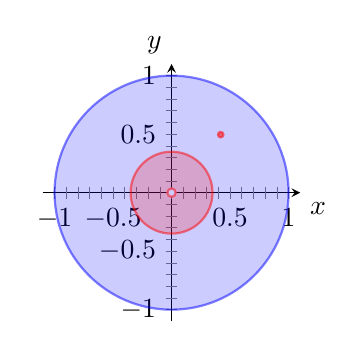
\begin{tikzpicture}
\begin{axis}[%
    width= \linewidth*2/5,
    height= \linewidth*2/5,
    enlargelimits=0,
  axis x line=center,
  axis y line=center,
  xtick={-1,-0.5,...,1},
  ytick={-1,-0.5,...,1},
  xlabel={$x$},
  ylabel={$y$},
  extra x ticks={-0.9,-0.8,...,0.9},
  extra y ticks={-0.9,-0.8,...,0.9},
  extra x tick label={\empty},
  extra y tick label={\empty},
  xlabel style={below right},
  ylabel style={above left},
  xmin=-1.1,
  xmax=1.1,
  ymin=-1.1,
  ymax=1.1]
  \definecolor{auxblue}{rgb}{0.8,0.8,1}
  \draw [fill opacity=0.2, draw opacity=0.5, thick, fill=blue, draw=blue] (0,0) circle (1);
  \draw [fill opacity=0.2, draw opacity=0.5, thick, fill=red, draw=red] (0,0) circle (0.35);
  \draw [fill opacity=0.5, draw opacity=0.5, thick, fill=red, draw=red] (0.42,0.49608467019) circle (1pt);
  \draw [thick, draw opacity=0.5, fill=auxblue, draw=red] (0,0) circle (1.5pt);
  
\end{axis}
\end{tikzpicture}
\caption{$B_1 \left( 0,0 \right)$ y $B_1 \left( \frac{42}{100},\sqrt{\frac{2461}{10}} \right)$}
\end{figure}

\end{eje}

\begin{eje}
    Tenemos que comprobar que
    \begin{enumerate}[i)]
        \item $d(a,b) \geq 0 \; \forall a,b \in A^n$ y que $d(a,b) = 0 \iff a = b$, lo cual es trivial por la definición de $d$.
        \item $d(a,b) = d(b,a) \; \forall a,b \in A^n$. Trivial por la definición.
        \item $d(a, b) \leq d(a,c) + d(c, b)$. Sea $i \in R = \setb{j \vert a_j \neq b_j}$, entonces, se cumple al menos una de las dos siguientes afirmaciones
            \[
                \begin{cases}
                    i \in P = \setb{j \vert a_j \neq c_j} \\
                    i \in Q = \setb{j \vert c_j \neq b_j}
                \end{cases}
            \]
            Por lo tanto, $R \subseteq P \cup Q \implies d(a,b) = \abs{R} \leq \abs{P \cup Q} \leq \abs{P} + \abs{Q} = d(a,c) + d(a,b)$.
    \end{enumerate}
\end{eje}

\begin{eje}
    Tenemos que comprobar que
    \begin{enumerate}[i)]
        \item $d(a,b) \geq 0 \;  \forall a,b \in \mathcal{S}(A)$, y que $d(a,b) = 0 \iff a = b$, lo cual es trivial por la definición.
        \item $d(a,b) = d(b,a) \; \forall a,b \in \mathcal{S}(A)$, tambi\'en trivial por la definición.
        \item $d(a,b) \leq d(a,c) + d(c,b)$. Podemos suponer sin p\'erdida de generalidad que $d(a,c) \geq d(b,c)$. Sea $s$ tal que $e^{-s} = d(a,c)$ y sea
            $S$ tal que $e^{-S} = d(b,c)$, entonces, si $S = s$, entonces, $d(b, c) = d(a,c) \implies d(a, b) \leq d(a,c)$. Si $S > s$, entonces, 
            $d(a, b) \leq d(a,c)$.
    \end{enumerate}
\end{eje}

\begin{eje}
    \begin{enumerate}[(a)]
        \item[]
        \item Sí que define una m\'etrica, ya que
            \begin{enumerate}[i)]
                \item $d(x,y) \geq 0$ y $d(x,y) = 0 \iff x = y$ son triviales.
                \item $d(x,y) = d(y,x)$ es obvio.
                \item $d(x,y) = \abs{e^x - e^y} = \abs{e^x - e^z + e^z - e^y} \leq \abs{e^x - e^z} + \abs{e^z - e^y} = d(x,z) + d(y,z).$
            \end{enumerate}
        \item No es una m\'etrica. Los puntos $x = \frac{\pi}{2}$ y $y = \frac{3\pi}{2}$ son distintos, pero $d(x, y) = 0$.
        \item Sí que es una m\'etrica:
            \begin{enumerate}[i)]
                \item $d(x, y) \geq 0$ es trivial y $d(x,y) = 0 \iff \cos(x) = \cos(y) \iff x = y$.
                \item $d(x, y) = d(y,x)$ es obvio.
                \item Finalmente,
                    \begin{align*}
                        d(x, y) &= \abs{\cos(x) - \cos(y)} \\
                        &= \abs{\cos(x) - \cos(z) + \cos(z) - \cos(y)} \\
                        &\leq \abs{\cos(x) - \cos(z)} + \abs{\cos(z) - \cos(y)} = d(x,z) + d(z,y).
                    \end{align*}
            \end{enumerate}
        \item Sí define una m\'etrica:
            \begin{enumerate}[i)]
                \item $d(x, y) \geq 0$ es trivial y $d(x, y) = 0 \iff \arctan(x) = \arctan(y) \iff x = y$.
                \item $d(x, y) = d(y, x)$ es obvio.
                \item Finalmente,
                    \begin{align*}
                        d(x, y) &= \abs{\arctan(x) - \arctan(y)} \\
                        &= \abs{\arctan(x) - \arctan(z) + \arctan(z) - \arctan(y)} \\
                        &\leq \abs{\arctan(x) - \arctan(z)} + \abs{\arctan(z) - \arctan(y)} \\
                        &= d(x, z) + d(y,z).
                    \end{align*}
            \end{enumerate}
    \end{enumerate}

    En general, basta con que $f$ sea inyectiva para que $d_f(x,y) = \abs{f(x) - f(y)}$ sea una distancia. Vemos que si $f$ es inyectiva
    \begin{enumerate}[i)]
        \item $d(x,y) \geq 0$ por el valor absoluto. $d(x, y) = 0 \iff f(x) - f(y) = 0 \iff f(x) = f(y) \stackrel{f \text{ inyectiva}}{\iff} x = y$.
        \item $d(x,y) = \abs{f(x) - f(y)} = \abs{f(y) - f(x)} = d(y,x)$.
        \item $d(x,y) = \abs{f(x) - f(y)} = \abs{f(x) - f(z) + f(z) - f(y)} \leq \abs{f(x) - f(z)} + \abs{f(z) - f(y)}$ $ = d(x, z) + d(z, y)$.
    \end{enumerate}
\end{eje}

\begin{eje}
    \begin{enumerate}[(a)]
        \item[]
        \item Sí que es una m\'etrica, de hecho es la m\'etrica habitual en $\real^n$.
            \begin{figure}[H]
\centering
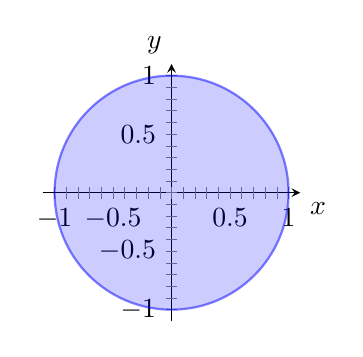
\begin{tikzpicture}
\begin{axis}[%
    width= \linewidth*2/5,
    height= \linewidth*2/5,
    enlargelimits=0,
  axis x line=center,
  axis y line=center,
  xtick={-1,-0.5,...,1},
  ytick={-1,-0.5,...,1},
  xlabel={$x$},
  ylabel={$y$},
  extra x ticks={-0.9,-0.8,...,0.9},
  extra y ticks={-0.9,-0.8,...,0.9},
  extra x tick label={\empty},
  extra y tick label={\empty},
  xlabel style={below right},
  ylabel style={above left},
  xmin=-1.1,
  xmax=1.1,
  ymin=-1.1,
  ymax=1.1]

  \draw [fill opacity=0.2, draw opacity=0.5, thick, fill=blue, draw=blue] (0,0) circle (1);
\end{axis}
\end{tikzpicture}
\caption{$B_1 \left( 0,0 \right)$}
\end{figure}

        \item Sí que es una distancia
            \begin{figure}[H]
\centering
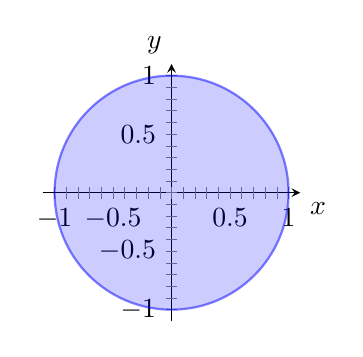
\begin{tikzpicture}
\begin{axis}[%
    width= \linewidth*2/5,
    height= \linewidth*2/5,
    enlargelimits=0,
  axis x line=center,
  axis y line=center,
  xtick={-1,-0.5,...,1},
  ytick={-1,-0.5,...,1},
  xlabel={$x$},
  ylabel={$y$},
  extra x ticks={-0.9,-0.8,...,0.9},
  extra y ticks={-0.9,-0.8,...,0.9},
  extra x tick label={\empty},
  extra y tick label={\empty},
  xlabel style={below right},
  ylabel style={above left},
  xmin=-1.1,
  xmax=1.1,
  ymin=-1.1,
  ymax=1.1]

  \draw [fill opacity=0.2, draw opacity=0.5, thick, fill=blue, draw=blue] (0,0) circle (1);
\end{axis}
\end{tikzpicture}
\caption{$B_1 \left( 0,0 \right)$}
\end{figure}

        \item Sí que es una m\'etrica
            \begin{figure}[H]
\centering
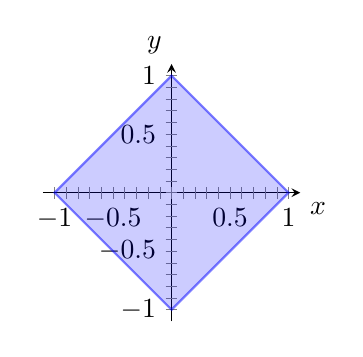
\begin{tikzpicture}
\begin{axis}[%
    width= \linewidth*2/5,
    height= \linewidth*2/5,
    enlargelimits=0,
  axis x line=center,
  axis y line=center,
  xtick={-1,-0.5,...,1},
  ytick={-1,-0.5,...,1},
  xlabel={$x$},
  ylabel={$y$},
  extra x ticks={-0.9,-0.8,...,0.9},
  extra y ticks={-0.9,-0.8,...,0.9},
  extra x tick label={\empty},
  extra y tick label={\empty},
  xlabel style={below right},
  ylabel style={above left},
  xmin=-1.1,
  xmax=1.1,
  ymin=-1.1,
  ymax=1.1]

  \draw [fill opacity=0.2, draw opacity=0.5, thick, fill=blue, draw=blue] (0,-1) -- (-1,0) -- (0,1) -- (1,0) -- cycle;
\end{axis}
\end{tikzpicture}
\caption{$B_1 \left( 0,0 \right)$}
\end{figure}

        \item No es una m\'etrica, por ejemplo, $d\left( (1,0), (1,1) \right) = 0$, pero $(1,0) \neq (1,1)$.
        \item Sí que es una m\'etrica
            \begin{figure}[H]
\centering
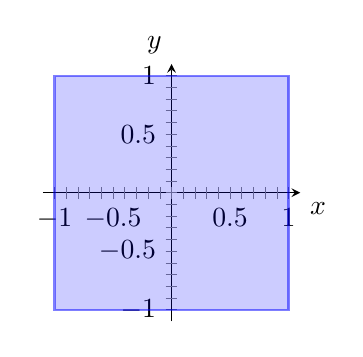
\begin{tikzpicture}
\begin{axis}[%
    width= \linewidth*2/5,
    height= \linewidth*2/5,
    enlargelimits=0,
  axis x line=center,
  axis y line=center,
  xtick={-1,-0.5,...,1},
  ytick={-1,-0.5,...,1},
  xlabel={$x$},
  ylabel={$y$},
  extra x ticks={-0.9,-0.8,...,0.9},
  extra y ticks={-0.9,-0.8,...,0.9},
  extra x tick label={\empty},
  extra y tick label={\empty},
  xlabel style={below right},
  ylabel style={above left},
  xmin=-1.1,
  xmax=1.1,
  ymin=-1.1,
  ymax=1.1]

  \draw [fill opacity=0.2, draw opacity=0.5, thick, fill=blue, draw=blue] (-1,-1) -- (-1,1) -- (1,1) -- (1,-1) -- cycle;
\end{axis}
\end{tikzpicture}
\caption{$B_1 \left( 0,0 \right)$}
\end{figure}

        \item No es una m\'etrica, por ejemplo, $d\left( (1,0), (1,1) \right) = 0$, pero $(1,0) \neq (1,1)$.
        \item En general no  es una m\'etrica, si tomamos la distancia euclidiana, $d_{\text{eq}} \left( (1, 0) , (0.5, 0) \right) = 0.5 \implies
            d\left( (1,0), (0.5, 0) \right) = \lfloor0.5 \rfloor = 0$.
        \item En general no es una m\'etrica, por ejemplo si $A$ tiene un vep $v$ de vap $\lambda < 0$, entonces $d(v, 0) = \sqrt{(v - 0) A (v-0)^t}$ no existe,
            ya que el contenido de dentro de la raiz es negativo.
        \item Vemos que cumple que
            \begin{enumerate}[i)]
                \item $d(x, y) \geq 0$, sí, ya que $A$ es definida positiva y por lo tanto, $(x-y)A(x-y)^t \geq 0 \implies \sqrt{(x-y)A(x-y)^t} \geq 0$.
                \item $d(x, y) = 0 \iff \sqrt{(x-y)A(x-y)^t} = 0 \iff (x-y)A(x-y)^t = 0 \stackrel{A \text{ def. pos.}}{\iff} x = y$.
                \item $d(x, y) = \sqrt{(x-y)A(x-y)^t} = \sqrt{(-1)(y-x)A(-1)(y-x)^t} =$ \\ $\sqrt{(y-x)A(y-x)^t} = d(y, x)$
                \item Se tiene que
                    \begin{align*}
                        d^2(x,y) &= (x-y)A(x-y)^t = (x-z+z-y)A(x-z+z-y)^t \\
                        &= (x-z)A(x-z)^t + (x-z)A(z-y)^t + (z-y)A(x-z)^t\, + \\
                        &\qquad\qquad + (z-y)A(z-y)^t \\
                        &\leq (x-z)A(x-z)^t + 2 \abs{(x-z)A(z-y)^t} + (z-y)A(z-y)^t \\
                        &\leq (x-z)A(x-z)^t + 2 \sqrt{(x-z)A(x-z)^t(z-y)A(z-y)^t} \,\,+ \\
                        &\qquad\qquad + (z-y)A(z-y)^t \\
                        &= \left( (x-z)A(x-z)^t + (z-y)A(z-y)^t \right)^2 \\
                        &= \left( d(x,z) + d(z,y) \right)^2.
                    \end{align*}
                    Por lo tanto, $d(x,y) \leq d(x,z) + d(z,y)$.
            \end{enumerate}
            Ponemos un ejemplo, tomando
            \[
                A =
                \begin{pmatrix}
                    1 & 2 \\
                    2 & 5
                \end{pmatrix}
            \]
            \begin{center}
                %% Creator: Matplotlib, PGF backend
%%
%% To include the figure in your LaTeX document, write
%%   \input{<filename>.pgf}
%%
%% Make sure the required packages are loaded in your preamble
%%   \usepackage{pgf}
%%
%% Figures using additional raster images can only be included by \input if
%% they are in the same directory as the main LaTeX file. For loading figures
%% from other directories you can use the `import` package
%%   \usepackage{import}
%% and then include the figures with
%%   \import{<path to file>}{<filename>.pgf}
%%
%% Matplotlib used the following preamble
%%   \usepackage{fontspec}
%%   \setmainfont{DejaVu Serif}
%%   \setsansfont{DejaVu Sans}
%%   \setmonofont{DejaVu Sans Mono}
%%
\begingroup%
\makeatletter%
\begin{pgfpicture}%
\pgfpathrectangle{\pgfpointorigin}{\pgfqpoint{4.900000in}{1.830305in}}%
\pgfusepath{use as bounding box, clip}%
\begin{pgfscope}%
\pgfsetbuttcap%
\pgfsetmiterjoin%
\definecolor{currentfill}{rgb}{1.000000,1.000000,1.000000}%
\pgfsetfillcolor{currentfill}%
\pgfsetlinewidth{0.000000pt}%
\definecolor{currentstroke}{rgb}{1.000000,1.000000,1.000000}%
\pgfsetstrokecolor{currentstroke}%
\pgfsetdash{}{0pt}%
\pgfpathmoveto{\pgfqpoint{0.000000in}{-0.000000in}}%
\pgfpathlineto{\pgfqpoint{4.900000in}{-0.000000in}}%
\pgfpathlineto{\pgfqpoint{4.900000in}{1.830305in}}%
\pgfpathlineto{\pgfqpoint{0.000000in}{1.830305in}}%
\pgfpathclose%
\pgfusepath{fill}%
\end{pgfscope}%
\begin{pgfscope}%
\pgfsetbuttcap%
\pgfsetmiterjoin%
\definecolor{currentfill}{rgb}{1.000000,1.000000,1.000000}%
\pgfsetfillcolor{currentfill}%
\pgfsetlinewidth{0.000000pt}%
\definecolor{currentstroke}{rgb}{0.000000,0.000000,0.000000}%
\pgfsetstrokecolor{currentstroke}%
\pgfsetstrokeopacity{0.000000}%
\pgfsetdash{}{0pt}%
\pgfpathmoveto{\pgfqpoint{0.135000in}{0.151972in}}%
\pgfpathlineto{\pgfqpoint{4.765000in}{0.151972in}}%
\pgfpathlineto{\pgfqpoint{4.765000in}{1.695305in}}%
\pgfpathlineto{\pgfqpoint{0.135000in}{1.695305in}}%
\pgfpathclose%
\pgfusepath{fill}%
\end{pgfscope}%
\begin{pgfscope}%
\pgfpathrectangle{\pgfqpoint{0.135000in}{0.151972in}}{\pgfqpoint{4.630000in}{1.543333in}} %
\pgfusepath{clip}%
\pgfsetbuttcap%
\pgfsetroundjoin%
\definecolor{currentfill}{rgb}{0.000000,0.000000,1.000000}%
\pgfsetfillcolor{currentfill}%
\pgfsetfillopacity{0.300000}%
\pgfsetlinewidth{0.000000pt}%
\definecolor{currentstroke}{rgb}{0.000000,0.000000,0.000000}%
\pgfsetstrokecolor{currentstroke}%
\pgfsetdash{}{0pt}%
\pgfpathmoveto{\pgfqpoint{3.809480in}{0.189659in}}%
\pgfpathlineto{\pgfqpoint{3.839359in}{0.186570in}}%
\pgfpathlineto{\pgfqpoint{3.869237in}{0.184112in}}%
\pgfpathlineto{\pgfqpoint{3.899116in}{0.182418in}}%
\pgfpathlineto{\pgfqpoint{3.928995in}{0.181668in}}%
\pgfpathlineto{\pgfqpoint{3.958873in}{0.182113in}}%
\pgfpathlineto{\pgfqpoint{3.988752in}{0.184110in}}%
\pgfpathlineto{\pgfqpoint{4.018631in}{0.188182in}}%
\pgfpathlineto{\pgfqpoint{4.034320in}{0.191611in}}%
\pgfpathlineto{\pgfqpoint{4.048509in}{0.195478in}}%
\pgfpathlineto{\pgfqpoint{4.064288in}{0.201570in}}%
\pgfpathlineto{\pgfqpoint{4.078388in}{0.208846in}}%
\pgfpathlineto{\pgfqpoint{4.082426in}{0.211530in}}%
\pgfpathlineto{\pgfqpoint{4.093739in}{0.221489in}}%
\pgfpathlineto{\pgfqpoint{4.101361in}{0.231449in}}%
\pgfpathlineto{\pgfqpoint{4.106103in}{0.241409in}}%
\pgfpathlineto{\pgfqpoint{4.108267in}{0.250123in}}%
\pgfpathlineto{\pgfqpoint{4.108533in}{0.251368in}}%
\pgfpathlineto{\pgfqpoint{4.109092in}{0.261328in}}%
\pgfpathlineto{\pgfqpoint{4.108267in}{0.270872in}}%
\pgfpathlineto{\pgfqpoint{4.108230in}{0.271287in}}%
\pgfpathlineto{\pgfqpoint{4.106039in}{0.281247in}}%
\pgfpathlineto{\pgfqpoint{4.102777in}{0.291206in}}%
\pgfpathlineto{\pgfqpoint{4.098596in}{0.301166in}}%
\pgfpathlineto{\pgfqpoint{4.093620in}{0.311126in}}%
\pgfpathlineto{\pgfqpoint{4.087943in}{0.321085in}}%
\pgfpathlineto{\pgfqpoint{4.081644in}{0.331045in}}%
\pgfpathlineto{\pgfqpoint{4.078388in}{0.335681in}}%
\pgfpathlineto{\pgfqpoint{4.074638in}{0.341004in}}%
\pgfpathlineto{\pgfqpoint{4.067009in}{0.350964in}}%
\pgfpathlineto{\pgfqpoint{4.058939in}{0.360923in}}%
\pgfpathlineto{\pgfqpoint{4.050462in}{0.370883in}}%
\pgfpathlineto{\pgfqpoint{4.048509in}{0.373028in}}%
\pgfpathlineto{\pgfqpoint{4.041388in}{0.380842in}}%
\pgfpathlineto{\pgfqpoint{4.031926in}{0.390802in}}%
\pgfpathlineto{\pgfqpoint{4.022156in}{0.400762in}}%
\pgfpathlineto{\pgfqpoint{4.018631in}{0.404191in}}%
\pgfpathlineto{\pgfqpoint{4.011918in}{0.410721in}}%
\pgfpathlineto{\pgfqpoint{4.001332in}{0.420681in}}%
\pgfpathlineto{\pgfqpoint{3.990502in}{0.430640in}}%
\pgfpathlineto{\pgfqpoint{3.988752in}{0.432184in}}%
\pgfpathlineto{\pgfqpoint{3.979225in}{0.440600in}}%
\pgfpathlineto{\pgfqpoint{3.967706in}{0.450559in}}%
\pgfpathlineto{\pgfqpoint{3.958873in}{0.458022in}}%
\pgfpathlineto{\pgfqpoint{3.955923in}{0.460519in}}%
\pgfpathlineto{\pgfqpoint{3.943779in}{0.470478in}}%
\pgfpathlineto{\pgfqpoint{3.931460in}{0.480438in}}%
\pgfpathlineto{\pgfqpoint{3.928995in}{0.482373in}}%
\pgfpathlineto{\pgfqpoint{3.918792in}{0.490398in}}%
\pgfpathlineto{\pgfqpoint{3.905929in}{0.500357in}}%
\pgfpathlineto{\pgfqpoint{3.899116in}{0.505524in}}%
\pgfpathlineto{\pgfqpoint{3.892812in}{0.510317in}}%
\pgfpathlineto{\pgfqpoint{3.879448in}{0.520276in}}%
\pgfpathlineto{\pgfqpoint{3.869237in}{0.527775in}}%
\pgfpathlineto{\pgfqpoint{3.865895in}{0.530236in}}%
\pgfpathlineto{\pgfqpoint{3.852070in}{0.540195in}}%
\pgfpathlineto{\pgfqpoint{3.839359in}{0.549252in}}%
\pgfpathlineto{\pgfqpoint{3.838095in}{0.550155in}}%
\pgfpathlineto{\pgfqpoint{3.823841in}{0.560115in}}%
\pgfpathlineto{\pgfqpoint{3.809480in}{0.570061in}}%
\pgfpathlineto{\pgfqpoint{3.809461in}{0.570074in}}%
\pgfpathlineto{\pgfqpoint{3.794806in}{0.580034in}}%
\pgfpathlineto{\pgfqpoint{3.780030in}{0.589993in}}%
\pgfpathlineto{\pgfqpoint{3.779601in}{0.590276in}}%
\pgfpathlineto{\pgfqpoint{3.765002in}{0.599953in}}%
\pgfpathlineto{\pgfqpoint{3.749851in}{0.609912in}}%
\pgfpathlineto{\pgfqpoint{3.749723in}{0.609995in}}%
\pgfpathlineto{\pgfqpoint{3.734463in}{0.619872in}}%
\pgfpathlineto{\pgfqpoint{3.719844in}{0.629256in}}%
\pgfpathlineto{\pgfqpoint{3.718950in}{0.629831in}}%
\pgfpathlineto{\pgfqpoint{3.703219in}{0.639791in}}%
\pgfpathlineto{\pgfqpoint{3.689965in}{0.648108in}}%
\pgfpathlineto{\pgfqpoint{3.687356in}{0.649751in}}%
\pgfpathlineto{\pgfqpoint{3.671298in}{0.659710in}}%
\pgfpathlineto{\pgfqpoint{3.660086in}{0.666596in}}%
\pgfpathlineto{\pgfqpoint{3.655096in}{0.669670in}}%
\pgfpathlineto{\pgfqpoint{3.638722in}{0.679629in}}%
\pgfpathlineto{\pgfqpoint{3.630208in}{0.684752in}}%
\pgfpathlineto{\pgfqpoint{3.622193in}{0.689589in}}%
\pgfpathlineto{\pgfqpoint{3.605511in}{0.699548in}}%
\pgfpathlineto{\pgfqpoint{3.600329in}{0.702606in}}%
\pgfpathlineto{\pgfqpoint{3.588666in}{0.709508in}}%
\pgfpathlineto{\pgfqpoint{3.571684in}{0.719467in}}%
\pgfpathlineto{\pgfqpoint{3.570450in}{0.720182in}}%
\pgfpathlineto{\pgfqpoint{3.554532in}{0.729427in}}%
\pgfpathlineto{\pgfqpoint{3.540572in}{0.737466in}}%
\pgfpathlineto{\pgfqpoint{3.537246in}{0.739387in}}%
\pgfpathlineto{\pgfqpoint{3.519804in}{0.749346in}}%
\pgfpathlineto{\pgfqpoint{3.510693in}{0.754501in}}%
\pgfpathlineto{\pgfqpoint{3.502220in}{0.759306in}}%
\pgfpathlineto{\pgfqpoint{3.484494in}{0.769265in}}%
\pgfpathlineto{\pgfqpoint{3.480814in}{0.771312in}}%
\pgfpathlineto{\pgfqpoint{3.466619in}{0.779225in}}%
\pgfpathlineto{\pgfqpoint{3.450936in}{0.787896in}}%
\pgfpathlineto{\pgfqpoint{3.448610in}{0.789184in}}%
\pgfpathlineto{\pgfqpoint{3.430454in}{0.799144in}}%
\pgfpathlineto{\pgfqpoint{3.421057in}{0.804255in}}%
\pgfpathlineto{\pgfqpoint{3.412161in}{0.809103in}}%
\pgfpathlineto{\pgfqpoint{3.393731in}{0.819063in}}%
\pgfpathlineto{\pgfqpoint{3.391178in}{0.820430in}}%
\pgfpathlineto{\pgfqpoint{3.375159in}{0.829023in}}%
\pgfpathlineto{\pgfqpoint{3.361300in}{0.836399in}}%
\pgfpathlineto{\pgfqpoint{3.356453in}{0.838982in}}%
\pgfpathlineto{\pgfqpoint{3.337610in}{0.848942in}}%
\pgfpathlineto{\pgfqpoint{3.331421in}{0.852187in}}%
\pgfpathlineto{\pgfqpoint{3.318631in}{0.858901in}}%
\pgfpathlineto{\pgfqpoint{3.301542in}{0.867805in}}%
\pgfpathlineto{\pgfqpoint{3.299517in}{0.868861in}}%
\pgfpathlineto{\pgfqpoint{3.280268in}{0.878820in}}%
\pgfpathlineto{\pgfqpoint{3.271664in}{0.883240in}}%
\pgfpathlineto{\pgfqpoint{3.260885in}{0.888780in}}%
\pgfpathlineto{\pgfqpoint{3.241785in}{0.898526in}}%
\pgfpathlineto{\pgfqpoint{3.241367in}{0.898740in}}%
\pgfpathlineto{\pgfqpoint{3.221715in}{0.908699in}}%
\pgfpathlineto{\pgfqpoint{3.211906in}{0.913636in}}%
\pgfpathlineto{\pgfqpoint{3.201930in}{0.918659in}}%
\pgfpathlineto{\pgfqpoint{3.182028in}{0.928610in}}%
\pgfpathlineto{\pgfqpoint{3.182011in}{0.928618in}}%
\pgfpathlineto{\pgfqpoint{3.161958in}{0.938578in}}%
\pgfpathlineto{\pgfqpoint{3.152149in}{0.943418in}}%
\pgfpathlineto{\pgfqpoint{3.141771in}{0.948537in}}%
\pgfpathlineto{\pgfqpoint{3.122270in}{0.958096in}}%
\pgfpathlineto{\pgfqpoint{3.121451in}{0.958497in}}%
\pgfpathlineto{\pgfqpoint{3.100996in}{0.968456in}}%
\pgfpathlineto{\pgfqpoint{3.092392in}{0.972621in}}%
\pgfpathlineto{\pgfqpoint{3.080406in}{0.978416in}}%
\pgfpathlineto{\pgfqpoint{3.062513in}{0.987017in}}%
\pgfpathlineto{\pgfqpoint{3.059683in}{0.988376in}}%
\pgfpathlineto{\pgfqpoint{3.038823in}{0.998335in}}%
\pgfpathlineto{\pgfqpoint{3.032634in}{1.001274in}}%
\pgfpathlineto{\pgfqpoint{3.017827in}{1.008295in}}%
\pgfpathlineto{\pgfqpoint{3.002756in}{1.015402in}}%
\pgfpathlineto{\pgfqpoint{2.996697in}{1.018254in}}%
\pgfpathlineto{\pgfqpoint{2.975429in}{1.028214in}}%
\pgfpathlineto{\pgfqpoint{2.972877in}{1.029403in}}%
\pgfpathlineto{\pgfqpoint{2.954021in}{1.038173in}}%
\pgfpathlineto{\pgfqpoint{2.942998in}{1.043275in}}%
\pgfpathlineto{\pgfqpoint{2.932475in}{1.048133in}}%
\pgfpathlineto{\pgfqpoint{2.913120in}{1.057027in}}%
\pgfpathlineto{\pgfqpoint{2.910794in}{1.058092in}}%
\pgfpathlineto{\pgfqpoint{2.888967in}{1.068052in}}%
\pgfpathlineto{\pgfqpoint{2.883241in}{1.070654in}}%
\pgfpathlineto{\pgfqpoint{2.866998in}{1.078012in}}%
\pgfpathlineto{\pgfqpoint{2.853362in}{1.084162in}}%
\pgfpathlineto{\pgfqpoint{2.844889in}{1.087971in}}%
\pgfpathlineto{\pgfqpoint{2.823483in}{1.097555in}}%
\pgfpathlineto{\pgfqpoint{2.822641in}{1.097931in}}%
\pgfpathlineto{\pgfqpoint{2.800236in}{1.107890in}}%
\pgfpathlineto{\pgfqpoint{2.793605in}{1.110828in}}%
\pgfpathlineto{\pgfqpoint{2.777686in}{1.117850in}}%
\pgfpathlineto{\pgfqpoint{2.763726in}{1.123987in}}%
\pgfpathlineto{\pgfqpoint{2.754992in}{1.127809in}}%
\pgfpathlineto{\pgfqpoint{2.733847in}{1.137034in}}%
\pgfpathlineto{\pgfqpoint{2.732154in}{1.137769in}}%
\pgfpathlineto{\pgfqpoint{2.709151in}{1.147729in}}%
\pgfpathlineto{\pgfqpoint{2.703969in}{1.149966in}}%
\pgfpathlineto{\pgfqpoint{2.685992in}{1.157688in}}%
\pgfpathlineto{\pgfqpoint{2.674090in}{1.162788in}}%
\pgfpathlineto{\pgfqpoint{2.662682in}{1.167648in}}%
\pgfpathlineto{\pgfqpoint{2.644211in}{1.175499in}}%
\pgfpathlineto{\pgfqpoint{2.639221in}{1.177607in}}%
\pgfpathlineto{\pgfqpoint{2.615600in}{1.187567in}}%
\pgfpathlineto{\pgfqpoint{2.614333in}{1.188100in}}%
\pgfpathlineto{\pgfqpoint{2.591795in}{1.197526in}}%
\pgfpathlineto{\pgfqpoint{2.584454in}{1.200592in}}%
\pgfpathlineto{\pgfqpoint{2.567829in}{1.207486in}}%
\pgfpathlineto{\pgfqpoint{2.554575in}{1.212975in}}%
\pgfpathlineto{\pgfqpoint{2.543701in}{1.217445in}}%
\pgfpathlineto{\pgfqpoint{2.524697in}{1.225250in}}%
\pgfpathlineto{\pgfqpoint{2.519407in}{1.227405in}}%
\pgfpathlineto{\pgfqpoint{2.494947in}{1.237365in}}%
\pgfpathlineto{\pgfqpoint{2.494818in}{1.237417in}}%
\pgfpathlineto{\pgfqpoint{2.470272in}{1.247324in}}%
\pgfpathlineto{\pgfqpoint{2.464939in}{1.249476in}}%
\pgfpathlineto{\pgfqpoint{2.445420in}{1.257284in}}%
\pgfpathlineto{\pgfqpoint{2.435061in}{1.261427in}}%
\pgfpathlineto{\pgfqpoint{2.420387in}{1.267243in}}%
\pgfpathlineto{\pgfqpoint{2.405182in}{1.273271in}}%
\pgfpathlineto{\pgfqpoint{2.395168in}{1.277203in}}%
\pgfpathlineto{\pgfqpoint{2.375303in}{1.285007in}}%
\pgfpathlineto{\pgfqpoint{2.369761in}{1.287162in}}%
\pgfpathlineto{\pgfqpoint{2.345425in}{1.296636in}}%
\pgfpathlineto{\pgfqpoint{2.344161in}{1.297122in}}%
\pgfpathlineto{\pgfqpoint{2.318328in}{1.307081in}}%
\pgfpathlineto{\pgfqpoint{2.315546in}{1.308155in}}%
\pgfpathlineto{\pgfqpoint{2.292271in}{1.317041in}}%
\pgfpathlineto{\pgfqpoint{2.285667in}{1.319566in}}%
\pgfpathlineto{\pgfqpoint{2.266000in}{1.327001in}}%
\pgfpathlineto{\pgfqpoint{2.255789in}{1.330868in}}%
\pgfpathlineto{\pgfqpoint{2.239507in}{1.336960in}}%
\pgfpathlineto{\pgfqpoint{2.225910in}{1.342060in}}%
\pgfpathlineto{\pgfqpoint{2.212786in}{1.346920in}}%
\pgfpathlineto{\pgfqpoint{2.196031in}{1.353141in}}%
\pgfpathlineto{\pgfqpoint{2.185829in}{1.356879in}}%
\pgfpathlineto{\pgfqpoint{2.166153in}{1.364111in}}%
\pgfpathlineto{\pgfqpoint{2.158626in}{1.366839in}}%
\pgfpathlineto{\pgfqpoint{2.136274in}{1.374969in}}%
\pgfpathlineto{\pgfqpoint{2.131169in}{1.376798in}}%
\pgfpathlineto{\pgfqpoint{2.106395in}{1.385712in}}%
\pgfpathlineto{\pgfqpoint{2.103445in}{1.386758in}}%
\pgfpathlineto{\pgfqpoint{2.076517in}{1.396342in}}%
\pgfpathlineto{\pgfqpoint{2.075443in}{1.396718in}}%
\pgfpathlineto{\pgfqpoint{2.047139in}{1.406677in}}%
\pgfpathlineto{\pgfqpoint{2.046638in}{1.406854in}}%
\pgfpathlineto{\pgfqpoint{2.018509in}{1.416637in}}%
\pgfpathlineto{\pgfqpoint{2.016759in}{1.417248in}}%
\pgfpathlineto{\pgfqpoint{1.989562in}{1.426596in}}%
\pgfpathlineto{\pgfqpoint{1.986880in}{1.427523in}}%
\pgfpathlineto{\pgfqpoint{1.960281in}{1.436556in}}%
\pgfpathlineto{\pgfqpoint{1.957002in}{1.437676in}}%
\pgfpathlineto{\pgfqpoint{1.930649in}{1.446515in}}%
\pgfpathlineto{\pgfqpoint{1.927123in}{1.447705in}}%
\pgfpathlineto{\pgfqpoint{1.900646in}{1.456475in}}%
\pgfpathlineto{\pgfqpoint{1.897244in}{1.457609in}}%
\pgfpathlineto{\pgfqpoint{1.870251in}{1.466434in}}%
\pgfpathlineto{\pgfqpoint{1.867366in}{1.467384in}}%
\pgfpathlineto{\pgfqpoint{1.839440in}{1.476394in}}%
\pgfpathlineto{\pgfqpoint{1.837487in}{1.477029in}}%
\pgfpathlineto{\pgfqpoint{1.808189in}{1.486354in}}%
\pgfpathlineto{\pgfqpoint{1.807608in}{1.486540in}}%
\pgfpathlineto{\pgfqpoint{1.777730in}{1.495912in}}%
\pgfpathlineto{\pgfqpoint{1.776420in}{1.496313in}}%
\pgfpathlineto{\pgfqpoint{1.747851in}{1.505142in}}%
\pgfpathlineto{\pgfqpoint{1.744102in}{1.506273in}}%
\pgfpathlineto{\pgfqpoint{1.717972in}{1.514227in}}%
\pgfpathlineto{\pgfqpoint{1.711216in}{1.516232in}}%
\pgfpathlineto{\pgfqpoint{1.688094in}{1.523163in}}%
\pgfpathlineto{\pgfqpoint{1.677721in}{1.526192in}}%
\pgfpathlineto{\pgfqpoint{1.658215in}{1.531945in}}%
\pgfpathlineto{\pgfqpoint{1.643568in}{1.536151in}}%
\pgfpathlineto{\pgfqpoint{1.628336in}{1.540571in}}%
\pgfpathlineto{\pgfqpoint{1.608704in}{1.546111in}}%
\pgfpathlineto{\pgfqpoint{1.598458in}{1.549034in}}%
\pgfpathlineto{\pgfqpoint{1.573070in}{1.556070in}}%
\pgfpathlineto{\pgfqpoint{1.568579in}{1.557329in}}%
\pgfpathlineto{\pgfqpoint{1.538700in}{1.565446in}}%
\pgfpathlineto{\pgfqpoint{1.536473in}{1.566030in}}%
\pgfpathlineto{\pgfqpoint{1.508822in}{1.573368in}}%
\pgfpathlineto{\pgfqpoint{1.498606in}{1.575990in}}%
\pgfpathlineto{\pgfqpoint{1.478943in}{1.581101in}}%
\pgfpathlineto{\pgfqpoint{1.459636in}{1.585949in}}%
\pgfpathlineto{\pgfqpoint{1.449064in}{1.588639in}}%
\pgfpathlineto{\pgfqpoint{1.419452in}{1.595909in}}%
\pgfpathlineto{\pgfqpoint{1.419186in}{1.595975in}}%
\pgfpathlineto{\pgfqpoint{1.389307in}{1.603059in}}%
\pgfpathlineto{\pgfqpoint{1.376957in}{1.605868in}}%
\pgfpathlineto{\pgfqpoint{1.359428in}{1.609917in}}%
\pgfpathlineto{\pgfqpoint{1.332728in}{1.615828in}}%
\pgfpathlineto{\pgfqpoint{1.329550in}{1.616542in}}%
\pgfpathlineto{\pgfqpoint{1.299671in}{1.622870in}}%
\pgfpathlineto{\pgfqpoint{1.285143in}{1.625787in}}%
\pgfpathlineto{\pgfqpoint{1.269792in}{1.628922in}}%
\pgfpathlineto{\pgfqpoint{1.239914in}{1.634678in}}%
\pgfpathlineto{\pgfqpoint{1.233902in}{1.635747in}}%
\pgfpathlineto{\pgfqpoint{1.210035in}{1.640067in}}%
\pgfpathlineto{\pgfqpoint{1.180156in}{1.645131in}}%
\pgfpathlineto{\pgfqpoint{1.176358in}{1.645706in}}%
\pgfpathlineto{\pgfqpoint{1.150277in}{1.649739in}}%
\pgfpathlineto{\pgfqpoint{1.120399in}{1.653938in}}%
\pgfpathlineto{\pgfqpoint{1.106210in}{1.655666in}}%
\pgfpathlineto{\pgfqpoint{1.090520in}{1.657618in}}%
\pgfpathlineto{\pgfqpoint{1.060641in}{1.660707in}}%
\pgfpathlineto{\pgfqpoint{1.030763in}{1.663165in}}%
\pgfpathlineto{\pgfqpoint{1.000884in}{1.664859in}}%
\pgfpathlineto{\pgfqpoint{0.971005in}{1.665609in}}%
\pgfpathlineto{\pgfqpoint{0.941127in}{1.665164in}}%
\pgfpathlineto{\pgfqpoint{0.911248in}{1.663166in}}%
\pgfpathlineto{\pgfqpoint{0.881369in}{1.659095in}}%
\pgfpathlineto{\pgfqpoint{0.865680in}{1.655666in}}%
\pgfpathlineto{\pgfqpoint{0.851491in}{1.651799in}}%
\pgfpathlineto{\pgfqpoint{0.835712in}{1.645706in}}%
\pgfpathlineto{\pgfqpoint{0.821612in}{1.638431in}}%
\pgfpathlineto{\pgfqpoint{0.817574in}{1.635747in}}%
\pgfpathlineto{\pgfqpoint{0.806261in}{1.625787in}}%
\pgfpathlineto{\pgfqpoint{0.798639in}{1.615828in}}%
\pgfpathlineto{\pgfqpoint{0.793897in}{1.605868in}}%
\pgfpathlineto{\pgfqpoint{0.791733in}{1.597154in}}%
\pgfpathlineto{\pgfqpoint{0.791467in}{1.595909in}}%
\pgfpathlineto{\pgfqpoint{0.790908in}{1.585949in}}%
\pgfpathlineto{\pgfqpoint{0.791733in}{1.576404in}}%
\pgfpathlineto{\pgfqpoint{0.791770in}{1.575990in}}%
\pgfpathlineto{\pgfqpoint{0.793961in}{1.566030in}}%
\pgfpathlineto{\pgfqpoint{0.797223in}{1.556070in}}%
\pgfpathlineto{\pgfqpoint{0.801404in}{1.546111in}}%
\pgfpathlineto{\pgfqpoint{0.806380in}{1.536151in}}%
\pgfpathlineto{\pgfqpoint{0.812057in}{1.526192in}}%
\pgfpathlineto{\pgfqpoint{0.818356in}{1.516232in}}%
\pgfpathlineto{\pgfqpoint{0.821612in}{1.511595in}}%
\pgfpathlineto{\pgfqpoint{0.825362in}{1.506273in}}%
\pgfpathlineto{\pgfqpoint{0.832991in}{1.496313in}}%
\pgfpathlineto{\pgfqpoint{0.841061in}{1.486354in}}%
\pgfpathlineto{\pgfqpoint{0.849538in}{1.476394in}}%
\pgfpathlineto{\pgfqpoint{0.851491in}{1.474249in}}%
\pgfpathlineto{\pgfqpoint{0.858612in}{1.466434in}}%
\pgfpathlineto{\pgfqpoint{0.868074in}{1.456475in}}%
\pgfpathlineto{\pgfqpoint{0.877844in}{1.446515in}}%
\pgfpathlineto{\pgfqpoint{0.881369in}{1.443086in}}%
\pgfpathlineto{\pgfqpoint{0.888082in}{1.436556in}}%
\pgfpathlineto{\pgfqpoint{0.898668in}{1.426596in}}%
\pgfpathlineto{\pgfqpoint{0.909498in}{1.416637in}}%
\pgfpathlineto{\pgfqpoint{0.911248in}{1.415092in}}%
\pgfpathlineto{\pgfqpoint{0.920775in}{1.406677in}}%
\pgfpathlineto{\pgfqpoint{0.932294in}{1.396718in}}%
\pgfpathlineto{\pgfqpoint{0.941127in}{1.389255in}}%
\pgfpathlineto{\pgfqpoint{0.944077in}{1.386758in}}%
\pgfpathlineto{\pgfqpoint{0.956221in}{1.376798in}}%
\pgfpathlineto{\pgfqpoint{0.968540in}{1.366839in}}%
\pgfpathlineto{\pgfqpoint{0.971005in}{1.364904in}}%
\pgfpathlineto{\pgfqpoint{0.981208in}{1.356879in}}%
\pgfpathlineto{\pgfqpoint{0.994071in}{1.346920in}}%
\pgfpathlineto{\pgfqpoint{1.000884in}{1.341753in}}%
\pgfpathlineto{\pgfqpoint{1.007188in}{1.336960in}}%
\pgfpathlineto{\pgfqpoint{1.020552in}{1.327001in}}%
\pgfpathlineto{\pgfqpoint{1.030763in}{1.319502in}}%
\pgfpathlineto{\pgfqpoint{1.034105in}{1.317041in}}%
\pgfpathlineto{\pgfqpoint{1.047930in}{1.307081in}}%
\pgfpathlineto{\pgfqpoint{1.060641in}{1.298024in}}%
\pgfpathlineto{\pgfqpoint{1.061905in}{1.297122in}}%
\pgfpathlineto{\pgfqpoint{1.076159in}{1.287162in}}%
\pgfpathlineto{\pgfqpoint{1.090520in}{1.277216in}}%
\pgfpathlineto{\pgfqpoint{1.090539in}{1.277203in}}%
\pgfpathlineto{\pgfqpoint{1.105194in}{1.267243in}}%
\pgfpathlineto{\pgfqpoint{1.119970in}{1.257284in}}%
\pgfpathlineto{\pgfqpoint{1.120399in}{1.257000in}}%
\pgfpathlineto{\pgfqpoint{1.134998in}{1.247324in}}%
\pgfpathlineto{\pgfqpoint{1.150149in}{1.237365in}}%
\pgfpathlineto{\pgfqpoint{1.150277in}{1.237282in}}%
\pgfpathlineto{\pgfqpoint{1.165537in}{1.227405in}}%
\pgfpathlineto{\pgfqpoint{1.180156in}{1.218021in}}%
\pgfpathlineto{\pgfqpoint{1.181050in}{1.217445in}}%
\pgfpathlineto{\pgfqpoint{1.196781in}{1.207486in}}%
\pgfpathlineto{\pgfqpoint{1.210035in}{1.199169in}}%
\pgfpathlineto{\pgfqpoint{1.212644in}{1.197526in}}%
\pgfpathlineto{\pgfqpoint{1.228702in}{1.187567in}}%
\pgfpathlineto{\pgfqpoint{1.239914in}{1.180681in}}%
\pgfpathlineto{\pgfqpoint{1.244904in}{1.177607in}}%
\pgfpathlineto{\pgfqpoint{1.261278in}{1.167648in}}%
\pgfpathlineto{\pgfqpoint{1.269792in}{1.162525in}}%
\pgfpathlineto{\pgfqpoint{1.277807in}{1.157688in}}%
\pgfpathlineto{\pgfqpoint{1.294489in}{1.147729in}}%
\pgfpathlineto{\pgfqpoint{1.299671in}{1.144670in}}%
\pgfpathlineto{\pgfqpoint{1.311334in}{1.137769in}}%
\pgfpathlineto{\pgfqpoint{1.328316in}{1.127809in}}%
\pgfpathlineto{\pgfqpoint{1.329550in}{1.127095in}}%
\pgfpathlineto{\pgfqpoint{1.345468in}{1.117850in}}%
\pgfpathlineto{\pgfqpoint{1.359428in}{1.109810in}}%
\pgfpathlineto{\pgfqpoint{1.362754in}{1.107890in}}%
\pgfpathlineto{\pgfqpoint{1.380196in}{1.097931in}}%
\pgfpathlineto{\pgfqpoint{1.389307in}{1.092776in}}%
\pgfpathlineto{\pgfqpoint{1.397780in}{1.087971in}}%
\pgfpathlineto{\pgfqpoint{1.415506in}{1.078012in}}%
\pgfpathlineto{\pgfqpoint{1.419186in}{1.075965in}}%
\pgfpathlineto{\pgfqpoint{1.433381in}{1.068052in}}%
\pgfpathlineto{\pgfqpoint{1.449064in}{1.059381in}}%
\pgfpathlineto{\pgfqpoint{1.451390in}{1.058092in}}%
\pgfpathlineto{\pgfqpoint{1.469546in}{1.048133in}}%
\pgfpathlineto{\pgfqpoint{1.478943in}{1.043021in}}%
\pgfpathlineto{\pgfqpoint{1.487839in}{1.038173in}}%
\pgfpathlineto{\pgfqpoint{1.506269in}{1.028214in}}%
\pgfpathlineto{\pgfqpoint{1.508822in}{1.026847in}}%
\pgfpathlineto{\pgfqpoint{1.524841in}{1.018254in}}%
\pgfpathlineto{\pgfqpoint{1.538700in}{1.010878in}}%
\pgfpathlineto{\pgfqpoint{1.543547in}{1.008295in}}%
\pgfpathlineto{\pgfqpoint{1.562390in}{0.998335in}}%
\pgfpathlineto{\pgfqpoint{1.568579in}{0.995090in}}%
\pgfpathlineto{\pgfqpoint{1.581369in}{0.988376in}}%
\pgfpathlineto{\pgfqpoint{1.598458in}{0.979472in}}%
\pgfpathlineto{\pgfqpoint{1.600483in}{0.978416in}}%
\pgfpathlineto{\pgfqpoint{1.619732in}{0.968456in}}%
\pgfpathlineto{\pgfqpoint{1.628336in}{0.964037in}}%
\pgfpathlineto{\pgfqpoint{1.639115in}{0.958497in}}%
\pgfpathlineto{\pgfqpoint{1.658215in}{0.948751in}}%
\pgfpathlineto{\pgfqpoint{1.658633in}{0.948537in}}%
\pgfpathlineto{\pgfqpoint{1.678285in}{0.938578in}}%
\pgfpathlineto{\pgfqpoint{1.688094in}{0.933641in}}%
\pgfpathlineto{\pgfqpoint{1.698070in}{0.928618in}}%
\pgfpathlineto{\pgfqpoint{1.717972in}{0.918667in}}%
\pgfpathlineto{\pgfqpoint{1.717989in}{0.918659in}}%
\pgfpathlineto{\pgfqpoint{1.738042in}{0.908699in}}%
\pgfpathlineto{\pgfqpoint{1.747851in}{0.903859in}}%
\pgfpathlineto{\pgfqpoint{1.758229in}{0.898740in}}%
\pgfpathlineto{\pgfqpoint{1.777730in}{0.889181in}}%
\pgfpathlineto{\pgfqpoint{1.778549in}{0.888780in}}%
\pgfpathlineto{\pgfqpoint{1.799004in}{0.878820in}}%
\pgfpathlineto{\pgfqpoint{1.807608in}{0.874656in}}%
\pgfpathlineto{\pgfqpoint{1.819594in}{0.868861in}}%
\pgfpathlineto{\pgfqpoint{1.837487in}{0.860260in}}%
\pgfpathlineto{\pgfqpoint{1.840317in}{0.858901in}}%
\pgfpathlineto{\pgfqpoint{1.861177in}{0.848942in}}%
\pgfpathlineto{\pgfqpoint{1.867366in}{0.846003in}}%
\pgfpathlineto{\pgfqpoint{1.882173in}{0.838982in}}%
\pgfpathlineto{\pgfqpoint{1.897244in}{0.831875in}}%
\pgfpathlineto{\pgfqpoint{1.903303in}{0.829023in}}%
\pgfpathlineto{\pgfqpoint{1.924571in}{0.819063in}}%
\pgfpathlineto{\pgfqpoint{1.927123in}{0.817873in}}%
\pgfpathlineto{\pgfqpoint{1.945979in}{0.809103in}}%
\pgfpathlineto{\pgfqpoint{1.957002in}{0.804002in}}%
\pgfpathlineto{\pgfqpoint{1.967525in}{0.799144in}}%
\pgfpathlineto{\pgfqpoint{1.986880in}{0.790250in}}%
\pgfpathlineto{\pgfqpoint{1.989206in}{0.789184in}}%
\pgfpathlineto{\pgfqpoint{2.011033in}{0.779225in}}%
\pgfpathlineto{\pgfqpoint{2.016759in}{0.776623in}}%
\pgfpathlineto{\pgfqpoint{2.033002in}{0.769265in}}%
\pgfpathlineto{\pgfqpoint{2.046638in}{0.763114in}}%
\pgfpathlineto{\pgfqpoint{2.055111in}{0.759306in}}%
\pgfpathlineto{\pgfqpoint{2.076517in}{0.749722in}}%
\pgfpathlineto{\pgfqpoint{2.077359in}{0.749346in}}%
\pgfpathlineto{\pgfqpoint{2.099764in}{0.739387in}}%
\pgfpathlineto{\pgfqpoint{2.106395in}{0.736449in}}%
\pgfpathlineto{\pgfqpoint{2.122314in}{0.729427in}}%
\pgfpathlineto{\pgfqpoint{2.136274in}{0.723290in}}%
\pgfpathlineto{\pgfqpoint{2.145008in}{0.719467in}}%
\pgfpathlineto{\pgfqpoint{2.166153in}{0.710243in}}%
\pgfpathlineto{\pgfqpoint{2.167846in}{0.709508in}}%
\pgfpathlineto{\pgfqpoint{2.190849in}{0.699548in}}%
\pgfpathlineto{\pgfqpoint{2.196031in}{0.697310in}}%
\pgfpathlineto{\pgfqpoint{2.214008in}{0.689589in}}%
\pgfpathlineto{\pgfqpoint{2.225910in}{0.684489in}}%
\pgfpathlineto{\pgfqpoint{2.237318in}{0.679629in}}%
\pgfpathlineto{\pgfqpoint{2.255789in}{0.671778in}}%
\pgfpathlineto{\pgfqpoint{2.260779in}{0.669670in}}%
\pgfpathlineto{\pgfqpoint{2.284400in}{0.659710in}}%
\pgfpathlineto{\pgfqpoint{2.285667in}{0.659177in}}%
\pgfpathlineto{\pgfqpoint{2.308205in}{0.649751in}}%
\pgfpathlineto{\pgfqpoint{2.315546in}{0.646685in}}%
\pgfpathlineto{\pgfqpoint{2.332171in}{0.639791in}}%
\pgfpathlineto{\pgfqpoint{2.345425in}{0.634302in}}%
\pgfpathlineto{\pgfqpoint{2.356299in}{0.629831in}}%
\pgfpathlineto{\pgfqpoint{2.375303in}{0.622027in}}%
\pgfpathlineto{\pgfqpoint{2.380593in}{0.619872in}}%
\pgfpathlineto{\pgfqpoint{2.405053in}{0.609912in}}%
\pgfpathlineto{\pgfqpoint{2.405182in}{0.609860in}}%
\pgfpathlineto{\pgfqpoint{2.429728in}{0.599953in}}%
\pgfpathlineto{\pgfqpoint{2.435061in}{0.597801in}}%
\pgfpathlineto{\pgfqpoint{2.454580in}{0.589993in}}%
\pgfpathlineto{\pgfqpoint{2.464939in}{0.585849in}}%
\pgfpathlineto{\pgfqpoint{2.479613in}{0.580034in}}%
\pgfpathlineto{\pgfqpoint{2.494818in}{0.574006in}}%
\pgfpathlineto{\pgfqpoint{2.504832in}{0.570074in}}%
\pgfpathlineto{\pgfqpoint{2.524697in}{0.562270in}}%
\pgfpathlineto{\pgfqpoint{2.530239in}{0.560115in}}%
\pgfpathlineto{\pgfqpoint{2.554575in}{0.550641in}}%
\pgfpathlineto{\pgfqpoint{2.555839in}{0.550155in}}%
\pgfpathlineto{\pgfqpoint{2.581672in}{0.540195in}}%
\pgfpathlineto{\pgfqpoint{2.584454in}{0.539122in}}%
\pgfpathlineto{\pgfqpoint{2.607729in}{0.530236in}}%
\pgfpathlineto{\pgfqpoint{2.614333in}{0.527711in}}%
\pgfpathlineto{\pgfqpoint{2.634000in}{0.520276in}}%
\pgfpathlineto{\pgfqpoint{2.644211in}{0.516409in}}%
\pgfpathlineto{\pgfqpoint{2.660493in}{0.510317in}}%
\pgfpathlineto{\pgfqpoint{2.674090in}{0.505217in}}%
\pgfpathlineto{\pgfqpoint{2.687214in}{0.500357in}}%
\pgfpathlineto{\pgfqpoint{2.703969in}{0.494136in}}%
\pgfpathlineto{\pgfqpoint{2.714171in}{0.490398in}}%
\pgfpathlineto{\pgfqpoint{2.733847in}{0.483166in}}%
\pgfpathlineto{\pgfqpoint{2.741374in}{0.480438in}}%
\pgfpathlineto{\pgfqpoint{2.763726in}{0.472308in}}%
\pgfpathlineto{\pgfqpoint{2.768831in}{0.470478in}}%
\pgfpathlineto{\pgfqpoint{2.793605in}{0.461564in}}%
\pgfpathlineto{\pgfqpoint{2.796555in}{0.460519in}}%
\pgfpathlineto{\pgfqpoint{2.823483in}{0.450935in}}%
\pgfpathlineto{\pgfqpoint{2.824557in}{0.450559in}}%
\pgfpathlineto{\pgfqpoint{2.852861in}{0.440600in}}%
\pgfpathlineto{\pgfqpoint{2.853362in}{0.440423in}}%
\pgfpathlineto{\pgfqpoint{2.881491in}{0.430640in}}%
\pgfpathlineto{\pgfqpoint{2.883241in}{0.430029in}}%
\pgfpathlineto{\pgfqpoint{2.910438in}{0.420681in}}%
\pgfpathlineto{\pgfqpoint{2.913120in}{0.419754in}}%
\pgfpathlineto{\pgfqpoint{2.939719in}{0.410721in}}%
\pgfpathlineto{\pgfqpoint{2.942998in}{0.409601in}}%
\pgfpathlineto{\pgfqpoint{2.969351in}{0.400762in}}%
\pgfpathlineto{\pgfqpoint{2.972877in}{0.399572in}}%
\pgfpathlineto{\pgfqpoint{2.999354in}{0.390802in}}%
\pgfpathlineto{\pgfqpoint{3.002756in}{0.389668in}}%
\pgfpathlineto{\pgfqpoint{3.029749in}{0.380842in}}%
\pgfpathlineto{\pgfqpoint{3.032634in}{0.379893in}}%
\pgfpathlineto{\pgfqpoint{3.060560in}{0.370883in}}%
\pgfpathlineto{\pgfqpoint{3.062513in}{0.370248in}}%
\pgfpathlineto{\pgfqpoint{3.091811in}{0.360923in}}%
\pgfpathlineto{\pgfqpoint{3.092392in}{0.360737in}}%
\pgfpathlineto{\pgfqpoint{3.122270in}{0.351365in}}%
\pgfpathlineto{\pgfqpoint{3.123580in}{0.350964in}}%
\pgfpathlineto{\pgfqpoint{3.152149in}{0.342135in}}%
\pgfpathlineto{\pgfqpoint{3.155898in}{0.341004in}}%
\pgfpathlineto{\pgfqpoint{3.182028in}{0.333050in}}%
\pgfpathlineto{\pgfqpoint{3.188784in}{0.331045in}}%
\pgfpathlineto{\pgfqpoint{3.211906in}{0.324114in}}%
\pgfpathlineto{\pgfqpoint{3.222279in}{0.321085in}}%
\pgfpathlineto{\pgfqpoint{3.241785in}{0.315331in}}%
\pgfpathlineto{\pgfqpoint{3.256432in}{0.311126in}}%
\pgfpathlineto{\pgfqpoint{3.271664in}{0.306706in}}%
\pgfpathlineto{\pgfqpoint{3.291296in}{0.301166in}}%
\pgfpathlineto{\pgfqpoint{3.301542in}{0.298243in}}%
\pgfpathlineto{\pgfqpoint{3.326930in}{0.291206in}}%
\pgfpathlineto{\pgfqpoint{3.331421in}{0.289948in}}%
\pgfpathlineto{\pgfqpoint{3.361300in}{0.281831in}}%
\pgfpathlineto{\pgfqpoint{3.363527in}{0.281247in}}%
\pgfpathlineto{\pgfqpoint{3.391178in}{0.273909in}}%
\pgfpathlineto{\pgfqpoint{3.401394in}{0.271287in}}%
\pgfpathlineto{\pgfqpoint{3.421057in}{0.266176in}}%
\pgfpathlineto{\pgfqpoint{3.440364in}{0.261328in}}%
\pgfpathlineto{\pgfqpoint{3.450936in}{0.258638in}}%
\pgfpathlineto{\pgfqpoint{3.480548in}{0.251368in}}%
\pgfpathlineto{\pgfqpoint{3.480814in}{0.251302in}}%
\pgfpathlineto{\pgfqpoint{3.510693in}{0.244218in}}%
\pgfpathlineto{\pgfqpoint{3.523043in}{0.241409in}}%
\pgfpathlineto{\pgfqpoint{3.540572in}{0.237360in}}%
\pgfpathlineto{\pgfqpoint{3.567272in}{0.231449in}}%
\pgfpathlineto{\pgfqpoint{3.570450in}{0.230735in}}%
\pgfpathlineto{\pgfqpoint{3.600329in}{0.224407in}}%
\pgfpathlineto{\pgfqpoint{3.614857in}{0.221489in}}%
\pgfpathlineto{\pgfqpoint{3.630208in}{0.218354in}}%
\pgfpathlineto{\pgfqpoint{3.660086in}{0.212598in}}%
\pgfpathlineto{\pgfqpoint{3.666098in}{0.211530in}}%
\pgfpathlineto{\pgfqpoint{3.689965in}{0.207210in}}%
\pgfpathlineto{\pgfqpoint{3.719844in}{0.202146in}}%
\pgfpathlineto{\pgfqpoint{3.723642in}{0.201570in}}%
\pgfpathlineto{\pgfqpoint{3.749723in}{0.197538in}}%
\pgfpathlineto{\pgfqpoint{3.779601in}{0.193338in}}%
\pgfpathlineto{\pgfqpoint{3.793790in}{0.191611in}}%
\pgfpathclose%
\pgfusepath{fill}%
\end{pgfscope}%
\begin{pgfscope}%
\pgfpathrectangle{\pgfqpoint{0.135000in}{0.151972in}}{\pgfqpoint{4.630000in}{1.543333in}} %
\pgfusepath{clip}%
\pgfsetbuttcap%
\pgfsetroundjoin%
\definecolor{currentfill}{rgb}{0.000000,0.000000,1.000000}%
\pgfsetfillcolor{currentfill}%
\pgfsetlinewidth{0.000000pt}%
\definecolor{currentstroke}{rgb}{0.000000,0.000000,0.000000}%
\pgfsetstrokecolor{currentstroke}%
\pgfsetdash{}{0pt}%
\pgfpathmoveto{\pgfqpoint{3.809480in}{0.189659in}}%
\pgfpathlineto{\pgfqpoint{3.839359in}{0.186570in}}%
\pgfpathlineto{\pgfqpoint{3.869237in}{0.184112in}}%
\pgfpathlineto{\pgfqpoint{3.899116in}{0.182418in}}%
\pgfpathlineto{\pgfqpoint{3.928995in}{0.181668in}}%
\pgfpathlineto{\pgfqpoint{3.958873in}{0.182113in}}%
\pgfpathlineto{\pgfqpoint{3.988752in}{0.184110in}}%
\pgfpathlineto{\pgfqpoint{4.018631in}{0.188182in}}%
\pgfpathlineto{\pgfqpoint{4.034320in}{0.191611in}}%
\pgfpathlineto{\pgfqpoint{4.048509in}{0.195478in}}%
\pgfpathlineto{\pgfqpoint{4.064288in}{0.201570in}}%
\pgfpathlineto{\pgfqpoint{4.078388in}{0.208846in}}%
\pgfpathlineto{\pgfqpoint{4.082426in}{0.211530in}}%
\pgfpathlineto{\pgfqpoint{4.093739in}{0.221489in}}%
\pgfpathlineto{\pgfqpoint{4.101361in}{0.231449in}}%
\pgfpathlineto{\pgfqpoint{4.106103in}{0.241409in}}%
\pgfpathlineto{\pgfqpoint{4.108267in}{0.250123in}}%
\pgfpathlineto{\pgfqpoint{4.108533in}{0.251368in}}%
\pgfpathlineto{\pgfqpoint{4.109092in}{0.261328in}}%
\pgfpathlineto{\pgfqpoint{4.108267in}{0.270872in}}%
\pgfpathlineto{\pgfqpoint{4.108230in}{0.271287in}}%
\pgfpathlineto{\pgfqpoint{4.106039in}{0.281247in}}%
\pgfpathlineto{\pgfqpoint{4.102777in}{0.291206in}}%
\pgfpathlineto{\pgfqpoint{4.098596in}{0.301166in}}%
\pgfpathlineto{\pgfqpoint{4.093620in}{0.311126in}}%
\pgfpathlineto{\pgfqpoint{4.087943in}{0.321085in}}%
\pgfpathlineto{\pgfqpoint{4.081644in}{0.331045in}}%
\pgfpathlineto{\pgfqpoint{4.078388in}{0.335681in}}%
\pgfpathlineto{\pgfqpoint{4.074638in}{0.341004in}}%
\pgfpathlineto{\pgfqpoint{4.067009in}{0.350964in}}%
\pgfpathlineto{\pgfqpoint{4.058939in}{0.360923in}}%
\pgfpathlineto{\pgfqpoint{4.050462in}{0.370883in}}%
\pgfpathlineto{\pgfqpoint{4.048509in}{0.373028in}}%
\pgfpathlineto{\pgfqpoint{4.041388in}{0.380842in}}%
\pgfpathlineto{\pgfqpoint{4.031926in}{0.390802in}}%
\pgfpathlineto{\pgfqpoint{4.022156in}{0.400762in}}%
\pgfpathlineto{\pgfqpoint{4.018631in}{0.404191in}}%
\pgfpathlineto{\pgfqpoint{4.011918in}{0.410721in}}%
\pgfpathlineto{\pgfqpoint{4.001332in}{0.420681in}}%
\pgfpathlineto{\pgfqpoint{3.990502in}{0.430640in}}%
\pgfpathlineto{\pgfqpoint{3.988752in}{0.432184in}}%
\pgfpathlineto{\pgfqpoint{3.979225in}{0.440600in}}%
\pgfpathlineto{\pgfqpoint{3.967706in}{0.450559in}}%
\pgfpathlineto{\pgfqpoint{3.958873in}{0.458022in}}%
\pgfpathlineto{\pgfqpoint{3.955923in}{0.460519in}}%
\pgfpathlineto{\pgfqpoint{3.943779in}{0.470478in}}%
\pgfpathlineto{\pgfqpoint{3.931460in}{0.480438in}}%
\pgfpathlineto{\pgfqpoint{3.928995in}{0.482373in}}%
\pgfpathlineto{\pgfqpoint{3.918792in}{0.490398in}}%
\pgfpathlineto{\pgfqpoint{3.905929in}{0.500357in}}%
\pgfpathlineto{\pgfqpoint{3.899116in}{0.505524in}}%
\pgfpathlineto{\pgfqpoint{3.892812in}{0.510317in}}%
\pgfpathlineto{\pgfqpoint{3.879448in}{0.520276in}}%
\pgfpathlineto{\pgfqpoint{3.869237in}{0.527775in}}%
\pgfpathlineto{\pgfqpoint{3.865895in}{0.530236in}}%
\pgfpathlineto{\pgfqpoint{3.852070in}{0.540195in}}%
\pgfpathlineto{\pgfqpoint{3.839359in}{0.549252in}}%
\pgfpathlineto{\pgfqpoint{3.838095in}{0.550155in}}%
\pgfpathlineto{\pgfqpoint{3.823841in}{0.560115in}}%
\pgfpathlineto{\pgfqpoint{3.809480in}{0.570061in}}%
\pgfpathlineto{\pgfqpoint{3.809461in}{0.570074in}}%
\pgfpathlineto{\pgfqpoint{3.794806in}{0.580034in}}%
\pgfpathlineto{\pgfqpoint{3.780030in}{0.589993in}}%
\pgfpathlineto{\pgfqpoint{3.779601in}{0.590276in}}%
\pgfpathlineto{\pgfqpoint{3.765002in}{0.599953in}}%
\pgfpathlineto{\pgfqpoint{3.749851in}{0.609912in}}%
\pgfpathlineto{\pgfqpoint{3.749723in}{0.609995in}}%
\pgfpathlineto{\pgfqpoint{3.734463in}{0.619872in}}%
\pgfpathlineto{\pgfqpoint{3.719844in}{0.629256in}}%
\pgfpathlineto{\pgfqpoint{3.718950in}{0.629831in}}%
\pgfpathlineto{\pgfqpoint{3.703219in}{0.639791in}}%
\pgfpathlineto{\pgfqpoint{3.689965in}{0.648108in}}%
\pgfpathlineto{\pgfqpoint{3.687356in}{0.649751in}}%
\pgfpathlineto{\pgfqpoint{3.671298in}{0.659710in}}%
\pgfpathlineto{\pgfqpoint{3.660086in}{0.666596in}}%
\pgfpathlineto{\pgfqpoint{3.655096in}{0.669670in}}%
\pgfpathlineto{\pgfqpoint{3.638722in}{0.679629in}}%
\pgfpathlineto{\pgfqpoint{3.630208in}{0.684752in}}%
\pgfpathlineto{\pgfqpoint{3.622193in}{0.689589in}}%
\pgfpathlineto{\pgfqpoint{3.605511in}{0.699548in}}%
\pgfpathlineto{\pgfqpoint{3.600329in}{0.702606in}}%
\pgfpathlineto{\pgfqpoint{3.588666in}{0.709508in}}%
\pgfpathlineto{\pgfqpoint{3.571684in}{0.719467in}}%
\pgfpathlineto{\pgfqpoint{3.570450in}{0.720182in}}%
\pgfpathlineto{\pgfqpoint{3.554532in}{0.729427in}}%
\pgfpathlineto{\pgfqpoint{3.540572in}{0.737466in}}%
\pgfpathlineto{\pgfqpoint{3.537246in}{0.739387in}}%
\pgfpathlineto{\pgfqpoint{3.519804in}{0.749346in}}%
\pgfpathlineto{\pgfqpoint{3.510693in}{0.754501in}}%
\pgfpathlineto{\pgfqpoint{3.502220in}{0.759306in}}%
\pgfpathlineto{\pgfqpoint{3.484494in}{0.769265in}}%
\pgfpathlineto{\pgfqpoint{3.480814in}{0.771312in}}%
\pgfpathlineto{\pgfqpoint{3.466619in}{0.779225in}}%
\pgfpathlineto{\pgfqpoint{3.450936in}{0.787896in}}%
\pgfpathlineto{\pgfqpoint{3.448610in}{0.789184in}}%
\pgfpathlineto{\pgfqpoint{3.430454in}{0.799144in}}%
\pgfpathlineto{\pgfqpoint{3.421057in}{0.804255in}}%
\pgfpathlineto{\pgfqpoint{3.412161in}{0.809103in}}%
\pgfpathlineto{\pgfqpoint{3.393731in}{0.819063in}}%
\pgfpathlineto{\pgfqpoint{3.391178in}{0.820430in}}%
\pgfpathlineto{\pgfqpoint{3.375159in}{0.829023in}}%
\pgfpathlineto{\pgfqpoint{3.361300in}{0.836399in}}%
\pgfpathlineto{\pgfqpoint{3.356453in}{0.838982in}}%
\pgfpathlineto{\pgfqpoint{3.337610in}{0.848942in}}%
\pgfpathlineto{\pgfqpoint{3.331421in}{0.852187in}}%
\pgfpathlineto{\pgfqpoint{3.318631in}{0.858901in}}%
\pgfpathlineto{\pgfqpoint{3.301542in}{0.867805in}}%
\pgfpathlineto{\pgfqpoint{3.299517in}{0.868861in}}%
\pgfpathlineto{\pgfqpoint{3.280268in}{0.878820in}}%
\pgfpathlineto{\pgfqpoint{3.271664in}{0.883240in}}%
\pgfpathlineto{\pgfqpoint{3.260885in}{0.888780in}}%
\pgfpathlineto{\pgfqpoint{3.241785in}{0.898526in}}%
\pgfpathlineto{\pgfqpoint{3.241367in}{0.898740in}}%
\pgfpathlineto{\pgfqpoint{3.221715in}{0.908699in}}%
\pgfpathlineto{\pgfqpoint{3.211906in}{0.913636in}}%
\pgfpathlineto{\pgfqpoint{3.201930in}{0.918659in}}%
\pgfpathlineto{\pgfqpoint{3.182028in}{0.928610in}}%
\pgfpathlineto{\pgfqpoint{3.182011in}{0.928618in}}%
\pgfpathlineto{\pgfqpoint{3.161958in}{0.938578in}}%
\pgfpathlineto{\pgfqpoint{3.152149in}{0.943418in}}%
\pgfpathlineto{\pgfqpoint{3.141771in}{0.948537in}}%
\pgfpathlineto{\pgfqpoint{3.122270in}{0.958096in}}%
\pgfpathlineto{\pgfqpoint{3.121451in}{0.958497in}}%
\pgfpathlineto{\pgfqpoint{3.100996in}{0.968456in}}%
\pgfpathlineto{\pgfqpoint{3.092392in}{0.972621in}}%
\pgfpathlineto{\pgfqpoint{3.080406in}{0.978416in}}%
\pgfpathlineto{\pgfqpoint{3.062513in}{0.987017in}}%
\pgfpathlineto{\pgfqpoint{3.059683in}{0.988376in}}%
\pgfpathlineto{\pgfqpoint{3.038823in}{0.998335in}}%
\pgfpathlineto{\pgfqpoint{3.032634in}{1.001274in}}%
\pgfpathlineto{\pgfqpoint{3.017827in}{1.008295in}}%
\pgfpathlineto{\pgfqpoint{3.002756in}{1.015402in}}%
\pgfpathlineto{\pgfqpoint{2.996697in}{1.018254in}}%
\pgfpathlineto{\pgfqpoint{2.975429in}{1.028214in}}%
\pgfpathlineto{\pgfqpoint{2.972877in}{1.029403in}}%
\pgfpathlineto{\pgfqpoint{2.954021in}{1.038173in}}%
\pgfpathlineto{\pgfqpoint{2.942998in}{1.043275in}}%
\pgfpathlineto{\pgfqpoint{2.932475in}{1.048133in}}%
\pgfpathlineto{\pgfqpoint{2.913120in}{1.057027in}}%
\pgfpathlineto{\pgfqpoint{2.910794in}{1.058092in}}%
\pgfpathlineto{\pgfqpoint{2.888967in}{1.068052in}}%
\pgfpathlineto{\pgfqpoint{2.883241in}{1.070654in}}%
\pgfpathlineto{\pgfqpoint{2.866998in}{1.078012in}}%
\pgfpathlineto{\pgfqpoint{2.853362in}{1.084162in}}%
\pgfpathlineto{\pgfqpoint{2.844889in}{1.087971in}}%
\pgfpathlineto{\pgfqpoint{2.823483in}{1.097555in}}%
\pgfpathlineto{\pgfqpoint{2.822641in}{1.097931in}}%
\pgfpathlineto{\pgfqpoint{2.800236in}{1.107890in}}%
\pgfpathlineto{\pgfqpoint{2.793605in}{1.110828in}}%
\pgfpathlineto{\pgfqpoint{2.777686in}{1.117850in}}%
\pgfpathlineto{\pgfqpoint{2.763726in}{1.123987in}}%
\pgfpathlineto{\pgfqpoint{2.754992in}{1.127809in}}%
\pgfpathlineto{\pgfqpoint{2.733847in}{1.137034in}}%
\pgfpathlineto{\pgfqpoint{2.732154in}{1.137769in}}%
\pgfpathlineto{\pgfqpoint{2.709151in}{1.147729in}}%
\pgfpathlineto{\pgfqpoint{2.703969in}{1.149966in}}%
\pgfpathlineto{\pgfqpoint{2.685992in}{1.157688in}}%
\pgfpathlineto{\pgfqpoint{2.674090in}{1.162788in}}%
\pgfpathlineto{\pgfqpoint{2.662682in}{1.167648in}}%
\pgfpathlineto{\pgfqpoint{2.644211in}{1.175499in}}%
\pgfpathlineto{\pgfqpoint{2.639221in}{1.177607in}}%
\pgfpathlineto{\pgfqpoint{2.615600in}{1.187567in}}%
\pgfpathlineto{\pgfqpoint{2.614333in}{1.188100in}}%
\pgfpathlineto{\pgfqpoint{2.591795in}{1.197526in}}%
\pgfpathlineto{\pgfqpoint{2.584454in}{1.200592in}}%
\pgfpathlineto{\pgfqpoint{2.567829in}{1.207486in}}%
\pgfpathlineto{\pgfqpoint{2.554575in}{1.212975in}}%
\pgfpathlineto{\pgfqpoint{2.543701in}{1.217445in}}%
\pgfpathlineto{\pgfqpoint{2.524697in}{1.225250in}}%
\pgfpathlineto{\pgfqpoint{2.519407in}{1.227405in}}%
\pgfpathlineto{\pgfqpoint{2.494947in}{1.237365in}}%
\pgfpathlineto{\pgfqpoint{2.494818in}{1.237417in}}%
\pgfpathlineto{\pgfqpoint{2.470272in}{1.247324in}}%
\pgfpathlineto{\pgfqpoint{2.464939in}{1.249476in}}%
\pgfpathlineto{\pgfqpoint{2.445420in}{1.257284in}}%
\pgfpathlineto{\pgfqpoint{2.435061in}{1.261427in}}%
\pgfpathlineto{\pgfqpoint{2.420387in}{1.267243in}}%
\pgfpathlineto{\pgfqpoint{2.405182in}{1.273271in}}%
\pgfpathlineto{\pgfqpoint{2.395168in}{1.277203in}}%
\pgfpathlineto{\pgfqpoint{2.375303in}{1.285007in}}%
\pgfpathlineto{\pgfqpoint{2.369761in}{1.287162in}}%
\pgfpathlineto{\pgfqpoint{2.345425in}{1.296636in}}%
\pgfpathlineto{\pgfqpoint{2.344161in}{1.297122in}}%
\pgfpathlineto{\pgfqpoint{2.318328in}{1.307081in}}%
\pgfpathlineto{\pgfqpoint{2.315546in}{1.308155in}}%
\pgfpathlineto{\pgfqpoint{2.292271in}{1.317041in}}%
\pgfpathlineto{\pgfqpoint{2.285667in}{1.319566in}}%
\pgfpathlineto{\pgfqpoint{2.266000in}{1.327001in}}%
\pgfpathlineto{\pgfqpoint{2.255789in}{1.330868in}}%
\pgfpathlineto{\pgfqpoint{2.239507in}{1.336960in}}%
\pgfpathlineto{\pgfqpoint{2.225910in}{1.342060in}}%
\pgfpathlineto{\pgfqpoint{2.212786in}{1.346920in}}%
\pgfpathlineto{\pgfqpoint{2.196031in}{1.353141in}}%
\pgfpathlineto{\pgfqpoint{2.185829in}{1.356879in}}%
\pgfpathlineto{\pgfqpoint{2.166153in}{1.364111in}}%
\pgfpathlineto{\pgfqpoint{2.158626in}{1.366839in}}%
\pgfpathlineto{\pgfqpoint{2.136274in}{1.374969in}}%
\pgfpathlineto{\pgfqpoint{2.131169in}{1.376798in}}%
\pgfpathlineto{\pgfqpoint{2.106395in}{1.385712in}}%
\pgfpathlineto{\pgfqpoint{2.103445in}{1.386758in}}%
\pgfpathlineto{\pgfqpoint{2.076517in}{1.396342in}}%
\pgfpathlineto{\pgfqpoint{2.075443in}{1.396718in}}%
\pgfpathlineto{\pgfqpoint{2.047139in}{1.406677in}}%
\pgfpathlineto{\pgfqpoint{2.046638in}{1.406854in}}%
\pgfpathlineto{\pgfqpoint{2.018509in}{1.416637in}}%
\pgfpathlineto{\pgfqpoint{2.016759in}{1.417248in}}%
\pgfpathlineto{\pgfqpoint{1.989562in}{1.426596in}}%
\pgfpathlineto{\pgfqpoint{1.986880in}{1.427523in}}%
\pgfpathlineto{\pgfqpoint{1.960281in}{1.436556in}}%
\pgfpathlineto{\pgfqpoint{1.957002in}{1.437676in}}%
\pgfpathlineto{\pgfqpoint{1.930649in}{1.446515in}}%
\pgfpathlineto{\pgfqpoint{1.927123in}{1.447705in}}%
\pgfpathlineto{\pgfqpoint{1.900646in}{1.456475in}}%
\pgfpathlineto{\pgfqpoint{1.897244in}{1.457609in}}%
\pgfpathlineto{\pgfqpoint{1.870251in}{1.466434in}}%
\pgfpathlineto{\pgfqpoint{1.867366in}{1.467384in}}%
\pgfpathlineto{\pgfqpoint{1.839440in}{1.476394in}}%
\pgfpathlineto{\pgfqpoint{1.837487in}{1.477029in}}%
\pgfpathlineto{\pgfqpoint{1.808189in}{1.486354in}}%
\pgfpathlineto{\pgfqpoint{1.807608in}{1.486540in}}%
\pgfpathlineto{\pgfqpoint{1.777730in}{1.495912in}}%
\pgfpathlineto{\pgfqpoint{1.776420in}{1.496313in}}%
\pgfpathlineto{\pgfqpoint{1.747851in}{1.505142in}}%
\pgfpathlineto{\pgfqpoint{1.744102in}{1.506273in}}%
\pgfpathlineto{\pgfqpoint{1.717972in}{1.514227in}}%
\pgfpathlineto{\pgfqpoint{1.711216in}{1.516232in}}%
\pgfpathlineto{\pgfqpoint{1.688094in}{1.523163in}}%
\pgfpathlineto{\pgfqpoint{1.677721in}{1.526192in}}%
\pgfpathlineto{\pgfqpoint{1.658215in}{1.531945in}}%
\pgfpathlineto{\pgfqpoint{1.643568in}{1.536151in}}%
\pgfpathlineto{\pgfqpoint{1.628336in}{1.540571in}}%
\pgfpathlineto{\pgfqpoint{1.608704in}{1.546111in}}%
\pgfpathlineto{\pgfqpoint{1.598458in}{1.549034in}}%
\pgfpathlineto{\pgfqpoint{1.573070in}{1.556070in}}%
\pgfpathlineto{\pgfqpoint{1.568579in}{1.557329in}}%
\pgfpathlineto{\pgfqpoint{1.538700in}{1.565446in}}%
\pgfpathlineto{\pgfqpoint{1.536473in}{1.566030in}}%
\pgfpathlineto{\pgfqpoint{1.508822in}{1.573368in}}%
\pgfpathlineto{\pgfqpoint{1.498606in}{1.575990in}}%
\pgfpathlineto{\pgfqpoint{1.478943in}{1.581101in}}%
\pgfpathlineto{\pgfqpoint{1.459636in}{1.585949in}}%
\pgfpathlineto{\pgfqpoint{1.449064in}{1.588639in}}%
\pgfpathlineto{\pgfqpoint{1.419452in}{1.595909in}}%
\pgfpathlineto{\pgfqpoint{1.419186in}{1.595975in}}%
\pgfpathlineto{\pgfqpoint{1.389307in}{1.603059in}}%
\pgfpathlineto{\pgfqpoint{1.376957in}{1.605868in}}%
\pgfpathlineto{\pgfqpoint{1.359428in}{1.609917in}}%
\pgfpathlineto{\pgfqpoint{1.332728in}{1.615828in}}%
\pgfpathlineto{\pgfqpoint{1.329550in}{1.616542in}}%
\pgfpathlineto{\pgfqpoint{1.299671in}{1.622870in}}%
\pgfpathlineto{\pgfqpoint{1.285143in}{1.625787in}}%
\pgfpathlineto{\pgfqpoint{1.269792in}{1.628922in}}%
\pgfpathlineto{\pgfqpoint{1.239914in}{1.634678in}}%
\pgfpathlineto{\pgfqpoint{1.233902in}{1.635747in}}%
\pgfpathlineto{\pgfqpoint{1.210035in}{1.640067in}}%
\pgfpathlineto{\pgfqpoint{1.180156in}{1.645131in}}%
\pgfpathlineto{\pgfqpoint{1.176358in}{1.645706in}}%
\pgfpathlineto{\pgfqpoint{1.150277in}{1.649739in}}%
\pgfpathlineto{\pgfqpoint{1.120399in}{1.653938in}}%
\pgfpathlineto{\pgfqpoint{1.106210in}{1.655666in}}%
\pgfpathlineto{\pgfqpoint{1.090520in}{1.657618in}}%
\pgfpathlineto{\pgfqpoint{1.060641in}{1.660707in}}%
\pgfpathlineto{\pgfqpoint{1.030763in}{1.663165in}}%
\pgfpathlineto{\pgfqpoint{1.000884in}{1.664859in}}%
\pgfpathlineto{\pgfqpoint{0.971005in}{1.665609in}}%
\pgfpathlineto{\pgfqpoint{0.941127in}{1.665164in}}%
\pgfpathlineto{\pgfqpoint{0.911248in}{1.663166in}}%
\pgfpathlineto{\pgfqpoint{0.881369in}{1.659095in}}%
\pgfpathlineto{\pgfqpoint{0.865680in}{1.655666in}}%
\pgfpathlineto{\pgfqpoint{0.851491in}{1.651799in}}%
\pgfpathlineto{\pgfqpoint{0.835712in}{1.645706in}}%
\pgfpathlineto{\pgfqpoint{0.821612in}{1.638431in}}%
\pgfpathlineto{\pgfqpoint{0.817574in}{1.635747in}}%
\pgfpathlineto{\pgfqpoint{0.806261in}{1.625787in}}%
\pgfpathlineto{\pgfqpoint{0.798639in}{1.615828in}}%
\pgfpathlineto{\pgfqpoint{0.793897in}{1.605868in}}%
\pgfpathlineto{\pgfqpoint{0.791733in}{1.597154in}}%
\pgfpathlineto{\pgfqpoint{0.791467in}{1.595909in}}%
\pgfpathlineto{\pgfqpoint{0.790908in}{1.585949in}}%
\pgfpathlineto{\pgfqpoint{0.791733in}{1.576404in}}%
\pgfpathlineto{\pgfqpoint{0.791770in}{1.575990in}}%
\pgfpathlineto{\pgfqpoint{0.793961in}{1.566030in}}%
\pgfpathlineto{\pgfqpoint{0.797223in}{1.556070in}}%
\pgfpathlineto{\pgfqpoint{0.801404in}{1.546111in}}%
\pgfpathlineto{\pgfqpoint{0.806380in}{1.536151in}}%
\pgfpathlineto{\pgfqpoint{0.812057in}{1.526192in}}%
\pgfpathlineto{\pgfqpoint{0.818356in}{1.516232in}}%
\pgfpathlineto{\pgfqpoint{0.821612in}{1.511595in}}%
\pgfpathlineto{\pgfqpoint{0.825362in}{1.506273in}}%
\pgfpathlineto{\pgfqpoint{0.832991in}{1.496313in}}%
\pgfpathlineto{\pgfqpoint{0.841061in}{1.486354in}}%
\pgfpathlineto{\pgfqpoint{0.849538in}{1.476394in}}%
\pgfpathlineto{\pgfqpoint{0.851491in}{1.474249in}}%
\pgfpathlineto{\pgfqpoint{0.858612in}{1.466434in}}%
\pgfpathlineto{\pgfqpoint{0.868074in}{1.456475in}}%
\pgfpathlineto{\pgfqpoint{0.877844in}{1.446515in}}%
\pgfpathlineto{\pgfqpoint{0.881369in}{1.443086in}}%
\pgfpathlineto{\pgfqpoint{0.888082in}{1.436556in}}%
\pgfpathlineto{\pgfqpoint{0.898668in}{1.426596in}}%
\pgfpathlineto{\pgfqpoint{0.909498in}{1.416637in}}%
\pgfpathlineto{\pgfqpoint{0.911248in}{1.415092in}}%
\pgfpathlineto{\pgfqpoint{0.920775in}{1.406677in}}%
\pgfpathlineto{\pgfqpoint{0.932294in}{1.396718in}}%
\pgfpathlineto{\pgfqpoint{0.941127in}{1.389255in}}%
\pgfpathlineto{\pgfqpoint{0.944077in}{1.386758in}}%
\pgfpathlineto{\pgfqpoint{0.956221in}{1.376798in}}%
\pgfpathlineto{\pgfqpoint{0.968540in}{1.366839in}}%
\pgfpathlineto{\pgfqpoint{0.971005in}{1.364904in}}%
\pgfpathlineto{\pgfqpoint{0.981208in}{1.356879in}}%
\pgfpathlineto{\pgfqpoint{0.994071in}{1.346920in}}%
\pgfpathlineto{\pgfqpoint{1.000884in}{1.341753in}}%
\pgfpathlineto{\pgfqpoint{1.007188in}{1.336960in}}%
\pgfpathlineto{\pgfqpoint{1.020552in}{1.327001in}}%
\pgfpathlineto{\pgfqpoint{1.030763in}{1.319502in}}%
\pgfpathlineto{\pgfqpoint{1.034105in}{1.317041in}}%
\pgfpathlineto{\pgfqpoint{1.047930in}{1.307081in}}%
\pgfpathlineto{\pgfqpoint{1.060641in}{1.298024in}}%
\pgfpathlineto{\pgfqpoint{1.061905in}{1.297122in}}%
\pgfpathlineto{\pgfqpoint{1.076159in}{1.287162in}}%
\pgfpathlineto{\pgfqpoint{1.090520in}{1.277216in}}%
\pgfpathlineto{\pgfqpoint{1.090539in}{1.277203in}}%
\pgfpathlineto{\pgfqpoint{1.105194in}{1.267243in}}%
\pgfpathlineto{\pgfqpoint{1.119970in}{1.257284in}}%
\pgfpathlineto{\pgfqpoint{1.120399in}{1.257000in}}%
\pgfpathlineto{\pgfqpoint{1.134998in}{1.247324in}}%
\pgfpathlineto{\pgfqpoint{1.150149in}{1.237365in}}%
\pgfpathlineto{\pgfqpoint{1.150277in}{1.237282in}}%
\pgfpathlineto{\pgfqpoint{1.165537in}{1.227405in}}%
\pgfpathlineto{\pgfqpoint{1.180156in}{1.218021in}}%
\pgfpathlineto{\pgfqpoint{1.181050in}{1.217445in}}%
\pgfpathlineto{\pgfqpoint{1.196781in}{1.207486in}}%
\pgfpathlineto{\pgfqpoint{1.210035in}{1.199169in}}%
\pgfpathlineto{\pgfqpoint{1.212644in}{1.197526in}}%
\pgfpathlineto{\pgfqpoint{1.228702in}{1.187567in}}%
\pgfpathlineto{\pgfqpoint{1.239914in}{1.180681in}}%
\pgfpathlineto{\pgfqpoint{1.244904in}{1.177607in}}%
\pgfpathlineto{\pgfqpoint{1.261278in}{1.167648in}}%
\pgfpathlineto{\pgfqpoint{1.269792in}{1.162525in}}%
\pgfpathlineto{\pgfqpoint{1.277807in}{1.157688in}}%
\pgfpathlineto{\pgfqpoint{1.294489in}{1.147729in}}%
\pgfpathlineto{\pgfqpoint{1.299671in}{1.144670in}}%
\pgfpathlineto{\pgfqpoint{1.311334in}{1.137769in}}%
\pgfpathlineto{\pgfqpoint{1.328316in}{1.127809in}}%
\pgfpathlineto{\pgfqpoint{1.329550in}{1.127095in}}%
\pgfpathlineto{\pgfqpoint{1.345468in}{1.117850in}}%
\pgfpathlineto{\pgfqpoint{1.359428in}{1.109810in}}%
\pgfpathlineto{\pgfqpoint{1.362754in}{1.107890in}}%
\pgfpathlineto{\pgfqpoint{1.380196in}{1.097931in}}%
\pgfpathlineto{\pgfqpoint{1.389307in}{1.092776in}}%
\pgfpathlineto{\pgfqpoint{1.397780in}{1.087971in}}%
\pgfpathlineto{\pgfqpoint{1.415506in}{1.078012in}}%
\pgfpathlineto{\pgfqpoint{1.419186in}{1.075965in}}%
\pgfpathlineto{\pgfqpoint{1.433381in}{1.068052in}}%
\pgfpathlineto{\pgfqpoint{1.449064in}{1.059381in}}%
\pgfpathlineto{\pgfqpoint{1.451390in}{1.058092in}}%
\pgfpathlineto{\pgfqpoint{1.469546in}{1.048133in}}%
\pgfpathlineto{\pgfqpoint{1.478943in}{1.043021in}}%
\pgfpathlineto{\pgfqpoint{1.487839in}{1.038173in}}%
\pgfpathlineto{\pgfqpoint{1.506269in}{1.028214in}}%
\pgfpathlineto{\pgfqpoint{1.508822in}{1.026847in}}%
\pgfpathlineto{\pgfqpoint{1.524841in}{1.018254in}}%
\pgfpathlineto{\pgfqpoint{1.538700in}{1.010878in}}%
\pgfpathlineto{\pgfqpoint{1.543547in}{1.008295in}}%
\pgfpathlineto{\pgfqpoint{1.562390in}{0.998335in}}%
\pgfpathlineto{\pgfqpoint{1.568579in}{0.995090in}}%
\pgfpathlineto{\pgfqpoint{1.581369in}{0.988376in}}%
\pgfpathlineto{\pgfqpoint{1.598458in}{0.979472in}}%
\pgfpathlineto{\pgfqpoint{1.600483in}{0.978416in}}%
\pgfpathlineto{\pgfqpoint{1.619732in}{0.968456in}}%
\pgfpathlineto{\pgfqpoint{1.628336in}{0.964037in}}%
\pgfpathlineto{\pgfqpoint{1.639115in}{0.958497in}}%
\pgfpathlineto{\pgfqpoint{1.658215in}{0.948751in}}%
\pgfpathlineto{\pgfqpoint{1.658633in}{0.948537in}}%
\pgfpathlineto{\pgfqpoint{1.678285in}{0.938578in}}%
\pgfpathlineto{\pgfqpoint{1.688094in}{0.933641in}}%
\pgfpathlineto{\pgfqpoint{1.698070in}{0.928618in}}%
\pgfpathlineto{\pgfqpoint{1.717972in}{0.918667in}}%
\pgfpathlineto{\pgfqpoint{1.717989in}{0.918659in}}%
\pgfpathlineto{\pgfqpoint{1.738042in}{0.908699in}}%
\pgfpathlineto{\pgfqpoint{1.747851in}{0.903859in}}%
\pgfpathlineto{\pgfqpoint{1.758229in}{0.898740in}}%
\pgfpathlineto{\pgfqpoint{1.777730in}{0.889181in}}%
\pgfpathlineto{\pgfqpoint{1.778549in}{0.888780in}}%
\pgfpathlineto{\pgfqpoint{1.799004in}{0.878820in}}%
\pgfpathlineto{\pgfqpoint{1.807608in}{0.874656in}}%
\pgfpathlineto{\pgfqpoint{1.819594in}{0.868861in}}%
\pgfpathlineto{\pgfqpoint{1.837487in}{0.860260in}}%
\pgfpathlineto{\pgfqpoint{1.840317in}{0.858901in}}%
\pgfpathlineto{\pgfqpoint{1.861177in}{0.848942in}}%
\pgfpathlineto{\pgfqpoint{1.867366in}{0.846003in}}%
\pgfpathlineto{\pgfqpoint{1.882173in}{0.838982in}}%
\pgfpathlineto{\pgfqpoint{1.897244in}{0.831875in}}%
\pgfpathlineto{\pgfqpoint{1.903303in}{0.829023in}}%
\pgfpathlineto{\pgfqpoint{1.924571in}{0.819063in}}%
\pgfpathlineto{\pgfqpoint{1.927123in}{0.817873in}}%
\pgfpathlineto{\pgfqpoint{1.945979in}{0.809103in}}%
\pgfpathlineto{\pgfqpoint{1.957002in}{0.804002in}}%
\pgfpathlineto{\pgfqpoint{1.967525in}{0.799144in}}%
\pgfpathlineto{\pgfqpoint{1.986880in}{0.790250in}}%
\pgfpathlineto{\pgfqpoint{1.989206in}{0.789184in}}%
\pgfpathlineto{\pgfqpoint{2.011033in}{0.779225in}}%
\pgfpathlineto{\pgfqpoint{2.016759in}{0.776623in}}%
\pgfpathlineto{\pgfqpoint{2.033002in}{0.769265in}}%
\pgfpathlineto{\pgfqpoint{2.046638in}{0.763114in}}%
\pgfpathlineto{\pgfqpoint{2.055111in}{0.759306in}}%
\pgfpathlineto{\pgfqpoint{2.076517in}{0.749722in}}%
\pgfpathlineto{\pgfqpoint{2.077359in}{0.749346in}}%
\pgfpathlineto{\pgfqpoint{2.099764in}{0.739387in}}%
\pgfpathlineto{\pgfqpoint{2.106395in}{0.736449in}}%
\pgfpathlineto{\pgfqpoint{2.122314in}{0.729427in}}%
\pgfpathlineto{\pgfqpoint{2.136274in}{0.723290in}}%
\pgfpathlineto{\pgfqpoint{2.145008in}{0.719467in}}%
\pgfpathlineto{\pgfqpoint{2.166153in}{0.710243in}}%
\pgfpathlineto{\pgfqpoint{2.167846in}{0.709508in}}%
\pgfpathlineto{\pgfqpoint{2.190849in}{0.699548in}}%
\pgfpathlineto{\pgfqpoint{2.196031in}{0.697310in}}%
\pgfpathlineto{\pgfqpoint{2.214008in}{0.689589in}}%
\pgfpathlineto{\pgfqpoint{2.225910in}{0.684489in}}%
\pgfpathlineto{\pgfqpoint{2.237318in}{0.679629in}}%
\pgfpathlineto{\pgfqpoint{2.255789in}{0.671778in}}%
\pgfpathlineto{\pgfqpoint{2.260779in}{0.669670in}}%
\pgfpathlineto{\pgfqpoint{2.284400in}{0.659710in}}%
\pgfpathlineto{\pgfqpoint{2.285667in}{0.659177in}}%
\pgfpathlineto{\pgfqpoint{2.308205in}{0.649751in}}%
\pgfpathlineto{\pgfqpoint{2.315546in}{0.646685in}}%
\pgfpathlineto{\pgfqpoint{2.332171in}{0.639791in}}%
\pgfpathlineto{\pgfqpoint{2.345425in}{0.634302in}}%
\pgfpathlineto{\pgfqpoint{2.356299in}{0.629831in}}%
\pgfpathlineto{\pgfqpoint{2.375303in}{0.622027in}}%
\pgfpathlineto{\pgfqpoint{2.380593in}{0.619872in}}%
\pgfpathlineto{\pgfqpoint{2.405053in}{0.609912in}}%
\pgfpathlineto{\pgfqpoint{2.405182in}{0.609860in}}%
\pgfpathlineto{\pgfqpoint{2.429728in}{0.599953in}}%
\pgfpathlineto{\pgfqpoint{2.435061in}{0.597801in}}%
\pgfpathlineto{\pgfqpoint{2.454580in}{0.589993in}}%
\pgfpathlineto{\pgfqpoint{2.464939in}{0.585849in}}%
\pgfpathlineto{\pgfqpoint{2.479613in}{0.580034in}}%
\pgfpathlineto{\pgfqpoint{2.494818in}{0.574006in}}%
\pgfpathlineto{\pgfqpoint{2.504832in}{0.570074in}}%
\pgfpathlineto{\pgfqpoint{2.524697in}{0.562270in}}%
\pgfpathlineto{\pgfqpoint{2.530239in}{0.560115in}}%
\pgfpathlineto{\pgfqpoint{2.554575in}{0.550641in}}%
\pgfpathlineto{\pgfqpoint{2.555839in}{0.550155in}}%
\pgfpathlineto{\pgfqpoint{2.581672in}{0.540195in}}%
\pgfpathlineto{\pgfqpoint{2.584454in}{0.539122in}}%
\pgfpathlineto{\pgfqpoint{2.607729in}{0.530236in}}%
\pgfpathlineto{\pgfqpoint{2.614333in}{0.527711in}}%
\pgfpathlineto{\pgfqpoint{2.634000in}{0.520276in}}%
\pgfpathlineto{\pgfqpoint{2.644211in}{0.516409in}}%
\pgfpathlineto{\pgfqpoint{2.660493in}{0.510317in}}%
\pgfpathlineto{\pgfqpoint{2.674090in}{0.505217in}}%
\pgfpathlineto{\pgfqpoint{2.687214in}{0.500357in}}%
\pgfpathlineto{\pgfqpoint{2.703969in}{0.494136in}}%
\pgfpathlineto{\pgfqpoint{2.714171in}{0.490398in}}%
\pgfpathlineto{\pgfqpoint{2.733847in}{0.483166in}}%
\pgfpathlineto{\pgfqpoint{2.741374in}{0.480438in}}%
\pgfpathlineto{\pgfqpoint{2.763726in}{0.472308in}}%
\pgfpathlineto{\pgfqpoint{2.768831in}{0.470478in}}%
\pgfpathlineto{\pgfqpoint{2.793605in}{0.461564in}}%
\pgfpathlineto{\pgfqpoint{2.796555in}{0.460519in}}%
\pgfpathlineto{\pgfqpoint{2.823483in}{0.450935in}}%
\pgfpathlineto{\pgfqpoint{2.824557in}{0.450559in}}%
\pgfpathlineto{\pgfqpoint{2.852861in}{0.440600in}}%
\pgfpathlineto{\pgfqpoint{2.853362in}{0.440423in}}%
\pgfpathlineto{\pgfqpoint{2.881491in}{0.430640in}}%
\pgfpathlineto{\pgfqpoint{2.883241in}{0.430029in}}%
\pgfpathlineto{\pgfqpoint{2.910438in}{0.420681in}}%
\pgfpathlineto{\pgfqpoint{2.913120in}{0.419754in}}%
\pgfpathlineto{\pgfqpoint{2.939719in}{0.410721in}}%
\pgfpathlineto{\pgfqpoint{2.942998in}{0.409601in}}%
\pgfpathlineto{\pgfqpoint{2.969351in}{0.400762in}}%
\pgfpathlineto{\pgfqpoint{2.972877in}{0.399572in}}%
\pgfpathlineto{\pgfqpoint{2.999354in}{0.390802in}}%
\pgfpathlineto{\pgfqpoint{3.002756in}{0.389668in}}%
\pgfpathlineto{\pgfqpoint{3.029749in}{0.380842in}}%
\pgfpathlineto{\pgfqpoint{3.032634in}{0.379893in}}%
\pgfpathlineto{\pgfqpoint{3.060560in}{0.370883in}}%
\pgfpathlineto{\pgfqpoint{3.062513in}{0.370248in}}%
\pgfpathlineto{\pgfqpoint{3.091811in}{0.360923in}}%
\pgfpathlineto{\pgfqpoint{3.092392in}{0.360737in}}%
\pgfpathlineto{\pgfqpoint{3.122270in}{0.351365in}}%
\pgfpathlineto{\pgfqpoint{3.123580in}{0.350964in}}%
\pgfpathlineto{\pgfqpoint{3.152149in}{0.342135in}}%
\pgfpathlineto{\pgfqpoint{3.155898in}{0.341004in}}%
\pgfpathlineto{\pgfqpoint{3.182028in}{0.333050in}}%
\pgfpathlineto{\pgfqpoint{3.188784in}{0.331045in}}%
\pgfpathlineto{\pgfqpoint{3.211906in}{0.324114in}}%
\pgfpathlineto{\pgfqpoint{3.222279in}{0.321085in}}%
\pgfpathlineto{\pgfqpoint{3.241785in}{0.315331in}}%
\pgfpathlineto{\pgfqpoint{3.256432in}{0.311126in}}%
\pgfpathlineto{\pgfqpoint{3.271664in}{0.306706in}}%
\pgfpathlineto{\pgfqpoint{3.291296in}{0.301166in}}%
\pgfpathlineto{\pgfqpoint{3.301542in}{0.298243in}}%
\pgfpathlineto{\pgfqpoint{3.326930in}{0.291206in}}%
\pgfpathlineto{\pgfqpoint{3.331421in}{0.289948in}}%
\pgfpathlineto{\pgfqpoint{3.361300in}{0.281831in}}%
\pgfpathlineto{\pgfqpoint{3.363527in}{0.281247in}}%
\pgfpathlineto{\pgfqpoint{3.391178in}{0.273909in}}%
\pgfpathlineto{\pgfqpoint{3.401394in}{0.271287in}}%
\pgfpathlineto{\pgfqpoint{3.421057in}{0.266176in}}%
\pgfpathlineto{\pgfqpoint{3.440364in}{0.261328in}}%
\pgfpathlineto{\pgfqpoint{3.450936in}{0.258638in}}%
\pgfpathlineto{\pgfqpoint{3.480548in}{0.251368in}}%
\pgfpathlineto{\pgfqpoint{3.480814in}{0.251302in}}%
\pgfpathlineto{\pgfqpoint{3.510693in}{0.244218in}}%
\pgfpathlineto{\pgfqpoint{3.523043in}{0.241409in}}%
\pgfpathlineto{\pgfqpoint{3.540572in}{0.237360in}}%
\pgfpathlineto{\pgfqpoint{3.567272in}{0.231449in}}%
\pgfpathlineto{\pgfqpoint{3.570450in}{0.230735in}}%
\pgfpathlineto{\pgfqpoint{3.600329in}{0.224407in}}%
\pgfpathlineto{\pgfqpoint{3.614857in}{0.221489in}}%
\pgfpathlineto{\pgfqpoint{3.630208in}{0.218354in}}%
\pgfpathlineto{\pgfqpoint{3.660086in}{0.212598in}}%
\pgfpathlineto{\pgfqpoint{3.666098in}{0.211530in}}%
\pgfpathlineto{\pgfqpoint{3.689965in}{0.207210in}}%
\pgfpathlineto{\pgfqpoint{3.719844in}{0.202146in}}%
\pgfpathlineto{\pgfqpoint{3.723642in}{0.201570in}}%
\pgfpathlineto{\pgfqpoint{3.749723in}{0.197538in}}%
\pgfpathlineto{\pgfqpoint{3.779601in}{0.193338in}}%
\pgfpathlineto{\pgfqpoint{3.793790in}{0.191611in}}%
\pgfpathclose%
\pgfpathmoveto{\pgfqpoint{3.793790in}{0.191611in}}%
\pgfpathlineto{\pgfqpoint{3.779601in}{0.193338in}}%
\pgfpathlineto{\pgfqpoint{3.749723in}{0.197538in}}%
\pgfpathlineto{\pgfqpoint{3.723642in}{0.201570in}}%
\pgfpathlineto{\pgfqpoint{3.719844in}{0.202146in}}%
\pgfpathlineto{\pgfqpoint{3.689965in}{0.207210in}}%
\pgfpathlineto{\pgfqpoint{3.666098in}{0.211530in}}%
\pgfpathlineto{\pgfqpoint{3.660086in}{0.212598in}}%
\pgfpathlineto{\pgfqpoint{3.630208in}{0.218354in}}%
\pgfpathlineto{\pgfqpoint{3.614857in}{0.221489in}}%
\pgfpathlineto{\pgfqpoint{3.600329in}{0.224407in}}%
\pgfpathlineto{\pgfqpoint{3.570450in}{0.230735in}}%
\pgfpathlineto{\pgfqpoint{3.567272in}{0.231449in}}%
\pgfpathlineto{\pgfqpoint{3.540572in}{0.237360in}}%
\pgfpathlineto{\pgfqpoint{3.523043in}{0.241409in}}%
\pgfpathlineto{\pgfqpoint{3.510693in}{0.244218in}}%
\pgfpathlineto{\pgfqpoint{3.480814in}{0.251302in}}%
\pgfpathlineto{\pgfqpoint{3.480548in}{0.251368in}}%
\pgfpathlineto{\pgfqpoint{3.450936in}{0.258638in}}%
\pgfpathlineto{\pgfqpoint{3.440364in}{0.261328in}}%
\pgfpathlineto{\pgfqpoint{3.421057in}{0.266176in}}%
\pgfpathlineto{\pgfqpoint{3.401394in}{0.271287in}}%
\pgfpathlineto{\pgfqpoint{3.391178in}{0.273909in}}%
\pgfpathlineto{\pgfqpoint{3.363527in}{0.281247in}}%
\pgfpathlineto{\pgfqpoint{3.361300in}{0.281831in}}%
\pgfpathlineto{\pgfqpoint{3.331421in}{0.289948in}}%
\pgfpathlineto{\pgfqpoint{3.326930in}{0.291206in}}%
\pgfpathlineto{\pgfqpoint{3.301542in}{0.298243in}}%
\pgfpathlineto{\pgfqpoint{3.291296in}{0.301166in}}%
\pgfpathlineto{\pgfqpoint{3.271664in}{0.306706in}}%
\pgfpathlineto{\pgfqpoint{3.256432in}{0.311126in}}%
\pgfpathlineto{\pgfqpoint{3.241785in}{0.315331in}}%
\pgfpathlineto{\pgfqpoint{3.222279in}{0.321085in}}%
\pgfpathlineto{\pgfqpoint{3.211906in}{0.324114in}}%
\pgfpathlineto{\pgfqpoint{3.188784in}{0.331045in}}%
\pgfpathlineto{\pgfqpoint{3.182028in}{0.333050in}}%
\pgfpathlineto{\pgfqpoint{3.155898in}{0.341004in}}%
\pgfpathlineto{\pgfqpoint{3.152149in}{0.342135in}}%
\pgfpathlineto{\pgfqpoint{3.123580in}{0.350964in}}%
\pgfpathlineto{\pgfqpoint{3.122270in}{0.351365in}}%
\pgfpathlineto{\pgfqpoint{3.092392in}{0.360737in}}%
\pgfpathlineto{\pgfqpoint{3.091811in}{0.360923in}}%
\pgfpathlineto{\pgfqpoint{3.062513in}{0.370248in}}%
\pgfpathlineto{\pgfqpoint{3.060560in}{0.370883in}}%
\pgfpathlineto{\pgfqpoint{3.032634in}{0.379893in}}%
\pgfpathlineto{\pgfqpoint{3.029749in}{0.380842in}}%
\pgfpathlineto{\pgfqpoint{3.002756in}{0.389668in}}%
\pgfpathlineto{\pgfqpoint{2.999354in}{0.390802in}}%
\pgfpathlineto{\pgfqpoint{2.972877in}{0.399572in}}%
\pgfpathlineto{\pgfqpoint{2.969351in}{0.400762in}}%
\pgfpathlineto{\pgfqpoint{2.942998in}{0.409601in}}%
\pgfpathlineto{\pgfqpoint{2.939719in}{0.410721in}}%
\pgfpathlineto{\pgfqpoint{2.913120in}{0.419754in}}%
\pgfpathlineto{\pgfqpoint{2.910438in}{0.420681in}}%
\pgfpathlineto{\pgfqpoint{2.883241in}{0.430029in}}%
\pgfpathlineto{\pgfqpoint{2.881491in}{0.430640in}}%
\pgfpathlineto{\pgfqpoint{2.853362in}{0.440423in}}%
\pgfpathlineto{\pgfqpoint{2.852861in}{0.440600in}}%
\pgfpathlineto{\pgfqpoint{2.824557in}{0.450559in}}%
\pgfpathlineto{\pgfqpoint{2.823483in}{0.450935in}}%
\pgfpathlineto{\pgfqpoint{2.796555in}{0.460519in}}%
\pgfpathlineto{\pgfqpoint{2.793605in}{0.461564in}}%
\pgfpathlineto{\pgfqpoint{2.768831in}{0.470478in}}%
\pgfpathlineto{\pgfqpoint{2.763726in}{0.472308in}}%
\pgfpathlineto{\pgfqpoint{2.741374in}{0.480438in}}%
\pgfpathlineto{\pgfqpoint{2.733847in}{0.483166in}}%
\pgfpathlineto{\pgfqpoint{2.714171in}{0.490398in}}%
\pgfpathlineto{\pgfqpoint{2.703969in}{0.494136in}}%
\pgfpathlineto{\pgfqpoint{2.687214in}{0.500357in}}%
\pgfpathlineto{\pgfqpoint{2.674090in}{0.505217in}}%
\pgfpathlineto{\pgfqpoint{2.660493in}{0.510317in}}%
\pgfpathlineto{\pgfqpoint{2.644211in}{0.516409in}}%
\pgfpathlineto{\pgfqpoint{2.634000in}{0.520276in}}%
\pgfpathlineto{\pgfqpoint{2.614333in}{0.527711in}}%
\pgfpathlineto{\pgfqpoint{2.607729in}{0.530236in}}%
\pgfpathlineto{\pgfqpoint{2.584454in}{0.539122in}}%
\pgfpathlineto{\pgfqpoint{2.581672in}{0.540195in}}%
\pgfpathlineto{\pgfqpoint{2.555839in}{0.550155in}}%
\pgfpathlineto{\pgfqpoint{2.554575in}{0.550641in}}%
\pgfpathlineto{\pgfqpoint{2.530239in}{0.560115in}}%
\pgfpathlineto{\pgfqpoint{2.524697in}{0.562270in}}%
\pgfpathlineto{\pgfqpoint{2.504832in}{0.570074in}}%
\pgfpathlineto{\pgfqpoint{2.494818in}{0.574006in}}%
\pgfpathlineto{\pgfqpoint{2.479613in}{0.580034in}}%
\pgfpathlineto{\pgfqpoint{2.464939in}{0.585849in}}%
\pgfpathlineto{\pgfqpoint{2.454580in}{0.589993in}}%
\pgfpathlineto{\pgfqpoint{2.435061in}{0.597801in}}%
\pgfpathlineto{\pgfqpoint{2.429728in}{0.599953in}}%
\pgfpathlineto{\pgfqpoint{2.405182in}{0.609860in}}%
\pgfpathlineto{\pgfqpoint{2.405053in}{0.609912in}}%
\pgfpathlineto{\pgfqpoint{2.380593in}{0.619872in}}%
\pgfpathlineto{\pgfqpoint{2.375303in}{0.622027in}}%
\pgfpathlineto{\pgfqpoint{2.356299in}{0.629831in}}%
\pgfpathlineto{\pgfqpoint{2.345425in}{0.634302in}}%
\pgfpathlineto{\pgfqpoint{2.332171in}{0.639791in}}%
\pgfpathlineto{\pgfqpoint{2.315546in}{0.646685in}}%
\pgfpathlineto{\pgfqpoint{2.308205in}{0.649751in}}%
\pgfpathlineto{\pgfqpoint{2.285667in}{0.659177in}}%
\pgfpathlineto{\pgfqpoint{2.284400in}{0.659710in}}%
\pgfpathlineto{\pgfqpoint{2.260779in}{0.669670in}}%
\pgfpathlineto{\pgfqpoint{2.255789in}{0.671778in}}%
\pgfpathlineto{\pgfqpoint{2.237318in}{0.679629in}}%
\pgfpathlineto{\pgfqpoint{2.225910in}{0.684489in}}%
\pgfpathlineto{\pgfqpoint{2.214008in}{0.689589in}}%
\pgfpathlineto{\pgfqpoint{2.196031in}{0.697310in}}%
\pgfpathlineto{\pgfqpoint{2.190849in}{0.699548in}}%
\pgfpathlineto{\pgfqpoint{2.167846in}{0.709508in}}%
\pgfpathlineto{\pgfqpoint{2.166153in}{0.710243in}}%
\pgfpathlineto{\pgfqpoint{2.145008in}{0.719467in}}%
\pgfpathlineto{\pgfqpoint{2.136274in}{0.723290in}}%
\pgfpathlineto{\pgfqpoint{2.122314in}{0.729427in}}%
\pgfpathlineto{\pgfqpoint{2.106395in}{0.736449in}}%
\pgfpathlineto{\pgfqpoint{2.099764in}{0.739387in}}%
\pgfpathlineto{\pgfqpoint{2.077359in}{0.749346in}}%
\pgfpathlineto{\pgfqpoint{2.076517in}{0.749722in}}%
\pgfpathlineto{\pgfqpoint{2.055111in}{0.759306in}}%
\pgfpathlineto{\pgfqpoint{2.046638in}{0.763114in}}%
\pgfpathlineto{\pgfqpoint{2.033002in}{0.769265in}}%
\pgfpathlineto{\pgfqpoint{2.016759in}{0.776623in}}%
\pgfpathlineto{\pgfqpoint{2.011033in}{0.779225in}}%
\pgfpathlineto{\pgfqpoint{1.989206in}{0.789184in}}%
\pgfpathlineto{\pgfqpoint{1.986880in}{0.790250in}}%
\pgfpathlineto{\pgfqpoint{1.967525in}{0.799144in}}%
\pgfpathlineto{\pgfqpoint{1.957002in}{0.804002in}}%
\pgfpathlineto{\pgfqpoint{1.945979in}{0.809103in}}%
\pgfpathlineto{\pgfqpoint{1.927123in}{0.817873in}}%
\pgfpathlineto{\pgfqpoint{1.924571in}{0.819063in}}%
\pgfpathlineto{\pgfqpoint{1.903303in}{0.829023in}}%
\pgfpathlineto{\pgfqpoint{1.897244in}{0.831875in}}%
\pgfpathlineto{\pgfqpoint{1.882173in}{0.838982in}}%
\pgfpathlineto{\pgfqpoint{1.867366in}{0.846003in}}%
\pgfpathlineto{\pgfqpoint{1.861177in}{0.848942in}}%
\pgfpathlineto{\pgfqpoint{1.840317in}{0.858901in}}%
\pgfpathlineto{\pgfqpoint{1.837487in}{0.860260in}}%
\pgfpathlineto{\pgfqpoint{1.819594in}{0.868861in}}%
\pgfpathlineto{\pgfqpoint{1.807608in}{0.874656in}}%
\pgfpathlineto{\pgfqpoint{1.799004in}{0.878820in}}%
\pgfpathlineto{\pgfqpoint{1.778549in}{0.888780in}}%
\pgfpathlineto{\pgfqpoint{1.777730in}{0.889181in}}%
\pgfpathlineto{\pgfqpoint{1.758229in}{0.898740in}}%
\pgfpathlineto{\pgfqpoint{1.747851in}{0.903859in}}%
\pgfpathlineto{\pgfqpoint{1.738042in}{0.908699in}}%
\pgfpathlineto{\pgfqpoint{1.717989in}{0.918659in}}%
\pgfpathlineto{\pgfqpoint{1.717972in}{0.918667in}}%
\pgfpathlineto{\pgfqpoint{1.698070in}{0.928618in}}%
\pgfpathlineto{\pgfqpoint{1.688094in}{0.933641in}}%
\pgfpathlineto{\pgfqpoint{1.678285in}{0.938578in}}%
\pgfpathlineto{\pgfqpoint{1.658633in}{0.948537in}}%
\pgfpathlineto{\pgfqpoint{1.658215in}{0.948751in}}%
\pgfpathlineto{\pgfqpoint{1.639115in}{0.958497in}}%
\pgfpathlineto{\pgfqpoint{1.628336in}{0.964037in}}%
\pgfpathlineto{\pgfqpoint{1.619732in}{0.968456in}}%
\pgfpathlineto{\pgfqpoint{1.600483in}{0.978416in}}%
\pgfpathlineto{\pgfqpoint{1.598458in}{0.979472in}}%
\pgfpathlineto{\pgfqpoint{1.581369in}{0.988376in}}%
\pgfpathlineto{\pgfqpoint{1.568579in}{0.995090in}}%
\pgfpathlineto{\pgfqpoint{1.562390in}{0.998335in}}%
\pgfpathlineto{\pgfqpoint{1.543547in}{1.008295in}}%
\pgfpathlineto{\pgfqpoint{1.538700in}{1.010878in}}%
\pgfpathlineto{\pgfqpoint{1.524841in}{1.018254in}}%
\pgfpathlineto{\pgfqpoint{1.508822in}{1.026847in}}%
\pgfpathlineto{\pgfqpoint{1.506269in}{1.028214in}}%
\pgfpathlineto{\pgfqpoint{1.487839in}{1.038173in}}%
\pgfpathlineto{\pgfqpoint{1.478943in}{1.043021in}}%
\pgfpathlineto{\pgfqpoint{1.469546in}{1.048133in}}%
\pgfpathlineto{\pgfqpoint{1.451390in}{1.058092in}}%
\pgfpathlineto{\pgfqpoint{1.449064in}{1.059381in}}%
\pgfpathlineto{\pgfqpoint{1.433381in}{1.068052in}}%
\pgfpathlineto{\pgfqpoint{1.419186in}{1.075965in}}%
\pgfpathlineto{\pgfqpoint{1.415506in}{1.078012in}}%
\pgfpathlineto{\pgfqpoint{1.397780in}{1.087971in}}%
\pgfpathlineto{\pgfqpoint{1.389307in}{1.092776in}}%
\pgfpathlineto{\pgfqpoint{1.380196in}{1.097931in}}%
\pgfpathlineto{\pgfqpoint{1.362754in}{1.107890in}}%
\pgfpathlineto{\pgfqpoint{1.359428in}{1.109810in}}%
\pgfpathlineto{\pgfqpoint{1.345468in}{1.117850in}}%
\pgfpathlineto{\pgfqpoint{1.329550in}{1.127095in}}%
\pgfpathlineto{\pgfqpoint{1.328316in}{1.127809in}}%
\pgfpathlineto{\pgfqpoint{1.311334in}{1.137769in}}%
\pgfpathlineto{\pgfqpoint{1.299671in}{1.144670in}}%
\pgfpathlineto{\pgfqpoint{1.294489in}{1.147729in}}%
\pgfpathlineto{\pgfqpoint{1.277807in}{1.157688in}}%
\pgfpathlineto{\pgfqpoint{1.269792in}{1.162525in}}%
\pgfpathlineto{\pgfqpoint{1.261278in}{1.167648in}}%
\pgfpathlineto{\pgfqpoint{1.244904in}{1.177607in}}%
\pgfpathlineto{\pgfqpoint{1.239914in}{1.180681in}}%
\pgfpathlineto{\pgfqpoint{1.228702in}{1.187567in}}%
\pgfpathlineto{\pgfqpoint{1.212644in}{1.197526in}}%
\pgfpathlineto{\pgfqpoint{1.210035in}{1.199169in}}%
\pgfpathlineto{\pgfqpoint{1.196781in}{1.207486in}}%
\pgfpathlineto{\pgfqpoint{1.181050in}{1.217445in}}%
\pgfpathlineto{\pgfqpoint{1.180156in}{1.218021in}}%
\pgfpathlineto{\pgfqpoint{1.165537in}{1.227405in}}%
\pgfpathlineto{\pgfqpoint{1.150277in}{1.237282in}}%
\pgfpathlineto{\pgfqpoint{1.150149in}{1.237365in}}%
\pgfpathlineto{\pgfqpoint{1.134998in}{1.247324in}}%
\pgfpathlineto{\pgfqpoint{1.120399in}{1.257000in}}%
\pgfpathlineto{\pgfqpoint{1.119970in}{1.257284in}}%
\pgfpathlineto{\pgfqpoint{1.105194in}{1.267243in}}%
\pgfpathlineto{\pgfqpoint{1.090539in}{1.277203in}}%
\pgfpathlineto{\pgfqpoint{1.090520in}{1.277216in}}%
\pgfpathlineto{\pgfqpoint{1.076159in}{1.287162in}}%
\pgfpathlineto{\pgfqpoint{1.061905in}{1.297122in}}%
\pgfpathlineto{\pgfqpoint{1.060641in}{1.298024in}}%
\pgfpathlineto{\pgfqpoint{1.047930in}{1.307081in}}%
\pgfpathlineto{\pgfqpoint{1.034105in}{1.317041in}}%
\pgfpathlineto{\pgfqpoint{1.030763in}{1.319502in}}%
\pgfpathlineto{\pgfqpoint{1.020552in}{1.327001in}}%
\pgfpathlineto{\pgfqpoint{1.007188in}{1.336960in}}%
\pgfpathlineto{\pgfqpoint{1.000884in}{1.341753in}}%
\pgfpathlineto{\pgfqpoint{0.994071in}{1.346920in}}%
\pgfpathlineto{\pgfqpoint{0.981208in}{1.356879in}}%
\pgfpathlineto{\pgfqpoint{0.971005in}{1.364904in}}%
\pgfpathlineto{\pgfqpoint{0.968540in}{1.366839in}}%
\pgfpathlineto{\pgfqpoint{0.956221in}{1.376798in}}%
\pgfpathlineto{\pgfqpoint{0.944077in}{1.386758in}}%
\pgfpathlineto{\pgfqpoint{0.941127in}{1.389255in}}%
\pgfpathlineto{\pgfqpoint{0.932294in}{1.396718in}}%
\pgfpathlineto{\pgfqpoint{0.920775in}{1.406677in}}%
\pgfpathlineto{\pgfqpoint{0.911248in}{1.415092in}}%
\pgfpathlineto{\pgfqpoint{0.909498in}{1.416637in}}%
\pgfpathlineto{\pgfqpoint{0.898668in}{1.426596in}}%
\pgfpathlineto{\pgfqpoint{0.888082in}{1.436556in}}%
\pgfpathlineto{\pgfqpoint{0.881369in}{1.443086in}}%
\pgfpathlineto{\pgfqpoint{0.877844in}{1.446515in}}%
\pgfpathlineto{\pgfqpoint{0.868074in}{1.456475in}}%
\pgfpathlineto{\pgfqpoint{0.858612in}{1.466434in}}%
\pgfpathlineto{\pgfqpoint{0.851491in}{1.474249in}}%
\pgfpathlineto{\pgfqpoint{0.849538in}{1.476394in}}%
\pgfpathlineto{\pgfqpoint{0.841061in}{1.486354in}}%
\pgfpathlineto{\pgfqpoint{0.832991in}{1.496313in}}%
\pgfpathlineto{\pgfqpoint{0.825362in}{1.506273in}}%
\pgfpathlineto{\pgfqpoint{0.821612in}{1.511595in}}%
\pgfpathlineto{\pgfqpoint{0.818356in}{1.516232in}}%
\pgfpathlineto{\pgfqpoint{0.812057in}{1.526192in}}%
\pgfpathlineto{\pgfqpoint{0.806380in}{1.536151in}}%
\pgfpathlineto{\pgfqpoint{0.801404in}{1.546111in}}%
\pgfpathlineto{\pgfqpoint{0.797223in}{1.556070in}}%
\pgfpathlineto{\pgfqpoint{0.793961in}{1.566030in}}%
\pgfpathlineto{\pgfqpoint{0.791770in}{1.575990in}}%
\pgfpathlineto{\pgfqpoint{0.791733in}{1.576404in}}%
\pgfpathlineto{\pgfqpoint{0.790908in}{1.585949in}}%
\pgfpathlineto{\pgfqpoint{0.791467in}{1.595909in}}%
\pgfpathlineto{\pgfqpoint{0.791733in}{1.597154in}}%
\pgfpathlineto{\pgfqpoint{0.793897in}{1.605868in}}%
\pgfpathlineto{\pgfqpoint{0.798639in}{1.615828in}}%
\pgfpathlineto{\pgfqpoint{0.806261in}{1.625787in}}%
\pgfpathlineto{\pgfqpoint{0.817574in}{1.635747in}}%
\pgfpathlineto{\pgfqpoint{0.821612in}{1.638431in}}%
\pgfpathlineto{\pgfqpoint{0.835712in}{1.645706in}}%
\pgfpathlineto{\pgfqpoint{0.851491in}{1.651799in}}%
\pgfpathlineto{\pgfqpoint{0.865680in}{1.655666in}}%
\pgfpathlineto{\pgfqpoint{0.881369in}{1.659095in}}%
\pgfpathlineto{\pgfqpoint{0.911248in}{1.663166in}}%
\pgfpathlineto{\pgfqpoint{0.941127in}{1.665164in}}%
\pgfpathlineto{\pgfqpoint{0.971005in}{1.665609in}}%
\pgfpathlineto{\pgfqpoint{1.000884in}{1.664859in}}%
\pgfpathlineto{\pgfqpoint{1.030763in}{1.663165in}}%
\pgfpathlineto{\pgfqpoint{1.060641in}{1.660707in}}%
\pgfpathlineto{\pgfqpoint{1.090520in}{1.657618in}}%
\pgfpathlineto{\pgfqpoint{1.106210in}{1.655666in}}%
\pgfpathlineto{\pgfqpoint{1.120399in}{1.653938in}}%
\pgfpathlineto{\pgfqpoint{1.150277in}{1.649739in}}%
\pgfpathlineto{\pgfqpoint{1.176358in}{1.645706in}}%
\pgfpathlineto{\pgfqpoint{1.180156in}{1.645131in}}%
\pgfpathlineto{\pgfqpoint{1.210035in}{1.640067in}}%
\pgfpathlineto{\pgfqpoint{1.233902in}{1.635747in}}%
\pgfpathlineto{\pgfqpoint{1.239914in}{1.634678in}}%
\pgfpathlineto{\pgfqpoint{1.269792in}{1.628922in}}%
\pgfpathlineto{\pgfqpoint{1.285143in}{1.625787in}}%
\pgfpathlineto{\pgfqpoint{1.299671in}{1.622870in}}%
\pgfpathlineto{\pgfqpoint{1.329550in}{1.616542in}}%
\pgfpathlineto{\pgfqpoint{1.332728in}{1.615828in}}%
\pgfpathlineto{\pgfqpoint{1.359428in}{1.609917in}}%
\pgfpathlineto{\pgfqpoint{1.376957in}{1.605868in}}%
\pgfpathlineto{\pgfqpoint{1.389307in}{1.603059in}}%
\pgfpathlineto{\pgfqpoint{1.419186in}{1.595975in}}%
\pgfpathlineto{\pgfqpoint{1.419452in}{1.595909in}}%
\pgfpathlineto{\pgfqpoint{1.449064in}{1.588639in}}%
\pgfpathlineto{\pgfqpoint{1.459636in}{1.585949in}}%
\pgfpathlineto{\pgfqpoint{1.478943in}{1.581101in}}%
\pgfpathlineto{\pgfqpoint{1.498606in}{1.575990in}}%
\pgfpathlineto{\pgfqpoint{1.508822in}{1.573368in}}%
\pgfpathlineto{\pgfqpoint{1.536473in}{1.566030in}}%
\pgfpathlineto{\pgfqpoint{1.538700in}{1.565446in}}%
\pgfpathlineto{\pgfqpoint{1.568579in}{1.557329in}}%
\pgfpathlineto{\pgfqpoint{1.573070in}{1.556070in}}%
\pgfpathlineto{\pgfqpoint{1.598458in}{1.549034in}}%
\pgfpathlineto{\pgfqpoint{1.608704in}{1.546111in}}%
\pgfpathlineto{\pgfqpoint{1.628336in}{1.540571in}}%
\pgfpathlineto{\pgfqpoint{1.643568in}{1.536151in}}%
\pgfpathlineto{\pgfqpoint{1.658215in}{1.531945in}}%
\pgfpathlineto{\pgfqpoint{1.677721in}{1.526192in}}%
\pgfpathlineto{\pgfqpoint{1.688094in}{1.523163in}}%
\pgfpathlineto{\pgfqpoint{1.711216in}{1.516232in}}%
\pgfpathlineto{\pgfqpoint{1.717972in}{1.514227in}}%
\pgfpathlineto{\pgfqpoint{1.744102in}{1.506273in}}%
\pgfpathlineto{\pgfqpoint{1.747851in}{1.505142in}}%
\pgfpathlineto{\pgfqpoint{1.776420in}{1.496313in}}%
\pgfpathlineto{\pgfqpoint{1.777730in}{1.495912in}}%
\pgfpathlineto{\pgfqpoint{1.807608in}{1.486540in}}%
\pgfpathlineto{\pgfqpoint{1.808189in}{1.486354in}}%
\pgfpathlineto{\pgfqpoint{1.837487in}{1.477029in}}%
\pgfpathlineto{\pgfqpoint{1.839440in}{1.476394in}}%
\pgfpathlineto{\pgfqpoint{1.867366in}{1.467384in}}%
\pgfpathlineto{\pgfqpoint{1.870251in}{1.466434in}}%
\pgfpathlineto{\pgfqpoint{1.897244in}{1.457609in}}%
\pgfpathlineto{\pgfqpoint{1.900646in}{1.456475in}}%
\pgfpathlineto{\pgfqpoint{1.927123in}{1.447705in}}%
\pgfpathlineto{\pgfqpoint{1.930649in}{1.446515in}}%
\pgfpathlineto{\pgfqpoint{1.957002in}{1.437676in}}%
\pgfpathlineto{\pgfqpoint{1.960281in}{1.436556in}}%
\pgfpathlineto{\pgfqpoint{1.986880in}{1.427523in}}%
\pgfpathlineto{\pgfqpoint{1.989562in}{1.426596in}}%
\pgfpathlineto{\pgfqpoint{2.016759in}{1.417248in}}%
\pgfpathlineto{\pgfqpoint{2.018509in}{1.416637in}}%
\pgfpathlineto{\pgfqpoint{2.046638in}{1.406854in}}%
\pgfpathlineto{\pgfqpoint{2.047139in}{1.406677in}}%
\pgfpathlineto{\pgfqpoint{2.075443in}{1.396718in}}%
\pgfpathlineto{\pgfqpoint{2.076517in}{1.396342in}}%
\pgfpathlineto{\pgfqpoint{2.103445in}{1.386758in}}%
\pgfpathlineto{\pgfqpoint{2.106395in}{1.385712in}}%
\pgfpathlineto{\pgfqpoint{2.131169in}{1.376798in}}%
\pgfpathlineto{\pgfqpoint{2.136274in}{1.374969in}}%
\pgfpathlineto{\pgfqpoint{2.158626in}{1.366839in}}%
\pgfpathlineto{\pgfqpoint{2.166153in}{1.364111in}}%
\pgfpathlineto{\pgfqpoint{2.185829in}{1.356879in}}%
\pgfpathlineto{\pgfqpoint{2.196031in}{1.353141in}}%
\pgfpathlineto{\pgfqpoint{2.212786in}{1.346920in}}%
\pgfpathlineto{\pgfqpoint{2.225910in}{1.342060in}}%
\pgfpathlineto{\pgfqpoint{2.239507in}{1.336960in}}%
\pgfpathlineto{\pgfqpoint{2.255789in}{1.330868in}}%
\pgfpathlineto{\pgfqpoint{2.266000in}{1.327001in}}%
\pgfpathlineto{\pgfqpoint{2.285667in}{1.319566in}}%
\pgfpathlineto{\pgfqpoint{2.292271in}{1.317041in}}%
\pgfpathlineto{\pgfqpoint{2.315546in}{1.308155in}}%
\pgfpathlineto{\pgfqpoint{2.318328in}{1.307081in}}%
\pgfpathlineto{\pgfqpoint{2.344161in}{1.297122in}}%
\pgfpathlineto{\pgfqpoint{2.345425in}{1.296636in}}%
\pgfpathlineto{\pgfqpoint{2.369761in}{1.287162in}}%
\pgfpathlineto{\pgfqpoint{2.375303in}{1.285007in}}%
\pgfpathlineto{\pgfqpoint{2.395168in}{1.277203in}}%
\pgfpathlineto{\pgfqpoint{2.405182in}{1.273271in}}%
\pgfpathlineto{\pgfqpoint{2.420387in}{1.267243in}}%
\pgfpathlineto{\pgfqpoint{2.435061in}{1.261427in}}%
\pgfpathlineto{\pgfqpoint{2.445420in}{1.257284in}}%
\pgfpathlineto{\pgfqpoint{2.464939in}{1.249476in}}%
\pgfpathlineto{\pgfqpoint{2.470272in}{1.247324in}}%
\pgfpathlineto{\pgfqpoint{2.494818in}{1.237417in}}%
\pgfpathlineto{\pgfqpoint{2.494947in}{1.237365in}}%
\pgfpathlineto{\pgfqpoint{2.519407in}{1.227405in}}%
\pgfpathlineto{\pgfqpoint{2.524697in}{1.225250in}}%
\pgfpathlineto{\pgfqpoint{2.543701in}{1.217445in}}%
\pgfpathlineto{\pgfqpoint{2.554575in}{1.212975in}}%
\pgfpathlineto{\pgfqpoint{2.567829in}{1.207486in}}%
\pgfpathlineto{\pgfqpoint{2.584454in}{1.200592in}}%
\pgfpathlineto{\pgfqpoint{2.591795in}{1.197526in}}%
\pgfpathlineto{\pgfqpoint{2.614333in}{1.188100in}}%
\pgfpathlineto{\pgfqpoint{2.615600in}{1.187567in}}%
\pgfpathlineto{\pgfqpoint{2.639221in}{1.177607in}}%
\pgfpathlineto{\pgfqpoint{2.644211in}{1.175499in}}%
\pgfpathlineto{\pgfqpoint{2.662682in}{1.167648in}}%
\pgfpathlineto{\pgfqpoint{2.674090in}{1.162788in}}%
\pgfpathlineto{\pgfqpoint{2.685992in}{1.157688in}}%
\pgfpathlineto{\pgfqpoint{2.703969in}{1.149966in}}%
\pgfpathlineto{\pgfqpoint{2.709151in}{1.147729in}}%
\pgfpathlineto{\pgfqpoint{2.732154in}{1.137769in}}%
\pgfpathlineto{\pgfqpoint{2.733847in}{1.137034in}}%
\pgfpathlineto{\pgfqpoint{2.754992in}{1.127809in}}%
\pgfpathlineto{\pgfqpoint{2.763726in}{1.123987in}}%
\pgfpathlineto{\pgfqpoint{2.777686in}{1.117850in}}%
\pgfpathlineto{\pgfqpoint{2.793605in}{1.110828in}}%
\pgfpathlineto{\pgfqpoint{2.800236in}{1.107890in}}%
\pgfpathlineto{\pgfqpoint{2.822641in}{1.097931in}}%
\pgfpathlineto{\pgfqpoint{2.823483in}{1.097555in}}%
\pgfpathlineto{\pgfqpoint{2.844889in}{1.087971in}}%
\pgfpathlineto{\pgfqpoint{2.853362in}{1.084162in}}%
\pgfpathlineto{\pgfqpoint{2.866998in}{1.078012in}}%
\pgfpathlineto{\pgfqpoint{2.883241in}{1.070654in}}%
\pgfpathlineto{\pgfqpoint{2.888967in}{1.068052in}}%
\pgfpathlineto{\pgfqpoint{2.910794in}{1.058092in}}%
\pgfpathlineto{\pgfqpoint{2.913120in}{1.057027in}}%
\pgfpathlineto{\pgfqpoint{2.932475in}{1.048133in}}%
\pgfpathlineto{\pgfqpoint{2.942998in}{1.043275in}}%
\pgfpathlineto{\pgfqpoint{2.954021in}{1.038173in}}%
\pgfpathlineto{\pgfqpoint{2.972877in}{1.029403in}}%
\pgfpathlineto{\pgfqpoint{2.975429in}{1.028214in}}%
\pgfpathlineto{\pgfqpoint{2.996697in}{1.018254in}}%
\pgfpathlineto{\pgfqpoint{3.002756in}{1.015402in}}%
\pgfpathlineto{\pgfqpoint{3.017827in}{1.008295in}}%
\pgfpathlineto{\pgfqpoint{3.032634in}{1.001274in}}%
\pgfpathlineto{\pgfqpoint{3.038823in}{0.998335in}}%
\pgfpathlineto{\pgfqpoint{3.059683in}{0.988376in}}%
\pgfpathlineto{\pgfqpoint{3.062513in}{0.987017in}}%
\pgfpathlineto{\pgfqpoint{3.080406in}{0.978416in}}%
\pgfpathlineto{\pgfqpoint{3.092392in}{0.972621in}}%
\pgfpathlineto{\pgfqpoint{3.100996in}{0.968456in}}%
\pgfpathlineto{\pgfqpoint{3.121451in}{0.958497in}}%
\pgfpathlineto{\pgfqpoint{3.122270in}{0.958096in}}%
\pgfpathlineto{\pgfqpoint{3.141771in}{0.948537in}}%
\pgfpathlineto{\pgfqpoint{3.152149in}{0.943418in}}%
\pgfpathlineto{\pgfqpoint{3.161958in}{0.938578in}}%
\pgfpathlineto{\pgfqpoint{3.182011in}{0.928618in}}%
\pgfpathlineto{\pgfqpoint{3.182028in}{0.928610in}}%
\pgfpathlineto{\pgfqpoint{3.201930in}{0.918659in}}%
\pgfpathlineto{\pgfqpoint{3.211906in}{0.913636in}}%
\pgfpathlineto{\pgfqpoint{3.221715in}{0.908699in}}%
\pgfpathlineto{\pgfqpoint{3.241367in}{0.898740in}}%
\pgfpathlineto{\pgfqpoint{3.241785in}{0.898526in}}%
\pgfpathlineto{\pgfqpoint{3.260885in}{0.888780in}}%
\pgfpathlineto{\pgfqpoint{3.271664in}{0.883240in}}%
\pgfpathlineto{\pgfqpoint{3.280268in}{0.878820in}}%
\pgfpathlineto{\pgfqpoint{3.299517in}{0.868861in}}%
\pgfpathlineto{\pgfqpoint{3.301542in}{0.867805in}}%
\pgfpathlineto{\pgfqpoint{3.318631in}{0.858901in}}%
\pgfpathlineto{\pgfqpoint{3.331421in}{0.852187in}}%
\pgfpathlineto{\pgfqpoint{3.337610in}{0.848942in}}%
\pgfpathlineto{\pgfqpoint{3.356453in}{0.838982in}}%
\pgfpathlineto{\pgfqpoint{3.361300in}{0.836399in}}%
\pgfpathlineto{\pgfqpoint{3.375159in}{0.829023in}}%
\pgfpathlineto{\pgfqpoint{3.391178in}{0.820430in}}%
\pgfpathlineto{\pgfqpoint{3.393731in}{0.819063in}}%
\pgfpathlineto{\pgfqpoint{3.412161in}{0.809103in}}%
\pgfpathlineto{\pgfqpoint{3.421057in}{0.804255in}}%
\pgfpathlineto{\pgfqpoint{3.430454in}{0.799144in}}%
\pgfpathlineto{\pgfqpoint{3.448610in}{0.789184in}}%
\pgfpathlineto{\pgfqpoint{3.450936in}{0.787896in}}%
\pgfpathlineto{\pgfqpoint{3.466619in}{0.779225in}}%
\pgfpathlineto{\pgfqpoint{3.480814in}{0.771312in}}%
\pgfpathlineto{\pgfqpoint{3.484494in}{0.769265in}}%
\pgfpathlineto{\pgfqpoint{3.502220in}{0.759306in}}%
\pgfpathlineto{\pgfqpoint{3.510693in}{0.754501in}}%
\pgfpathlineto{\pgfqpoint{3.519804in}{0.749346in}}%
\pgfpathlineto{\pgfqpoint{3.537246in}{0.739387in}}%
\pgfpathlineto{\pgfqpoint{3.540572in}{0.737466in}}%
\pgfpathlineto{\pgfqpoint{3.554532in}{0.729427in}}%
\pgfpathlineto{\pgfqpoint{3.570450in}{0.720182in}}%
\pgfpathlineto{\pgfqpoint{3.571684in}{0.719467in}}%
\pgfpathlineto{\pgfqpoint{3.588666in}{0.709508in}}%
\pgfpathlineto{\pgfqpoint{3.600329in}{0.702606in}}%
\pgfpathlineto{\pgfqpoint{3.605511in}{0.699548in}}%
\pgfpathlineto{\pgfqpoint{3.622193in}{0.689589in}}%
\pgfpathlineto{\pgfqpoint{3.630208in}{0.684752in}}%
\pgfpathlineto{\pgfqpoint{3.638722in}{0.679629in}}%
\pgfpathlineto{\pgfqpoint{3.655096in}{0.669670in}}%
\pgfpathlineto{\pgfqpoint{3.660086in}{0.666596in}}%
\pgfpathlineto{\pgfqpoint{3.671298in}{0.659710in}}%
\pgfpathlineto{\pgfqpoint{3.687356in}{0.649751in}}%
\pgfpathlineto{\pgfqpoint{3.689965in}{0.648108in}}%
\pgfpathlineto{\pgfqpoint{3.703219in}{0.639791in}}%
\pgfpathlineto{\pgfqpoint{3.718950in}{0.629831in}}%
\pgfpathlineto{\pgfqpoint{3.719844in}{0.629256in}}%
\pgfpathlineto{\pgfqpoint{3.734463in}{0.619872in}}%
\pgfpathlineto{\pgfqpoint{3.749723in}{0.609995in}}%
\pgfpathlineto{\pgfqpoint{3.749851in}{0.609912in}}%
\pgfpathlineto{\pgfqpoint{3.765002in}{0.599953in}}%
\pgfpathlineto{\pgfqpoint{3.779601in}{0.590276in}}%
\pgfpathlineto{\pgfqpoint{3.780030in}{0.589993in}}%
\pgfpathlineto{\pgfqpoint{3.794806in}{0.580034in}}%
\pgfpathlineto{\pgfqpoint{3.809461in}{0.570074in}}%
\pgfpathlineto{\pgfqpoint{3.809480in}{0.570061in}}%
\pgfpathlineto{\pgfqpoint{3.823841in}{0.560115in}}%
\pgfpathlineto{\pgfqpoint{3.838095in}{0.550155in}}%
\pgfpathlineto{\pgfqpoint{3.839359in}{0.549252in}}%
\pgfpathlineto{\pgfqpoint{3.852070in}{0.540195in}}%
\pgfpathlineto{\pgfqpoint{3.865895in}{0.530236in}}%
\pgfpathlineto{\pgfqpoint{3.869237in}{0.527775in}}%
\pgfpathlineto{\pgfqpoint{3.879448in}{0.520276in}}%
\pgfpathlineto{\pgfqpoint{3.892812in}{0.510317in}}%
\pgfpathlineto{\pgfqpoint{3.899116in}{0.505524in}}%
\pgfpathlineto{\pgfqpoint{3.905929in}{0.500357in}}%
\pgfpathlineto{\pgfqpoint{3.918792in}{0.490398in}}%
\pgfpathlineto{\pgfqpoint{3.928995in}{0.482373in}}%
\pgfpathlineto{\pgfqpoint{3.931460in}{0.480438in}}%
\pgfpathlineto{\pgfqpoint{3.943779in}{0.470478in}}%
\pgfpathlineto{\pgfqpoint{3.955923in}{0.460519in}}%
\pgfpathlineto{\pgfqpoint{3.958873in}{0.458022in}}%
\pgfpathlineto{\pgfqpoint{3.967706in}{0.450559in}}%
\pgfpathlineto{\pgfqpoint{3.979225in}{0.440600in}}%
\pgfpathlineto{\pgfqpoint{3.988752in}{0.432184in}}%
\pgfpathlineto{\pgfqpoint{3.990502in}{0.430640in}}%
\pgfpathlineto{\pgfqpoint{4.001332in}{0.420681in}}%
\pgfpathlineto{\pgfqpoint{4.011918in}{0.410721in}}%
\pgfpathlineto{\pgfqpoint{4.018631in}{0.404191in}}%
\pgfpathlineto{\pgfqpoint{4.022156in}{0.400762in}}%
\pgfpathlineto{\pgfqpoint{4.031926in}{0.390802in}}%
\pgfpathlineto{\pgfqpoint{4.041388in}{0.380842in}}%
\pgfpathlineto{\pgfqpoint{4.048509in}{0.373028in}}%
\pgfpathlineto{\pgfqpoint{4.050462in}{0.370883in}}%
\pgfpathlineto{\pgfqpoint{4.058939in}{0.360923in}}%
\pgfpathlineto{\pgfqpoint{4.067009in}{0.350964in}}%
\pgfpathlineto{\pgfqpoint{4.074638in}{0.341004in}}%
\pgfpathlineto{\pgfqpoint{4.078388in}{0.335681in}}%
\pgfpathlineto{\pgfqpoint{4.081644in}{0.331045in}}%
\pgfpathlineto{\pgfqpoint{4.087943in}{0.321085in}}%
\pgfpathlineto{\pgfqpoint{4.093620in}{0.311126in}}%
\pgfpathlineto{\pgfqpoint{4.098596in}{0.301166in}}%
\pgfpathlineto{\pgfqpoint{4.102777in}{0.291206in}}%
\pgfpathlineto{\pgfqpoint{4.106039in}{0.281247in}}%
\pgfpathlineto{\pgfqpoint{4.108230in}{0.271287in}}%
\pgfpathlineto{\pgfqpoint{4.108267in}{0.270872in}}%
\pgfpathlineto{\pgfqpoint{4.109092in}{0.261328in}}%
\pgfpathlineto{\pgfqpoint{4.108533in}{0.251368in}}%
\pgfpathlineto{\pgfqpoint{4.108267in}{0.250123in}}%
\pgfpathlineto{\pgfqpoint{4.106103in}{0.241409in}}%
\pgfpathlineto{\pgfqpoint{4.101361in}{0.231449in}}%
\pgfpathlineto{\pgfqpoint{4.093739in}{0.221489in}}%
\pgfpathlineto{\pgfqpoint{4.082426in}{0.211530in}}%
\pgfpathlineto{\pgfqpoint{4.078388in}{0.208846in}}%
\pgfpathlineto{\pgfqpoint{4.064288in}{0.201570in}}%
\pgfpathlineto{\pgfqpoint{4.048509in}{0.195478in}}%
\pgfpathlineto{\pgfqpoint{4.034320in}{0.191611in}}%
\pgfpathlineto{\pgfqpoint{4.018631in}{0.188182in}}%
\pgfpathlineto{\pgfqpoint{3.988752in}{0.184110in}}%
\pgfpathlineto{\pgfqpoint{3.958873in}{0.182113in}}%
\pgfpathlineto{\pgfqpoint{3.928995in}{0.181668in}}%
\pgfpathlineto{\pgfqpoint{3.899116in}{0.182418in}}%
\pgfpathlineto{\pgfqpoint{3.869237in}{0.184112in}}%
\pgfpathlineto{\pgfqpoint{3.839359in}{0.186570in}}%
\pgfpathlineto{\pgfqpoint{3.809480in}{0.189659in}}%
\pgfpathclose%
\pgfusepath{fill}%
\end{pgfscope}%
\begin{pgfscope}%
\pgfpathrectangle{\pgfqpoint{0.135000in}{0.151972in}}{\pgfqpoint{4.630000in}{1.543333in}} %
\pgfusepath{clip}%
\pgfsetbuttcap%
\pgfsetroundjoin%
\definecolor{currentfill}{rgb}{1.000000,1.000000,1.000000}%
\pgfsetfillcolor{currentfill}%
\pgfsetlinewidth{0.000000pt}%
\definecolor{currentstroke}{rgb}{0.000000,0.000000,0.000000}%
\pgfsetstrokecolor{currentstroke}%
\pgfsetdash{}{0pt}%
\pgfpathmoveto{\pgfqpoint{3.809480in}{0.189659in}}%
\pgfpathlineto{\pgfqpoint{3.839359in}{0.186570in}}%
\pgfpathlineto{\pgfqpoint{3.869237in}{0.184112in}}%
\pgfpathlineto{\pgfqpoint{3.899116in}{0.182418in}}%
\pgfpathlineto{\pgfqpoint{3.928995in}{0.181668in}}%
\pgfpathlineto{\pgfqpoint{3.958873in}{0.182113in}}%
\pgfpathlineto{\pgfqpoint{3.988752in}{0.184110in}}%
\pgfpathlineto{\pgfqpoint{4.018631in}{0.188182in}}%
\pgfpathlineto{\pgfqpoint{4.034320in}{0.191611in}}%
\pgfpathlineto{\pgfqpoint{4.048509in}{0.195478in}}%
\pgfpathlineto{\pgfqpoint{4.064288in}{0.201570in}}%
\pgfpathlineto{\pgfqpoint{4.078388in}{0.208846in}}%
\pgfpathlineto{\pgfqpoint{4.082426in}{0.211530in}}%
\pgfpathlineto{\pgfqpoint{4.093739in}{0.221489in}}%
\pgfpathlineto{\pgfqpoint{4.101361in}{0.231449in}}%
\pgfpathlineto{\pgfqpoint{4.106103in}{0.241409in}}%
\pgfpathlineto{\pgfqpoint{4.108267in}{0.250123in}}%
\pgfpathlineto{\pgfqpoint{4.108533in}{0.251368in}}%
\pgfpathlineto{\pgfqpoint{4.109092in}{0.261328in}}%
\pgfpathlineto{\pgfqpoint{4.108267in}{0.270872in}}%
\pgfpathlineto{\pgfqpoint{4.108230in}{0.271287in}}%
\pgfpathlineto{\pgfqpoint{4.106039in}{0.281247in}}%
\pgfpathlineto{\pgfqpoint{4.102777in}{0.291206in}}%
\pgfpathlineto{\pgfqpoint{4.098596in}{0.301166in}}%
\pgfpathlineto{\pgfqpoint{4.093620in}{0.311126in}}%
\pgfpathlineto{\pgfqpoint{4.087943in}{0.321085in}}%
\pgfpathlineto{\pgfqpoint{4.081644in}{0.331045in}}%
\pgfpathlineto{\pgfqpoint{4.078388in}{0.335681in}}%
\pgfpathlineto{\pgfqpoint{4.074638in}{0.341004in}}%
\pgfpathlineto{\pgfqpoint{4.067009in}{0.350964in}}%
\pgfpathlineto{\pgfqpoint{4.058939in}{0.360923in}}%
\pgfpathlineto{\pgfqpoint{4.050462in}{0.370883in}}%
\pgfpathlineto{\pgfqpoint{4.048509in}{0.373028in}}%
\pgfpathlineto{\pgfqpoint{4.041388in}{0.380842in}}%
\pgfpathlineto{\pgfqpoint{4.031926in}{0.390802in}}%
\pgfpathlineto{\pgfqpoint{4.022156in}{0.400762in}}%
\pgfpathlineto{\pgfqpoint{4.018631in}{0.404191in}}%
\pgfpathlineto{\pgfqpoint{4.011918in}{0.410721in}}%
\pgfpathlineto{\pgfqpoint{4.001332in}{0.420681in}}%
\pgfpathlineto{\pgfqpoint{3.990502in}{0.430640in}}%
\pgfpathlineto{\pgfqpoint{3.988752in}{0.432184in}}%
\pgfpathlineto{\pgfqpoint{3.979225in}{0.440600in}}%
\pgfpathlineto{\pgfqpoint{3.967706in}{0.450559in}}%
\pgfpathlineto{\pgfqpoint{3.958873in}{0.458022in}}%
\pgfpathlineto{\pgfqpoint{3.955923in}{0.460519in}}%
\pgfpathlineto{\pgfqpoint{3.943779in}{0.470478in}}%
\pgfpathlineto{\pgfqpoint{3.931460in}{0.480438in}}%
\pgfpathlineto{\pgfqpoint{3.928995in}{0.482373in}}%
\pgfpathlineto{\pgfqpoint{3.918792in}{0.490398in}}%
\pgfpathlineto{\pgfqpoint{3.905929in}{0.500357in}}%
\pgfpathlineto{\pgfqpoint{3.899116in}{0.505524in}}%
\pgfpathlineto{\pgfqpoint{3.892812in}{0.510317in}}%
\pgfpathlineto{\pgfqpoint{3.879448in}{0.520276in}}%
\pgfpathlineto{\pgfqpoint{3.869237in}{0.527775in}}%
\pgfpathlineto{\pgfqpoint{3.865895in}{0.530236in}}%
\pgfpathlineto{\pgfqpoint{3.852070in}{0.540195in}}%
\pgfpathlineto{\pgfqpoint{3.839359in}{0.549252in}}%
\pgfpathlineto{\pgfqpoint{3.838095in}{0.550155in}}%
\pgfpathlineto{\pgfqpoint{3.823841in}{0.560115in}}%
\pgfpathlineto{\pgfqpoint{3.809480in}{0.570061in}}%
\pgfpathlineto{\pgfqpoint{3.809461in}{0.570074in}}%
\pgfpathlineto{\pgfqpoint{3.794806in}{0.580034in}}%
\pgfpathlineto{\pgfqpoint{3.780030in}{0.589993in}}%
\pgfpathlineto{\pgfqpoint{3.779601in}{0.590276in}}%
\pgfpathlineto{\pgfqpoint{3.765002in}{0.599953in}}%
\pgfpathlineto{\pgfqpoint{3.749851in}{0.609912in}}%
\pgfpathlineto{\pgfqpoint{3.749723in}{0.609995in}}%
\pgfpathlineto{\pgfqpoint{3.734463in}{0.619872in}}%
\pgfpathlineto{\pgfqpoint{3.719844in}{0.629256in}}%
\pgfpathlineto{\pgfqpoint{3.718950in}{0.629831in}}%
\pgfpathlineto{\pgfqpoint{3.703219in}{0.639791in}}%
\pgfpathlineto{\pgfqpoint{3.689965in}{0.648108in}}%
\pgfpathlineto{\pgfqpoint{3.687356in}{0.649751in}}%
\pgfpathlineto{\pgfqpoint{3.671298in}{0.659710in}}%
\pgfpathlineto{\pgfqpoint{3.660086in}{0.666596in}}%
\pgfpathlineto{\pgfqpoint{3.655096in}{0.669670in}}%
\pgfpathlineto{\pgfqpoint{3.638722in}{0.679629in}}%
\pgfpathlineto{\pgfqpoint{3.630208in}{0.684752in}}%
\pgfpathlineto{\pgfqpoint{3.622193in}{0.689589in}}%
\pgfpathlineto{\pgfqpoint{3.605511in}{0.699548in}}%
\pgfpathlineto{\pgfqpoint{3.600329in}{0.702606in}}%
\pgfpathlineto{\pgfqpoint{3.588666in}{0.709508in}}%
\pgfpathlineto{\pgfqpoint{3.571684in}{0.719467in}}%
\pgfpathlineto{\pgfqpoint{3.570450in}{0.720182in}}%
\pgfpathlineto{\pgfqpoint{3.554532in}{0.729427in}}%
\pgfpathlineto{\pgfqpoint{3.540572in}{0.737466in}}%
\pgfpathlineto{\pgfqpoint{3.537246in}{0.739387in}}%
\pgfpathlineto{\pgfqpoint{3.519804in}{0.749346in}}%
\pgfpathlineto{\pgfqpoint{3.510693in}{0.754501in}}%
\pgfpathlineto{\pgfqpoint{3.502220in}{0.759306in}}%
\pgfpathlineto{\pgfqpoint{3.484494in}{0.769265in}}%
\pgfpathlineto{\pgfqpoint{3.480814in}{0.771312in}}%
\pgfpathlineto{\pgfqpoint{3.466619in}{0.779225in}}%
\pgfpathlineto{\pgfqpoint{3.450936in}{0.787896in}}%
\pgfpathlineto{\pgfqpoint{3.448610in}{0.789184in}}%
\pgfpathlineto{\pgfqpoint{3.430454in}{0.799144in}}%
\pgfpathlineto{\pgfqpoint{3.421057in}{0.804255in}}%
\pgfpathlineto{\pgfqpoint{3.412161in}{0.809103in}}%
\pgfpathlineto{\pgfqpoint{3.393731in}{0.819063in}}%
\pgfpathlineto{\pgfqpoint{3.391178in}{0.820430in}}%
\pgfpathlineto{\pgfqpoint{3.375159in}{0.829023in}}%
\pgfpathlineto{\pgfqpoint{3.361300in}{0.836399in}}%
\pgfpathlineto{\pgfqpoint{3.356453in}{0.838982in}}%
\pgfpathlineto{\pgfqpoint{3.337610in}{0.848942in}}%
\pgfpathlineto{\pgfqpoint{3.331421in}{0.852187in}}%
\pgfpathlineto{\pgfqpoint{3.318631in}{0.858901in}}%
\pgfpathlineto{\pgfqpoint{3.301542in}{0.867805in}}%
\pgfpathlineto{\pgfqpoint{3.299517in}{0.868861in}}%
\pgfpathlineto{\pgfqpoint{3.280268in}{0.878820in}}%
\pgfpathlineto{\pgfqpoint{3.271664in}{0.883240in}}%
\pgfpathlineto{\pgfqpoint{3.260885in}{0.888780in}}%
\pgfpathlineto{\pgfqpoint{3.241785in}{0.898526in}}%
\pgfpathlineto{\pgfqpoint{3.241367in}{0.898740in}}%
\pgfpathlineto{\pgfqpoint{3.221715in}{0.908699in}}%
\pgfpathlineto{\pgfqpoint{3.211906in}{0.913636in}}%
\pgfpathlineto{\pgfqpoint{3.201930in}{0.918659in}}%
\pgfpathlineto{\pgfqpoint{3.182028in}{0.928610in}}%
\pgfpathlineto{\pgfqpoint{3.182011in}{0.928618in}}%
\pgfpathlineto{\pgfqpoint{3.161958in}{0.938578in}}%
\pgfpathlineto{\pgfqpoint{3.152149in}{0.943418in}}%
\pgfpathlineto{\pgfqpoint{3.141771in}{0.948537in}}%
\pgfpathlineto{\pgfqpoint{3.122270in}{0.958096in}}%
\pgfpathlineto{\pgfqpoint{3.121451in}{0.958497in}}%
\pgfpathlineto{\pgfqpoint{3.100996in}{0.968456in}}%
\pgfpathlineto{\pgfqpoint{3.092392in}{0.972621in}}%
\pgfpathlineto{\pgfqpoint{3.080406in}{0.978416in}}%
\pgfpathlineto{\pgfqpoint{3.062513in}{0.987017in}}%
\pgfpathlineto{\pgfqpoint{3.059683in}{0.988376in}}%
\pgfpathlineto{\pgfqpoint{3.038823in}{0.998335in}}%
\pgfpathlineto{\pgfqpoint{3.032634in}{1.001274in}}%
\pgfpathlineto{\pgfqpoint{3.017827in}{1.008295in}}%
\pgfpathlineto{\pgfqpoint{3.002756in}{1.015402in}}%
\pgfpathlineto{\pgfqpoint{2.996697in}{1.018254in}}%
\pgfpathlineto{\pgfqpoint{2.975429in}{1.028214in}}%
\pgfpathlineto{\pgfqpoint{2.972877in}{1.029403in}}%
\pgfpathlineto{\pgfqpoint{2.954021in}{1.038173in}}%
\pgfpathlineto{\pgfqpoint{2.942998in}{1.043275in}}%
\pgfpathlineto{\pgfqpoint{2.932475in}{1.048133in}}%
\pgfpathlineto{\pgfqpoint{2.913120in}{1.057027in}}%
\pgfpathlineto{\pgfqpoint{2.910794in}{1.058092in}}%
\pgfpathlineto{\pgfqpoint{2.888967in}{1.068052in}}%
\pgfpathlineto{\pgfqpoint{2.883241in}{1.070654in}}%
\pgfpathlineto{\pgfqpoint{2.866998in}{1.078012in}}%
\pgfpathlineto{\pgfqpoint{2.853362in}{1.084162in}}%
\pgfpathlineto{\pgfqpoint{2.844889in}{1.087971in}}%
\pgfpathlineto{\pgfqpoint{2.823483in}{1.097555in}}%
\pgfpathlineto{\pgfqpoint{2.822641in}{1.097931in}}%
\pgfpathlineto{\pgfqpoint{2.800236in}{1.107890in}}%
\pgfpathlineto{\pgfqpoint{2.793605in}{1.110828in}}%
\pgfpathlineto{\pgfqpoint{2.777686in}{1.117850in}}%
\pgfpathlineto{\pgfqpoint{2.763726in}{1.123987in}}%
\pgfpathlineto{\pgfqpoint{2.754992in}{1.127809in}}%
\pgfpathlineto{\pgfqpoint{2.733847in}{1.137034in}}%
\pgfpathlineto{\pgfqpoint{2.732154in}{1.137769in}}%
\pgfpathlineto{\pgfqpoint{2.709151in}{1.147729in}}%
\pgfpathlineto{\pgfqpoint{2.703969in}{1.149966in}}%
\pgfpathlineto{\pgfqpoint{2.685992in}{1.157688in}}%
\pgfpathlineto{\pgfqpoint{2.674090in}{1.162788in}}%
\pgfpathlineto{\pgfqpoint{2.662682in}{1.167648in}}%
\pgfpathlineto{\pgfqpoint{2.644211in}{1.175499in}}%
\pgfpathlineto{\pgfqpoint{2.639221in}{1.177607in}}%
\pgfpathlineto{\pgfqpoint{2.615600in}{1.187567in}}%
\pgfpathlineto{\pgfqpoint{2.614333in}{1.188100in}}%
\pgfpathlineto{\pgfqpoint{2.591795in}{1.197526in}}%
\pgfpathlineto{\pgfqpoint{2.584454in}{1.200592in}}%
\pgfpathlineto{\pgfqpoint{2.567829in}{1.207486in}}%
\pgfpathlineto{\pgfqpoint{2.554575in}{1.212975in}}%
\pgfpathlineto{\pgfqpoint{2.543701in}{1.217445in}}%
\pgfpathlineto{\pgfqpoint{2.524697in}{1.225250in}}%
\pgfpathlineto{\pgfqpoint{2.519407in}{1.227405in}}%
\pgfpathlineto{\pgfqpoint{2.494947in}{1.237365in}}%
\pgfpathlineto{\pgfqpoint{2.494818in}{1.237417in}}%
\pgfpathlineto{\pgfqpoint{2.470272in}{1.247324in}}%
\pgfpathlineto{\pgfqpoint{2.464939in}{1.249476in}}%
\pgfpathlineto{\pgfqpoint{2.445420in}{1.257284in}}%
\pgfpathlineto{\pgfqpoint{2.435061in}{1.261427in}}%
\pgfpathlineto{\pgfqpoint{2.420387in}{1.267243in}}%
\pgfpathlineto{\pgfqpoint{2.405182in}{1.273271in}}%
\pgfpathlineto{\pgfqpoint{2.395168in}{1.277203in}}%
\pgfpathlineto{\pgfqpoint{2.375303in}{1.285007in}}%
\pgfpathlineto{\pgfqpoint{2.369761in}{1.287162in}}%
\pgfpathlineto{\pgfqpoint{2.345425in}{1.296636in}}%
\pgfpathlineto{\pgfqpoint{2.344161in}{1.297122in}}%
\pgfpathlineto{\pgfqpoint{2.318328in}{1.307081in}}%
\pgfpathlineto{\pgfqpoint{2.315546in}{1.308155in}}%
\pgfpathlineto{\pgfqpoint{2.292271in}{1.317041in}}%
\pgfpathlineto{\pgfqpoint{2.285667in}{1.319566in}}%
\pgfpathlineto{\pgfqpoint{2.266000in}{1.327001in}}%
\pgfpathlineto{\pgfqpoint{2.255789in}{1.330868in}}%
\pgfpathlineto{\pgfqpoint{2.239507in}{1.336960in}}%
\pgfpathlineto{\pgfqpoint{2.225910in}{1.342060in}}%
\pgfpathlineto{\pgfqpoint{2.212786in}{1.346920in}}%
\pgfpathlineto{\pgfqpoint{2.196031in}{1.353141in}}%
\pgfpathlineto{\pgfqpoint{2.185829in}{1.356879in}}%
\pgfpathlineto{\pgfqpoint{2.166153in}{1.364111in}}%
\pgfpathlineto{\pgfqpoint{2.158626in}{1.366839in}}%
\pgfpathlineto{\pgfqpoint{2.136274in}{1.374969in}}%
\pgfpathlineto{\pgfqpoint{2.131169in}{1.376798in}}%
\pgfpathlineto{\pgfqpoint{2.106395in}{1.385712in}}%
\pgfpathlineto{\pgfqpoint{2.103445in}{1.386758in}}%
\pgfpathlineto{\pgfqpoint{2.076517in}{1.396342in}}%
\pgfpathlineto{\pgfqpoint{2.075443in}{1.396718in}}%
\pgfpathlineto{\pgfqpoint{2.047139in}{1.406677in}}%
\pgfpathlineto{\pgfqpoint{2.046638in}{1.406854in}}%
\pgfpathlineto{\pgfqpoint{2.018509in}{1.416637in}}%
\pgfpathlineto{\pgfqpoint{2.016759in}{1.417248in}}%
\pgfpathlineto{\pgfqpoint{1.989562in}{1.426596in}}%
\pgfpathlineto{\pgfqpoint{1.986880in}{1.427523in}}%
\pgfpathlineto{\pgfqpoint{1.960281in}{1.436556in}}%
\pgfpathlineto{\pgfqpoint{1.957002in}{1.437676in}}%
\pgfpathlineto{\pgfqpoint{1.930649in}{1.446515in}}%
\pgfpathlineto{\pgfqpoint{1.927123in}{1.447705in}}%
\pgfpathlineto{\pgfqpoint{1.900646in}{1.456475in}}%
\pgfpathlineto{\pgfqpoint{1.897244in}{1.457609in}}%
\pgfpathlineto{\pgfqpoint{1.870251in}{1.466434in}}%
\pgfpathlineto{\pgfqpoint{1.867366in}{1.467384in}}%
\pgfpathlineto{\pgfqpoint{1.839440in}{1.476394in}}%
\pgfpathlineto{\pgfqpoint{1.837487in}{1.477029in}}%
\pgfpathlineto{\pgfqpoint{1.808189in}{1.486354in}}%
\pgfpathlineto{\pgfqpoint{1.807608in}{1.486540in}}%
\pgfpathlineto{\pgfqpoint{1.777730in}{1.495912in}}%
\pgfpathlineto{\pgfqpoint{1.776420in}{1.496313in}}%
\pgfpathlineto{\pgfqpoint{1.747851in}{1.505142in}}%
\pgfpathlineto{\pgfqpoint{1.744102in}{1.506273in}}%
\pgfpathlineto{\pgfqpoint{1.717972in}{1.514227in}}%
\pgfpathlineto{\pgfqpoint{1.711216in}{1.516232in}}%
\pgfpathlineto{\pgfqpoint{1.688094in}{1.523163in}}%
\pgfpathlineto{\pgfqpoint{1.677721in}{1.526192in}}%
\pgfpathlineto{\pgfqpoint{1.658215in}{1.531945in}}%
\pgfpathlineto{\pgfqpoint{1.643568in}{1.536151in}}%
\pgfpathlineto{\pgfqpoint{1.628336in}{1.540571in}}%
\pgfpathlineto{\pgfqpoint{1.608704in}{1.546111in}}%
\pgfpathlineto{\pgfqpoint{1.598458in}{1.549034in}}%
\pgfpathlineto{\pgfqpoint{1.573070in}{1.556070in}}%
\pgfpathlineto{\pgfqpoint{1.568579in}{1.557329in}}%
\pgfpathlineto{\pgfqpoint{1.538700in}{1.565446in}}%
\pgfpathlineto{\pgfqpoint{1.536473in}{1.566030in}}%
\pgfpathlineto{\pgfqpoint{1.508822in}{1.573368in}}%
\pgfpathlineto{\pgfqpoint{1.498606in}{1.575990in}}%
\pgfpathlineto{\pgfqpoint{1.478943in}{1.581101in}}%
\pgfpathlineto{\pgfqpoint{1.459636in}{1.585949in}}%
\pgfpathlineto{\pgfqpoint{1.449064in}{1.588639in}}%
\pgfpathlineto{\pgfqpoint{1.419452in}{1.595909in}}%
\pgfpathlineto{\pgfqpoint{1.419186in}{1.595975in}}%
\pgfpathlineto{\pgfqpoint{1.389307in}{1.603059in}}%
\pgfpathlineto{\pgfqpoint{1.376957in}{1.605868in}}%
\pgfpathlineto{\pgfqpoint{1.359428in}{1.609917in}}%
\pgfpathlineto{\pgfqpoint{1.332728in}{1.615828in}}%
\pgfpathlineto{\pgfqpoint{1.329550in}{1.616542in}}%
\pgfpathlineto{\pgfqpoint{1.299671in}{1.622870in}}%
\pgfpathlineto{\pgfqpoint{1.285143in}{1.625787in}}%
\pgfpathlineto{\pgfqpoint{1.269792in}{1.628922in}}%
\pgfpathlineto{\pgfqpoint{1.239914in}{1.634678in}}%
\pgfpathlineto{\pgfqpoint{1.233902in}{1.635747in}}%
\pgfpathlineto{\pgfqpoint{1.210035in}{1.640067in}}%
\pgfpathlineto{\pgfqpoint{1.180156in}{1.645131in}}%
\pgfpathlineto{\pgfqpoint{1.176358in}{1.645706in}}%
\pgfpathlineto{\pgfqpoint{1.150277in}{1.649739in}}%
\pgfpathlineto{\pgfqpoint{1.120399in}{1.653938in}}%
\pgfpathlineto{\pgfqpoint{1.106210in}{1.655666in}}%
\pgfpathlineto{\pgfqpoint{1.090520in}{1.657618in}}%
\pgfpathlineto{\pgfqpoint{1.060641in}{1.660707in}}%
\pgfpathlineto{\pgfqpoint{1.030763in}{1.663165in}}%
\pgfpathlineto{\pgfqpoint{1.000884in}{1.664859in}}%
\pgfpathlineto{\pgfqpoint{0.971005in}{1.665609in}}%
\pgfpathlineto{\pgfqpoint{0.941127in}{1.665164in}}%
\pgfpathlineto{\pgfqpoint{0.911248in}{1.663166in}}%
\pgfpathlineto{\pgfqpoint{0.881369in}{1.659095in}}%
\pgfpathlineto{\pgfqpoint{0.865680in}{1.655666in}}%
\pgfpathlineto{\pgfqpoint{0.851491in}{1.651799in}}%
\pgfpathlineto{\pgfqpoint{0.835712in}{1.645706in}}%
\pgfpathlineto{\pgfqpoint{0.821612in}{1.638431in}}%
\pgfpathlineto{\pgfqpoint{0.817574in}{1.635747in}}%
\pgfpathlineto{\pgfqpoint{0.806261in}{1.625787in}}%
\pgfpathlineto{\pgfqpoint{0.798639in}{1.615828in}}%
\pgfpathlineto{\pgfqpoint{0.793897in}{1.605868in}}%
\pgfpathlineto{\pgfqpoint{0.791733in}{1.597154in}}%
\pgfpathlineto{\pgfqpoint{0.791467in}{1.595909in}}%
\pgfpathlineto{\pgfqpoint{0.790908in}{1.585949in}}%
\pgfpathlineto{\pgfqpoint{0.791733in}{1.576404in}}%
\pgfpathlineto{\pgfqpoint{0.791770in}{1.575990in}}%
\pgfpathlineto{\pgfqpoint{0.793961in}{1.566030in}}%
\pgfpathlineto{\pgfqpoint{0.797223in}{1.556070in}}%
\pgfpathlineto{\pgfqpoint{0.801404in}{1.546111in}}%
\pgfpathlineto{\pgfqpoint{0.806380in}{1.536151in}}%
\pgfpathlineto{\pgfqpoint{0.812057in}{1.526192in}}%
\pgfpathlineto{\pgfqpoint{0.818356in}{1.516232in}}%
\pgfpathlineto{\pgfqpoint{0.821612in}{1.511595in}}%
\pgfpathlineto{\pgfqpoint{0.825362in}{1.506273in}}%
\pgfpathlineto{\pgfqpoint{0.832991in}{1.496313in}}%
\pgfpathlineto{\pgfqpoint{0.841061in}{1.486354in}}%
\pgfpathlineto{\pgfqpoint{0.849538in}{1.476394in}}%
\pgfpathlineto{\pgfqpoint{0.851491in}{1.474249in}}%
\pgfpathlineto{\pgfqpoint{0.858612in}{1.466434in}}%
\pgfpathlineto{\pgfqpoint{0.868074in}{1.456475in}}%
\pgfpathlineto{\pgfqpoint{0.877844in}{1.446515in}}%
\pgfpathlineto{\pgfqpoint{0.881369in}{1.443086in}}%
\pgfpathlineto{\pgfqpoint{0.888082in}{1.436556in}}%
\pgfpathlineto{\pgfqpoint{0.898668in}{1.426596in}}%
\pgfpathlineto{\pgfqpoint{0.909498in}{1.416637in}}%
\pgfpathlineto{\pgfqpoint{0.911248in}{1.415092in}}%
\pgfpathlineto{\pgfqpoint{0.920775in}{1.406677in}}%
\pgfpathlineto{\pgfqpoint{0.932294in}{1.396718in}}%
\pgfpathlineto{\pgfqpoint{0.941127in}{1.389255in}}%
\pgfpathlineto{\pgfqpoint{0.944077in}{1.386758in}}%
\pgfpathlineto{\pgfqpoint{0.956221in}{1.376798in}}%
\pgfpathlineto{\pgfqpoint{0.968540in}{1.366839in}}%
\pgfpathlineto{\pgfqpoint{0.971005in}{1.364904in}}%
\pgfpathlineto{\pgfqpoint{0.981208in}{1.356879in}}%
\pgfpathlineto{\pgfqpoint{0.994071in}{1.346920in}}%
\pgfpathlineto{\pgfqpoint{1.000884in}{1.341753in}}%
\pgfpathlineto{\pgfqpoint{1.007188in}{1.336960in}}%
\pgfpathlineto{\pgfqpoint{1.020552in}{1.327001in}}%
\pgfpathlineto{\pgfqpoint{1.030763in}{1.319502in}}%
\pgfpathlineto{\pgfqpoint{1.034105in}{1.317041in}}%
\pgfpathlineto{\pgfqpoint{1.047930in}{1.307081in}}%
\pgfpathlineto{\pgfqpoint{1.060641in}{1.298024in}}%
\pgfpathlineto{\pgfqpoint{1.061905in}{1.297122in}}%
\pgfpathlineto{\pgfqpoint{1.076159in}{1.287162in}}%
\pgfpathlineto{\pgfqpoint{1.090520in}{1.277216in}}%
\pgfpathlineto{\pgfqpoint{1.090539in}{1.277203in}}%
\pgfpathlineto{\pgfqpoint{1.105194in}{1.267243in}}%
\pgfpathlineto{\pgfqpoint{1.119970in}{1.257284in}}%
\pgfpathlineto{\pgfqpoint{1.120399in}{1.257000in}}%
\pgfpathlineto{\pgfqpoint{1.134998in}{1.247324in}}%
\pgfpathlineto{\pgfqpoint{1.150149in}{1.237365in}}%
\pgfpathlineto{\pgfqpoint{1.150277in}{1.237282in}}%
\pgfpathlineto{\pgfqpoint{1.165537in}{1.227405in}}%
\pgfpathlineto{\pgfqpoint{1.180156in}{1.218021in}}%
\pgfpathlineto{\pgfqpoint{1.181050in}{1.217445in}}%
\pgfpathlineto{\pgfqpoint{1.196781in}{1.207486in}}%
\pgfpathlineto{\pgfqpoint{1.210035in}{1.199169in}}%
\pgfpathlineto{\pgfqpoint{1.212644in}{1.197526in}}%
\pgfpathlineto{\pgfqpoint{1.228702in}{1.187567in}}%
\pgfpathlineto{\pgfqpoint{1.239914in}{1.180681in}}%
\pgfpathlineto{\pgfqpoint{1.244904in}{1.177607in}}%
\pgfpathlineto{\pgfqpoint{1.261278in}{1.167648in}}%
\pgfpathlineto{\pgfqpoint{1.269792in}{1.162525in}}%
\pgfpathlineto{\pgfqpoint{1.277807in}{1.157688in}}%
\pgfpathlineto{\pgfqpoint{1.294489in}{1.147729in}}%
\pgfpathlineto{\pgfqpoint{1.299671in}{1.144670in}}%
\pgfpathlineto{\pgfqpoint{1.311334in}{1.137769in}}%
\pgfpathlineto{\pgfqpoint{1.328316in}{1.127809in}}%
\pgfpathlineto{\pgfqpoint{1.329550in}{1.127095in}}%
\pgfpathlineto{\pgfqpoint{1.345468in}{1.117850in}}%
\pgfpathlineto{\pgfqpoint{1.359428in}{1.109810in}}%
\pgfpathlineto{\pgfqpoint{1.362754in}{1.107890in}}%
\pgfpathlineto{\pgfqpoint{1.380196in}{1.097931in}}%
\pgfpathlineto{\pgfqpoint{1.389307in}{1.092776in}}%
\pgfpathlineto{\pgfqpoint{1.397780in}{1.087971in}}%
\pgfpathlineto{\pgfqpoint{1.415506in}{1.078012in}}%
\pgfpathlineto{\pgfqpoint{1.419186in}{1.075965in}}%
\pgfpathlineto{\pgfqpoint{1.433381in}{1.068052in}}%
\pgfpathlineto{\pgfqpoint{1.449064in}{1.059381in}}%
\pgfpathlineto{\pgfqpoint{1.451390in}{1.058092in}}%
\pgfpathlineto{\pgfqpoint{1.469546in}{1.048133in}}%
\pgfpathlineto{\pgfqpoint{1.478943in}{1.043021in}}%
\pgfpathlineto{\pgfqpoint{1.487839in}{1.038173in}}%
\pgfpathlineto{\pgfqpoint{1.506269in}{1.028214in}}%
\pgfpathlineto{\pgfqpoint{1.508822in}{1.026847in}}%
\pgfpathlineto{\pgfqpoint{1.524841in}{1.018254in}}%
\pgfpathlineto{\pgfqpoint{1.538700in}{1.010878in}}%
\pgfpathlineto{\pgfqpoint{1.543547in}{1.008295in}}%
\pgfpathlineto{\pgfqpoint{1.562390in}{0.998335in}}%
\pgfpathlineto{\pgfqpoint{1.568579in}{0.995090in}}%
\pgfpathlineto{\pgfqpoint{1.581369in}{0.988376in}}%
\pgfpathlineto{\pgfqpoint{1.598458in}{0.979472in}}%
\pgfpathlineto{\pgfqpoint{1.600483in}{0.978416in}}%
\pgfpathlineto{\pgfqpoint{1.619732in}{0.968456in}}%
\pgfpathlineto{\pgfqpoint{1.628336in}{0.964037in}}%
\pgfpathlineto{\pgfqpoint{1.639115in}{0.958497in}}%
\pgfpathlineto{\pgfqpoint{1.658215in}{0.948751in}}%
\pgfpathlineto{\pgfqpoint{1.658633in}{0.948537in}}%
\pgfpathlineto{\pgfqpoint{1.678285in}{0.938578in}}%
\pgfpathlineto{\pgfqpoint{1.688094in}{0.933641in}}%
\pgfpathlineto{\pgfqpoint{1.698070in}{0.928618in}}%
\pgfpathlineto{\pgfqpoint{1.717972in}{0.918667in}}%
\pgfpathlineto{\pgfqpoint{1.717989in}{0.918659in}}%
\pgfpathlineto{\pgfqpoint{1.738042in}{0.908699in}}%
\pgfpathlineto{\pgfqpoint{1.747851in}{0.903859in}}%
\pgfpathlineto{\pgfqpoint{1.758229in}{0.898740in}}%
\pgfpathlineto{\pgfqpoint{1.777730in}{0.889181in}}%
\pgfpathlineto{\pgfqpoint{1.778549in}{0.888780in}}%
\pgfpathlineto{\pgfqpoint{1.799004in}{0.878820in}}%
\pgfpathlineto{\pgfqpoint{1.807608in}{0.874656in}}%
\pgfpathlineto{\pgfqpoint{1.819594in}{0.868861in}}%
\pgfpathlineto{\pgfqpoint{1.837487in}{0.860260in}}%
\pgfpathlineto{\pgfqpoint{1.840317in}{0.858901in}}%
\pgfpathlineto{\pgfqpoint{1.861177in}{0.848942in}}%
\pgfpathlineto{\pgfqpoint{1.867366in}{0.846003in}}%
\pgfpathlineto{\pgfqpoint{1.882173in}{0.838982in}}%
\pgfpathlineto{\pgfqpoint{1.897244in}{0.831875in}}%
\pgfpathlineto{\pgfqpoint{1.903303in}{0.829023in}}%
\pgfpathlineto{\pgfqpoint{1.924571in}{0.819063in}}%
\pgfpathlineto{\pgfqpoint{1.927123in}{0.817873in}}%
\pgfpathlineto{\pgfqpoint{1.945979in}{0.809103in}}%
\pgfpathlineto{\pgfqpoint{1.957002in}{0.804002in}}%
\pgfpathlineto{\pgfqpoint{1.967525in}{0.799144in}}%
\pgfpathlineto{\pgfqpoint{1.986880in}{0.790250in}}%
\pgfpathlineto{\pgfqpoint{1.989206in}{0.789184in}}%
\pgfpathlineto{\pgfqpoint{2.011033in}{0.779225in}}%
\pgfpathlineto{\pgfqpoint{2.016759in}{0.776623in}}%
\pgfpathlineto{\pgfqpoint{2.033002in}{0.769265in}}%
\pgfpathlineto{\pgfqpoint{2.046638in}{0.763114in}}%
\pgfpathlineto{\pgfqpoint{2.055111in}{0.759306in}}%
\pgfpathlineto{\pgfqpoint{2.076517in}{0.749722in}}%
\pgfpathlineto{\pgfqpoint{2.077359in}{0.749346in}}%
\pgfpathlineto{\pgfqpoint{2.099764in}{0.739387in}}%
\pgfpathlineto{\pgfqpoint{2.106395in}{0.736449in}}%
\pgfpathlineto{\pgfqpoint{2.122314in}{0.729427in}}%
\pgfpathlineto{\pgfqpoint{2.136274in}{0.723290in}}%
\pgfpathlineto{\pgfqpoint{2.145008in}{0.719467in}}%
\pgfpathlineto{\pgfqpoint{2.166153in}{0.710243in}}%
\pgfpathlineto{\pgfqpoint{2.167846in}{0.709508in}}%
\pgfpathlineto{\pgfqpoint{2.190849in}{0.699548in}}%
\pgfpathlineto{\pgfqpoint{2.196031in}{0.697310in}}%
\pgfpathlineto{\pgfqpoint{2.214008in}{0.689589in}}%
\pgfpathlineto{\pgfqpoint{2.225910in}{0.684489in}}%
\pgfpathlineto{\pgfqpoint{2.237318in}{0.679629in}}%
\pgfpathlineto{\pgfqpoint{2.255789in}{0.671778in}}%
\pgfpathlineto{\pgfqpoint{2.260779in}{0.669670in}}%
\pgfpathlineto{\pgfqpoint{2.284400in}{0.659710in}}%
\pgfpathlineto{\pgfqpoint{2.285667in}{0.659177in}}%
\pgfpathlineto{\pgfqpoint{2.308205in}{0.649751in}}%
\pgfpathlineto{\pgfqpoint{2.315546in}{0.646685in}}%
\pgfpathlineto{\pgfqpoint{2.332171in}{0.639791in}}%
\pgfpathlineto{\pgfqpoint{2.345425in}{0.634302in}}%
\pgfpathlineto{\pgfqpoint{2.356299in}{0.629831in}}%
\pgfpathlineto{\pgfqpoint{2.375303in}{0.622027in}}%
\pgfpathlineto{\pgfqpoint{2.380593in}{0.619872in}}%
\pgfpathlineto{\pgfqpoint{2.405053in}{0.609912in}}%
\pgfpathlineto{\pgfqpoint{2.405182in}{0.609860in}}%
\pgfpathlineto{\pgfqpoint{2.429728in}{0.599953in}}%
\pgfpathlineto{\pgfqpoint{2.435061in}{0.597801in}}%
\pgfpathlineto{\pgfqpoint{2.454580in}{0.589993in}}%
\pgfpathlineto{\pgfqpoint{2.464939in}{0.585849in}}%
\pgfpathlineto{\pgfqpoint{2.479613in}{0.580034in}}%
\pgfpathlineto{\pgfqpoint{2.494818in}{0.574006in}}%
\pgfpathlineto{\pgfqpoint{2.504832in}{0.570074in}}%
\pgfpathlineto{\pgfqpoint{2.524697in}{0.562270in}}%
\pgfpathlineto{\pgfqpoint{2.530239in}{0.560115in}}%
\pgfpathlineto{\pgfqpoint{2.554575in}{0.550641in}}%
\pgfpathlineto{\pgfqpoint{2.555839in}{0.550155in}}%
\pgfpathlineto{\pgfqpoint{2.581672in}{0.540195in}}%
\pgfpathlineto{\pgfqpoint{2.584454in}{0.539122in}}%
\pgfpathlineto{\pgfqpoint{2.607729in}{0.530236in}}%
\pgfpathlineto{\pgfqpoint{2.614333in}{0.527711in}}%
\pgfpathlineto{\pgfqpoint{2.634000in}{0.520276in}}%
\pgfpathlineto{\pgfqpoint{2.644211in}{0.516409in}}%
\pgfpathlineto{\pgfqpoint{2.660493in}{0.510317in}}%
\pgfpathlineto{\pgfqpoint{2.674090in}{0.505217in}}%
\pgfpathlineto{\pgfqpoint{2.687214in}{0.500357in}}%
\pgfpathlineto{\pgfqpoint{2.703969in}{0.494136in}}%
\pgfpathlineto{\pgfqpoint{2.714171in}{0.490398in}}%
\pgfpathlineto{\pgfqpoint{2.733847in}{0.483166in}}%
\pgfpathlineto{\pgfqpoint{2.741374in}{0.480438in}}%
\pgfpathlineto{\pgfqpoint{2.763726in}{0.472308in}}%
\pgfpathlineto{\pgfqpoint{2.768831in}{0.470478in}}%
\pgfpathlineto{\pgfqpoint{2.793605in}{0.461564in}}%
\pgfpathlineto{\pgfqpoint{2.796555in}{0.460519in}}%
\pgfpathlineto{\pgfqpoint{2.823483in}{0.450935in}}%
\pgfpathlineto{\pgfqpoint{2.824557in}{0.450559in}}%
\pgfpathlineto{\pgfqpoint{2.852861in}{0.440600in}}%
\pgfpathlineto{\pgfqpoint{2.853362in}{0.440423in}}%
\pgfpathlineto{\pgfqpoint{2.881491in}{0.430640in}}%
\pgfpathlineto{\pgfqpoint{2.883241in}{0.430029in}}%
\pgfpathlineto{\pgfqpoint{2.910438in}{0.420681in}}%
\pgfpathlineto{\pgfqpoint{2.913120in}{0.419754in}}%
\pgfpathlineto{\pgfqpoint{2.939719in}{0.410721in}}%
\pgfpathlineto{\pgfqpoint{2.942998in}{0.409601in}}%
\pgfpathlineto{\pgfqpoint{2.969351in}{0.400762in}}%
\pgfpathlineto{\pgfqpoint{2.972877in}{0.399572in}}%
\pgfpathlineto{\pgfqpoint{2.999354in}{0.390802in}}%
\pgfpathlineto{\pgfqpoint{3.002756in}{0.389668in}}%
\pgfpathlineto{\pgfqpoint{3.029749in}{0.380842in}}%
\pgfpathlineto{\pgfqpoint{3.032634in}{0.379893in}}%
\pgfpathlineto{\pgfqpoint{3.060560in}{0.370883in}}%
\pgfpathlineto{\pgfqpoint{3.062513in}{0.370248in}}%
\pgfpathlineto{\pgfqpoint{3.091811in}{0.360923in}}%
\pgfpathlineto{\pgfqpoint{3.092392in}{0.360737in}}%
\pgfpathlineto{\pgfqpoint{3.122270in}{0.351365in}}%
\pgfpathlineto{\pgfqpoint{3.123580in}{0.350964in}}%
\pgfpathlineto{\pgfqpoint{3.152149in}{0.342135in}}%
\pgfpathlineto{\pgfqpoint{3.155898in}{0.341004in}}%
\pgfpathlineto{\pgfqpoint{3.182028in}{0.333050in}}%
\pgfpathlineto{\pgfqpoint{3.188784in}{0.331045in}}%
\pgfpathlineto{\pgfqpoint{3.211906in}{0.324114in}}%
\pgfpathlineto{\pgfqpoint{3.222279in}{0.321085in}}%
\pgfpathlineto{\pgfqpoint{3.241785in}{0.315331in}}%
\pgfpathlineto{\pgfqpoint{3.256432in}{0.311126in}}%
\pgfpathlineto{\pgfqpoint{3.271664in}{0.306706in}}%
\pgfpathlineto{\pgfqpoint{3.291296in}{0.301166in}}%
\pgfpathlineto{\pgfqpoint{3.301542in}{0.298243in}}%
\pgfpathlineto{\pgfqpoint{3.326930in}{0.291206in}}%
\pgfpathlineto{\pgfqpoint{3.331421in}{0.289948in}}%
\pgfpathlineto{\pgfqpoint{3.361300in}{0.281831in}}%
\pgfpathlineto{\pgfqpoint{3.363527in}{0.281247in}}%
\pgfpathlineto{\pgfqpoint{3.391178in}{0.273909in}}%
\pgfpathlineto{\pgfqpoint{3.401394in}{0.271287in}}%
\pgfpathlineto{\pgfqpoint{3.421057in}{0.266176in}}%
\pgfpathlineto{\pgfqpoint{3.440364in}{0.261328in}}%
\pgfpathlineto{\pgfqpoint{3.450936in}{0.258638in}}%
\pgfpathlineto{\pgfqpoint{3.480548in}{0.251368in}}%
\pgfpathlineto{\pgfqpoint{3.480814in}{0.251302in}}%
\pgfpathlineto{\pgfqpoint{3.510693in}{0.244218in}}%
\pgfpathlineto{\pgfqpoint{3.523043in}{0.241409in}}%
\pgfpathlineto{\pgfqpoint{3.540572in}{0.237360in}}%
\pgfpathlineto{\pgfqpoint{3.567272in}{0.231449in}}%
\pgfpathlineto{\pgfqpoint{3.570450in}{0.230735in}}%
\pgfpathlineto{\pgfqpoint{3.600329in}{0.224407in}}%
\pgfpathlineto{\pgfqpoint{3.614857in}{0.221489in}}%
\pgfpathlineto{\pgfqpoint{3.630208in}{0.218354in}}%
\pgfpathlineto{\pgfqpoint{3.660086in}{0.212598in}}%
\pgfpathlineto{\pgfqpoint{3.666098in}{0.211530in}}%
\pgfpathlineto{\pgfqpoint{3.689965in}{0.207210in}}%
\pgfpathlineto{\pgfqpoint{3.719844in}{0.202146in}}%
\pgfpathlineto{\pgfqpoint{3.723642in}{0.201570in}}%
\pgfpathlineto{\pgfqpoint{3.749723in}{0.197538in}}%
\pgfpathlineto{\pgfqpoint{3.779601in}{0.193338in}}%
\pgfpathlineto{\pgfqpoint{3.793790in}{0.191611in}}%
\pgfpathclose%
\pgfpathmoveto{\pgfqpoint{3.793790in}{0.191611in}}%
\pgfpathlineto{\pgfqpoint{3.779601in}{0.193338in}}%
\pgfpathlineto{\pgfqpoint{3.749723in}{0.197538in}}%
\pgfpathlineto{\pgfqpoint{3.723642in}{0.201570in}}%
\pgfpathlineto{\pgfqpoint{3.719844in}{0.202146in}}%
\pgfpathlineto{\pgfqpoint{3.689965in}{0.207210in}}%
\pgfpathlineto{\pgfqpoint{3.666098in}{0.211530in}}%
\pgfpathlineto{\pgfqpoint{3.660086in}{0.212598in}}%
\pgfpathlineto{\pgfqpoint{3.630208in}{0.218354in}}%
\pgfpathlineto{\pgfqpoint{3.614857in}{0.221489in}}%
\pgfpathlineto{\pgfqpoint{3.600329in}{0.224407in}}%
\pgfpathlineto{\pgfqpoint{3.570450in}{0.230735in}}%
\pgfpathlineto{\pgfqpoint{3.567272in}{0.231449in}}%
\pgfpathlineto{\pgfqpoint{3.540572in}{0.237360in}}%
\pgfpathlineto{\pgfqpoint{3.523043in}{0.241409in}}%
\pgfpathlineto{\pgfqpoint{3.510693in}{0.244218in}}%
\pgfpathlineto{\pgfqpoint{3.480814in}{0.251302in}}%
\pgfpathlineto{\pgfqpoint{3.480548in}{0.251368in}}%
\pgfpathlineto{\pgfqpoint{3.450936in}{0.258638in}}%
\pgfpathlineto{\pgfqpoint{3.440364in}{0.261328in}}%
\pgfpathlineto{\pgfqpoint{3.421057in}{0.266176in}}%
\pgfpathlineto{\pgfqpoint{3.401394in}{0.271287in}}%
\pgfpathlineto{\pgfqpoint{3.391178in}{0.273909in}}%
\pgfpathlineto{\pgfqpoint{3.363527in}{0.281247in}}%
\pgfpathlineto{\pgfqpoint{3.361300in}{0.281831in}}%
\pgfpathlineto{\pgfqpoint{3.331421in}{0.289948in}}%
\pgfpathlineto{\pgfqpoint{3.326930in}{0.291206in}}%
\pgfpathlineto{\pgfqpoint{3.301542in}{0.298243in}}%
\pgfpathlineto{\pgfqpoint{3.291296in}{0.301166in}}%
\pgfpathlineto{\pgfqpoint{3.271664in}{0.306706in}}%
\pgfpathlineto{\pgfqpoint{3.256432in}{0.311126in}}%
\pgfpathlineto{\pgfqpoint{3.241785in}{0.315331in}}%
\pgfpathlineto{\pgfqpoint{3.222279in}{0.321085in}}%
\pgfpathlineto{\pgfqpoint{3.211906in}{0.324114in}}%
\pgfpathlineto{\pgfqpoint{3.188784in}{0.331045in}}%
\pgfpathlineto{\pgfqpoint{3.182028in}{0.333050in}}%
\pgfpathlineto{\pgfqpoint{3.155898in}{0.341004in}}%
\pgfpathlineto{\pgfqpoint{3.152149in}{0.342135in}}%
\pgfpathlineto{\pgfqpoint{3.123580in}{0.350964in}}%
\pgfpathlineto{\pgfqpoint{3.122270in}{0.351365in}}%
\pgfpathlineto{\pgfqpoint{3.092392in}{0.360737in}}%
\pgfpathlineto{\pgfqpoint{3.091811in}{0.360923in}}%
\pgfpathlineto{\pgfqpoint{3.062513in}{0.370248in}}%
\pgfpathlineto{\pgfqpoint{3.060560in}{0.370883in}}%
\pgfpathlineto{\pgfqpoint{3.032634in}{0.379893in}}%
\pgfpathlineto{\pgfqpoint{3.029749in}{0.380842in}}%
\pgfpathlineto{\pgfqpoint{3.002756in}{0.389668in}}%
\pgfpathlineto{\pgfqpoint{2.999354in}{0.390802in}}%
\pgfpathlineto{\pgfqpoint{2.972877in}{0.399572in}}%
\pgfpathlineto{\pgfqpoint{2.969351in}{0.400762in}}%
\pgfpathlineto{\pgfqpoint{2.942998in}{0.409601in}}%
\pgfpathlineto{\pgfqpoint{2.939719in}{0.410721in}}%
\pgfpathlineto{\pgfqpoint{2.913120in}{0.419754in}}%
\pgfpathlineto{\pgfqpoint{2.910438in}{0.420681in}}%
\pgfpathlineto{\pgfqpoint{2.883241in}{0.430029in}}%
\pgfpathlineto{\pgfqpoint{2.881491in}{0.430640in}}%
\pgfpathlineto{\pgfqpoint{2.853362in}{0.440423in}}%
\pgfpathlineto{\pgfqpoint{2.852861in}{0.440600in}}%
\pgfpathlineto{\pgfqpoint{2.824557in}{0.450559in}}%
\pgfpathlineto{\pgfqpoint{2.823483in}{0.450935in}}%
\pgfpathlineto{\pgfqpoint{2.796555in}{0.460519in}}%
\pgfpathlineto{\pgfqpoint{2.793605in}{0.461564in}}%
\pgfpathlineto{\pgfqpoint{2.768831in}{0.470478in}}%
\pgfpathlineto{\pgfqpoint{2.763726in}{0.472308in}}%
\pgfpathlineto{\pgfqpoint{2.741374in}{0.480438in}}%
\pgfpathlineto{\pgfqpoint{2.733847in}{0.483166in}}%
\pgfpathlineto{\pgfqpoint{2.714171in}{0.490398in}}%
\pgfpathlineto{\pgfqpoint{2.703969in}{0.494136in}}%
\pgfpathlineto{\pgfqpoint{2.687214in}{0.500357in}}%
\pgfpathlineto{\pgfqpoint{2.674090in}{0.505217in}}%
\pgfpathlineto{\pgfqpoint{2.660493in}{0.510317in}}%
\pgfpathlineto{\pgfqpoint{2.644211in}{0.516409in}}%
\pgfpathlineto{\pgfqpoint{2.634000in}{0.520276in}}%
\pgfpathlineto{\pgfqpoint{2.614333in}{0.527711in}}%
\pgfpathlineto{\pgfqpoint{2.607729in}{0.530236in}}%
\pgfpathlineto{\pgfqpoint{2.584454in}{0.539122in}}%
\pgfpathlineto{\pgfqpoint{2.581672in}{0.540195in}}%
\pgfpathlineto{\pgfqpoint{2.555839in}{0.550155in}}%
\pgfpathlineto{\pgfqpoint{2.554575in}{0.550641in}}%
\pgfpathlineto{\pgfqpoint{2.530239in}{0.560115in}}%
\pgfpathlineto{\pgfqpoint{2.524697in}{0.562270in}}%
\pgfpathlineto{\pgfqpoint{2.504832in}{0.570074in}}%
\pgfpathlineto{\pgfqpoint{2.494818in}{0.574006in}}%
\pgfpathlineto{\pgfqpoint{2.479613in}{0.580034in}}%
\pgfpathlineto{\pgfqpoint{2.464939in}{0.585849in}}%
\pgfpathlineto{\pgfqpoint{2.454580in}{0.589993in}}%
\pgfpathlineto{\pgfqpoint{2.435061in}{0.597801in}}%
\pgfpathlineto{\pgfqpoint{2.429728in}{0.599953in}}%
\pgfpathlineto{\pgfqpoint{2.405182in}{0.609860in}}%
\pgfpathlineto{\pgfqpoint{2.405053in}{0.609912in}}%
\pgfpathlineto{\pgfqpoint{2.380593in}{0.619872in}}%
\pgfpathlineto{\pgfqpoint{2.375303in}{0.622027in}}%
\pgfpathlineto{\pgfqpoint{2.356299in}{0.629831in}}%
\pgfpathlineto{\pgfqpoint{2.345425in}{0.634302in}}%
\pgfpathlineto{\pgfqpoint{2.332171in}{0.639791in}}%
\pgfpathlineto{\pgfqpoint{2.315546in}{0.646685in}}%
\pgfpathlineto{\pgfqpoint{2.308205in}{0.649751in}}%
\pgfpathlineto{\pgfqpoint{2.285667in}{0.659177in}}%
\pgfpathlineto{\pgfqpoint{2.284400in}{0.659710in}}%
\pgfpathlineto{\pgfqpoint{2.260779in}{0.669670in}}%
\pgfpathlineto{\pgfqpoint{2.255789in}{0.671778in}}%
\pgfpathlineto{\pgfqpoint{2.237318in}{0.679629in}}%
\pgfpathlineto{\pgfqpoint{2.225910in}{0.684489in}}%
\pgfpathlineto{\pgfqpoint{2.214008in}{0.689589in}}%
\pgfpathlineto{\pgfqpoint{2.196031in}{0.697310in}}%
\pgfpathlineto{\pgfqpoint{2.190849in}{0.699548in}}%
\pgfpathlineto{\pgfqpoint{2.167846in}{0.709508in}}%
\pgfpathlineto{\pgfqpoint{2.166153in}{0.710243in}}%
\pgfpathlineto{\pgfqpoint{2.145008in}{0.719467in}}%
\pgfpathlineto{\pgfqpoint{2.136274in}{0.723290in}}%
\pgfpathlineto{\pgfqpoint{2.122314in}{0.729427in}}%
\pgfpathlineto{\pgfqpoint{2.106395in}{0.736449in}}%
\pgfpathlineto{\pgfqpoint{2.099764in}{0.739387in}}%
\pgfpathlineto{\pgfqpoint{2.077359in}{0.749346in}}%
\pgfpathlineto{\pgfqpoint{2.076517in}{0.749722in}}%
\pgfpathlineto{\pgfqpoint{2.055111in}{0.759306in}}%
\pgfpathlineto{\pgfqpoint{2.046638in}{0.763114in}}%
\pgfpathlineto{\pgfqpoint{2.033002in}{0.769265in}}%
\pgfpathlineto{\pgfqpoint{2.016759in}{0.776623in}}%
\pgfpathlineto{\pgfqpoint{2.011033in}{0.779225in}}%
\pgfpathlineto{\pgfqpoint{1.989206in}{0.789184in}}%
\pgfpathlineto{\pgfqpoint{1.986880in}{0.790250in}}%
\pgfpathlineto{\pgfqpoint{1.967525in}{0.799144in}}%
\pgfpathlineto{\pgfqpoint{1.957002in}{0.804002in}}%
\pgfpathlineto{\pgfqpoint{1.945979in}{0.809103in}}%
\pgfpathlineto{\pgfqpoint{1.927123in}{0.817873in}}%
\pgfpathlineto{\pgfqpoint{1.924571in}{0.819063in}}%
\pgfpathlineto{\pgfqpoint{1.903303in}{0.829023in}}%
\pgfpathlineto{\pgfqpoint{1.897244in}{0.831875in}}%
\pgfpathlineto{\pgfqpoint{1.882173in}{0.838982in}}%
\pgfpathlineto{\pgfqpoint{1.867366in}{0.846003in}}%
\pgfpathlineto{\pgfqpoint{1.861177in}{0.848942in}}%
\pgfpathlineto{\pgfqpoint{1.840317in}{0.858901in}}%
\pgfpathlineto{\pgfqpoint{1.837487in}{0.860260in}}%
\pgfpathlineto{\pgfqpoint{1.819594in}{0.868861in}}%
\pgfpathlineto{\pgfqpoint{1.807608in}{0.874656in}}%
\pgfpathlineto{\pgfqpoint{1.799004in}{0.878820in}}%
\pgfpathlineto{\pgfqpoint{1.778549in}{0.888780in}}%
\pgfpathlineto{\pgfqpoint{1.777730in}{0.889181in}}%
\pgfpathlineto{\pgfqpoint{1.758229in}{0.898740in}}%
\pgfpathlineto{\pgfqpoint{1.747851in}{0.903859in}}%
\pgfpathlineto{\pgfqpoint{1.738042in}{0.908699in}}%
\pgfpathlineto{\pgfqpoint{1.717989in}{0.918659in}}%
\pgfpathlineto{\pgfqpoint{1.717972in}{0.918667in}}%
\pgfpathlineto{\pgfqpoint{1.698070in}{0.928618in}}%
\pgfpathlineto{\pgfqpoint{1.688094in}{0.933641in}}%
\pgfpathlineto{\pgfqpoint{1.678285in}{0.938578in}}%
\pgfpathlineto{\pgfqpoint{1.658633in}{0.948537in}}%
\pgfpathlineto{\pgfqpoint{1.658215in}{0.948751in}}%
\pgfpathlineto{\pgfqpoint{1.639115in}{0.958497in}}%
\pgfpathlineto{\pgfqpoint{1.628336in}{0.964037in}}%
\pgfpathlineto{\pgfqpoint{1.619732in}{0.968456in}}%
\pgfpathlineto{\pgfqpoint{1.600483in}{0.978416in}}%
\pgfpathlineto{\pgfqpoint{1.598458in}{0.979472in}}%
\pgfpathlineto{\pgfqpoint{1.581369in}{0.988376in}}%
\pgfpathlineto{\pgfqpoint{1.568579in}{0.995090in}}%
\pgfpathlineto{\pgfqpoint{1.562390in}{0.998335in}}%
\pgfpathlineto{\pgfqpoint{1.543547in}{1.008295in}}%
\pgfpathlineto{\pgfqpoint{1.538700in}{1.010878in}}%
\pgfpathlineto{\pgfqpoint{1.524841in}{1.018254in}}%
\pgfpathlineto{\pgfqpoint{1.508822in}{1.026847in}}%
\pgfpathlineto{\pgfqpoint{1.506269in}{1.028214in}}%
\pgfpathlineto{\pgfqpoint{1.487839in}{1.038173in}}%
\pgfpathlineto{\pgfqpoint{1.478943in}{1.043021in}}%
\pgfpathlineto{\pgfqpoint{1.469546in}{1.048133in}}%
\pgfpathlineto{\pgfqpoint{1.451390in}{1.058092in}}%
\pgfpathlineto{\pgfqpoint{1.449064in}{1.059381in}}%
\pgfpathlineto{\pgfqpoint{1.433381in}{1.068052in}}%
\pgfpathlineto{\pgfqpoint{1.419186in}{1.075965in}}%
\pgfpathlineto{\pgfqpoint{1.415506in}{1.078012in}}%
\pgfpathlineto{\pgfqpoint{1.397780in}{1.087971in}}%
\pgfpathlineto{\pgfqpoint{1.389307in}{1.092776in}}%
\pgfpathlineto{\pgfqpoint{1.380196in}{1.097931in}}%
\pgfpathlineto{\pgfqpoint{1.362754in}{1.107890in}}%
\pgfpathlineto{\pgfqpoint{1.359428in}{1.109810in}}%
\pgfpathlineto{\pgfqpoint{1.345468in}{1.117850in}}%
\pgfpathlineto{\pgfqpoint{1.329550in}{1.127095in}}%
\pgfpathlineto{\pgfqpoint{1.328316in}{1.127809in}}%
\pgfpathlineto{\pgfqpoint{1.311334in}{1.137769in}}%
\pgfpathlineto{\pgfqpoint{1.299671in}{1.144670in}}%
\pgfpathlineto{\pgfqpoint{1.294489in}{1.147729in}}%
\pgfpathlineto{\pgfqpoint{1.277807in}{1.157688in}}%
\pgfpathlineto{\pgfqpoint{1.269792in}{1.162525in}}%
\pgfpathlineto{\pgfqpoint{1.261278in}{1.167648in}}%
\pgfpathlineto{\pgfqpoint{1.244904in}{1.177607in}}%
\pgfpathlineto{\pgfqpoint{1.239914in}{1.180681in}}%
\pgfpathlineto{\pgfqpoint{1.228702in}{1.187567in}}%
\pgfpathlineto{\pgfqpoint{1.212644in}{1.197526in}}%
\pgfpathlineto{\pgfqpoint{1.210035in}{1.199169in}}%
\pgfpathlineto{\pgfqpoint{1.196781in}{1.207486in}}%
\pgfpathlineto{\pgfqpoint{1.181050in}{1.217445in}}%
\pgfpathlineto{\pgfqpoint{1.180156in}{1.218021in}}%
\pgfpathlineto{\pgfqpoint{1.165537in}{1.227405in}}%
\pgfpathlineto{\pgfqpoint{1.150277in}{1.237282in}}%
\pgfpathlineto{\pgfqpoint{1.150149in}{1.237365in}}%
\pgfpathlineto{\pgfqpoint{1.134998in}{1.247324in}}%
\pgfpathlineto{\pgfqpoint{1.120399in}{1.257000in}}%
\pgfpathlineto{\pgfqpoint{1.119970in}{1.257284in}}%
\pgfpathlineto{\pgfqpoint{1.105194in}{1.267243in}}%
\pgfpathlineto{\pgfqpoint{1.090539in}{1.277203in}}%
\pgfpathlineto{\pgfqpoint{1.090520in}{1.277216in}}%
\pgfpathlineto{\pgfqpoint{1.076159in}{1.287162in}}%
\pgfpathlineto{\pgfqpoint{1.061905in}{1.297122in}}%
\pgfpathlineto{\pgfqpoint{1.060641in}{1.298024in}}%
\pgfpathlineto{\pgfqpoint{1.047930in}{1.307081in}}%
\pgfpathlineto{\pgfqpoint{1.034105in}{1.317041in}}%
\pgfpathlineto{\pgfqpoint{1.030763in}{1.319502in}}%
\pgfpathlineto{\pgfqpoint{1.020552in}{1.327001in}}%
\pgfpathlineto{\pgfqpoint{1.007188in}{1.336960in}}%
\pgfpathlineto{\pgfqpoint{1.000884in}{1.341753in}}%
\pgfpathlineto{\pgfqpoint{0.994071in}{1.346920in}}%
\pgfpathlineto{\pgfqpoint{0.981208in}{1.356879in}}%
\pgfpathlineto{\pgfqpoint{0.971005in}{1.364904in}}%
\pgfpathlineto{\pgfqpoint{0.968540in}{1.366839in}}%
\pgfpathlineto{\pgfqpoint{0.956221in}{1.376798in}}%
\pgfpathlineto{\pgfqpoint{0.944077in}{1.386758in}}%
\pgfpathlineto{\pgfqpoint{0.941127in}{1.389255in}}%
\pgfpathlineto{\pgfqpoint{0.932294in}{1.396718in}}%
\pgfpathlineto{\pgfqpoint{0.920775in}{1.406677in}}%
\pgfpathlineto{\pgfqpoint{0.911248in}{1.415092in}}%
\pgfpathlineto{\pgfqpoint{0.909498in}{1.416637in}}%
\pgfpathlineto{\pgfqpoint{0.898668in}{1.426596in}}%
\pgfpathlineto{\pgfqpoint{0.888082in}{1.436556in}}%
\pgfpathlineto{\pgfqpoint{0.881369in}{1.443086in}}%
\pgfpathlineto{\pgfqpoint{0.877844in}{1.446515in}}%
\pgfpathlineto{\pgfqpoint{0.868074in}{1.456475in}}%
\pgfpathlineto{\pgfqpoint{0.858612in}{1.466434in}}%
\pgfpathlineto{\pgfqpoint{0.851491in}{1.474249in}}%
\pgfpathlineto{\pgfqpoint{0.849538in}{1.476394in}}%
\pgfpathlineto{\pgfqpoint{0.841061in}{1.486354in}}%
\pgfpathlineto{\pgfqpoint{0.832991in}{1.496313in}}%
\pgfpathlineto{\pgfqpoint{0.825362in}{1.506273in}}%
\pgfpathlineto{\pgfqpoint{0.821612in}{1.511595in}}%
\pgfpathlineto{\pgfqpoint{0.818356in}{1.516232in}}%
\pgfpathlineto{\pgfqpoint{0.812057in}{1.526192in}}%
\pgfpathlineto{\pgfqpoint{0.806380in}{1.536151in}}%
\pgfpathlineto{\pgfqpoint{0.801404in}{1.546111in}}%
\pgfpathlineto{\pgfqpoint{0.797223in}{1.556070in}}%
\pgfpathlineto{\pgfqpoint{0.793961in}{1.566030in}}%
\pgfpathlineto{\pgfqpoint{0.791770in}{1.575990in}}%
\pgfpathlineto{\pgfqpoint{0.791733in}{1.576404in}}%
\pgfpathlineto{\pgfqpoint{0.790908in}{1.585949in}}%
\pgfpathlineto{\pgfqpoint{0.791467in}{1.595909in}}%
\pgfpathlineto{\pgfqpoint{0.791733in}{1.597154in}}%
\pgfpathlineto{\pgfqpoint{0.793897in}{1.605868in}}%
\pgfpathlineto{\pgfqpoint{0.798639in}{1.615828in}}%
\pgfpathlineto{\pgfqpoint{0.806261in}{1.625787in}}%
\pgfpathlineto{\pgfqpoint{0.817574in}{1.635747in}}%
\pgfpathlineto{\pgfqpoint{0.821612in}{1.638431in}}%
\pgfpathlineto{\pgfqpoint{0.835712in}{1.645706in}}%
\pgfpathlineto{\pgfqpoint{0.851491in}{1.651799in}}%
\pgfpathlineto{\pgfqpoint{0.865680in}{1.655666in}}%
\pgfpathlineto{\pgfqpoint{0.881369in}{1.659095in}}%
\pgfpathlineto{\pgfqpoint{0.911248in}{1.663166in}}%
\pgfpathlineto{\pgfqpoint{0.941127in}{1.665164in}}%
\pgfpathlineto{\pgfqpoint{0.971005in}{1.665609in}}%
\pgfpathlineto{\pgfqpoint{1.000884in}{1.664859in}}%
\pgfpathlineto{\pgfqpoint{1.030763in}{1.663165in}}%
\pgfpathlineto{\pgfqpoint{1.060641in}{1.660707in}}%
\pgfpathlineto{\pgfqpoint{1.090520in}{1.657618in}}%
\pgfpathlineto{\pgfqpoint{1.106210in}{1.655666in}}%
\pgfpathlineto{\pgfqpoint{1.120399in}{1.653938in}}%
\pgfpathlineto{\pgfqpoint{1.150277in}{1.649739in}}%
\pgfpathlineto{\pgfqpoint{1.176358in}{1.645706in}}%
\pgfpathlineto{\pgfqpoint{1.180156in}{1.645131in}}%
\pgfpathlineto{\pgfqpoint{1.210035in}{1.640067in}}%
\pgfpathlineto{\pgfqpoint{1.233902in}{1.635747in}}%
\pgfpathlineto{\pgfqpoint{1.239914in}{1.634678in}}%
\pgfpathlineto{\pgfqpoint{1.269792in}{1.628922in}}%
\pgfpathlineto{\pgfqpoint{1.285143in}{1.625787in}}%
\pgfpathlineto{\pgfqpoint{1.299671in}{1.622870in}}%
\pgfpathlineto{\pgfqpoint{1.329550in}{1.616542in}}%
\pgfpathlineto{\pgfqpoint{1.332728in}{1.615828in}}%
\pgfpathlineto{\pgfqpoint{1.359428in}{1.609917in}}%
\pgfpathlineto{\pgfqpoint{1.376957in}{1.605868in}}%
\pgfpathlineto{\pgfqpoint{1.389307in}{1.603059in}}%
\pgfpathlineto{\pgfqpoint{1.419186in}{1.595975in}}%
\pgfpathlineto{\pgfqpoint{1.419452in}{1.595909in}}%
\pgfpathlineto{\pgfqpoint{1.449064in}{1.588639in}}%
\pgfpathlineto{\pgfqpoint{1.459636in}{1.585949in}}%
\pgfpathlineto{\pgfqpoint{1.478943in}{1.581101in}}%
\pgfpathlineto{\pgfqpoint{1.498606in}{1.575990in}}%
\pgfpathlineto{\pgfqpoint{1.508822in}{1.573368in}}%
\pgfpathlineto{\pgfqpoint{1.536473in}{1.566030in}}%
\pgfpathlineto{\pgfqpoint{1.538700in}{1.565446in}}%
\pgfpathlineto{\pgfqpoint{1.568579in}{1.557329in}}%
\pgfpathlineto{\pgfqpoint{1.573070in}{1.556070in}}%
\pgfpathlineto{\pgfqpoint{1.598458in}{1.549034in}}%
\pgfpathlineto{\pgfqpoint{1.608704in}{1.546111in}}%
\pgfpathlineto{\pgfqpoint{1.628336in}{1.540571in}}%
\pgfpathlineto{\pgfqpoint{1.643568in}{1.536151in}}%
\pgfpathlineto{\pgfqpoint{1.658215in}{1.531945in}}%
\pgfpathlineto{\pgfqpoint{1.677721in}{1.526192in}}%
\pgfpathlineto{\pgfqpoint{1.688094in}{1.523163in}}%
\pgfpathlineto{\pgfqpoint{1.711216in}{1.516232in}}%
\pgfpathlineto{\pgfqpoint{1.717972in}{1.514227in}}%
\pgfpathlineto{\pgfqpoint{1.744102in}{1.506273in}}%
\pgfpathlineto{\pgfqpoint{1.747851in}{1.505142in}}%
\pgfpathlineto{\pgfqpoint{1.776420in}{1.496313in}}%
\pgfpathlineto{\pgfqpoint{1.777730in}{1.495912in}}%
\pgfpathlineto{\pgfqpoint{1.807608in}{1.486540in}}%
\pgfpathlineto{\pgfqpoint{1.808189in}{1.486354in}}%
\pgfpathlineto{\pgfqpoint{1.837487in}{1.477029in}}%
\pgfpathlineto{\pgfqpoint{1.839440in}{1.476394in}}%
\pgfpathlineto{\pgfqpoint{1.867366in}{1.467384in}}%
\pgfpathlineto{\pgfqpoint{1.870251in}{1.466434in}}%
\pgfpathlineto{\pgfqpoint{1.897244in}{1.457609in}}%
\pgfpathlineto{\pgfqpoint{1.900646in}{1.456475in}}%
\pgfpathlineto{\pgfqpoint{1.927123in}{1.447705in}}%
\pgfpathlineto{\pgfqpoint{1.930649in}{1.446515in}}%
\pgfpathlineto{\pgfqpoint{1.957002in}{1.437676in}}%
\pgfpathlineto{\pgfqpoint{1.960281in}{1.436556in}}%
\pgfpathlineto{\pgfqpoint{1.986880in}{1.427523in}}%
\pgfpathlineto{\pgfqpoint{1.989562in}{1.426596in}}%
\pgfpathlineto{\pgfqpoint{2.016759in}{1.417248in}}%
\pgfpathlineto{\pgfqpoint{2.018509in}{1.416637in}}%
\pgfpathlineto{\pgfqpoint{2.046638in}{1.406854in}}%
\pgfpathlineto{\pgfqpoint{2.047139in}{1.406677in}}%
\pgfpathlineto{\pgfqpoint{2.075443in}{1.396718in}}%
\pgfpathlineto{\pgfqpoint{2.076517in}{1.396342in}}%
\pgfpathlineto{\pgfqpoint{2.103445in}{1.386758in}}%
\pgfpathlineto{\pgfqpoint{2.106395in}{1.385712in}}%
\pgfpathlineto{\pgfqpoint{2.131169in}{1.376798in}}%
\pgfpathlineto{\pgfqpoint{2.136274in}{1.374969in}}%
\pgfpathlineto{\pgfqpoint{2.158626in}{1.366839in}}%
\pgfpathlineto{\pgfqpoint{2.166153in}{1.364111in}}%
\pgfpathlineto{\pgfqpoint{2.185829in}{1.356879in}}%
\pgfpathlineto{\pgfqpoint{2.196031in}{1.353141in}}%
\pgfpathlineto{\pgfqpoint{2.212786in}{1.346920in}}%
\pgfpathlineto{\pgfqpoint{2.225910in}{1.342060in}}%
\pgfpathlineto{\pgfqpoint{2.239507in}{1.336960in}}%
\pgfpathlineto{\pgfqpoint{2.255789in}{1.330868in}}%
\pgfpathlineto{\pgfqpoint{2.266000in}{1.327001in}}%
\pgfpathlineto{\pgfqpoint{2.285667in}{1.319566in}}%
\pgfpathlineto{\pgfqpoint{2.292271in}{1.317041in}}%
\pgfpathlineto{\pgfqpoint{2.315546in}{1.308155in}}%
\pgfpathlineto{\pgfqpoint{2.318328in}{1.307081in}}%
\pgfpathlineto{\pgfqpoint{2.344161in}{1.297122in}}%
\pgfpathlineto{\pgfqpoint{2.345425in}{1.296636in}}%
\pgfpathlineto{\pgfqpoint{2.369761in}{1.287162in}}%
\pgfpathlineto{\pgfqpoint{2.375303in}{1.285007in}}%
\pgfpathlineto{\pgfqpoint{2.395168in}{1.277203in}}%
\pgfpathlineto{\pgfqpoint{2.405182in}{1.273271in}}%
\pgfpathlineto{\pgfqpoint{2.420387in}{1.267243in}}%
\pgfpathlineto{\pgfqpoint{2.435061in}{1.261427in}}%
\pgfpathlineto{\pgfqpoint{2.445420in}{1.257284in}}%
\pgfpathlineto{\pgfqpoint{2.464939in}{1.249476in}}%
\pgfpathlineto{\pgfqpoint{2.470272in}{1.247324in}}%
\pgfpathlineto{\pgfqpoint{2.494818in}{1.237417in}}%
\pgfpathlineto{\pgfqpoint{2.494947in}{1.237365in}}%
\pgfpathlineto{\pgfqpoint{2.519407in}{1.227405in}}%
\pgfpathlineto{\pgfqpoint{2.524697in}{1.225250in}}%
\pgfpathlineto{\pgfqpoint{2.543701in}{1.217445in}}%
\pgfpathlineto{\pgfqpoint{2.554575in}{1.212975in}}%
\pgfpathlineto{\pgfqpoint{2.567829in}{1.207486in}}%
\pgfpathlineto{\pgfqpoint{2.584454in}{1.200592in}}%
\pgfpathlineto{\pgfqpoint{2.591795in}{1.197526in}}%
\pgfpathlineto{\pgfqpoint{2.614333in}{1.188100in}}%
\pgfpathlineto{\pgfqpoint{2.615600in}{1.187567in}}%
\pgfpathlineto{\pgfqpoint{2.639221in}{1.177607in}}%
\pgfpathlineto{\pgfqpoint{2.644211in}{1.175499in}}%
\pgfpathlineto{\pgfqpoint{2.662682in}{1.167648in}}%
\pgfpathlineto{\pgfqpoint{2.674090in}{1.162788in}}%
\pgfpathlineto{\pgfqpoint{2.685992in}{1.157688in}}%
\pgfpathlineto{\pgfqpoint{2.703969in}{1.149966in}}%
\pgfpathlineto{\pgfqpoint{2.709151in}{1.147729in}}%
\pgfpathlineto{\pgfqpoint{2.732154in}{1.137769in}}%
\pgfpathlineto{\pgfqpoint{2.733847in}{1.137034in}}%
\pgfpathlineto{\pgfqpoint{2.754992in}{1.127809in}}%
\pgfpathlineto{\pgfqpoint{2.763726in}{1.123987in}}%
\pgfpathlineto{\pgfqpoint{2.777686in}{1.117850in}}%
\pgfpathlineto{\pgfqpoint{2.793605in}{1.110828in}}%
\pgfpathlineto{\pgfqpoint{2.800236in}{1.107890in}}%
\pgfpathlineto{\pgfqpoint{2.822641in}{1.097931in}}%
\pgfpathlineto{\pgfqpoint{2.823483in}{1.097555in}}%
\pgfpathlineto{\pgfqpoint{2.844889in}{1.087971in}}%
\pgfpathlineto{\pgfqpoint{2.853362in}{1.084162in}}%
\pgfpathlineto{\pgfqpoint{2.866998in}{1.078012in}}%
\pgfpathlineto{\pgfqpoint{2.883241in}{1.070654in}}%
\pgfpathlineto{\pgfqpoint{2.888967in}{1.068052in}}%
\pgfpathlineto{\pgfqpoint{2.910794in}{1.058092in}}%
\pgfpathlineto{\pgfqpoint{2.913120in}{1.057027in}}%
\pgfpathlineto{\pgfqpoint{2.932475in}{1.048133in}}%
\pgfpathlineto{\pgfqpoint{2.942998in}{1.043275in}}%
\pgfpathlineto{\pgfqpoint{2.954021in}{1.038173in}}%
\pgfpathlineto{\pgfqpoint{2.972877in}{1.029403in}}%
\pgfpathlineto{\pgfqpoint{2.975429in}{1.028214in}}%
\pgfpathlineto{\pgfqpoint{2.996697in}{1.018254in}}%
\pgfpathlineto{\pgfqpoint{3.002756in}{1.015402in}}%
\pgfpathlineto{\pgfqpoint{3.017827in}{1.008295in}}%
\pgfpathlineto{\pgfqpoint{3.032634in}{1.001274in}}%
\pgfpathlineto{\pgfqpoint{3.038823in}{0.998335in}}%
\pgfpathlineto{\pgfqpoint{3.059683in}{0.988376in}}%
\pgfpathlineto{\pgfqpoint{3.062513in}{0.987017in}}%
\pgfpathlineto{\pgfqpoint{3.080406in}{0.978416in}}%
\pgfpathlineto{\pgfqpoint{3.092392in}{0.972621in}}%
\pgfpathlineto{\pgfqpoint{3.100996in}{0.968456in}}%
\pgfpathlineto{\pgfqpoint{3.121451in}{0.958497in}}%
\pgfpathlineto{\pgfqpoint{3.122270in}{0.958096in}}%
\pgfpathlineto{\pgfqpoint{3.141771in}{0.948537in}}%
\pgfpathlineto{\pgfqpoint{3.152149in}{0.943418in}}%
\pgfpathlineto{\pgfqpoint{3.161958in}{0.938578in}}%
\pgfpathlineto{\pgfqpoint{3.182011in}{0.928618in}}%
\pgfpathlineto{\pgfqpoint{3.182028in}{0.928610in}}%
\pgfpathlineto{\pgfqpoint{3.201930in}{0.918659in}}%
\pgfpathlineto{\pgfqpoint{3.211906in}{0.913636in}}%
\pgfpathlineto{\pgfqpoint{3.221715in}{0.908699in}}%
\pgfpathlineto{\pgfqpoint{3.241367in}{0.898740in}}%
\pgfpathlineto{\pgfqpoint{3.241785in}{0.898526in}}%
\pgfpathlineto{\pgfqpoint{3.260885in}{0.888780in}}%
\pgfpathlineto{\pgfqpoint{3.271664in}{0.883240in}}%
\pgfpathlineto{\pgfqpoint{3.280268in}{0.878820in}}%
\pgfpathlineto{\pgfqpoint{3.299517in}{0.868861in}}%
\pgfpathlineto{\pgfqpoint{3.301542in}{0.867805in}}%
\pgfpathlineto{\pgfqpoint{3.318631in}{0.858901in}}%
\pgfpathlineto{\pgfqpoint{3.331421in}{0.852187in}}%
\pgfpathlineto{\pgfqpoint{3.337610in}{0.848942in}}%
\pgfpathlineto{\pgfqpoint{3.356453in}{0.838982in}}%
\pgfpathlineto{\pgfqpoint{3.361300in}{0.836399in}}%
\pgfpathlineto{\pgfqpoint{3.375159in}{0.829023in}}%
\pgfpathlineto{\pgfqpoint{3.391178in}{0.820430in}}%
\pgfpathlineto{\pgfqpoint{3.393731in}{0.819063in}}%
\pgfpathlineto{\pgfqpoint{3.412161in}{0.809103in}}%
\pgfpathlineto{\pgfqpoint{3.421057in}{0.804255in}}%
\pgfpathlineto{\pgfqpoint{3.430454in}{0.799144in}}%
\pgfpathlineto{\pgfqpoint{3.448610in}{0.789184in}}%
\pgfpathlineto{\pgfqpoint{3.450936in}{0.787896in}}%
\pgfpathlineto{\pgfqpoint{3.466619in}{0.779225in}}%
\pgfpathlineto{\pgfqpoint{3.480814in}{0.771312in}}%
\pgfpathlineto{\pgfqpoint{3.484494in}{0.769265in}}%
\pgfpathlineto{\pgfqpoint{3.502220in}{0.759306in}}%
\pgfpathlineto{\pgfqpoint{3.510693in}{0.754501in}}%
\pgfpathlineto{\pgfqpoint{3.519804in}{0.749346in}}%
\pgfpathlineto{\pgfqpoint{3.537246in}{0.739387in}}%
\pgfpathlineto{\pgfqpoint{3.540572in}{0.737466in}}%
\pgfpathlineto{\pgfqpoint{3.554532in}{0.729427in}}%
\pgfpathlineto{\pgfqpoint{3.570450in}{0.720182in}}%
\pgfpathlineto{\pgfqpoint{3.571684in}{0.719467in}}%
\pgfpathlineto{\pgfqpoint{3.588666in}{0.709508in}}%
\pgfpathlineto{\pgfqpoint{3.600329in}{0.702606in}}%
\pgfpathlineto{\pgfqpoint{3.605511in}{0.699548in}}%
\pgfpathlineto{\pgfqpoint{3.622193in}{0.689589in}}%
\pgfpathlineto{\pgfqpoint{3.630208in}{0.684752in}}%
\pgfpathlineto{\pgfqpoint{3.638722in}{0.679629in}}%
\pgfpathlineto{\pgfqpoint{3.655096in}{0.669670in}}%
\pgfpathlineto{\pgfqpoint{3.660086in}{0.666596in}}%
\pgfpathlineto{\pgfqpoint{3.671298in}{0.659710in}}%
\pgfpathlineto{\pgfqpoint{3.687356in}{0.649751in}}%
\pgfpathlineto{\pgfqpoint{3.689965in}{0.648108in}}%
\pgfpathlineto{\pgfqpoint{3.703219in}{0.639791in}}%
\pgfpathlineto{\pgfqpoint{3.718950in}{0.629831in}}%
\pgfpathlineto{\pgfqpoint{3.719844in}{0.629256in}}%
\pgfpathlineto{\pgfqpoint{3.734463in}{0.619872in}}%
\pgfpathlineto{\pgfqpoint{3.749723in}{0.609995in}}%
\pgfpathlineto{\pgfqpoint{3.749851in}{0.609912in}}%
\pgfpathlineto{\pgfqpoint{3.765002in}{0.599953in}}%
\pgfpathlineto{\pgfqpoint{3.779601in}{0.590276in}}%
\pgfpathlineto{\pgfqpoint{3.780030in}{0.589993in}}%
\pgfpathlineto{\pgfqpoint{3.794806in}{0.580034in}}%
\pgfpathlineto{\pgfqpoint{3.809461in}{0.570074in}}%
\pgfpathlineto{\pgfqpoint{3.809480in}{0.570061in}}%
\pgfpathlineto{\pgfqpoint{3.823841in}{0.560115in}}%
\pgfpathlineto{\pgfqpoint{3.838095in}{0.550155in}}%
\pgfpathlineto{\pgfqpoint{3.839359in}{0.549252in}}%
\pgfpathlineto{\pgfqpoint{3.852070in}{0.540195in}}%
\pgfpathlineto{\pgfqpoint{3.865895in}{0.530236in}}%
\pgfpathlineto{\pgfqpoint{3.869237in}{0.527775in}}%
\pgfpathlineto{\pgfqpoint{3.879448in}{0.520276in}}%
\pgfpathlineto{\pgfqpoint{3.892812in}{0.510317in}}%
\pgfpathlineto{\pgfqpoint{3.899116in}{0.505524in}}%
\pgfpathlineto{\pgfqpoint{3.905929in}{0.500357in}}%
\pgfpathlineto{\pgfqpoint{3.918792in}{0.490398in}}%
\pgfpathlineto{\pgfqpoint{3.928995in}{0.482373in}}%
\pgfpathlineto{\pgfqpoint{3.931460in}{0.480438in}}%
\pgfpathlineto{\pgfqpoint{3.943779in}{0.470478in}}%
\pgfpathlineto{\pgfqpoint{3.955923in}{0.460519in}}%
\pgfpathlineto{\pgfqpoint{3.958873in}{0.458022in}}%
\pgfpathlineto{\pgfqpoint{3.967706in}{0.450559in}}%
\pgfpathlineto{\pgfqpoint{3.979225in}{0.440600in}}%
\pgfpathlineto{\pgfqpoint{3.988752in}{0.432184in}}%
\pgfpathlineto{\pgfqpoint{3.990502in}{0.430640in}}%
\pgfpathlineto{\pgfqpoint{4.001332in}{0.420681in}}%
\pgfpathlineto{\pgfqpoint{4.011918in}{0.410721in}}%
\pgfpathlineto{\pgfqpoint{4.018631in}{0.404191in}}%
\pgfpathlineto{\pgfqpoint{4.022156in}{0.400762in}}%
\pgfpathlineto{\pgfqpoint{4.031926in}{0.390802in}}%
\pgfpathlineto{\pgfqpoint{4.041388in}{0.380842in}}%
\pgfpathlineto{\pgfqpoint{4.048509in}{0.373028in}}%
\pgfpathlineto{\pgfqpoint{4.050462in}{0.370883in}}%
\pgfpathlineto{\pgfqpoint{4.058939in}{0.360923in}}%
\pgfpathlineto{\pgfqpoint{4.067009in}{0.350964in}}%
\pgfpathlineto{\pgfqpoint{4.074638in}{0.341004in}}%
\pgfpathlineto{\pgfqpoint{4.078388in}{0.335681in}}%
\pgfpathlineto{\pgfqpoint{4.081644in}{0.331045in}}%
\pgfpathlineto{\pgfqpoint{4.087943in}{0.321085in}}%
\pgfpathlineto{\pgfqpoint{4.093620in}{0.311126in}}%
\pgfpathlineto{\pgfqpoint{4.098596in}{0.301166in}}%
\pgfpathlineto{\pgfqpoint{4.102777in}{0.291206in}}%
\pgfpathlineto{\pgfqpoint{4.106039in}{0.281247in}}%
\pgfpathlineto{\pgfqpoint{4.108230in}{0.271287in}}%
\pgfpathlineto{\pgfqpoint{4.108267in}{0.270872in}}%
\pgfpathlineto{\pgfqpoint{4.109092in}{0.261328in}}%
\pgfpathlineto{\pgfqpoint{4.108533in}{0.251368in}}%
\pgfpathlineto{\pgfqpoint{4.108267in}{0.250123in}}%
\pgfpathlineto{\pgfqpoint{4.106103in}{0.241409in}}%
\pgfpathlineto{\pgfqpoint{4.101361in}{0.231449in}}%
\pgfpathlineto{\pgfqpoint{4.093739in}{0.221489in}}%
\pgfpathlineto{\pgfqpoint{4.082426in}{0.211530in}}%
\pgfpathlineto{\pgfqpoint{4.078388in}{0.208846in}}%
\pgfpathlineto{\pgfqpoint{4.064288in}{0.201570in}}%
\pgfpathlineto{\pgfqpoint{4.048509in}{0.195478in}}%
\pgfpathlineto{\pgfqpoint{4.034320in}{0.191611in}}%
\pgfpathlineto{\pgfqpoint{4.018631in}{0.188182in}}%
\pgfpathlineto{\pgfqpoint{3.988752in}{0.184110in}}%
\pgfpathlineto{\pgfqpoint{3.958873in}{0.182113in}}%
\pgfpathlineto{\pgfqpoint{3.928995in}{0.181668in}}%
\pgfpathlineto{\pgfqpoint{3.899116in}{0.182418in}}%
\pgfpathlineto{\pgfqpoint{3.869237in}{0.184112in}}%
\pgfpathlineto{\pgfqpoint{3.839359in}{0.186570in}}%
\pgfpathlineto{\pgfqpoint{3.809480in}{0.189659in}}%
\pgfpathclose%
\pgfusepath{fill}%
\end{pgfscope}%
\begin{pgfscope}%
\pgfpathrectangle{\pgfqpoint{0.135000in}{0.151972in}}{\pgfqpoint{4.630000in}{1.543333in}} %
\pgfusepath{clip}%
\pgfsetbuttcap%
\pgfsetroundjoin%
\pgfsetlinewidth{0.000000pt}%
\definecolor{currentstroke}{rgb}{0.000000,0.000000,0.000000}%
\pgfsetstrokecolor{currentstroke}%
\pgfsetdash{}{0pt}%
\pgfpathmoveto{\pgfqpoint{0.253917in}{0.181651in}}%
\pgfpathlineto{\pgfqpoint{0.283796in}{0.181651in}}%
\pgfpathlineto{\pgfqpoint{0.313674in}{0.181651in}}%
\pgfpathlineto{\pgfqpoint{0.343553in}{0.181651in}}%
\pgfpathlineto{\pgfqpoint{0.373432in}{0.181651in}}%
\pgfpathlineto{\pgfqpoint{0.403311in}{0.181651in}}%
\pgfpathlineto{\pgfqpoint{0.433189in}{0.181651in}}%
\pgfpathlineto{\pgfqpoint{0.463068in}{0.181651in}}%
\pgfpathlineto{\pgfqpoint{0.492947in}{0.181651in}}%
\pgfpathlineto{\pgfqpoint{0.522825in}{0.181651in}}%
\pgfpathlineto{\pgfqpoint{0.552704in}{0.181651in}}%
\pgfpathlineto{\pgfqpoint{0.582583in}{0.181651in}}%
\pgfpathlineto{\pgfqpoint{0.612461in}{0.181651in}}%
\pgfpathlineto{\pgfqpoint{0.642340in}{0.181651in}}%
\pgfpathlineto{\pgfqpoint{0.672219in}{0.181651in}}%
\pgfpathlineto{\pgfqpoint{0.702097in}{0.181651in}}%
\pgfpathlineto{\pgfqpoint{0.731976in}{0.181651in}}%
\pgfpathlineto{\pgfqpoint{0.761855in}{0.181651in}}%
\pgfpathlineto{\pgfqpoint{0.791733in}{0.181651in}}%
\pgfpathlineto{\pgfqpoint{0.821612in}{0.181651in}}%
\pgfpathlineto{\pgfqpoint{0.851491in}{0.181651in}}%
\pgfpathlineto{\pgfqpoint{0.881369in}{0.181651in}}%
\pgfpathlineto{\pgfqpoint{0.911248in}{0.181651in}}%
\pgfpathlineto{\pgfqpoint{0.941127in}{0.181651in}}%
\pgfpathlineto{\pgfqpoint{0.971005in}{0.181651in}}%
\pgfpathlineto{\pgfqpoint{1.000884in}{0.181651in}}%
\pgfpathlineto{\pgfqpoint{1.030763in}{0.181651in}}%
\pgfpathlineto{\pgfqpoint{1.060641in}{0.181651in}}%
\pgfpathlineto{\pgfqpoint{1.090520in}{0.181651in}}%
\pgfpathlineto{\pgfqpoint{1.120399in}{0.181651in}}%
\pgfpathlineto{\pgfqpoint{1.150277in}{0.181651in}}%
\pgfpathlineto{\pgfqpoint{1.180156in}{0.181651in}}%
\pgfpathlineto{\pgfqpoint{1.210035in}{0.181651in}}%
\pgfpathlineto{\pgfqpoint{1.239914in}{0.181651in}}%
\pgfpathlineto{\pgfqpoint{1.269792in}{0.181651in}}%
\pgfpathlineto{\pgfqpoint{1.299671in}{0.181651in}}%
\pgfpathlineto{\pgfqpoint{1.329550in}{0.181651in}}%
\pgfpathlineto{\pgfqpoint{1.359428in}{0.181651in}}%
\pgfpathlineto{\pgfqpoint{1.389307in}{0.181651in}}%
\pgfpathlineto{\pgfqpoint{1.419186in}{0.181651in}}%
\pgfpathlineto{\pgfqpoint{1.449064in}{0.181651in}}%
\pgfpathlineto{\pgfqpoint{1.478943in}{0.181651in}}%
\pgfpathlineto{\pgfqpoint{1.508822in}{0.181651in}}%
\pgfpathlineto{\pgfqpoint{1.538700in}{0.181651in}}%
\pgfpathlineto{\pgfqpoint{1.568579in}{0.181651in}}%
\pgfpathlineto{\pgfqpoint{1.598458in}{0.181651in}}%
\pgfpathlineto{\pgfqpoint{1.628336in}{0.181651in}}%
\pgfpathlineto{\pgfqpoint{1.658215in}{0.181651in}}%
\pgfpathlineto{\pgfqpoint{1.688094in}{0.181651in}}%
\pgfpathlineto{\pgfqpoint{1.717972in}{0.181651in}}%
\pgfpathlineto{\pgfqpoint{1.747851in}{0.181651in}}%
\pgfpathlineto{\pgfqpoint{1.777730in}{0.181651in}}%
\pgfpathlineto{\pgfqpoint{1.807608in}{0.181651in}}%
\pgfpathlineto{\pgfqpoint{1.837487in}{0.181651in}}%
\pgfpathlineto{\pgfqpoint{1.867366in}{0.181651in}}%
\pgfpathlineto{\pgfqpoint{1.897244in}{0.181651in}}%
\pgfpathlineto{\pgfqpoint{1.927123in}{0.181651in}}%
\pgfpathlineto{\pgfqpoint{1.957002in}{0.181651in}}%
\pgfpathlineto{\pgfqpoint{1.986880in}{0.181651in}}%
\pgfpathlineto{\pgfqpoint{2.016759in}{0.181651in}}%
\pgfpathlineto{\pgfqpoint{2.046638in}{0.181651in}}%
\pgfpathlineto{\pgfqpoint{2.076517in}{0.181651in}}%
\pgfpathlineto{\pgfqpoint{2.106395in}{0.181651in}}%
\pgfpathlineto{\pgfqpoint{2.136274in}{0.181651in}}%
\pgfpathlineto{\pgfqpoint{2.166153in}{0.181651in}}%
\pgfpathlineto{\pgfqpoint{2.196031in}{0.181651in}}%
\pgfpathlineto{\pgfqpoint{2.225910in}{0.181651in}}%
\pgfpathlineto{\pgfqpoint{2.255789in}{0.181651in}}%
\pgfpathlineto{\pgfqpoint{2.285667in}{0.181651in}}%
\pgfpathlineto{\pgfqpoint{2.315546in}{0.181651in}}%
\pgfpathlineto{\pgfqpoint{2.345425in}{0.181651in}}%
\pgfpathlineto{\pgfqpoint{2.375303in}{0.181651in}}%
\pgfpathlineto{\pgfqpoint{2.405182in}{0.181651in}}%
\pgfpathlineto{\pgfqpoint{2.435061in}{0.181651in}}%
\pgfpathlineto{\pgfqpoint{2.464939in}{0.181651in}}%
\pgfpathlineto{\pgfqpoint{2.494818in}{0.181651in}}%
\pgfpathlineto{\pgfqpoint{2.524697in}{0.181651in}}%
\pgfpathlineto{\pgfqpoint{2.554575in}{0.181651in}}%
\pgfpathlineto{\pgfqpoint{2.584454in}{0.181651in}}%
\pgfpathlineto{\pgfqpoint{2.614333in}{0.181651in}}%
\pgfpathlineto{\pgfqpoint{2.644211in}{0.181651in}}%
\pgfpathlineto{\pgfqpoint{2.674090in}{0.181651in}}%
\pgfpathlineto{\pgfqpoint{2.703969in}{0.181651in}}%
\pgfpathlineto{\pgfqpoint{2.733847in}{0.181651in}}%
\pgfpathlineto{\pgfqpoint{2.763726in}{0.181651in}}%
\pgfpathlineto{\pgfqpoint{2.793605in}{0.181651in}}%
\pgfpathlineto{\pgfqpoint{2.823483in}{0.181651in}}%
\pgfpathlineto{\pgfqpoint{2.853362in}{0.181651in}}%
\pgfpathlineto{\pgfqpoint{2.883241in}{0.181651in}}%
\pgfpathlineto{\pgfqpoint{2.913120in}{0.181651in}}%
\pgfpathlineto{\pgfqpoint{2.942998in}{0.181651in}}%
\pgfpathlineto{\pgfqpoint{2.972877in}{0.181651in}}%
\pgfpathlineto{\pgfqpoint{3.002756in}{0.181651in}}%
\pgfpathlineto{\pgfqpoint{3.032634in}{0.181651in}}%
\pgfpathlineto{\pgfqpoint{3.062513in}{0.181651in}}%
\pgfpathlineto{\pgfqpoint{3.092392in}{0.181651in}}%
\pgfpathlineto{\pgfqpoint{3.122270in}{0.181651in}}%
\pgfpathlineto{\pgfqpoint{3.152149in}{0.181651in}}%
\pgfpathlineto{\pgfqpoint{3.182028in}{0.181651in}}%
\pgfpathlineto{\pgfqpoint{3.211906in}{0.181651in}}%
\pgfpathlineto{\pgfqpoint{3.241785in}{0.181651in}}%
\pgfpathlineto{\pgfqpoint{3.271664in}{0.181651in}}%
\pgfpathlineto{\pgfqpoint{3.301542in}{0.181651in}}%
\pgfpathlineto{\pgfqpoint{3.331421in}{0.181651in}}%
\pgfpathlineto{\pgfqpoint{3.361300in}{0.181651in}}%
\pgfpathlineto{\pgfqpoint{3.391178in}{0.181651in}}%
\pgfpathlineto{\pgfqpoint{3.421057in}{0.181651in}}%
\pgfpathlineto{\pgfqpoint{3.450936in}{0.181651in}}%
\pgfpathlineto{\pgfqpoint{3.480814in}{0.181651in}}%
\pgfpathlineto{\pgfqpoint{3.510693in}{0.181651in}}%
\pgfpathlineto{\pgfqpoint{3.540572in}{0.181651in}}%
\pgfpathlineto{\pgfqpoint{3.570450in}{0.181651in}}%
\pgfpathlineto{\pgfqpoint{3.600329in}{0.181651in}}%
\pgfpathlineto{\pgfqpoint{3.630208in}{0.181651in}}%
\pgfpathlineto{\pgfqpoint{3.660086in}{0.181651in}}%
\pgfpathlineto{\pgfqpoint{3.689965in}{0.181651in}}%
\pgfpathlineto{\pgfqpoint{3.719844in}{0.181651in}}%
\pgfpathlineto{\pgfqpoint{3.749723in}{0.181651in}}%
\pgfpathlineto{\pgfqpoint{3.779601in}{0.181651in}}%
\pgfpathlineto{\pgfqpoint{3.809480in}{0.181651in}}%
\pgfpathlineto{\pgfqpoint{3.839359in}{0.181651in}}%
\pgfpathlineto{\pgfqpoint{3.869237in}{0.181651in}}%
\pgfpathlineto{\pgfqpoint{3.899116in}{0.181651in}}%
\pgfpathlineto{\pgfqpoint{3.928995in}{0.181651in}}%
\pgfpathlineto{\pgfqpoint{3.958873in}{0.181651in}}%
\pgfpathlineto{\pgfqpoint{3.988752in}{0.181651in}}%
\pgfpathlineto{\pgfqpoint{4.018631in}{0.181651in}}%
\pgfpathlineto{\pgfqpoint{4.048509in}{0.181651in}}%
\pgfpathlineto{\pgfqpoint{4.078388in}{0.181651in}}%
\pgfpathlineto{\pgfqpoint{4.108267in}{0.181651in}}%
\pgfpathlineto{\pgfqpoint{4.138145in}{0.181651in}}%
\pgfpathlineto{\pgfqpoint{4.168024in}{0.181651in}}%
\pgfpathlineto{\pgfqpoint{4.197903in}{0.181651in}}%
\pgfpathlineto{\pgfqpoint{4.227781in}{0.181651in}}%
\pgfpathlineto{\pgfqpoint{4.257660in}{0.181651in}}%
\pgfpathlineto{\pgfqpoint{4.287539in}{0.181651in}}%
\pgfpathlineto{\pgfqpoint{4.317417in}{0.181651in}}%
\pgfpathlineto{\pgfqpoint{4.347296in}{0.181651in}}%
\pgfpathlineto{\pgfqpoint{4.377175in}{0.181651in}}%
\pgfpathlineto{\pgfqpoint{4.407053in}{0.181651in}}%
\pgfpathlineto{\pgfqpoint{4.436932in}{0.181651in}}%
\pgfpathlineto{\pgfqpoint{4.466811in}{0.181651in}}%
\pgfpathlineto{\pgfqpoint{4.496689in}{0.181651in}}%
\pgfpathlineto{\pgfqpoint{4.526568in}{0.181651in}}%
\pgfpathlineto{\pgfqpoint{4.556447in}{0.181651in}}%
\pgfpathlineto{\pgfqpoint{4.586326in}{0.181651in}}%
\pgfpathlineto{\pgfqpoint{4.616204in}{0.181651in}}%
\pgfpathlineto{\pgfqpoint{4.646083in}{0.181651in}}%
\pgfpathlineto{\pgfqpoint{4.675962in}{0.181651in}}%
\pgfpathlineto{\pgfqpoint{4.675962in}{0.191611in}}%
\pgfpathlineto{\pgfqpoint{4.675962in}{0.201570in}}%
\pgfpathlineto{\pgfqpoint{4.675962in}{0.211530in}}%
\pgfpathlineto{\pgfqpoint{4.675962in}{0.221489in}}%
\pgfpathlineto{\pgfqpoint{4.675962in}{0.231449in}}%
\pgfpathlineto{\pgfqpoint{4.675962in}{0.241409in}}%
\pgfpathlineto{\pgfqpoint{4.675962in}{0.251368in}}%
\pgfpathlineto{\pgfqpoint{4.675962in}{0.261328in}}%
\pgfpathlineto{\pgfqpoint{4.675962in}{0.271287in}}%
\pgfpathlineto{\pgfqpoint{4.675962in}{0.281247in}}%
\pgfpathlineto{\pgfqpoint{4.675962in}{0.291206in}}%
\pgfpathlineto{\pgfqpoint{4.675962in}{0.301166in}}%
\pgfpathlineto{\pgfqpoint{4.675962in}{0.311126in}}%
\pgfpathlineto{\pgfqpoint{4.675962in}{0.321085in}}%
\pgfpathlineto{\pgfqpoint{4.675962in}{0.331045in}}%
\pgfpathlineto{\pgfqpoint{4.675962in}{0.341004in}}%
\pgfpathlineto{\pgfqpoint{4.675962in}{0.350964in}}%
\pgfpathlineto{\pgfqpoint{4.675962in}{0.360923in}}%
\pgfpathlineto{\pgfqpoint{4.675962in}{0.370883in}}%
\pgfpathlineto{\pgfqpoint{4.675962in}{0.380842in}}%
\pgfpathlineto{\pgfqpoint{4.675962in}{0.390802in}}%
\pgfpathlineto{\pgfqpoint{4.675962in}{0.400762in}}%
\pgfpathlineto{\pgfqpoint{4.675962in}{0.410721in}}%
\pgfpathlineto{\pgfqpoint{4.675962in}{0.420681in}}%
\pgfpathlineto{\pgfqpoint{4.675962in}{0.430640in}}%
\pgfpathlineto{\pgfqpoint{4.675962in}{0.440600in}}%
\pgfpathlineto{\pgfqpoint{4.675962in}{0.450559in}}%
\pgfpathlineto{\pgfqpoint{4.675962in}{0.460519in}}%
\pgfpathlineto{\pgfqpoint{4.675962in}{0.470478in}}%
\pgfpathlineto{\pgfqpoint{4.675962in}{0.480438in}}%
\pgfpathlineto{\pgfqpoint{4.675962in}{0.490398in}}%
\pgfpathlineto{\pgfqpoint{4.675962in}{0.500357in}}%
\pgfpathlineto{\pgfqpoint{4.675962in}{0.510317in}}%
\pgfpathlineto{\pgfqpoint{4.675962in}{0.520276in}}%
\pgfpathlineto{\pgfqpoint{4.675962in}{0.530236in}}%
\pgfpathlineto{\pgfqpoint{4.675962in}{0.540195in}}%
\pgfpathlineto{\pgfqpoint{4.675962in}{0.550155in}}%
\pgfpathlineto{\pgfqpoint{4.675962in}{0.560115in}}%
\pgfpathlineto{\pgfqpoint{4.675962in}{0.570074in}}%
\pgfpathlineto{\pgfqpoint{4.675962in}{0.580034in}}%
\pgfpathlineto{\pgfqpoint{4.675962in}{0.589993in}}%
\pgfpathlineto{\pgfqpoint{4.675962in}{0.599953in}}%
\pgfpathlineto{\pgfqpoint{4.675962in}{0.609912in}}%
\pgfpathlineto{\pgfqpoint{4.675962in}{0.619872in}}%
\pgfpathlineto{\pgfqpoint{4.675962in}{0.629831in}}%
\pgfpathlineto{\pgfqpoint{4.675962in}{0.639791in}}%
\pgfpathlineto{\pgfqpoint{4.675962in}{0.649751in}}%
\pgfpathlineto{\pgfqpoint{4.675962in}{0.659710in}}%
\pgfpathlineto{\pgfqpoint{4.675962in}{0.669670in}}%
\pgfpathlineto{\pgfqpoint{4.675962in}{0.679629in}}%
\pgfpathlineto{\pgfqpoint{4.675962in}{0.689589in}}%
\pgfpathlineto{\pgfqpoint{4.675962in}{0.699548in}}%
\pgfpathlineto{\pgfqpoint{4.675962in}{0.709508in}}%
\pgfpathlineto{\pgfqpoint{4.675962in}{0.719467in}}%
\pgfpathlineto{\pgfqpoint{4.675962in}{0.729427in}}%
\pgfpathlineto{\pgfqpoint{4.675962in}{0.739387in}}%
\pgfpathlineto{\pgfqpoint{4.675962in}{0.749346in}}%
\pgfpathlineto{\pgfqpoint{4.675962in}{0.759306in}}%
\pgfpathlineto{\pgfqpoint{4.675962in}{0.769265in}}%
\pgfpathlineto{\pgfqpoint{4.675962in}{0.779225in}}%
\pgfpathlineto{\pgfqpoint{4.675962in}{0.789184in}}%
\pgfpathlineto{\pgfqpoint{4.675962in}{0.799144in}}%
\pgfpathlineto{\pgfqpoint{4.675962in}{0.809103in}}%
\pgfpathlineto{\pgfqpoint{4.675962in}{0.819063in}}%
\pgfpathlineto{\pgfqpoint{4.675962in}{0.829023in}}%
\pgfpathlineto{\pgfqpoint{4.675962in}{0.838982in}}%
\pgfpathlineto{\pgfqpoint{4.675962in}{0.848942in}}%
\pgfpathlineto{\pgfqpoint{4.675962in}{0.858901in}}%
\pgfpathlineto{\pgfqpoint{4.675962in}{0.868861in}}%
\pgfpathlineto{\pgfqpoint{4.675962in}{0.878820in}}%
\pgfpathlineto{\pgfqpoint{4.675962in}{0.888780in}}%
\pgfpathlineto{\pgfqpoint{4.675962in}{0.898740in}}%
\pgfpathlineto{\pgfqpoint{4.675962in}{0.908699in}}%
\pgfpathlineto{\pgfqpoint{4.675962in}{0.918659in}}%
\pgfpathlineto{\pgfqpoint{4.675962in}{0.928618in}}%
\pgfpathlineto{\pgfqpoint{4.675962in}{0.938578in}}%
\pgfpathlineto{\pgfqpoint{4.675962in}{0.948537in}}%
\pgfpathlineto{\pgfqpoint{4.675962in}{0.958497in}}%
\pgfpathlineto{\pgfqpoint{4.675962in}{0.968456in}}%
\pgfpathlineto{\pgfqpoint{4.675962in}{0.978416in}}%
\pgfpathlineto{\pgfqpoint{4.675962in}{0.988376in}}%
\pgfpathlineto{\pgfqpoint{4.675962in}{0.998335in}}%
\pgfpathlineto{\pgfqpoint{4.675962in}{1.008295in}}%
\pgfpathlineto{\pgfqpoint{4.675962in}{1.018254in}}%
\pgfpathlineto{\pgfqpoint{4.675962in}{1.028214in}}%
\pgfpathlineto{\pgfqpoint{4.675962in}{1.038173in}}%
\pgfpathlineto{\pgfqpoint{4.675962in}{1.048133in}}%
\pgfpathlineto{\pgfqpoint{4.675962in}{1.058092in}}%
\pgfpathlineto{\pgfqpoint{4.675962in}{1.068052in}}%
\pgfpathlineto{\pgfqpoint{4.675962in}{1.078012in}}%
\pgfpathlineto{\pgfqpoint{4.675962in}{1.087971in}}%
\pgfpathlineto{\pgfqpoint{4.675962in}{1.097931in}}%
\pgfpathlineto{\pgfqpoint{4.675962in}{1.107890in}}%
\pgfpathlineto{\pgfqpoint{4.675962in}{1.117850in}}%
\pgfpathlineto{\pgfqpoint{4.675962in}{1.127809in}}%
\pgfpathlineto{\pgfqpoint{4.675962in}{1.137769in}}%
\pgfpathlineto{\pgfqpoint{4.675962in}{1.147729in}}%
\pgfpathlineto{\pgfqpoint{4.675962in}{1.157688in}}%
\pgfpathlineto{\pgfqpoint{4.675962in}{1.167648in}}%
\pgfpathlineto{\pgfqpoint{4.675962in}{1.177607in}}%
\pgfpathlineto{\pgfqpoint{4.675962in}{1.187567in}}%
\pgfpathlineto{\pgfqpoint{4.675962in}{1.197526in}}%
\pgfpathlineto{\pgfqpoint{4.675962in}{1.207486in}}%
\pgfpathlineto{\pgfqpoint{4.675962in}{1.217445in}}%
\pgfpathlineto{\pgfqpoint{4.675962in}{1.227405in}}%
\pgfpathlineto{\pgfqpoint{4.675962in}{1.237365in}}%
\pgfpathlineto{\pgfqpoint{4.675962in}{1.247324in}}%
\pgfpathlineto{\pgfqpoint{4.675962in}{1.257284in}}%
\pgfpathlineto{\pgfqpoint{4.675962in}{1.267243in}}%
\pgfpathlineto{\pgfqpoint{4.675962in}{1.277203in}}%
\pgfpathlineto{\pgfqpoint{4.675962in}{1.287162in}}%
\pgfpathlineto{\pgfqpoint{4.675962in}{1.297122in}}%
\pgfpathlineto{\pgfqpoint{4.675962in}{1.307081in}}%
\pgfpathlineto{\pgfqpoint{4.675962in}{1.317041in}}%
\pgfpathlineto{\pgfqpoint{4.675962in}{1.327001in}}%
\pgfpathlineto{\pgfqpoint{4.675962in}{1.336960in}}%
\pgfpathlineto{\pgfqpoint{4.675962in}{1.346920in}}%
\pgfpathlineto{\pgfqpoint{4.675962in}{1.356879in}}%
\pgfpathlineto{\pgfqpoint{4.675962in}{1.366839in}}%
\pgfpathlineto{\pgfqpoint{4.675962in}{1.376798in}}%
\pgfpathlineto{\pgfqpoint{4.675962in}{1.386758in}}%
\pgfpathlineto{\pgfqpoint{4.675962in}{1.396718in}}%
\pgfpathlineto{\pgfqpoint{4.675962in}{1.406677in}}%
\pgfpathlineto{\pgfqpoint{4.675962in}{1.416637in}}%
\pgfpathlineto{\pgfqpoint{4.675962in}{1.426596in}}%
\pgfpathlineto{\pgfqpoint{4.675962in}{1.436556in}}%
\pgfpathlineto{\pgfqpoint{4.675962in}{1.446515in}}%
\pgfpathlineto{\pgfqpoint{4.675962in}{1.456475in}}%
\pgfpathlineto{\pgfqpoint{4.675962in}{1.466434in}}%
\pgfpathlineto{\pgfqpoint{4.675962in}{1.476394in}}%
\pgfpathlineto{\pgfqpoint{4.675962in}{1.486354in}}%
\pgfpathlineto{\pgfqpoint{4.675962in}{1.496313in}}%
\pgfpathlineto{\pgfqpoint{4.675962in}{1.506273in}}%
\pgfpathlineto{\pgfqpoint{4.675962in}{1.516232in}}%
\pgfpathlineto{\pgfqpoint{4.675962in}{1.526192in}}%
\pgfpathlineto{\pgfqpoint{4.675962in}{1.536151in}}%
\pgfpathlineto{\pgfqpoint{4.675962in}{1.546111in}}%
\pgfpathlineto{\pgfqpoint{4.675962in}{1.556070in}}%
\pgfpathlineto{\pgfqpoint{4.675962in}{1.566030in}}%
\pgfpathlineto{\pgfqpoint{4.675962in}{1.575990in}}%
\pgfpathlineto{\pgfqpoint{4.675962in}{1.585949in}}%
\pgfpathlineto{\pgfqpoint{4.675962in}{1.595909in}}%
\pgfpathlineto{\pgfqpoint{4.675962in}{1.605868in}}%
\pgfpathlineto{\pgfqpoint{4.675962in}{1.615828in}}%
\pgfpathlineto{\pgfqpoint{4.675962in}{1.625787in}}%
\pgfpathlineto{\pgfqpoint{4.675962in}{1.635747in}}%
\pgfpathlineto{\pgfqpoint{4.675962in}{1.645706in}}%
\pgfpathlineto{\pgfqpoint{4.675962in}{1.655666in}}%
\pgfpathlineto{\pgfqpoint{4.675962in}{1.665626in}}%
\pgfpathlineto{\pgfqpoint{4.646083in}{1.665626in}}%
\pgfpathlineto{\pgfqpoint{4.616204in}{1.665626in}}%
\pgfpathlineto{\pgfqpoint{4.586326in}{1.665626in}}%
\pgfpathlineto{\pgfqpoint{4.556447in}{1.665626in}}%
\pgfpathlineto{\pgfqpoint{4.526568in}{1.665626in}}%
\pgfpathlineto{\pgfqpoint{4.496689in}{1.665626in}}%
\pgfpathlineto{\pgfqpoint{4.466811in}{1.665626in}}%
\pgfpathlineto{\pgfqpoint{4.436932in}{1.665626in}}%
\pgfpathlineto{\pgfqpoint{4.407053in}{1.665626in}}%
\pgfpathlineto{\pgfqpoint{4.377175in}{1.665626in}}%
\pgfpathlineto{\pgfqpoint{4.347296in}{1.665626in}}%
\pgfpathlineto{\pgfqpoint{4.317417in}{1.665626in}}%
\pgfpathlineto{\pgfqpoint{4.287539in}{1.665626in}}%
\pgfpathlineto{\pgfqpoint{4.257660in}{1.665626in}}%
\pgfpathlineto{\pgfqpoint{4.227781in}{1.665626in}}%
\pgfpathlineto{\pgfqpoint{4.197903in}{1.665626in}}%
\pgfpathlineto{\pgfqpoint{4.168024in}{1.665626in}}%
\pgfpathlineto{\pgfqpoint{4.138145in}{1.665626in}}%
\pgfpathlineto{\pgfqpoint{4.108267in}{1.665626in}}%
\pgfpathlineto{\pgfqpoint{4.078388in}{1.665626in}}%
\pgfpathlineto{\pgfqpoint{4.048509in}{1.665626in}}%
\pgfpathlineto{\pgfqpoint{4.018631in}{1.665626in}}%
\pgfpathlineto{\pgfqpoint{3.988752in}{1.665626in}}%
\pgfpathlineto{\pgfqpoint{3.958873in}{1.665626in}}%
\pgfpathlineto{\pgfqpoint{3.928995in}{1.665626in}}%
\pgfpathlineto{\pgfqpoint{3.899116in}{1.665626in}}%
\pgfpathlineto{\pgfqpoint{3.869237in}{1.665626in}}%
\pgfpathlineto{\pgfqpoint{3.839359in}{1.665626in}}%
\pgfpathlineto{\pgfqpoint{3.809480in}{1.665626in}}%
\pgfpathlineto{\pgfqpoint{3.779601in}{1.665626in}}%
\pgfpathlineto{\pgfqpoint{3.749723in}{1.665626in}}%
\pgfpathlineto{\pgfqpoint{3.719844in}{1.665626in}}%
\pgfpathlineto{\pgfqpoint{3.689965in}{1.665626in}}%
\pgfpathlineto{\pgfqpoint{3.660086in}{1.665626in}}%
\pgfpathlineto{\pgfqpoint{3.630208in}{1.665626in}}%
\pgfpathlineto{\pgfqpoint{3.600329in}{1.665626in}}%
\pgfpathlineto{\pgfqpoint{3.570450in}{1.665626in}}%
\pgfpathlineto{\pgfqpoint{3.540572in}{1.665626in}}%
\pgfpathlineto{\pgfqpoint{3.510693in}{1.665626in}}%
\pgfpathlineto{\pgfqpoint{3.480814in}{1.665626in}}%
\pgfpathlineto{\pgfqpoint{3.450936in}{1.665626in}}%
\pgfpathlineto{\pgfqpoint{3.421057in}{1.665626in}}%
\pgfpathlineto{\pgfqpoint{3.391178in}{1.665626in}}%
\pgfpathlineto{\pgfqpoint{3.361300in}{1.665626in}}%
\pgfpathlineto{\pgfqpoint{3.331421in}{1.665626in}}%
\pgfpathlineto{\pgfqpoint{3.301542in}{1.665626in}}%
\pgfpathlineto{\pgfqpoint{3.271664in}{1.665626in}}%
\pgfpathlineto{\pgfqpoint{3.241785in}{1.665626in}}%
\pgfpathlineto{\pgfqpoint{3.211906in}{1.665626in}}%
\pgfpathlineto{\pgfqpoint{3.182028in}{1.665626in}}%
\pgfpathlineto{\pgfqpoint{3.152149in}{1.665626in}}%
\pgfpathlineto{\pgfqpoint{3.122270in}{1.665626in}}%
\pgfpathlineto{\pgfqpoint{3.092392in}{1.665626in}}%
\pgfpathlineto{\pgfqpoint{3.062513in}{1.665626in}}%
\pgfpathlineto{\pgfqpoint{3.032634in}{1.665626in}}%
\pgfpathlineto{\pgfqpoint{3.002756in}{1.665626in}}%
\pgfpathlineto{\pgfqpoint{2.972877in}{1.665626in}}%
\pgfpathlineto{\pgfqpoint{2.942998in}{1.665626in}}%
\pgfpathlineto{\pgfqpoint{2.913120in}{1.665626in}}%
\pgfpathlineto{\pgfqpoint{2.883241in}{1.665626in}}%
\pgfpathlineto{\pgfqpoint{2.853362in}{1.665626in}}%
\pgfpathlineto{\pgfqpoint{2.823483in}{1.665626in}}%
\pgfpathlineto{\pgfqpoint{2.793605in}{1.665626in}}%
\pgfpathlineto{\pgfqpoint{2.763726in}{1.665626in}}%
\pgfpathlineto{\pgfqpoint{2.733847in}{1.665626in}}%
\pgfpathlineto{\pgfqpoint{2.703969in}{1.665626in}}%
\pgfpathlineto{\pgfqpoint{2.674090in}{1.665626in}}%
\pgfpathlineto{\pgfqpoint{2.644211in}{1.665626in}}%
\pgfpathlineto{\pgfqpoint{2.614333in}{1.665626in}}%
\pgfpathlineto{\pgfqpoint{2.584454in}{1.665626in}}%
\pgfpathlineto{\pgfqpoint{2.554575in}{1.665626in}}%
\pgfpathlineto{\pgfqpoint{2.524697in}{1.665626in}}%
\pgfpathlineto{\pgfqpoint{2.494818in}{1.665626in}}%
\pgfpathlineto{\pgfqpoint{2.464939in}{1.665626in}}%
\pgfpathlineto{\pgfqpoint{2.435061in}{1.665626in}}%
\pgfpathlineto{\pgfqpoint{2.405182in}{1.665626in}}%
\pgfpathlineto{\pgfqpoint{2.375303in}{1.665626in}}%
\pgfpathlineto{\pgfqpoint{2.345425in}{1.665626in}}%
\pgfpathlineto{\pgfqpoint{2.315546in}{1.665626in}}%
\pgfpathlineto{\pgfqpoint{2.285667in}{1.665626in}}%
\pgfpathlineto{\pgfqpoint{2.255789in}{1.665626in}}%
\pgfpathlineto{\pgfqpoint{2.225910in}{1.665626in}}%
\pgfpathlineto{\pgfqpoint{2.196031in}{1.665626in}}%
\pgfpathlineto{\pgfqpoint{2.166153in}{1.665626in}}%
\pgfpathlineto{\pgfqpoint{2.136274in}{1.665626in}}%
\pgfpathlineto{\pgfqpoint{2.106395in}{1.665626in}}%
\pgfpathlineto{\pgfqpoint{2.076517in}{1.665626in}}%
\pgfpathlineto{\pgfqpoint{2.046638in}{1.665626in}}%
\pgfpathlineto{\pgfqpoint{2.016759in}{1.665626in}}%
\pgfpathlineto{\pgfqpoint{1.986880in}{1.665626in}}%
\pgfpathlineto{\pgfqpoint{1.957002in}{1.665626in}}%
\pgfpathlineto{\pgfqpoint{1.927123in}{1.665626in}}%
\pgfpathlineto{\pgfqpoint{1.897244in}{1.665626in}}%
\pgfpathlineto{\pgfqpoint{1.867366in}{1.665626in}}%
\pgfpathlineto{\pgfqpoint{1.837487in}{1.665626in}}%
\pgfpathlineto{\pgfqpoint{1.807608in}{1.665626in}}%
\pgfpathlineto{\pgfqpoint{1.777730in}{1.665626in}}%
\pgfpathlineto{\pgfqpoint{1.747851in}{1.665626in}}%
\pgfpathlineto{\pgfqpoint{1.717972in}{1.665626in}}%
\pgfpathlineto{\pgfqpoint{1.688094in}{1.665626in}}%
\pgfpathlineto{\pgfqpoint{1.658215in}{1.665626in}}%
\pgfpathlineto{\pgfqpoint{1.628336in}{1.665626in}}%
\pgfpathlineto{\pgfqpoint{1.598458in}{1.665626in}}%
\pgfpathlineto{\pgfqpoint{1.568579in}{1.665626in}}%
\pgfpathlineto{\pgfqpoint{1.538700in}{1.665626in}}%
\pgfpathlineto{\pgfqpoint{1.508822in}{1.665626in}}%
\pgfpathlineto{\pgfqpoint{1.478943in}{1.665626in}}%
\pgfpathlineto{\pgfqpoint{1.449064in}{1.665626in}}%
\pgfpathlineto{\pgfqpoint{1.419186in}{1.665626in}}%
\pgfpathlineto{\pgfqpoint{1.389307in}{1.665626in}}%
\pgfpathlineto{\pgfqpoint{1.359428in}{1.665626in}}%
\pgfpathlineto{\pgfqpoint{1.329550in}{1.665626in}}%
\pgfpathlineto{\pgfqpoint{1.299671in}{1.665626in}}%
\pgfpathlineto{\pgfqpoint{1.269792in}{1.665626in}}%
\pgfpathlineto{\pgfqpoint{1.239914in}{1.665626in}}%
\pgfpathlineto{\pgfqpoint{1.210035in}{1.665626in}}%
\pgfpathlineto{\pgfqpoint{1.180156in}{1.665626in}}%
\pgfpathlineto{\pgfqpoint{1.150277in}{1.665626in}}%
\pgfpathlineto{\pgfqpoint{1.120399in}{1.665626in}}%
\pgfpathlineto{\pgfqpoint{1.090520in}{1.665626in}}%
\pgfpathlineto{\pgfqpoint{1.060641in}{1.665626in}}%
\pgfpathlineto{\pgfqpoint{1.030763in}{1.665626in}}%
\pgfpathlineto{\pgfqpoint{1.000884in}{1.665626in}}%
\pgfpathlineto{\pgfqpoint{0.971005in}{1.665626in}}%
\pgfpathlineto{\pgfqpoint{0.941127in}{1.665626in}}%
\pgfpathlineto{\pgfqpoint{0.911248in}{1.665626in}}%
\pgfpathlineto{\pgfqpoint{0.881369in}{1.665626in}}%
\pgfpathlineto{\pgfqpoint{0.851491in}{1.665626in}}%
\pgfpathlineto{\pgfqpoint{0.821612in}{1.665626in}}%
\pgfpathlineto{\pgfqpoint{0.791733in}{1.665626in}}%
\pgfpathlineto{\pgfqpoint{0.761855in}{1.665626in}}%
\pgfpathlineto{\pgfqpoint{0.731976in}{1.665626in}}%
\pgfpathlineto{\pgfqpoint{0.702097in}{1.665626in}}%
\pgfpathlineto{\pgfqpoint{0.672219in}{1.665626in}}%
\pgfpathlineto{\pgfqpoint{0.642340in}{1.665626in}}%
\pgfpathlineto{\pgfqpoint{0.612461in}{1.665626in}}%
\pgfpathlineto{\pgfqpoint{0.582583in}{1.665626in}}%
\pgfpathlineto{\pgfqpoint{0.552704in}{1.665626in}}%
\pgfpathlineto{\pgfqpoint{0.522825in}{1.665626in}}%
\pgfpathlineto{\pgfqpoint{0.492947in}{1.665626in}}%
\pgfpathlineto{\pgfqpoint{0.463068in}{1.665626in}}%
\pgfpathlineto{\pgfqpoint{0.433189in}{1.665626in}}%
\pgfpathlineto{\pgfqpoint{0.403311in}{1.665626in}}%
\pgfpathlineto{\pgfqpoint{0.373432in}{1.665626in}}%
\pgfpathlineto{\pgfqpoint{0.343553in}{1.665626in}}%
\pgfpathlineto{\pgfqpoint{0.313674in}{1.665626in}}%
\pgfpathlineto{\pgfqpoint{0.283796in}{1.665626in}}%
\pgfpathlineto{\pgfqpoint{0.253917in}{1.665626in}}%
\pgfpathlineto{\pgfqpoint{0.224038in}{1.665626in}}%
\pgfpathlineto{\pgfqpoint{0.224038in}{1.655666in}}%
\pgfpathlineto{\pgfqpoint{0.224038in}{1.645706in}}%
\pgfpathlineto{\pgfqpoint{0.224038in}{1.635747in}}%
\pgfpathlineto{\pgfqpoint{0.224038in}{1.625787in}}%
\pgfpathlineto{\pgfqpoint{0.224038in}{1.615828in}}%
\pgfpathlineto{\pgfqpoint{0.224038in}{1.605868in}}%
\pgfpathlineto{\pgfqpoint{0.224038in}{1.595909in}}%
\pgfpathlineto{\pgfqpoint{0.224038in}{1.585949in}}%
\pgfpathlineto{\pgfqpoint{0.224038in}{1.575990in}}%
\pgfpathlineto{\pgfqpoint{0.224038in}{1.566030in}}%
\pgfpathlineto{\pgfqpoint{0.224038in}{1.556070in}}%
\pgfpathlineto{\pgfqpoint{0.224038in}{1.546111in}}%
\pgfpathlineto{\pgfqpoint{0.224038in}{1.536151in}}%
\pgfpathlineto{\pgfqpoint{0.224038in}{1.526192in}}%
\pgfpathlineto{\pgfqpoint{0.224038in}{1.516232in}}%
\pgfpathlineto{\pgfqpoint{0.224038in}{1.506273in}}%
\pgfpathlineto{\pgfqpoint{0.224038in}{1.496313in}}%
\pgfpathlineto{\pgfqpoint{0.224038in}{1.486354in}}%
\pgfpathlineto{\pgfqpoint{0.224038in}{1.476394in}}%
\pgfpathlineto{\pgfqpoint{0.224038in}{1.466434in}}%
\pgfpathlineto{\pgfqpoint{0.224038in}{1.456475in}}%
\pgfpathlineto{\pgfqpoint{0.224038in}{1.446515in}}%
\pgfpathlineto{\pgfqpoint{0.224038in}{1.436556in}}%
\pgfpathlineto{\pgfqpoint{0.224038in}{1.426596in}}%
\pgfpathlineto{\pgfqpoint{0.224038in}{1.416637in}}%
\pgfpathlineto{\pgfqpoint{0.224038in}{1.406677in}}%
\pgfpathlineto{\pgfqpoint{0.224038in}{1.396718in}}%
\pgfpathlineto{\pgfqpoint{0.224038in}{1.386758in}}%
\pgfpathlineto{\pgfqpoint{0.224038in}{1.376798in}}%
\pgfpathlineto{\pgfqpoint{0.224038in}{1.366839in}}%
\pgfpathlineto{\pgfqpoint{0.224038in}{1.356879in}}%
\pgfpathlineto{\pgfqpoint{0.224038in}{1.346920in}}%
\pgfpathlineto{\pgfqpoint{0.224038in}{1.336960in}}%
\pgfpathlineto{\pgfqpoint{0.224038in}{1.327001in}}%
\pgfpathlineto{\pgfqpoint{0.224038in}{1.317041in}}%
\pgfpathlineto{\pgfqpoint{0.224038in}{1.307081in}}%
\pgfpathlineto{\pgfqpoint{0.224038in}{1.297122in}}%
\pgfpathlineto{\pgfqpoint{0.224038in}{1.287162in}}%
\pgfpathlineto{\pgfqpoint{0.224038in}{1.277203in}}%
\pgfpathlineto{\pgfqpoint{0.224038in}{1.267243in}}%
\pgfpathlineto{\pgfqpoint{0.224038in}{1.257284in}}%
\pgfpathlineto{\pgfqpoint{0.224038in}{1.247324in}}%
\pgfpathlineto{\pgfqpoint{0.224038in}{1.237365in}}%
\pgfpathlineto{\pgfqpoint{0.224038in}{1.227405in}}%
\pgfpathlineto{\pgfqpoint{0.224038in}{1.217445in}}%
\pgfpathlineto{\pgfqpoint{0.224038in}{1.207486in}}%
\pgfpathlineto{\pgfqpoint{0.224038in}{1.197526in}}%
\pgfpathlineto{\pgfqpoint{0.224038in}{1.187567in}}%
\pgfpathlineto{\pgfqpoint{0.224038in}{1.177607in}}%
\pgfpathlineto{\pgfqpoint{0.224038in}{1.167648in}}%
\pgfpathlineto{\pgfqpoint{0.224038in}{1.157688in}}%
\pgfpathlineto{\pgfqpoint{0.224038in}{1.147729in}}%
\pgfpathlineto{\pgfqpoint{0.224038in}{1.137769in}}%
\pgfpathlineto{\pgfqpoint{0.224038in}{1.127809in}}%
\pgfpathlineto{\pgfqpoint{0.224038in}{1.117850in}}%
\pgfpathlineto{\pgfqpoint{0.224038in}{1.107890in}}%
\pgfpathlineto{\pgfqpoint{0.224038in}{1.097931in}}%
\pgfpathlineto{\pgfqpoint{0.224038in}{1.087971in}}%
\pgfpathlineto{\pgfqpoint{0.224038in}{1.078012in}}%
\pgfpathlineto{\pgfqpoint{0.224038in}{1.068052in}}%
\pgfpathlineto{\pgfqpoint{0.224038in}{1.058092in}}%
\pgfpathlineto{\pgfqpoint{0.224038in}{1.048133in}}%
\pgfpathlineto{\pgfqpoint{0.224038in}{1.038173in}}%
\pgfpathlineto{\pgfqpoint{0.224038in}{1.028214in}}%
\pgfpathlineto{\pgfqpoint{0.224038in}{1.018254in}}%
\pgfpathlineto{\pgfqpoint{0.224038in}{1.008295in}}%
\pgfpathlineto{\pgfqpoint{0.224038in}{0.998335in}}%
\pgfpathlineto{\pgfqpoint{0.224038in}{0.988376in}}%
\pgfpathlineto{\pgfqpoint{0.224038in}{0.978416in}}%
\pgfpathlineto{\pgfqpoint{0.224038in}{0.968456in}}%
\pgfpathlineto{\pgfqpoint{0.224038in}{0.958497in}}%
\pgfpathlineto{\pgfqpoint{0.224038in}{0.948537in}}%
\pgfpathlineto{\pgfqpoint{0.224038in}{0.938578in}}%
\pgfpathlineto{\pgfqpoint{0.224038in}{0.928618in}}%
\pgfpathlineto{\pgfqpoint{0.224038in}{0.918659in}}%
\pgfpathlineto{\pgfqpoint{0.224038in}{0.908699in}}%
\pgfpathlineto{\pgfqpoint{0.224038in}{0.898740in}}%
\pgfpathlineto{\pgfqpoint{0.224038in}{0.888780in}}%
\pgfpathlineto{\pgfqpoint{0.224038in}{0.878820in}}%
\pgfpathlineto{\pgfqpoint{0.224038in}{0.868861in}}%
\pgfpathlineto{\pgfqpoint{0.224038in}{0.858901in}}%
\pgfpathlineto{\pgfqpoint{0.224038in}{0.848942in}}%
\pgfpathlineto{\pgfqpoint{0.224038in}{0.838982in}}%
\pgfpathlineto{\pgfqpoint{0.224038in}{0.829023in}}%
\pgfpathlineto{\pgfqpoint{0.224038in}{0.819063in}}%
\pgfpathlineto{\pgfqpoint{0.224038in}{0.809103in}}%
\pgfpathlineto{\pgfqpoint{0.224038in}{0.799144in}}%
\pgfpathlineto{\pgfqpoint{0.224038in}{0.789184in}}%
\pgfpathlineto{\pgfqpoint{0.224038in}{0.779225in}}%
\pgfpathlineto{\pgfqpoint{0.224038in}{0.769265in}}%
\pgfpathlineto{\pgfqpoint{0.224038in}{0.759306in}}%
\pgfpathlineto{\pgfqpoint{0.224038in}{0.749346in}}%
\pgfpathlineto{\pgfqpoint{0.224038in}{0.739387in}}%
\pgfpathlineto{\pgfqpoint{0.224038in}{0.729427in}}%
\pgfpathlineto{\pgfqpoint{0.224038in}{0.719467in}}%
\pgfpathlineto{\pgfqpoint{0.224038in}{0.709508in}}%
\pgfpathlineto{\pgfqpoint{0.224038in}{0.699548in}}%
\pgfpathlineto{\pgfqpoint{0.224038in}{0.689589in}}%
\pgfpathlineto{\pgfqpoint{0.224038in}{0.679629in}}%
\pgfpathlineto{\pgfqpoint{0.224038in}{0.669670in}}%
\pgfpathlineto{\pgfqpoint{0.224038in}{0.659710in}}%
\pgfpathlineto{\pgfqpoint{0.224038in}{0.649751in}}%
\pgfpathlineto{\pgfqpoint{0.224038in}{0.639791in}}%
\pgfpathlineto{\pgfqpoint{0.224038in}{0.629831in}}%
\pgfpathlineto{\pgfqpoint{0.224038in}{0.619872in}}%
\pgfpathlineto{\pgfqpoint{0.224038in}{0.609912in}}%
\pgfpathlineto{\pgfqpoint{0.224038in}{0.599953in}}%
\pgfpathlineto{\pgfqpoint{0.224038in}{0.589993in}}%
\pgfpathlineto{\pgfqpoint{0.224038in}{0.580034in}}%
\pgfpathlineto{\pgfqpoint{0.224038in}{0.570074in}}%
\pgfpathlineto{\pgfqpoint{0.224038in}{0.560115in}}%
\pgfpathlineto{\pgfqpoint{0.224038in}{0.550155in}}%
\pgfpathlineto{\pgfqpoint{0.224038in}{0.540195in}}%
\pgfpathlineto{\pgfqpoint{0.224038in}{0.530236in}}%
\pgfpathlineto{\pgfqpoint{0.224038in}{0.520276in}}%
\pgfpathlineto{\pgfqpoint{0.224038in}{0.510317in}}%
\pgfpathlineto{\pgfqpoint{0.224038in}{0.500357in}}%
\pgfpathlineto{\pgfqpoint{0.224038in}{0.490398in}}%
\pgfpathlineto{\pgfqpoint{0.224038in}{0.480438in}}%
\pgfpathlineto{\pgfqpoint{0.224038in}{0.470478in}}%
\pgfpathlineto{\pgfqpoint{0.224038in}{0.460519in}}%
\pgfpathlineto{\pgfqpoint{0.224038in}{0.450559in}}%
\pgfpathlineto{\pgfqpoint{0.224038in}{0.440600in}}%
\pgfpathlineto{\pgfqpoint{0.224038in}{0.430640in}}%
\pgfpathlineto{\pgfqpoint{0.224038in}{0.420681in}}%
\pgfpathlineto{\pgfqpoint{0.224038in}{0.410721in}}%
\pgfpathlineto{\pgfqpoint{0.224038in}{0.400762in}}%
\pgfpathlineto{\pgfqpoint{0.224038in}{0.390802in}}%
\pgfpathlineto{\pgfqpoint{0.224038in}{0.380842in}}%
\pgfpathlineto{\pgfqpoint{0.224038in}{0.370883in}}%
\pgfpathlineto{\pgfqpoint{0.224038in}{0.360923in}}%
\pgfpathlineto{\pgfqpoint{0.224038in}{0.350964in}}%
\pgfpathlineto{\pgfqpoint{0.224038in}{0.341004in}}%
\pgfpathlineto{\pgfqpoint{0.224038in}{0.331045in}}%
\pgfpathlineto{\pgfqpoint{0.224038in}{0.321085in}}%
\pgfpathlineto{\pgfqpoint{0.224038in}{0.311126in}}%
\pgfpathlineto{\pgfqpoint{0.224038in}{0.301166in}}%
\pgfpathlineto{\pgfqpoint{0.224038in}{0.291206in}}%
\pgfpathlineto{\pgfqpoint{0.224038in}{0.281247in}}%
\pgfpathlineto{\pgfqpoint{0.224038in}{0.271287in}}%
\pgfpathlineto{\pgfqpoint{0.224038in}{0.261328in}}%
\pgfpathlineto{\pgfqpoint{0.224038in}{0.251368in}}%
\pgfpathlineto{\pgfqpoint{0.224038in}{0.241409in}}%
\pgfpathlineto{\pgfqpoint{0.224038in}{0.231449in}}%
\pgfpathlineto{\pgfqpoint{0.224038in}{0.221489in}}%
\pgfpathlineto{\pgfqpoint{0.224038in}{0.211530in}}%
\pgfpathlineto{\pgfqpoint{0.224038in}{0.201570in}}%
\pgfpathlineto{\pgfqpoint{0.224038in}{0.191611in}}%
\pgfpathlineto{\pgfqpoint{0.224038in}{0.181651in}}%
\pgfpathclose%
\pgfpathmoveto{\pgfqpoint{3.793790in}{0.191611in}}%
\pgfpathlineto{\pgfqpoint{3.779601in}{0.193338in}}%
\pgfpathlineto{\pgfqpoint{3.749723in}{0.197538in}}%
\pgfpathlineto{\pgfqpoint{3.723642in}{0.201570in}}%
\pgfpathlineto{\pgfqpoint{3.719844in}{0.202146in}}%
\pgfpathlineto{\pgfqpoint{3.689965in}{0.207210in}}%
\pgfpathlineto{\pgfqpoint{3.666098in}{0.211530in}}%
\pgfpathlineto{\pgfqpoint{3.660086in}{0.212598in}}%
\pgfpathlineto{\pgfqpoint{3.630208in}{0.218354in}}%
\pgfpathlineto{\pgfqpoint{3.614857in}{0.221489in}}%
\pgfpathlineto{\pgfqpoint{3.600329in}{0.224407in}}%
\pgfpathlineto{\pgfqpoint{3.570450in}{0.230735in}}%
\pgfpathlineto{\pgfqpoint{3.567272in}{0.231449in}}%
\pgfpathlineto{\pgfqpoint{3.540572in}{0.237360in}}%
\pgfpathlineto{\pgfqpoint{3.523043in}{0.241409in}}%
\pgfpathlineto{\pgfqpoint{3.510693in}{0.244218in}}%
\pgfpathlineto{\pgfqpoint{3.480814in}{0.251302in}}%
\pgfpathlineto{\pgfqpoint{3.480548in}{0.251368in}}%
\pgfpathlineto{\pgfqpoint{3.450936in}{0.258638in}}%
\pgfpathlineto{\pgfqpoint{3.440364in}{0.261328in}}%
\pgfpathlineto{\pgfqpoint{3.421057in}{0.266176in}}%
\pgfpathlineto{\pgfqpoint{3.401394in}{0.271287in}}%
\pgfpathlineto{\pgfqpoint{3.391178in}{0.273909in}}%
\pgfpathlineto{\pgfqpoint{3.363527in}{0.281247in}}%
\pgfpathlineto{\pgfqpoint{3.361300in}{0.281831in}}%
\pgfpathlineto{\pgfqpoint{3.331421in}{0.289948in}}%
\pgfpathlineto{\pgfqpoint{3.326930in}{0.291206in}}%
\pgfpathlineto{\pgfqpoint{3.301542in}{0.298243in}}%
\pgfpathlineto{\pgfqpoint{3.291296in}{0.301166in}}%
\pgfpathlineto{\pgfqpoint{3.271664in}{0.306706in}}%
\pgfpathlineto{\pgfqpoint{3.256432in}{0.311126in}}%
\pgfpathlineto{\pgfqpoint{3.241785in}{0.315331in}}%
\pgfpathlineto{\pgfqpoint{3.222279in}{0.321085in}}%
\pgfpathlineto{\pgfqpoint{3.211906in}{0.324114in}}%
\pgfpathlineto{\pgfqpoint{3.188784in}{0.331045in}}%
\pgfpathlineto{\pgfqpoint{3.182028in}{0.333050in}}%
\pgfpathlineto{\pgfqpoint{3.155898in}{0.341004in}}%
\pgfpathlineto{\pgfqpoint{3.152149in}{0.342135in}}%
\pgfpathlineto{\pgfqpoint{3.123580in}{0.350964in}}%
\pgfpathlineto{\pgfqpoint{3.122270in}{0.351365in}}%
\pgfpathlineto{\pgfqpoint{3.092392in}{0.360737in}}%
\pgfpathlineto{\pgfqpoint{3.091811in}{0.360923in}}%
\pgfpathlineto{\pgfqpoint{3.062513in}{0.370248in}}%
\pgfpathlineto{\pgfqpoint{3.060560in}{0.370883in}}%
\pgfpathlineto{\pgfqpoint{3.032634in}{0.379893in}}%
\pgfpathlineto{\pgfqpoint{3.029749in}{0.380842in}}%
\pgfpathlineto{\pgfqpoint{3.002756in}{0.389668in}}%
\pgfpathlineto{\pgfqpoint{2.999354in}{0.390802in}}%
\pgfpathlineto{\pgfqpoint{2.972877in}{0.399572in}}%
\pgfpathlineto{\pgfqpoint{2.969351in}{0.400762in}}%
\pgfpathlineto{\pgfqpoint{2.942998in}{0.409601in}}%
\pgfpathlineto{\pgfqpoint{2.939719in}{0.410721in}}%
\pgfpathlineto{\pgfqpoint{2.913120in}{0.419754in}}%
\pgfpathlineto{\pgfqpoint{2.910438in}{0.420681in}}%
\pgfpathlineto{\pgfqpoint{2.883241in}{0.430029in}}%
\pgfpathlineto{\pgfqpoint{2.881491in}{0.430640in}}%
\pgfpathlineto{\pgfqpoint{2.853362in}{0.440423in}}%
\pgfpathlineto{\pgfqpoint{2.852861in}{0.440600in}}%
\pgfpathlineto{\pgfqpoint{2.824557in}{0.450559in}}%
\pgfpathlineto{\pgfqpoint{2.823483in}{0.450935in}}%
\pgfpathlineto{\pgfqpoint{2.796555in}{0.460519in}}%
\pgfpathlineto{\pgfqpoint{2.793605in}{0.461564in}}%
\pgfpathlineto{\pgfqpoint{2.768831in}{0.470478in}}%
\pgfpathlineto{\pgfqpoint{2.763726in}{0.472308in}}%
\pgfpathlineto{\pgfqpoint{2.741374in}{0.480438in}}%
\pgfpathlineto{\pgfqpoint{2.733847in}{0.483166in}}%
\pgfpathlineto{\pgfqpoint{2.714171in}{0.490398in}}%
\pgfpathlineto{\pgfqpoint{2.703969in}{0.494136in}}%
\pgfpathlineto{\pgfqpoint{2.687214in}{0.500357in}}%
\pgfpathlineto{\pgfqpoint{2.674090in}{0.505217in}}%
\pgfpathlineto{\pgfqpoint{2.660493in}{0.510317in}}%
\pgfpathlineto{\pgfqpoint{2.644211in}{0.516409in}}%
\pgfpathlineto{\pgfqpoint{2.634000in}{0.520276in}}%
\pgfpathlineto{\pgfqpoint{2.614333in}{0.527711in}}%
\pgfpathlineto{\pgfqpoint{2.607729in}{0.530236in}}%
\pgfpathlineto{\pgfqpoint{2.584454in}{0.539122in}}%
\pgfpathlineto{\pgfqpoint{2.581672in}{0.540195in}}%
\pgfpathlineto{\pgfqpoint{2.555839in}{0.550155in}}%
\pgfpathlineto{\pgfqpoint{2.554575in}{0.550641in}}%
\pgfpathlineto{\pgfqpoint{2.530239in}{0.560115in}}%
\pgfpathlineto{\pgfqpoint{2.524697in}{0.562270in}}%
\pgfpathlineto{\pgfqpoint{2.504832in}{0.570074in}}%
\pgfpathlineto{\pgfqpoint{2.494818in}{0.574006in}}%
\pgfpathlineto{\pgfqpoint{2.479613in}{0.580034in}}%
\pgfpathlineto{\pgfqpoint{2.464939in}{0.585849in}}%
\pgfpathlineto{\pgfqpoint{2.454580in}{0.589993in}}%
\pgfpathlineto{\pgfqpoint{2.435061in}{0.597801in}}%
\pgfpathlineto{\pgfqpoint{2.429728in}{0.599953in}}%
\pgfpathlineto{\pgfqpoint{2.405182in}{0.609860in}}%
\pgfpathlineto{\pgfqpoint{2.405053in}{0.609912in}}%
\pgfpathlineto{\pgfqpoint{2.380593in}{0.619872in}}%
\pgfpathlineto{\pgfqpoint{2.375303in}{0.622027in}}%
\pgfpathlineto{\pgfqpoint{2.356299in}{0.629831in}}%
\pgfpathlineto{\pgfqpoint{2.345425in}{0.634302in}}%
\pgfpathlineto{\pgfqpoint{2.332171in}{0.639791in}}%
\pgfpathlineto{\pgfqpoint{2.315546in}{0.646685in}}%
\pgfpathlineto{\pgfqpoint{2.308205in}{0.649751in}}%
\pgfpathlineto{\pgfqpoint{2.285667in}{0.659177in}}%
\pgfpathlineto{\pgfqpoint{2.284400in}{0.659710in}}%
\pgfpathlineto{\pgfqpoint{2.260779in}{0.669670in}}%
\pgfpathlineto{\pgfqpoint{2.255789in}{0.671778in}}%
\pgfpathlineto{\pgfqpoint{2.237318in}{0.679629in}}%
\pgfpathlineto{\pgfqpoint{2.225910in}{0.684489in}}%
\pgfpathlineto{\pgfqpoint{2.214008in}{0.689589in}}%
\pgfpathlineto{\pgfqpoint{2.196031in}{0.697310in}}%
\pgfpathlineto{\pgfqpoint{2.190849in}{0.699548in}}%
\pgfpathlineto{\pgfqpoint{2.167846in}{0.709508in}}%
\pgfpathlineto{\pgfqpoint{2.166153in}{0.710243in}}%
\pgfpathlineto{\pgfqpoint{2.145008in}{0.719467in}}%
\pgfpathlineto{\pgfqpoint{2.136274in}{0.723290in}}%
\pgfpathlineto{\pgfqpoint{2.122314in}{0.729427in}}%
\pgfpathlineto{\pgfqpoint{2.106395in}{0.736449in}}%
\pgfpathlineto{\pgfqpoint{2.099764in}{0.739387in}}%
\pgfpathlineto{\pgfqpoint{2.077359in}{0.749346in}}%
\pgfpathlineto{\pgfqpoint{2.076517in}{0.749722in}}%
\pgfpathlineto{\pgfqpoint{2.055111in}{0.759306in}}%
\pgfpathlineto{\pgfqpoint{2.046638in}{0.763114in}}%
\pgfpathlineto{\pgfqpoint{2.033002in}{0.769265in}}%
\pgfpathlineto{\pgfqpoint{2.016759in}{0.776623in}}%
\pgfpathlineto{\pgfqpoint{2.011033in}{0.779225in}}%
\pgfpathlineto{\pgfqpoint{1.989206in}{0.789184in}}%
\pgfpathlineto{\pgfqpoint{1.986880in}{0.790250in}}%
\pgfpathlineto{\pgfqpoint{1.967525in}{0.799144in}}%
\pgfpathlineto{\pgfqpoint{1.957002in}{0.804002in}}%
\pgfpathlineto{\pgfqpoint{1.945979in}{0.809103in}}%
\pgfpathlineto{\pgfqpoint{1.927123in}{0.817873in}}%
\pgfpathlineto{\pgfqpoint{1.924571in}{0.819063in}}%
\pgfpathlineto{\pgfqpoint{1.903303in}{0.829023in}}%
\pgfpathlineto{\pgfqpoint{1.897244in}{0.831875in}}%
\pgfpathlineto{\pgfqpoint{1.882173in}{0.838982in}}%
\pgfpathlineto{\pgfqpoint{1.867366in}{0.846003in}}%
\pgfpathlineto{\pgfqpoint{1.861177in}{0.848942in}}%
\pgfpathlineto{\pgfqpoint{1.840317in}{0.858901in}}%
\pgfpathlineto{\pgfqpoint{1.837487in}{0.860260in}}%
\pgfpathlineto{\pgfqpoint{1.819594in}{0.868861in}}%
\pgfpathlineto{\pgfqpoint{1.807608in}{0.874656in}}%
\pgfpathlineto{\pgfqpoint{1.799004in}{0.878820in}}%
\pgfpathlineto{\pgfqpoint{1.778549in}{0.888780in}}%
\pgfpathlineto{\pgfqpoint{1.777730in}{0.889181in}}%
\pgfpathlineto{\pgfqpoint{1.758229in}{0.898740in}}%
\pgfpathlineto{\pgfqpoint{1.747851in}{0.903859in}}%
\pgfpathlineto{\pgfqpoint{1.738042in}{0.908699in}}%
\pgfpathlineto{\pgfqpoint{1.717989in}{0.918659in}}%
\pgfpathlineto{\pgfqpoint{1.717972in}{0.918667in}}%
\pgfpathlineto{\pgfqpoint{1.698070in}{0.928618in}}%
\pgfpathlineto{\pgfqpoint{1.688094in}{0.933641in}}%
\pgfpathlineto{\pgfqpoint{1.678285in}{0.938578in}}%
\pgfpathlineto{\pgfqpoint{1.658633in}{0.948537in}}%
\pgfpathlineto{\pgfqpoint{1.658215in}{0.948751in}}%
\pgfpathlineto{\pgfqpoint{1.639115in}{0.958497in}}%
\pgfpathlineto{\pgfqpoint{1.628336in}{0.964037in}}%
\pgfpathlineto{\pgfqpoint{1.619732in}{0.968456in}}%
\pgfpathlineto{\pgfqpoint{1.600483in}{0.978416in}}%
\pgfpathlineto{\pgfqpoint{1.598458in}{0.979472in}}%
\pgfpathlineto{\pgfqpoint{1.581369in}{0.988376in}}%
\pgfpathlineto{\pgfqpoint{1.568579in}{0.995090in}}%
\pgfpathlineto{\pgfqpoint{1.562390in}{0.998335in}}%
\pgfpathlineto{\pgfqpoint{1.543547in}{1.008295in}}%
\pgfpathlineto{\pgfqpoint{1.538700in}{1.010878in}}%
\pgfpathlineto{\pgfqpoint{1.524841in}{1.018254in}}%
\pgfpathlineto{\pgfqpoint{1.508822in}{1.026847in}}%
\pgfpathlineto{\pgfqpoint{1.506269in}{1.028214in}}%
\pgfpathlineto{\pgfqpoint{1.487839in}{1.038173in}}%
\pgfpathlineto{\pgfqpoint{1.478943in}{1.043021in}}%
\pgfpathlineto{\pgfqpoint{1.469546in}{1.048133in}}%
\pgfpathlineto{\pgfqpoint{1.451390in}{1.058092in}}%
\pgfpathlineto{\pgfqpoint{1.449064in}{1.059381in}}%
\pgfpathlineto{\pgfqpoint{1.433381in}{1.068052in}}%
\pgfpathlineto{\pgfqpoint{1.419186in}{1.075965in}}%
\pgfpathlineto{\pgfqpoint{1.415506in}{1.078012in}}%
\pgfpathlineto{\pgfqpoint{1.397780in}{1.087971in}}%
\pgfpathlineto{\pgfqpoint{1.389307in}{1.092776in}}%
\pgfpathlineto{\pgfqpoint{1.380196in}{1.097931in}}%
\pgfpathlineto{\pgfqpoint{1.362754in}{1.107890in}}%
\pgfpathlineto{\pgfqpoint{1.359428in}{1.109810in}}%
\pgfpathlineto{\pgfqpoint{1.345468in}{1.117850in}}%
\pgfpathlineto{\pgfqpoint{1.329550in}{1.127095in}}%
\pgfpathlineto{\pgfqpoint{1.328316in}{1.127809in}}%
\pgfpathlineto{\pgfqpoint{1.311334in}{1.137769in}}%
\pgfpathlineto{\pgfqpoint{1.299671in}{1.144670in}}%
\pgfpathlineto{\pgfqpoint{1.294489in}{1.147729in}}%
\pgfpathlineto{\pgfqpoint{1.277807in}{1.157688in}}%
\pgfpathlineto{\pgfqpoint{1.269792in}{1.162525in}}%
\pgfpathlineto{\pgfqpoint{1.261278in}{1.167648in}}%
\pgfpathlineto{\pgfqpoint{1.244904in}{1.177607in}}%
\pgfpathlineto{\pgfqpoint{1.239914in}{1.180681in}}%
\pgfpathlineto{\pgfqpoint{1.228702in}{1.187567in}}%
\pgfpathlineto{\pgfqpoint{1.212644in}{1.197526in}}%
\pgfpathlineto{\pgfqpoint{1.210035in}{1.199169in}}%
\pgfpathlineto{\pgfqpoint{1.196781in}{1.207486in}}%
\pgfpathlineto{\pgfqpoint{1.181050in}{1.217445in}}%
\pgfpathlineto{\pgfqpoint{1.180156in}{1.218021in}}%
\pgfpathlineto{\pgfqpoint{1.165537in}{1.227405in}}%
\pgfpathlineto{\pgfqpoint{1.150277in}{1.237282in}}%
\pgfpathlineto{\pgfqpoint{1.150149in}{1.237365in}}%
\pgfpathlineto{\pgfqpoint{1.134998in}{1.247324in}}%
\pgfpathlineto{\pgfqpoint{1.120399in}{1.257000in}}%
\pgfpathlineto{\pgfqpoint{1.119970in}{1.257284in}}%
\pgfpathlineto{\pgfqpoint{1.105194in}{1.267243in}}%
\pgfpathlineto{\pgfqpoint{1.090539in}{1.277203in}}%
\pgfpathlineto{\pgfqpoint{1.090520in}{1.277216in}}%
\pgfpathlineto{\pgfqpoint{1.076159in}{1.287162in}}%
\pgfpathlineto{\pgfqpoint{1.061905in}{1.297122in}}%
\pgfpathlineto{\pgfqpoint{1.060641in}{1.298024in}}%
\pgfpathlineto{\pgfqpoint{1.047930in}{1.307081in}}%
\pgfpathlineto{\pgfqpoint{1.034105in}{1.317041in}}%
\pgfpathlineto{\pgfqpoint{1.030763in}{1.319502in}}%
\pgfpathlineto{\pgfqpoint{1.020552in}{1.327001in}}%
\pgfpathlineto{\pgfqpoint{1.007188in}{1.336960in}}%
\pgfpathlineto{\pgfqpoint{1.000884in}{1.341753in}}%
\pgfpathlineto{\pgfqpoint{0.994071in}{1.346920in}}%
\pgfpathlineto{\pgfqpoint{0.981208in}{1.356879in}}%
\pgfpathlineto{\pgfqpoint{0.971005in}{1.364904in}}%
\pgfpathlineto{\pgfqpoint{0.968540in}{1.366839in}}%
\pgfpathlineto{\pgfqpoint{0.956221in}{1.376798in}}%
\pgfpathlineto{\pgfqpoint{0.944077in}{1.386758in}}%
\pgfpathlineto{\pgfqpoint{0.941127in}{1.389255in}}%
\pgfpathlineto{\pgfqpoint{0.932294in}{1.396718in}}%
\pgfpathlineto{\pgfqpoint{0.920775in}{1.406677in}}%
\pgfpathlineto{\pgfqpoint{0.911248in}{1.415092in}}%
\pgfpathlineto{\pgfqpoint{0.909498in}{1.416637in}}%
\pgfpathlineto{\pgfqpoint{0.898668in}{1.426596in}}%
\pgfpathlineto{\pgfqpoint{0.888082in}{1.436556in}}%
\pgfpathlineto{\pgfqpoint{0.881369in}{1.443086in}}%
\pgfpathlineto{\pgfqpoint{0.877844in}{1.446515in}}%
\pgfpathlineto{\pgfqpoint{0.868074in}{1.456475in}}%
\pgfpathlineto{\pgfqpoint{0.858612in}{1.466434in}}%
\pgfpathlineto{\pgfqpoint{0.851491in}{1.474249in}}%
\pgfpathlineto{\pgfqpoint{0.849538in}{1.476394in}}%
\pgfpathlineto{\pgfqpoint{0.841061in}{1.486354in}}%
\pgfpathlineto{\pgfqpoint{0.832991in}{1.496313in}}%
\pgfpathlineto{\pgfqpoint{0.825362in}{1.506273in}}%
\pgfpathlineto{\pgfqpoint{0.821612in}{1.511595in}}%
\pgfpathlineto{\pgfqpoint{0.818356in}{1.516232in}}%
\pgfpathlineto{\pgfqpoint{0.812057in}{1.526192in}}%
\pgfpathlineto{\pgfqpoint{0.806380in}{1.536151in}}%
\pgfpathlineto{\pgfqpoint{0.801404in}{1.546111in}}%
\pgfpathlineto{\pgfqpoint{0.797223in}{1.556070in}}%
\pgfpathlineto{\pgfqpoint{0.793961in}{1.566030in}}%
\pgfpathlineto{\pgfqpoint{0.791770in}{1.575990in}}%
\pgfpathlineto{\pgfqpoint{0.791733in}{1.576404in}}%
\pgfpathlineto{\pgfqpoint{0.790908in}{1.585949in}}%
\pgfpathlineto{\pgfqpoint{0.791467in}{1.595909in}}%
\pgfpathlineto{\pgfqpoint{0.791733in}{1.597154in}}%
\pgfpathlineto{\pgfqpoint{0.793897in}{1.605868in}}%
\pgfpathlineto{\pgfqpoint{0.798639in}{1.615828in}}%
\pgfpathlineto{\pgfqpoint{0.806261in}{1.625787in}}%
\pgfpathlineto{\pgfqpoint{0.817574in}{1.635747in}}%
\pgfpathlineto{\pgfqpoint{0.821612in}{1.638431in}}%
\pgfpathlineto{\pgfqpoint{0.835712in}{1.645706in}}%
\pgfpathlineto{\pgfqpoint{0.851491in}{1.651799in}}%
\pgfpathlineto{\pgfqpoint{0.865680in}{1.655666in}}%
\pgfpathlineto{\pgfqpoint{0.881369in}{1.659095in}}%
\pgfpathlineto{\pgfqpoint{0.911248in}{1.663166in}}%
\pgfpathlineto{\pgfqpoint{0.941127in}{1.665164in}}%
\pgfpathlineto{\pgfqpoint{0.971005in}{1.665609in}}%
\pgfpathlineto{\pgfqpoint{1.000884in}{1.664859in}}%
\pgfpathlineto{\pgfqpoint{1.030763in}{1.663165in}}%
\pgfpathlineto{\pgfqpoint{1.060641in}{1.660707in}}%
\pgfpathlineto{\pgfqpoint{1.090520in}{1.657618in}}%
\pgfpathlineto{\pgfqpoint{1.106210in}{1.655666in}}%
\pgfpathlineto{\pgfqpoint{1.120399in}{1.653938in}}%
\pgfpathlineto{\pgfqpoint{1.150277in}{1.649739in}}%
\pgfpathlineto{\pgfqpoint{1.176358in}{1.645706in}}%
\pgfpathlineto{\pgfqpoint{1.180156in}{1.645131in}}%
\pgfpathlineto{\pgfqpoint{1.210035in}{1.640067in}}%
\pgfpathlineto{\pgfqpoint{1.233902in}{1.635747in}}%
\pgfpathlineto{\pgfqpoint{1.239914in}{1.634678in}}%
\pgfpathlineto{\pgfqpoint{1.269792in}{1.628922in}}%
\pgfpathlineto{\pgfqpoint{1.285143in}{1.625787in}}%
\pgfpathlineto{\pgfqpoint{1.299671in}{1.622870in}}%
\pgfpathlineto{\pgfqpoint{1.329550in}{1.616542in}}%
\pgfpathlineto{\pgfqpoint{1.332728in}{1.615828in}}%
\pgfpathlineto{\pgfqpoint{1.359428in}{1.609917in}}%
\pgfpathlineto{\pgfqpoint{1.376957in}{1.605868in}}%
\pgfpathlineto{\pgfqpoint{1.389307in}{1.603059in}}%
\pgfpathlineto{\pgfqpoint{1.419186in}{1.595975in}}%
\pgfpathlineto{\pgfqpoint{1.419452in}{1.595909in}}%
\pgfpathlineto{\pgfqpoint{1.449064in}{1.588639in}}%
\pgfpathlineto{\pgfqpoint{1.459636in}{1.585949in}}%
\pgfpathlineto{\pgfqpoint{1.478943in}{1.581101in}}%
\pgfpathlineto{\pgfqpoint{1.498606in}{1.575990in}}%
\pgfpathlineto{\pgfqpoint{1.508822in}{1.573368in}}%
\pgfpathlineto{\pgfqpoint{1.536473in}{1.566030in}}%
\pgfpathlineto{\pgfqpoint{1.538700in}{1.565446in}}%
\pgfpathlineto{\pgfqpoint{1.568579in}{1.557329in}}%
\pgfpathlineto{\pgfqpoint{1.573070in}{1.556070in}}%
\pgfpathlineto{\pgfqpoint{1.598458in}{1.549034in}}%
\pgfpathlineto{\pgfqpoint{1.608704in}{1.546111in}}%
\pgfpathlineto{\pgfqpoint{1.628336in}{1.540571in}}%
\pgfpathlineto{\pgfqpoint{1.643568in}{1.536151in}}%
\pgfpathlineto{\pgfqpoint{1.658215in}{1.531945in}}%
\pgfpathlineto{\pgfqpoint{1.677721in}{1.526192in}}%
\pgfpathlineto{\pgfqpoint{1.688094in}{1.523163in}}%
\pgfpathlineto{\pgfqpoint{1.711216in}{1.516232in}}%
\pgfpathlineto{\pgfqpoint{1.717972in}{1.514227in}}%
\pgfpathlineto{\pgfqpoint{1.744102in}{1.506273in}}%
\pgfpathlineto{\pgfqpoint{1.747851in}{1.505142in}}%
\pgfpathlineto{\pgfqpoint{1.776420in}{1.496313in}}%
\pgfpathlineto{\pgfqpoint{1.777730in}{1.495912in}}%
\pgfpathlineto{\pgfqpoint{1.807608in}{1.486540in}}%
\pgfpathlineto{\pgfqpoint{1.808189in}{1.486354in}}%
\pgfpathlineto{\pgfqpoint{1.837487in}{1.477029in}}%
\pgfpathlineto{\pgfqpoint{1.839440in}{1.476394in}}%
\pgfpathlineto{\pgfqpoint{1.867366in}{1.467384in}}%
\pgfpathlineto{\pgfqpoint{1.870251in}{1.466434in}}%
\pgfpathlineto{\pgfqpoint{1.897244in}{1.457609in}}%
\pgfpathlineto{\pgfqpoint{1.900646in}{1.456475in}}%
\pgfpathlineto{\pgfqpoint{1.927123in}{1.447705in}}%
\pgfpathlineto{\pgfqpoint{1.930649in}{1.446515in}}%
\pgfpathlineto{\pgfqpoint{1.957002in}{1.437676in}}%
\pgfpathlineto{\pgfqpoint{1.960281in}{1.436556in}}%
\pgfpathlineto{\pgfqpoint{1.986880in}{1.427523in}}%
\pgfpathlineto{\pgfqpoint{1.989562in}{1.426596in}}%
\pgfpathlineto{\pgfqpoint{2.016759in}{1.417248in}}%
\pgfpathlineto{\pgfqpoint{2.018509in}{1.416637in}}%
\pgfpathlineto{\pgfqpoint{2.046638in}{1.406854in}}%
\pgfpathlineto{\pgfqpoint{2.047139in}{1.406677in}}%
\pgfpathlineto{\pgfqpoint{2.075443in}{1.396718in}}%
\pgfpathlineto{\pgfqpoint{2.076517in}{1.396342in}}%
\pgfpathlineto{\pgfqpoint{2.103445in}{1.386758in}}%
\pgfpathlineto{\pgfqpoint{2.106395in}{1.385712in}}%
\pgfpathlineto{\pgfqpoint{2.131169in}{1.376798in}}%
\pgfpathlineto{\pgfqpoint{2.136274in}{1.374969in}}%
\pgfpathlineto{\pgfqpoint{2.158626in}{1.366839in}}%
\pgfpathlineto{\pgfqpoint{2.166153in}{1.364111in}}%
\pgfpathlineto{\pgfqpoint{2.185829in}{1.356879in}}%
\pgfpathlineto{\pgfqpoint{2.196031in}{1.353141in}}%
\pgfpathlineto{\pgfqpoint{2.212786in}{1.346920in}}%
\pgfpathlineto{\pgfqpoint{2.225910in}{1.342060in}}%
\pgfpathlineto{\pgfqpoint{2.239507in}{1.336960in}}%
\pgfpathlineto{\pgfqpoint{2.255789in}{1.330868in}}%
\pgfpathlineto{\pgfqpoint{2.266000in}{1.327001in}}%
\pgfpathlineto{\pgfqpoint{2.285667in}{1.319566in}}%
\pgfpathlineto{\pgfqpoint{2.292271in}{1.317041in}}%
\pgfpathlineto{\pgfqpoint{2.315546in}{1.308155in}}%
\pgfpathlineto{\pgfqpoint{2.318328in}{1.307081in}}%
\pgfpathlineto{\pgfqpoint{2.344161in}{1.297122in}}%
\pgfpathlineto{\pgfqpoint{2.345425in}{1.296636in}}%
\pgfpathlineto{\pgfqpoint{2.369761in}{1.287162in}}%
\pgfpathlineto{\pgfqpoint{2.375303in}{1.285007in}}%
\pgfpathlineto{\pgfqpoint{2.395168in}{1.277203in}}%
\pgfpathlineto{\pgfqpoint{2.405182in}{1.273271in}}%
\pgfpathlineto{\pgfqpoint{2.420387in}{1.267243in}}%
\pgfpathlineto{\pgfqpoint{2.435061in}{1.261427in}}%
\pgfpathlineto{\pgfqpoint{2.445420in}{1.257284in}}%
\pgfpathlineto{\pgfqpoint{2.464939in}{1.249476in}}%
\pgfpathlineto{\pgfqpoint{2.470272in}{1.247324in}}%
\pgfpathlineto{\pgfqpoint{2.494818in}{1.237417in}}%
\pgfpathlineto{\pgfqpoint{2.494947in}{1.237365in}}%
\pgfpathlineto{\pgfqpoint{2.519407in}{1.227405in}}%
\pgfpathlineto{\pgfqpoint{2.524697in}{1.225250in}}%
\pgfpathlineto{\pgfqpoint{2.543701in}{1.217445in}}%
\pgfpathlineto{\pgfqpoint{2.554575in}{1.212975in}}%
\pgfpathlineto{\pgfqpoint{2.567829in}{1.207486in}}%
\pgfpathlineto{\pgfqpoint{2.584454in}{1.200592in}}%
\pgfpathlineto{\pgfqpoint{2.591795in}{1.197526in}}%
\pgfpathlineto{\pgfqpoint{2.614333in}{1.188100in}}%
\pgfpathlineto{\pgfqpoint{2.615600in}{1.187567in}}%
\pgfpathlineto{\pgfqpoint{2.639221in}{1.177607in}}%
\pgfpathlineto{\pgfqpoint{2.644211in}{1.175499in}}%
\pgfpathlineto{\pgfqpoint{2.662682in}{1.167648in}}%
\pgfpathlineto{\pgfqpoint{2.674090in}{1.162788in}}%
\pgfpathlineto{\pgfqpoint{2.685992in}{1.157688in}}%
\pgfpathlineto{\pgfqpoint{2.703969in}{1.149966in}}%
\pgfpathlineto{\pgfqpoint{2.709151in}{1.147729in}}%
\pgfpathlineto{\pgfqpoint{2.732154in}{1.137769in}}%
\pgfpathlineto{\pgfqpoint{2.733847in}{1.137034in}}%
\pgfpathlineto{\pgfqpoint{2.754992in}{1.127809in}}%
\pgfpathlineto{\pgfqpoint{2.763726in}{1.123987in}}%
\pgfpathlineto{\pgfqpoint{2.777686in}{1.117850in}}%
\pgfpathlineto{\pgfqpoint{2.793605in}{1.110828in}}%
\pgfpathlineto{\pgfqpoint{2.800236in}{1.107890in}}%
\pgfpathlineto{\pgfqpoint{2.822641in}{1.097931in}}%
\pgfpathlineto{\pgfqpoint{2.823483in}{1.097555in}}%
\pgfpathlineto{\pgfqpoint{2.844889in}{1.087971in}}%
\pgfpathlineto{\pgfqpoint{2.853362in}{1.084162in}}%
\pgfpathlineto{\pgfqpoint{2.866998in}{1.078012in}}%
\pgfpathlineto{\pgfqpoint{2.883241in}{1.070654in}}%
\pgfpathlineto{\pgfqpoint{2.888967in}{1.068052in}}%
\pgfpathlineto{\pgfqpoint{2.910794in}{1.058092in}}%
\pgfpathlineto{\pgfqpoint{2.913120in}{1.057027in}}%
\pgfpathlineto{\pgfqpoint{2.932475in}{1.048133in}}%
\pgfpathlineto{\pgfqpoint{2.942998in}{1.043275in}}%
\pgfpathlineto{\pgfqpoint{2.954021in}{1.038173in}}%
\pgfpathlineto{\pgfqpoint{2.972877in}{1.029403in}}%
\pgfpathlineto{\pgfqpoint{2.975429in}{1.028214in}}%
\pgfpathlineto{\pgfqpoint{2.996697in}{1.018254in}}%
\pgfpathlineto{\pgfqpoint{3.002756in}{1.015402in}}%
\pgfpathlineto{\pgfqpoint{3.017827in}{1.008295in}}%
\pgfpathlineto{\pgfqpoint{3.032634in}{1.001274in}}%
\pgfpathlineto{\pgfqpoint{3.038823in}{0.998335in}}%
\pgfpathlineto{\pgfqpoint{3.059683in}{0.988376in}}%
\pgfpathlineto{\pgfqpoint{3.062513in}{0.987017in}}%
\pgfpathlineto{\pgfqpoint{3.080406in}{0.978416in}}%
\pgfpathlineto{\pgfqpoint{3.092392in}{0.972621in}}%
\pgfpathlineto{\pgfqpoint{3.100996in}{0.968456in}}%
\pgfpathlineto{\pgfqpoint{3.121451in}{0.958497in}}%
\pgfpathlineto{\pgfqpoint{3.122270in}{0.958096in}}%
\pgfpathlineto{\pgfqpoint{3.141771in}{0.948537in}}%
\pgfpathlineto{\pgfqpoint{3.152149in}{0.943418in}}%
\pgfpathlineto{\pgfqpoint{3.161958in}{0.938578in}}%
\pgfpathlineto{\pgfqpoint{3.182011in}{0.928618in}}%
\pgfpathlineto{\pgfqpoint{3.182028in}{0.928610in}}%
\pgfpathlineto{\pgfqpoint{3.201930in}{0.918659in}}%
\pgfpathlineto{\pgfqpoint{3.211906in}{0.913636in}}%
\pgfpathlineto{\pgfqpoint{3.221715in}{0.908699in}}%
\pgfpathlineto{\pgfqpoint{3.241367in}{0.898740in}}%
\pgfpathlineto{\pgfqpoint{3.241785in}{0.898526in}}%
\pgfpathlineto{\pgfqpoint{3.260885in}{0.888780in}}%
\pgfpathlineto{\pgfqpoint{3.271664in}{0.883240in}}%
\pgfpathlineto{\pgfqpoint{3.280268in}{0.878820in}}%
\pgfpathlineto{\pgfqpoint{3.299517in}{0.868861in}}%
\pgfpathlineto{\pgfqpoint{3.301542in}{0.867805in}}%
\pgfpathlineto{\pgfqpoint{3.318631in}{0.858901in}}%
\pgfpathlineto{\pgfqpoint{3.331421in}{0.852187in}}%
\pgfpathlineto{\pgfqpoint{3.337610in}{0.848942in}}%
\pgfpathlineto{\pgfqpoint{3.356453in}{0.838982in}}%
\pgfpathlineto{\pgfqpoint{3.361300in}{0.836399in}}%
\pgfpathlineto{\pgfqpoint{3.375159in}{0.829023in}}%
\pgfpathlineto{\pgfqpoint{3.391178in}{0.820430in}}%
\pgfpathlineto{\pgfqpoint{3.393731in}{0.819063in}}%
\pgfpathlineto{\pgfqpoint{3.412161in}{0.809103in}}%
\pgfpathlineto{\pgfqpoint{3.421057in}{0.804255in}}%
\pgfpathlineto{\pgfqpoint{3.430454in}{0.799144in}}%
\pgfpathlineto{\pgfqpoint{3.448610in}{0.789184in}}%
\pgfpathlineto{\pgfqpoint{3.450936in}{0.787896in}}%
\pgfpathlineto{\pgfqpoint{3.466619in}{0.779225in}}%
\pgfpathlineto{\pgfqpoint{3.480814in}{0.771312in}}%
\pgfpathlineto{\pgfqpoint{3.484494in}{0.769265in}}%
\pgfpathlineto{\pgfqpoint{3.502220in}{0.759306in}}%
\pgfpathlineto{\pgfqpoint{3.510693in}{0.754501in}}%
\pgfpathlineto{\pgfqpoint{3.519804in}{0.749346in}}%
\pgfpathlineto{\pgfqpoint{3.537246in}{0.739387in}}%
\pgfpathlineto{\pgfqpoint{3.540572in}{0.737466in}}%
\pgfpathlineto{\pgfqpoint{3.554532in}{0.729427in}}%
\pgfpathlineto{\pgfqpoint{3.570450in}{0.720182in}}%
\pgfpathlineto{\pgfqpoint{3.571684in}{0.719467in}}%
\pgfpathlineto{\pgfqpoint{3.588666in}{0.709508in}}%
\pgfpathlineto{\pgfqpoint{3.600329in}{0.702606in}}%
\pgfpathlineto{\pgfqpoint{3.605511in}{0.699548in}}%
\pgfpathlineto{\pgfqpoint{3.622193in}{0.689589in}}%
\pgfpathlineto{\pgfqpoint{3.630208in}{0.684752in}}%
\pgfpathlineto{\pgfqpoint{3.638722in}{0.679629in}}%
\pgfpathlineto{\pgfqpoint{3.655096in}{0.669670in}}%
\pgfpathlineto{\pgfqpoint{3.660086in}{0.666596in}}%
\pgfpathlineto{\pgfqpoint{3.671298in}{0.659710in}}%
\pgfpathlineto{\pgfqpoint{3.687356in}{0.649751in}}%
\pgfpathlineto{\pgfqpoint{3.689965in}{0.648108in}}%
\pgfpathlineto{\pgfqpoint{3.703219in}{0.639791in}}%
\pgfpathlineto{\pgfqpoint{3.718950in}{0.629831in}}%
\pgfpathlineto{\pgfqpoint{3.719844in}{0.629256in}}%
\pgfpathlineto{\pgfqpoint{3.734463in}{0.619872in}}%
\pgfpathlineto{\pgfqpoint{3.749723in}{0.609995in}}%
\pgfpathlineto{\pgfqpoint{3.749851in}{0.609912in}}%
\pgfpathlineto{\pgfqpoint{3.765002in}{0.599953in}}%
\pgfpathlineto{\pgfqpoint{3.779601in}{0.590276in}}%
\pgfpathlineto{\pgfqpoint{3.780030in}{0.589993in}}%
\pgfpathlineto{\pgfqpoint{3.794806in}{0.580034in}}%
\pgfpathlineto{\pgfqpoint{3.809461in}{0.570074in}}%
\pgfpathlineto{\pgfqpoint{3.809480in}{0.570061in}}%
\pgfpathlineto{\pgfqpoint{3.823841in}{0.560115in}}%
\pgfpathlineto{\pgfqpoint{3.838095in}{0.550155in}}%
\pgfpathlineto{\pgfqpoint{3.839359in}{0.549252in}}%
\pgfpathlineto{\pgfqpoint{3.852070in}{0.540195in}}%
\pgfpathlineto{\pgfqpoint{3.865895in}{0.530236in}}%
\pgfpathlineto{\pgfqpoint{3.869237in}{0.527775in}}%
\pgfpathlineto{\pgfqpoint{3.879448in}{0.520276in}}%
\pgfpathlineto{\pgfqpoint{3.892812in}{0.510317in}}%
\pgfpathlineto{\pgfqpoint{3.899116in}{0.505524in}}%
\pgfpathlineto{\pgfqpoint{3.905929in}{0.500357in}}%
\pgfpathlineto{\pgfqpoint{3.918792in}{0.490398in}}%
\pgfpathlineto{\pgfqpoint{3.928995in}{0.482373in}}%
\pgfpathlineto{\pgfqpoint{3.931460in}{0.480438in}}%
\pgfpathlineto{\pgfqpoint{3.943779in}{0.470478in}}%
\pgfpathlineto{\pgfqpoint{3.955923in}{0.460519in}}%
\pgfpathlineto{\pgfqpoint{3.958873in}{0.458022in}}%
\pgfpathlineto{\pgfqpoint{3.967706in}{0.450559in}}%
\pgfpathlineto{\pgfqpoint{3.979225in}{0.440600in}}%
\pgfpathlineto{\pgfqpoint{3.988752in}{0.432184in}}%
\pgfpathlineto{\pgfqpoint{3.990502in}{0.430640in}}%
\pgfpathlineto{\pgfqpoint{4.001332in}{0.420681in}}%
\pgfpathlineto{\pgfqpoint{4.011918in}{0.410721in}}%
\pgfpathlineto{\pgfqpoint{4.018631in}{0.404191in}}%
\pgfpathlineto{\pgfqpoint{4.022156in}{0.400762in}}%
\pgfpathlineto{\pgfqpoint{4.031926in}{0.390802in}}%
\pgfpathlineto{\pgfqpoint{4.041388in}{0.380842in}}%
\pgfpathlineto{\pgfqpoint{4.048509in}{0.373028in}}%
\pgfpathlineto{\pgfqpoint{4.050462in}{0.370883in}}%
\pgfpathlineto{\pgfqpoint{4.058939in}{0.360923in}}%
\pgfpathlineto{\pgfqpoint{4.067009in}{0.350964in}}%
\pgfpathlineto{\pgfqpoint{4.074638in}{0.341004in}}%
\pgfpathlineto{\pgfqpoint{4.078388in}{0.335681in}}%
\pgfpathlineto{\pgfqpoint{4.081644in}{0.331045in}}%
\pgfpathlineto{\pgfqpoint{4.087943in}{0.321085in}}%
\pgfpathlineto{\pgfqpoint{4.093620in}{0.311126in}}%
\pgfpathlineto{\pgfqpoint{4.098596in}{0.301166in}}%
\pgfpathlineto{\pgfqpoint{4.102777in}{0.291206in}}%
\pgfpathlineto{\pgfqpoint{4.106039in}{0.281247in}}%
\pgfpathlineto{\pgfqpoint{4.108230in}{0.271287in}}%
\pgfpathlineto{\pgfqpoint{4.108267in}{0.270872in}}%
\pgfpathlineto{\pgfqpoint{4.109092in}{0.261328in}}%
\pgfpathlineto{\pgfqpoint{4.108533in}{0.251368in}}%
\pgfpathlineto{\pgfqpoint{4.108267in}{0.250123in}}%
\pgfpathlineto{\pgfqpoint{4.106103in}{0.241409in}}%
\pgfpathlineto{\pgfqpoint{4.101361in}{0.231449in}}%
\pgfpathlineto{\pgfqpoint{4.093739in}{0.221489in}}%
\pgfpathlineto{\pgfqpoint{4.082426in}{0.211530in}}%
\pgfpathlineto{\pgfqpoint{4.078388in}{0.208846in}}%
\pgfpathlineto{\pgfqpoint{4.064288in}{0.201570in}}%
\pgfpathlineto{\pgfqpoint{4.048509in}{0.195478in}}%
\pgfpathlineto{\pgfqpoint{4.034320in}{0.191611in}}%
\pgfpathlineto{\pgfqpoint{4.018631in}{0.188182in}}%
\pgfpathlineto{\pgfqpoint{3.988752in}{0.184110in}}%
\pgfpathlineto{\pgfqpoint{3.958873in}{0.182113in}}%
\pgfpathlineto{\pgfqpoint{3.928995in}{0.181668in}}%
\pgfpathlineto{\pgfqpoint{3.899116in}{0.182418in}}%
\pgfpathlineto{\pgfqpoint{3.869237in}{0.184112in}}%
\pgfpathlineto{\pgfqpoint{3.839359in}{0.186570in}}%
\pgfpathlineto{\pgfqpoint{3.809480in}{0.189659in}}%
\pgfpathclose%
\pgfusepath{}%
\end{pgfscope}%
\begin{pgfscope}%
\pgfsetbuttcap%
\pgfsetroundjoin%
\definecolor{currentfill}{rgb}{0.000000,0.000000,0.000000}%
\pgfsetfillcolor{currentfill}%
\pgfsetlinewidth{0.803000pt}%
\definecolor{currentstroke}{rgb}{0.000000,0.000000,0.000000}%
\pgfsetstrokecolor{currentstroke}%
\pgfsetdash{}{0pt}%
\pgfsys@defobject{currentmarker}{\pgfqpoint{0.000000in}{-0.048611in}}{\pgfqpoint{0.000000in}{0.000000in}}{%
\pgfpathmoveto{\pgfqpoint{0.000000in}{0.000000in}}%
\pgfpathlineto{\pgfqpoint{0.000000in}{-0.048611in}}%
\pgfusepath{stroke,fill}%
}%
\begin{pgfscope}%
\pgfsys@transformshift{0.224038in}{0.923638in}%
\pgfsys@useobject{currentmarker}{}%
\end{pgfscope}%
\end{pgfscope}%
\begin{pgfscope}%
\pgftext[x=0.224038in,y=0.826416in,,top]{\sffamily\fontsize{10.000000}{12.000000}\selectfont -3}%
\end{pgfscope}%
\begin{pgfscope}%
\pgfsetbuttcap%
\pgfsetroundjoin%
\definecolor{currentfill}{rgb}{0.000000,0.000000,0.000000}%
\pgfsetfillcolor{currentfill}%
\pgfsetlinewidth{0.803000pt}%
\definecolor{currentstroke}{rgb}{0.000000,0.000000,0.000000}%
\pgfsetstrokecolor{currentstroke}%
\pgfsetdash{}{0pt}%
\pgfsys@defobject{currentmarker}{\pgfqpoint{0.000000in}{-0.048611in}}{\pgfqpoint{0.000000in}{0.000000in}}{%
\pgfpathmoveto{\pgfqpoint{0.000000in}{0.000000in}}%
\pgfpathlineto{\pgfqpoint{0.000000in}{-0.048611in}}%
\pgfusepath{stroke,fill}%
}%
\begin{pgfscope}%
\pgfsys@transformshift{0.966026in}{0.923638in}%
\pgfsys@useobject{currentmarker}{}%
\end{pgfscope}%
\end{pgfscope}%
\begin{pgfscope}%
\pgftext[x=0.966026in,y=0.826416in,,top]{\sffamily\fontsize{10.000000}{12.000000}\selectfont -2}%
\end{pgfscope}%
\begin{pgfscope}%
\pgfsetbuttcap%
\pgfsetroundjoin%
\definecolor{currentfill}{rgb}{0.000000,0.000000,0.000000}%
\pgfsetfillcolor{currentfill}%
\pgfsetlinewidth{0.803000pt}%
\definecolor{currentstroke}{rgb}{0.000000,0.000000,0.000000}%
\pgfsetstrokecolor{currentstroke}%
\pgfsetdash{}{0pt}%
\pgfsys@defobject{currentmarker}{\pgfqpoint{0.000000in}{-0.048611in}}{\pgfqpoint{0.000000in}{0.000000in}}{%
\pgfpathmoveto{\pgfqpoint{0.000000in}{0.000000in}}%
\pgfpathlineto{\pgfqpoint{0.000000in}{-0.048611in}}%
\pgfusepath{stroke,fill}%
}%
\begin{pgfscope}%
\pgfsys@transformshift{1.708013in}{0.923638in}%
\pgfsys@useobject{currentmarker}{}%
\end{pgfscope}%
\end{pgfscope}%
\begin{pgfscope}%
\pgftext[x=1.708013in,y=0.826416in,,top]{\sffamily\fontsize{10.000000}{12.000000}\selectfont -1}%
\end{pgfscope}%
\begin{pgfscope}%
\pgfsetbuttcap%
\pgfsetroundjoin%
\definecolor{currentfill}{rgb}{0.000000,0.000000,0.000000}%
\pgfsetfillcolor{currentfill}%
\pgfsetlinewidth{0.803000pt}%
\definecolor{currentstroke}{rgb}{0.000000,0.000000,0.000000}%
\pgfsetstrokecolor{currentstroke}%
\pgfsetdash{}{0pt}%
\pgfsys@defobject{currentmarker}{\pgfqpoint{0.000000in}{-0.048611in}}{\pgfqpoint{0.000000in}{0.000000in}}{%
\pgfpathmoveto{\pgfqpoint{0.000000in}{0.000000in}}%
\pgfpathlineto{\pgfqpoint{0.000000in}{-0.048611in}}%
\pgfusepath{stroke,fill}%
}%
\begin{pgfscope}%
\pgfsys@transformshift{2.450000in}{0.923638in}%
\pgfsys@useobject{currentmarker}{}%
\end{pgfscope}%
\end{pgfscope}%
\begin{pgfscope}%
\pgfsetbuttcap%
\pgfsetroundjoin%
\definecolor{currentfill}{rgb}{0.000000,0.000000,0.000000}%
\pgfsetfillcolor{currentfill}%
\pgfsetlinewidth{0.803000pt}%
\definecolor{currentstroke}{rgb}{0.000000,0.000000,0.000000}%
\pgfsetstrokecolor{currentstroke}%
\pgfsetdash{}{0pt}%
\pgfsys@defobject{currentmarker}{\pgfqpoint{0.000000in}{-0.048611in}}{\pgfqpoint{0.000000in}{0.000000in}}{%
\pgfpathmoveto{\pgfqpoint{0.000000in}{0.000000in}}%
\pgfpathlineto{\pgfqpoint{0.000000in}{-0.048611in}}%
\pgfusepath{stroke,fill}%
}%
\begin{pgfscope}%
\pgfsys@transformshift{3.191987in}{0.923638in}%
\pgfsys@useobject{currentmarker}{}%
\end{pgfscope}%
\end{pgfscope}%
\begin{pgfscope}%
\pgftext[x=3.191987in,y=0.826416in,,top]{\sffamily\fontsize{10.000000}{12.000000}\selectfont 1}%
\end{pgfscope}%
\begin{pgfscope}%
\pgfsetbuttcap%
\pgfsetroundjoin%
\definecolor{currentfill}{rgb}{0.000000,0.000000,0.000000}%
\pgfsetfillcolor{currentfill}%
\pgfsetlinewidth{0.803000pt}%
\definecolor{currentstroke}{rgb}{0.000000,0.000000,0.000000}%
\pgfsetstrokecolor{currentstroke}%
\pgfsetdash{}{0pt}%
\pgfsys@defobject{currentmarker}{\pgfqpoint{0.000000in}{-0.048611in}}{\pgfqpoint{0.000000in}{0.000000in}}{%
\pgfpathmoveto{\pgfqpoint{0.000000in}{0.000000in}}%
\pgfpathlineto{\pgfqpoint{0.000000in}{-0.048611in}}%
\pgfusepath{stroke,fill}%
}%
\begin{pgfscope}%
\pgfsys@transformshift{3.933974in}{0.923638in}%
\pgfsys@useobject{currentmarker}{}%
\end{pgfscope}%
\end{pgfscope}%
\begin{pgfscope}%
\pgftext[x=3.933974in,y=0.826416in,,top]{\sffamily\fontsize{10.000000}{12.000000}\selectfont 2}%
\end{pgfscope}%
\begin{pgfscope}%
\pgfsetbuttcap%
\pgfsetroundjoin%
\definecolor{currentfill}{rgb}{0.000000,0.000000,0.000000}%
\pgfsetfillcolor{currentfill}%
\pgfsetlinewidth{0.803000pt}%
\definecolor{currentstroke}{rgb}{0.000000,0.000000,0.000000}%
\pgfsetstrokecolor{currentstroke}%
\pgfsetdash{}{0pt}%
\pgfsys@defobject{currentmarker}{\pgfqpoint{0.000000in}{-0.048611in}}{\pgfqpoint{0.000000in}{0.000000in}}{%
\pgfpathmoveto{\pgfqpoint{0.000000in}{0.000000in}}%
\pgfpathlineto{\pgfqpoint{0.000000in}{-0.048611in}}%
\pgfusepath{stroke,fill}%
}%
\begin{pgfscope}%
\pgfsys@transformshift{4.675962in}{0.923638in}%
\pgfsys@useobject{currentmarker}{}%
\end{pgfscope}%
\end{pgfscope}%
\begin{pgfscope}%
\pgftext[x=4.675962in,y=0.826416in,,top]{\sffamily\fontsize{10.000000}{12.000000}\selectfont 3}%
\end{pgfscope}%
\begin{pgfscope}%
\pgfsetbuttcap%
\pgfsetroundjoin%
\definecolor{currentfill}{rgb}{0.000000,0.000000,0.000000}%
\pgfsetfillcolor{currentfill}%
\pgfsetlinewidth{0.602250pt}%
\definecolor{currentstroke}{rgb}{0.000000,0.000000,0.000000}%
\pgfsetstrokecolor{currentstroke}%
\pgfsetdash{}{0pt}%
\pgfsys@defobject{currentmarker}{\pgfqpoint{0.000000in}{-0.027778in}}{\pgfqpoint{0.000000in}{0.000000in}}{%
\pgfpathmoveto{\pgfqpoint{0.000000in}{0.000000in}}%
\pgfpathlineto{\pgfqpoint{0.000000in}{-0.027778in}}%
\pgfusepath{stroke,fill}%
}%
\begin{pgfscope}%
\pgfsys@transformshift{0.372436in}{0.923638in}%
\pgfsys@useobject{currentmarker}{}%
\end{pgfscope}%
\end{pgfscope}%
\begin{pgfscope}%
\pgfsetbuttcap%
\pgfsetroundjoin%
\definecolor{currentfill}{rgb}{0.000000,0.000000,0.000000}%
\pgfsetfillcolor{currentfill}%
\pgfsetlinewidth{0.602250pt}%
\definecolor{currentstroke}{rgb}{0.000000,0.000000,0.000000}%
\pgfsetstrokecolor{currentstroke}%
\pgfsetdash{}{0pt}%
\pgfsys@defobject{currentmarker}{\pgfqpoint{0.000000in}{-0.027778in}}{\pgfqpoint{0.000000in}{0.000000in}}{%
\pgfpathmoveto{\pgfqpoint{0.000000in}{0.000000in}}%
\pgfpathlineto{\pgfqpoint{0.000000in}{-0.027778in}}%
\pgfusepath{stroke,fill}%
}%
\begin{pgfscope}%
\pgfsys@transformshift{0.520833in}{0.923638in}%
\pgfsys@useobject{currentmarker}{}%
\end{pgfscope}%
\end{pgfscope}%
\begin{pgfscope}%
\pgfsetbuttcap%
\pgfsetroundjoin%
\definecolor{currentfill}{rgb}{0.000000,0.000000,0.000000}%
\pgfsetfillcolor{currentfill}%
\pgfsetlinewidth{0.602250pt}%
\definecolor{currentstroke}{rgb}{0.000000,0.000000,0.000000}%
\pgfsetstrokecolor{currentstroke}%
\pgfsetdash{}{0pt}%
\pgfsys@defobject{currentmarker}{\pgfqpoint{0.000000in}{-0.027778in}}{\pgfqpoint{0.000000in}{0.000000in}}{%
\pgfpathmoveto{\pgfqpoint{0.000000in}{0.000000in}}%
\pgfpathlineto{\pgfqpoint{0.000000in}{-0.027778in}}%
\pgfusepath{stroke,fill}%
}%
\begin{pgfscope}%
\pgfsys@transformshift{0.669231in}{0.923638in}%
\pgfsys@useobject{currentmarker}{}%
\end{pgfscope}%
\end{pgfscope}%
\begin{pgfscope}%
\pgfsetbuttcap%
\pgfsetroundjoin%
\definecolor{currentfill}{rgb}{0.000000,0.000000,0.000000}%
\pgfsetfillcolor{currentfill}%
\pgfsetlinewidth{0.602250pt}%
\definecolor{currentstroke}{rgb}{0.000000,0.000000,0.000000}%
\pgfsetstrokecolor{currentstroke}%
\pgfsetdash{}{0pt}%
\pgfsys@defobject{currentmarker}{\pgfqpoint{0.000000in}{-0.027778in}}{\pgfqpoint{0.000000in}{0.000000in}}{%
\pgfpathmoveto{\pgfqpoint{0.000000in}{0.000000in}}%
\pgfpathlineto{\pgfqpoint{0.000000in}{-0.027778in}}%
\pgfusepath{stroke,fill}%
}%
\begin{pgfscope}%
\pgfsys@transformshift{0.817628in}{0.923638in}%
\pgfsys@useobject{currentmarker}{}%
\end{pgfscope}%
\end{pgfscope}%
\begin{pgfscope}%
\pgfsetbuttcap%
\pgfsetroundjoin%
\definecolor{currentfill}{rgb}{0.000000,0.000000,0.000000}%
\pgfsetfillcolor{currentfill}%
\pgfsetlinewidth{0.602250pt}%
\definecolor{currentstroke}{rgb}{0.000000,0.000000,0.000000}%
\pgfsetstrokecolor{currentstroke}%
\pgfsetdash{}{0pt}%
\pgfsys@defobject{currentmarker}{\pgfqpoint{0.000000in}{-0.027778in}}{\pgfqpoint{0.000000in}{0.000000in}}{%
\pgfpathmoveto{\pgfqpoint{0.000000in}{0.000000in}}%
\pgfpathlineto{\pgfqpoint{0.000000in}{-0.027778in}}%
\pgfusepath{stroke,fill}%
}%
\begin{pgfscope}%
\pgfsys@transformshift{1.114423in}{0.923638in}%
\pgfsys@useobject{currentmarker}{}%
\end{pgfscope}%
\end{pgfscope}%
\begin{pgfscope}%
\pgfsetbuttcap%
\pgfsetroundjoin%
\definecolor{currentfill}{rgb}{0.000000,0.000000,0.000000}%
\pgfsetfillcolor{currentfill}%
\pgfsetlinewidth{0.602250pt}%
\definecolor{currentstroke}{rgb}{0.000000,0.000000,0.000000}%
\pgfsetstrokecolor{currentstroke}%
\pgfsetdash{}{0pt}%
\pgfsys@defobject{currentmarker}{\pgfqpoint{0.000000in}{-0.027778in}}{\pgfqpoint{0.000000in}{0.000000in}}{%
\pgfpathmoveto{\pgfqpoint{0.000000in}{0.000000in}}%
\pgfpathlineto{\pgfqpoint{0.000000in}{-0.027778in}}%
\pgfusepath{stroke,fill}%
}%
\begin{pgfscope}%
\pgfsys@transformshift{1.262821in}{0.923638in}%
\pgfsys@useobject{currentmarker}{}%
\end{pgfscope}%
\end{pgfscope}%
\begin{pgfscope}%
\pgfsetbuttcap%
\pgfsetroundjoin%
\definecolor{currentfill}{rgb}{0.000000,0.000000,0.000000}%
\pgfsetfillcolor{currentfill}%
\pgfsetlinewidth{0.602250pt}%
\definecolor{currentstroke}{rgb}{0.000000,0.000000,0.000000}%
\pgfsetstrokecolor{currentstroke}%
\pgfsetdash{}{0pt}%
\pgfsys@defobject{currentmarker}{\pgfqpoint{0.000000in}{-0.027778in}}{\pgfqpoint{0.000000in}{0.000000in}}{%
\pgfpathmoveto{\pgfqpoint{0.000000in}{0.000000in}}%
\pgfpathlineto{\pgfqpoint{0.000000in}{-0.027778in}}%
\pgfusepath{stroke,fill}%
}%
\begin{pgfscope}%
\pgfsys@transformshift{1.411218in}{0.923638in}%
\pgfsys@useobject{currentmarker}{}%
\end{pgfscope}%
\end{pgfscope}%
\begin{pgfscope}%
\pgfsetbuttcap%
\pgfsetroundjoin%
\definecolor{currentfill}{rgb}{0.000000,0.000000,0.000000}%
\pgfsetfillcolor{currentfill}%
\pgfsetlinewidth{0.602250pt}%
\definecolor{currentstroke}{rgb}{0.000000,0.000000,0.000000}%
\pgfsetstrokecolor{currentstroke}%
\pgfsetdash{}{0pt}%
\pgfsys@defobject{currentmarker}{\pgfqpoint{0.000000in}{-0.027778in}}{\pgfqpoint{0.000000in}{0.000000in}}{%
\pgfpathmoveto{\pgfqpoint{0.000000in}{0.000000in}}%
\pgfpathlineto{\pgfqpoint{0.000000in}{-0.027778in}}%
\pgfusepath{stroke,fill}%
}%
\begin{pgfscope}%
\pgfsys@transformshift{1.559615in}{0.923638in}%
\pgfsys@useobject{currentmarker}{}%
\end{pgfscope}%
\end{pgfscope}%
\begin{pgfscope}%
\pgfsetbuttcap%
\pgfsetroundjoin%
\definecolor{currentfill}{rgb}{0.000000,0.000000,0.000000}%
\pgfsetfillcolor{currentfill}%
\pgfsetlinewidth{0.602250pt}%
\definecolor{currentstroke}{rgb}{0.000000,0.000000,0.000000}%
\pgfsetstrokecolor{currentstroke}%
\pgfsetdash{}{0pt}%
\pgfsys@defobject{currentmarker}{\pgfqpoint{0.000000in}{-0.027778in}}{\pgfqpoint{0.000000in}{0.000000in}}{%
\pgfpathmoveto{\pgfqpoint{0.000000in}{0.000000in}}%
\pgfpathlineto{\pgfqpoint{0.000000in}{-0.027778in}}%
\pgfusepath{stroke,fill}%
}%
\begin{pgfscope}%
\pgfsys@transformshift{1.708013in}{0.923638in}%
\pgfsys@useobject{currentmarker}{}%
\end{pgfscope}%
\end{pgfscope}%
\begin{pgfscope}%
\pgfsetbuttcap%
\pgfsetroundjoin%
\definecolor{currentfill}{rgb}{0.000000,0.000000,0.000000}%
\pgfsetfillcolor{currentfill}%
\pgfsetlinewidth{0.602250pt}%
\definecolor{currentstroke}{rgb}{0.000000,0.000000,0.000000}%
\pgfsetstrokecolor{currentstroke}%
\pgfsetdash{}{0pt}%
\pgfsys@defobject{currentmarker}{\pgfqpoint{0.000000in}{-0.027778in}}{\pgfqpoint{0.000000in}{0.000000in}}{%
\pgfpathmoveto{\pgfqpoint{0.000000in}{0.000000in}}%
\pgfpathlineto{\pgfqpoint{0.000000in}{-0.027778in}}%
\pgfusepath{stroke,fill}%
}%
\begin{pgfscope}%
\pgfsys@transformshift{1.856410in}{0.923638in}%
\pgfsys@useobject{currentmarker}{}%
\end{pgfscope}%
\end{pgfscope}%
\begin{pgfscope}%
\pgfsetbuttcap%
\pgfsetroundjoin%
\definecolor{currentfill}{rgb}{0.000000,0.000000,0.000000}%
\pgfsetfillcolor{currentfill}%
\pgfsetlinewidth{0.602250pt}%
\definecolor{currentstroke}{rgb}{0.000000,0.000000,0.000000}%
\pgfsetstrokecolor{currentstroke}%
\pgfsetdash{}{0pt}%
\pgfsys@defobject{currentmarker}{\pgfqpoint{0.000000in}{-0.027778in}}{\pgfqpoint{0.000000in}{0.000000in}}{%
\pgfpathmoveto{\pgfqpoint{0.000000in}{0.000000in}}%
\pgfpathlineto{\pgfqpoint{0.000000in}{-0.027778in}}%
\pgfusepath{stroke,fill}%
}%
\begin{pgfscope}%
\pgfsys@transformshift{2.004808in}{0.923638in}%
\pgfsys@useobject{currentmarker}{}%
\end{pgfscope}%
\end{pgfscope}%
\begin{pgfscope}%
\pgfsetbuttcap%
\pgfsetroundjoin%
\definecolor{currentfill}{rgb}{0.000000,0.000000,0.000000}%
\pgfsetfillcolor{currentfill}%
\pgfsetlinewidth{0.602250pt}%
\definecolor{currentstroke}{rgb}{0.000000,0.000000,0.000000}%
\pgfsetstrokecolor{currentstroke}%
\pgfsetdash{}{0pt}%
\pgfsys@defobject{currentmarker}{\pgfqpoint{0.000000in}{-0.027778in}}{\pgfqpoint{0.000000in}{0.000000in}}{%
\pgfpathmoveto{\pgfqpoint{0.000000in}{0.000000in}}%
\pgfpathlineto{\pgfqpoint{0.000000in}{-0.027778in}}%
\pgfusepath{stroke,fill}%
}%
\begin{pgfscope}%
\pgfsys@transformshift{2.153205in}{0.923638in}%
\pgfsys@useobject{currentmarker}{}%
\end{pgfscope}%
\end{pgfscope}%
\begin{pgfscope}%
\pgfsetbuttcap%
\pgfsetroundjoin%
\definecolor{currentfill}{rgb}{0.000000,0.000000,0.000000}%
\pgfsetfillcolor{currentfill}%
\pgfsetlinewidth{0.602250pt}%
\definecolor{currentstroke}{rgb}{0.000000,0.000000,0.000000}%
\pgfsetstrokecolor{currentstroke}%
\pgfsetdash{}{0pt}%
\pgfsys@defobject{currentmarker}{\pgfqpoint{0.000000in}{-0.027778in}}{\pgfqpoint{0.000000in}{0.000000in}}{%
\pgfpathmoveto{\pgfqpoint{0.000000in}{0.000000in}}%
\pgfpathlineto{\pgfqpoint{0.000000in}{-0.027778in}}%
\pgfusepath{stroke,fill}%
}%
\begin{pgfscope}%
\pgfsys@transformshift{2.301603in}{0.923638in}%
\pgfsys@useobject{currentmarker}{}%
\end{pgfscope}%
\end{pgfscope}%
\begin{pgfscope}%
\pgfsetbuttcap%
\pgfsetroundjoin%
\definecolor{currentfill}{rgb}{0.000000,0.000000,0.000000}%
\pgfsetfillcolor{currentfill}%
\pgfsetlinewidth{0.602250pt}%
\definecolor{currentstroke}{rgb}{0.000000,0.000000,0.000000}%
\pgfsetstrokecolor{currentstroke}%
\pgfsetdash{}{0pt}%
\pgfsys@defobject{currentmarker}{\pgfqpoint{0.000000in}{-0.027778in}}{\pgfqpoint{0.000000in}{0.000000in}}{%
\pgfpathmoveto{\pgfqpoint{0.000000in}{0.000000in}}%
\pgfpathlineto{\pgfqpoint{0.000000in}{-0.027778in}}%
\pgfusepath{stroke,fill}%
}%
\begin{pgfscope}%
\pgfsys@transformshift{2.450000in}{0.923638in}%
\pgfsys@useobject{currentmarker}{}%
\end{pgfscope}%
\end{pgfscope}%
\begin{pgfscope}%
\pgfsetbuttcap%
\pgfsetroundjoin%
\definecolor{currentfill}{rgb}{0.000000,0.000000,0.000000}%
\pgfsetfillcolor{currentfill}%
\pgfsetlinewidth{0.602250pt}%
\definecolor{currentstroke}{rgb}{0.000000,0.000000,0.000000}%
\pgfsetstrokecolor{currentstroke}%
\pgfsetdash{}{0pt}%
\pgfsys@defobject{currentmarker}{\pgfqpoint{0.000000in}{-0.027778in}}{\pgfqpoint{0.000000in}{0.000000in}}{%
\pgfpathmoveto{\pgfqpoint{0.000000in}{0.000000in}}%
\pgfpathlineto{\pgfqpoint{0.000000in}{-0.027778in}}%
\pgfusepath{stroke,fill}%
}%
\begin{pgfscope}%
\pgfsys@transformshift{2.598397in}{0.923638in}%
\pgfsys@useobject{currentmarker}{}%
\end{pgfscope}%
\end{pgfscope}%
\begin{pgfscope}%
\pgfsetbuttcap%
\pgfsetroundjoin%
\definecolor{currentfill}{rgb}{0.000000,0.000000,0.000000}%
\pgfsetfillcolor{currentfill}%
\pgfsetlinewidth{0.602250pt}%
\definecolor{currentstroke}{rgb}{0.000000,0.000000,0.000000}%
\pgfsetstrokecolor{currentstroke}%
\pgfsetdash{}{0pt}%
\pgfsys@defobject{currentmarker}{\pgfqpoint{0.000000in}{-0.027778in}}{\pgfqpoint{0.000000in}{0.000000in}}{%
\pgfpathmoveto{\pgfqpoint{0.000000in}{0.000000in}}%
\pgfpathlineto{\pgfqpoint{0.000000in}{-0.027778in}}%
\pgfusepath{stroke,fill}%
}%
\begin{pgfscope}%
\pgfsys@transformshift{2.746795in}{0.923638in}%
\pgfsys@useobject{currentmarker}{}%
\end{pgfscope}%
\end{pgfscope}%
\begin{pgfscope}%
\pgfsetbuttcap%
\pgfsetroundjoin%
\definecolor{currentfill}{rgb}{0.000000,0.000000,0.000000}%
\pgfsetfillcolor{currentfill}%
\pgfsetlinewidth{0.602250pt}%
\definecolor{currentstroke}{rgb}{0.000000,0.000000,0.000000}%
\pgfsetstrokecolor{currentstroke}%
\pgfsetdash{}{0pt}%
\pgfsys@defobject{currentmarker}{\pgfqpoint{0.000000in}{-0.027778in}}{\pgfqpoint{0.000000in}{0.000000in}}{%
\pgfpathmoveto{\pgfqpoint{0.000000in}{0.000000in}}%
\pgfpathlineto{\pgfqpoint{0.000000in}{-0.027778in}}%
\pgfusepath{stroke,fill}%
}%
\begin{pgfscope}%
\pgfsys@transformshift{2.895192in}{0.923638in}%
\pgfsys@useobject{currentmarker}{}%
\end{pgfscope}%
\end{pgfscope}%
\begin{pgfscope}%
\pgfsetbuttcap%
\pgfsetroundjoin%
\definecolor{currentfill}{rgb}{0.000000,0.000000,0.000000}%
\pgfsetfillcolor{currentfill}%
\pgfsetlinewidth{0.602250pt}%
\definecolor{currentstroke}{rgb}{0.000000,0.000000,0.000000}%
\pgfsetstrokecolor{currentstroke}%
\pgfsetdash{}{0pt}%
\pgfsys@defobject{currentmarker}{\pgfqpoint{0.000000in}{-0.027778in}}{\pgfqpoint{0.000000in}{0.000000in}}{%
\pgfpathmoveto{\pgfqpoint{0.000000in}{0.000000in}}%
\pgfpathlineto{\pgfqpoint{0.000000in}{-0.027778in}}%
\pgfusepath{stroke,fill}%
}%
\begin{pgfscope}%
\pgfsys@transformshift{3.043590in}{0.923638in}%
\pgfsys@useobject{currentmarker}{}%
\end{pgfscope}%
\end{pgfscope}%
\begin{pgfscope}%
\pgfsetbuttcap%
\pgfsetroundjoin%
\definecolor{currentfill}{rgb}{0.000000,0.000000,0.000000}%
\pgfsetfillcolor{currentfill}%
\pgfsetlinewidth{0.602250pt}%
\definecolor{currentstroke}{rgb}{0.000000,0.000000,0.000000}%
\pgfsetstrokecolor{currentstroke}%
\pgfsetdash{}{0pt}%
\pgfsys@defobject{currentmarker}{\pgfqpoint{0.000000in}{-0.027778in}}{\pgfqpoint{0.000000in}{0.000000in}}{%
\pgfpathmoveto{\pgfqpoint{0.000000in}{0.000000in}}%
\pgfpathlineto{\pgfqpoint{0.000000in}{-0.027778in}}%
\pgfusepath{stroke,fill}%
}%
\begin{pgfscope}%
\pgfsys@transformshift{3.191987in}{0.923638in}%
\pgfsys@useobject{currentmarker}{}%
\end{pgfscope}%
\end{pgfscope}%
\begin{pgfscope}%
\pgfsetbuttcap%
\pgfsetroundjoin%
\definecolor{currentfill}{rgb}{0.000000,0.000000,0.000000}%
\pgfsetfillcolor{currentfill}%
\pgfsetlinewidth{0.602250pt}%
\definecolor{currentstroke}{rgb}{0.000000,0.000000,0.000000}%
\pgfsetstrokecolor{currentstroke}%
\pgfsetdash{}{0pt}%
\pgfsys@defobject{currentmarker}{\pgfqpoint{0.000000in}{-0.027778in}}{\pgfqpoint{0.000000in}{0.000000in}}{%
\pgfpathmoveto{\pgfqpoint{0.000000in}{0.000000in}}%
\pgfpathlineto{\pgfqpoint{0.000000in}{-0.027778in}}%
\pgfusepath{stroke,fill}%
}%
\begin{pgfscope}%
\pgfsys@transformshift{3.340385in}{0.923638in}%
\pgfsys@useobject{currentmarker}{}%
\end{pgfscope}%
\end{pgfscope}%
\begin{pgfscope}%
\pgfsetbuttcap%
\pgfsetroundjoin%
\definecolor{currentfill}{rgb}{0.000000,0.000000,0.000000}%
\pgfsetfillcolor{currentfill}%
\pgfsetlinewidth{0.602250pt}%
\definecolor{currentstroke}{rgb}{0.000000,0.000000,0.000000}%
\pgfsetstrokecolor{currentstroke}%
\pgfsetdash{}{0pt}%
\pgfsys@defobject{currentmarker}{\pgfqpoint{0.000000in}{-0.027778in}}{\pgfqpoint{0.000000in}{0.000000in}}{%
\pgfpathmoveto{\pgfqpoint{0.000000in}{0.000000in}}%
\pgfpathlineto{\pgfqpoint{0.000000in}{-0.027778in}}%
\pgfusepath{stroke,fill}%
}%
\begin{pgfscope}%
\pgfsys@transformshift{3.488782in}{0.923638in}%
\pgfsys@useobject{currentmarker}{}%
\end{pgfscope}%
\end{pgfscope}%
\begin{pgfscope}%
\pgfsetbuttcap%
\pgfsetroundjoin%
\definecolor{currentfill}{rgb}{0.000000,0.000000,0.000000}%
\pgfsetfillcolor{currentfill}%
\pgfsetlinewidth{0.602250pt}%
\definecolor{currentstroke}{rgb}{0.000000,0.000000,0.000000}%
\pgfsetstrokecolor{currentstroke}%
\pgfsetdash{}{0pt}%
\pgfsys@defobject{currentmarker}{\pgfqpoint{0.000000in}{-0.027778in}}{\pgfqpoint{0.000000in}{0.000000in}}{%
\pgfpathmoveto{\pgfqpoint{0.000000in}{0.000000in}}%
\pgfpathlineto{\pgfqpoint{0.000000in}{-0.027778in}}%
\pgfusepath{stroke,fill}%
}%
\begin{pgfscope}%
\pgfsys@transformshift{3.637179in}{0.923638in}%
\pgfsys@useobject{currentmarker}{}%
\end{pgfscope}%
\end{pgfscope}%
\begin{pgfscope}%
\pgfsetbuttcap%
\pgfsetroundjoin%
\definecolor{currentfill}{rgb}{0.000000,0.000000,0.000000}%
\pgfsetfillcolor{currentfill}%
\pgfsetlinewidth{0.602250pt}%
\definecolor{currentstroke}{rgb}{0.000000,0.000000,0.000000}%
\pgfsetstrokecolor{currentstroke}%
\pgfsetdash{}{0pt}%
\pgfsys@defobject{currentmarker}{\pgfqpoint{0.000000in}{-0.027778in}}{\pgfqpoint{0.000000in}{0.000000in}}{%
\pgfpathmoveto{\pgfqpoint{0.000000in}{0.000000in}}%
\pgfpathlineto{\pgfqpoint{0.000000in}{-0.027778in}}%
\pgfusepath{stroke,fill}%
}%
\begin{pgfscope}%
\pgfsys@transformshift{3.785577in}{0.923638in}%
\pgfsys@useobject{currentmarker}{}%
\end{pgfscope}%
\end{pgfscope}%
\begin{pgfscope}%
\pgfsetbuttcap%
\pgfsetroundjoin%
\definecolor{currentfill}{rgb}{0.000000,0.000000,0.000000}%
\pgfsetfillcolor{currentfill}%
\pgfsetlinewidth{0.602250pt}%
\definecolor{currentstroke}{rgb}{0.000000,0.000000,0.000000}%
\pgfsetstrokecolor{currentstroke}%
\pgfsetdash{}{0pt}%
\pgfsys@defobject{currentmarker}{\pgfqpoint{0.000000in}{-0.027778in}}{\pgfqpoint{0.000000in}{0.000000in}}{%
\pgfpathmoveto{\pgfqpoint{0.000000in}{0.000000in}}%
\pgfpathlineto{\pgfqpoint{0.000000in}{-0.027778in}}%
\pgfusepath{stroke,fill}%
}%
\begin{pgfscope}%
\pgfsys@transformshift{3.933974in}{0.923638in}%
\pgfsys@useobject{currentmarker}{}%
\end{pgfscope}%
\end{pgfscope}%
\begin{pgfscope}%
\pgfsetbuttcap%
\pgfsetroundjoin%
\definecolor{currentfill}{rgb}{0.000000,0.000000,0.000000}%
\pgfsetfillcolor{currentfill}%
\pgfsetlinewidth{0.602250pt}%
\definecolor{currentstroke}{rgb}{0.000000,0.000000,0.000000}%
\pgfsetstrokecolor{currentstroke}%
\pgfsetdash{}{0pt}%
\pgfsys@defobject{currentmarker}{\pgfqpoint{0.000000in}{-0.027778in}}{\pgfqpoint{0.000000in}{0.000000in}}{%
\pgfpathmoveto{\pgfqpoint{0.000000in}{0.000000in}}%
\pgfpathlineto{\pgfqpoint{0.000000in}{-0.027778in}}%
\pgfusepath{stroke,fill}%
}%
\begin{pgfscope}%
\pgfsys@transformshift{4.082372in}{0.923638in}%
\pgfsys@useobject{currentmarker}{}%
\end{pgfscope}%
\end{pgfscope}%
\begin{pgfscope}%
\pgfsetbuttcap%
\pgfsetroundjoin%
\definecolor{currentfill}{rgb}{0.000000,0.000000,0.000000}%
\pgfsetfillcolor{currentfill}%
\pgfsetlinewidth{0.602250pt}%
\definecolor{currentstroke}{rgb}{0.000000,0.000000,0.000000}%
\pgfsetstrokecolor{currentstroke}%
\pgfsetdash{}{0pt}%
\pgfsys@defobject{currentmarker}{\pgfqpoint{0.000000in}{-0.027778in}}{\pgfqpoint{0.000000in}{0.000000in}}{%
\pgfpathmoveto{\pgfqpoint{0.000000in}{0.000000in}}%
\pgfpathlineto{\pgfqpoint{0.000000in}{-0.027778in}}%
\pgfusepath{stroke,fill}%
}%
\begin{pgfscope}%
\pgfsys@transformshift{4.230769in}{0.923638in}%
\pgfsys@useobject{currentmarker}{}%
\end{pgfscope}%
\end{pgfscope}%
\begin{pgfscope}%
\pgfsetbuttcap%
\pgfsetroundjoin%
\definecolor{currentfill}{rgb}{0.000000,0.000000,0.000000}%
\pgfsetfillcolor{currentfill}%
\pgfsetlinewidth{0.602250pt}%
\definecolor{currentstroke}{rgb}{0.000000,0.000000,0.000000}%
\pgfsetstrokecolor{currentstroke}%
\pgfsetdash{}{0pt}%
\pgfsys@defobject{currentmarker}{\pgfqpoint{0.000000in}{-0.027778in}}{\pgfqpoint{0.000000in}{0.000000in}}{%
\pgfpathmoveto{\pgfqpoint{0.000000in}{0.000000in}}%
\pgfpathlineto{\pgfqpoint{0.000000in}{-0.027778in}}%
\pgfusepath{stroke,fill}%
}%
\begin{pgfscope}%
\pgfsys@transformshift{4.379167in}{0.923638in}%
\pgfsys@useobject{currentmarker}{}%
\end{pgfscope}%
\end{pgfscope}%
\begin{pgfscope}%
\pgfsetbuttcap%
\pgfsetroundjoin%
\definecolor{currentfill}{rgb}{0.000000,0.000000,0.000000}%
\pgfsetfillcolor{currentfill}%
\pgfsetlinewidth{0.602250pt}%
\definecolor{currentstroke}{rgb}{0.000000,0.000000,0.000000}%
\pgfsetstrokecolor{currentstroke}%
\pgfsetdash{}{0pt}%
\pgfsys@defobject{currentmarker}{\pgfqpoint{0.000000in}{-0.027778in}}{\pgfqpoint{0.000000in}{0.000000in}}{%
\pgfpathmoveto{\pgfqpoint{0.000000in}{0.000000in}}%
\pgfpathlineto{\pgfqpoint{0.000000in}{-0.027778in}}%
\pgfusepath{stroke,fill}%
}%
\begin{pgfscope}%
\pgfsys@transformshift{4.527564in}{0.923638in}%
\pgfsys@useobject{currentmarker}{}%
\end{pgfscope}%
\end{pgfscope}%
\begin{pgfscope}%
\pgfsetbuttcap%
\pgfsetroundjoin%
\definecolor{currentfill}{rgb}{0.000000,0.000000,0.000000}%
\pgfsetfillcolor{currentfill}%
\pgfsetlinewidth{0.602250pt}%
\definecolor{currentstroke}{rgb}{0.000000,0.000000,0.000000}%
\pgfsetstrokecolor{currentstroke}%
\pgfsetdash{}{0pt}%
\pgfsys@defobject{currentmarker}{\pgfqpoint{0.000000in}{-0.027778in}}{\pgfqpoint{0.000000in}{0.000000in}}{%
\pgfpathmoveto{\pgfqpoint{0.000000in}{0.000000in}}%
\pgfpathlineto{\pgfqpoint{0.000000in}{-0.027778in}}%
\pgfusepath{stroke,fill}%
}%
\begin{pgfscope}%
\pgfsys@transformshift{4.675962in}{0.923638in}%
\pgfsys@useobject{currentmarker}{}%
\end{pgfscope}%
\end{pgfscope}%
\begin{pgfscope}%
\pgfsetbuttcap%
\pgfsetroundjoin%
\definecolor{currentfill}{rgb}{0.000000,0.000000,0.000000}%
\pgfsetfillcolor{currentfill}%
\pgfsetlinewidth{0.803000pt}%
\definecolor{currentstroke}{rgb}{0.000000,0.000000,0.000000}%
\pgfsetstrokecolor{currentstroke}%
\pgfsetdash{}{0pt}%
\pgfsys@defobject{currentmarker}{\pgfqpoint{-0.048611in}{0.000000in}}{\pgfqpoint{0.000000in}{0.000000in}}{%
\pgfpathmoveto{\pgfqpoint{0.000000in}{0.000000in}}%
\pgfpathlineto{\pgfqpoint{-0.048611in}{0.000000in}}%
\pgfusepath{stroke,fill}%
}%
\begin{pgfscope}%
\pgfsys@transformshift{2.450000in}{0.181651in}%
\pgfsys@useobject{currentmarker}{}%
\end{pgfscope}%
\end{pgfscope}%
\begin{pgfscope}%
\pgftext[x=2.214296in,y=0.128890in,left,base]{\sffamily\fontsize{10.000000}{12.000000}\selectfont -1}%
\end{pgfscope}%
\begin{pgfscope}%
\pgfsetbuttcap%
\pgfsetroundjoin%
\definecolor{currentfill}{rgb}{0.000000,0.000000,0.000000}%
\pgfsetfillcolor{currentfill}%
\pgfsetlinewidth{0.803000pt}%
\definecolor{currentstroke}{rgb}{0.000000,0.000000,0.000000}%
\pgfsetstrokecolor{currentstroke}%
\pgfsetdash{}{0pt}%
\pgfsys@defobject{currentmarker}{\pgfqpoint{-0.048611in}{0.000000in}}{\pgfqpoint{0.000000in}{0.000000in}}{%
\pgfpathmoveto{\pgfqpoint{0.000000in}{0.000000in}}%
\pgfpathlineto{\pgfqpoint{-0.048611in}{0.000000in}}%
\pgfusepath{stroke,fill}%
}%
\begin{pgfscope}%
\pgfsys@transformshift{2.450000in}{0.552645in}%
\pgfsys@useobject{currentmarker}{}%
\end{pgfscope}%
\end{pgfscope}%
\begin{pgfscope}%
\pgftext[x=2.081782in,y=0.499883in,left,base]{\sffamily\fontsize{10.000000}{12.000000}\selectfont -0.5}%
\end{pgfscope}%
\begin{pgfscope}%
\pgfsetbuttcap%
\pgfsetroundjoin%
\definecolor{currentfill}{rgb}{0.000000,0.000000,0.000000}%
\pgfsetfillcolor{currentfill}%
\pgfsetlinewidth{0.803000pt}%
\definecolor{currentstroke}{rgb}{0.000000,0.000000,0.000000}%
\pgfsetstrokecolor{currentstroke}%
\pgfsetdash{}{0pt}%
\pgfsys@defobject{currentmarker}{\pgfqpoint{-0.048611in}{0.000000in}}{\pgfqpoint{0.000000in}{0.000000in}}{%
\pgfpathmoveto{\pgfqpoint{0.000000in}{0.000000in}}%
\pgfpathlineto{\pgfqpoint{-0.048611in}{0.000000in}}%
\pgfusepath{stroke,fill}%
}%
\begin{pgfscope}%
\pgfsys@transformshift{2.450000in}{0.923638in}%
\pgfsys@useobject{currentmarker}{}%
\end{pgfscope}%
\end{pgfscope}%
\begin{pgfscope}%
\pgfsetbuttcap%
\pgfsetroundjoin%
\definecolor{currentfill}{rgb}{0.000000,0.000000,0.000000}%
\pgfsetfillcolor{currentfill}%
\pgfsetlinewidth{0.803000pt}%
\definecolor{currentstroke}{rgb}{0.000000,0.000000,0.000000}%
\pgfsetstrokecolor{currentstroke}%
\pgfsetdash{}{0pt}%
\pgfsys@defobject{currentmarker}{\pgfqpoint{-0.048611in}{0.000000in}}{\pgfqpoint{0.000000in}{0.000000in}}{%
\pgfpathmoveto{\pgfqpoint{0.000000in}{0.000000in}}%
\pgfpathlineto{\pgfqpoint{-0.048611in}{0.000000in}}%
\pgfusepath{stroke,fill}%
}%
\begin{pgfscope}%
\pgfsys@transformshift{2.450000in}{1.294632in}%
\pgfsys@useobject{currentmarker}{}%
\end{pgfscope}%
\end{pgfscope}%
\begin{pgfscope}%
\pgftext[x=2.131898in,y=1.241870in,left,base]{\sffamily\fontsize{10.000000}{12.000000}\selectfont 0.5}%
\end{pgfscope}%
\begin{pgfscope}%
\pgfsetbuttcap%
\pgfsetroundjoin%
\definecolor{currentfill}{rgb}{0.000000,0.000000,0.000000}%
\pgfsetfillcolor{currentfill}%
\pgfsetlinewidth{0.803000pt}%
\definecolor{currentstroke}{rgb}{0.000000,0.000000,0.000000}%
\pgfsetstrokecolor{currentstroke}%
\pgfsetdash{}{0pt}%
\pgfsys@defobject{currentmarker}{\pgfqpoint{-0.048611in}{0.000000in}}{\pgfqpoint{0.000000in}{0.000000in}}{%
\pgfpathmoveto{\pgfqpoint{0.000000in}{0.000000in}}%
\pgfpathlineto{\pgfqpoint{-0.048611in}{0.000000in}}%
\pgfusepath{stroke,fill}%
}%
\begin{pgfscope}%
\pgfsys@transformshift{2.450000in}{1.665626in}%
\pgfsys@useobject{currentmarker}{}%
\end{pgfscope}%
\end{pgfscope}%
\begin{pgfscope}%
\pgftext[x=2.264413in,y=1.612864in,left,base]{\sffamily\fontsize{10.000000}{12.000000}\selectfont 1}%
\end{pgfscope}%
\begin{pgfscope}%
\pgfsetbuttcap%
\pgfsetroundjoin%
\definecolor{currentfill}{rgb}{0.000000,0.000000,0.000000}%
\pgfsetfillcolor{currentfill}%
\pgfsetlinewidth{0.602250pt}%
\definecolor{currentstroke}{rgb}{0.000000,0.000000,0.000000}%
\pgfsetstrokecolor{currentstroke}%
\pgfsetdash{}{0pt}%
\pgfsys@defobject{currentmarker}{\pgfqpoint{-0.027778in}{0.000000in}}{\pgfqpoint{0.000000in}{0.000000in}}{%
\pgfpathmoveto{\pgfqpoint{0.000000in}{0.000000in}}%
\pgfpathlineto{\pgfqpoint{-0.027778in}{0.000000in}}%
\pgfusepath{stroke,fill}%
}%
\begin{pgfscope}%
\pgfsys@transformshift{2.450000in}{0.255850in}%
\pgfsys@useobject{currentmarker}{}%
\end{pgfscope}%
\end{pgfscope}%
\begin{pgfscope}%
\pgfsetbuttcap%
\pgfsetroundjoin%
\definecolor{currentfill}{rgb}{0.000000,0.000000,0.000000}%
\pgfsetfillcolor{currentfill}%
\pgfsetlinewidth{0.602250pt}%
\definecolor{currentstroke}{rgb}{0.000000,0.000000,0.000000}%
\pgfsetstrokecolor{currentstroke}%
\pgfsetdash{}{0pt}%
\pgfsys@defobject{currentmarker}{\pgfqpoint{-0.027778in}{0.000000in}}{\pgfqpoint{0.000000in}{0.000000in}}{%
\pgfpathmoveto{\pgfqpoint{0.000000in}{0.000000in}}%
\pgfpathlineto{\pgfqpoint{-0.027778in}{0.000000in}}%
\pgfusepath{stroke,fill}%
}%
\begin{pgfscope}%
\pgfsys@transformshift{2.450000in}{0.330049in}%
\pgfsys@useobject{currentmarker}{}%
\end{pgfscope}%
\end{pgfscope}%
\begin{pgfscope}%
\pgfsetbuttcap%
\pgfsetroundjoin%
\definecolor{currentfill}{rgb}{0.000000,0.000000,0.000000}%
\pgfsetfillcolor{currentfill}%
\pgfsetlinewidth{0.602250pt}%
\definecolor{currentstroke}{rgb}{0.000000,0.000000,0.000000}%
\pgfsetstrokecolor{currentstroke}%
\pgfsetdash{}{0pt}%
\pgfsys@defobject{currentmarker}{\pgfqpoint{-0.027778in}{0.000000in}}{\pgfqpoint{0.000000in}{0.000000in}}{%
\pgfpathmoveto{\pgfqpoint{0.000000in}{0.000000in}}%
\pgfpathlineto{\pgfqpoint{-0.027778in}{0.000000in}}%
\pgfusepath{stroke,fill}%
}%
\begin{pgfscope}%
\pgfsys@transformshift{2.450000in}{0.404247in}%
\pgfsys@useobject{currentmarker}{}%
\end{pgfscope}%
\end{pgfscope}%
\begin{pgfscope}%
\pgfsetbuttcap%
\pgfsetroundjoin%
\definecolor{currentfill}{rgb}{0.000000,0.000000,0.000000}%
\pgfsetfillcolor{currentfill}%
\pgfsetlinewidth{0.602250pt}%
\definecolor{currentstroke}{rgb}{0.000000,0.000000,0.000000}%
\pgfsetstrokecolor{currentstroke}%
\pgfsetdash{}{0pt}%
\pgfsys@defobject{currentmarker}{\pgfqpoint{-0.027778in}{0.000000in}}{\pgfqpoint{0.000000in}{0.000000in}}{%
\pgfpathmoveto{\pgfqpoint{0.000000in}{0.000000in}}%
\pgfpathlineto{\pgfqpoint{-0.027778in}{0.000000in}}%
\pgfusepath{stroke,fill}%
}%
\begin{pgfscope}%
\pgfsys@transformshift{2.450000in}{0.478446in}%
\pgfsys@useobject{currentmarker}{}%
\end{pgfscope}%
\end{pgfscope}%
\begin{pgfscope}%
\pgfsetbuttcap%
\pgfsetroundjoin%
\definecolor{currentfill}{rgb}{0.000000,0.000000,0.000000}%
\pgfsetfillcolor{currentfill}%
\pgfsetlinewidth{0.602250pt}%
\definecolor{currentstroke}{rgb}{0.000000,0.000000,0.000000}%
\pgfsetstrokecolor{currentstroke}%
\pgfsetdash{}{0pt}%
\pgfsys@defobject{currentmarker}{\pgfqpoint{-0.027778in}{0.000000in}}{\pgfqpoint{0.000000in}{0.000000in}}{%
\pgfpathmoveto{\pgfqpoint{0.000000in}{0.000000in}}%
\pgfpathlineto{\pgfqpoint{-0.027778in}{0.000000in}}%
\pgfusepath{stroke,fill}%
}%
\begin{pgfscope}%
\pgfsys@transformshift{2.450000in}{0.552645in}%
\pgfsys@useobject{currentmarker}{}%
\end{pgfscope}%
\end{pgfscope}%
\begin{pgfscope}%
\pgfsetbuttcap%
\pgfsetroundjoin%
\definecolor{currentfill}{rgb}{0.000000,0.000000,0.000000}%
\pgfsetfillcolor{currentfill}%
\pgfsetlinewidth{0.602250pt}%
\definecolor{currentstroke}{rgb}{0.000000,0.000000,0.000000}%
\pgfsetstrokecolor{currentstroke}%
\pgfsetdash{}{0pt}%
\pgfsys@defobject{currentmarker}{\pgfqpoint{-0.027778in}{0.000000in}}{\pgfqpoint{0.000000in}{0.000000in}}{%
\pgfpathmoveto{\pgfqpoint{0.000000in}{0.000000in}}%
\pgfpathlineto{\pgfqpoint{-0.027778in}{0.000000in}}%
\pgfusepath{stroke,fill}%
}%
\begin{pgfscope}%
\pgfsys@transformshift{2.450000in}{0.626844in}%
\pgfsys@useobject{currentmarker}{}%
\end{pgfscope}%
\end{pgfscope}%
\begin{pgfscope}%
\pgfsetbuttcap%
\pgfsetroundjoin%
\definecolor{currentfill}{rgb}{0.000000,0.000000,0.000000}%
\pgfsetfillcolor{currentfill}%
\pgfsetlinewidth{0.602250pt}%
\definecolor{currentstroke}{rgb}{0.000000,0.000000,0.000000}%
\pgfsetstrokecolor{currentstroke}%
\pgfsetdash{}{0pt}%
\pgfsys@defobject{currentmarker}{\pgfqpoint{-0.027778in}{0.000000in}}{\pgfqpoint{0.000000in}{0.000000in}}{%
\pgfpathmoveto{\pgfqpoint{0.000000in}{0.000000in}}%
\pgfpathlineto{\pgfqpoint{-0.027778in}{0.000000in}}%
\pgfusepath{stroke,fill}%
}%
\begin{pgfscope}%
\pgfsys@transformshift{2.450000in}{0.701042in}%
\pgfsys@useobject{currentmarker}{}%
\end{pgfscope}%
\end{pgfscope}%
\begin{pgfscope}%
\pgfsetbuttcap%
\pgfsetroundjoin%
\definecolor{currentfill}{rgb}{0.000000,0.000000,0.000000}%
\pgfsetfillcolor{currentfill}%
\pgfsetlinewidth{0.602250pt}%
\definecolor{currentstroke}{rgb}{0.000000,0.000000,0.000000}%
\pgfsetstrokecolor{currentstroke}%
\pgfsetdash{}{0pt}%
\pgfsys@defobject{currentmarker}{\pgfqpoint{-0.027778in}{0.000000in}}{\pgfqpoint{0.000000in}{0.000000in}}{%
\pgfpathmoveto{\pgfqpoint{0.000000in}{0.000000in}}%
\pgfpathlineto{\pgfqpoint{-0.027778in}{0.000000in}}%
\pgfusepath{stroke,fill}%
}%
\begin{pgfscope}%
\pgfsys@transformshift{2.450000in}{0.775241in}%
\pgfsys@useobject{currentmarker}{}%
\end{pgfscope}%
\end{pgfscope}%
\begin{pgfscope}%
\pgfsetbuttcap%
\pgfsetroundjoin%
\definecolor{currentfill}{rgb}{0.000000,0.000000,0.000000}%
\pgfsetfillcolor{currentfill}%
\pgfsetlinewidth{0.602250pt}%
\definecolor{currentstroke}{rgb}{0.000000,0.000000,0.000000}%
\pgfsetstrokecolor{currentstroke}%
\pgfsetdash{}{0pt}%
\pgfsys@defobject{currentmarker}{\pgfqpoint{-0.027778in}{0.000000in}}{\pgfqpoint{0.000000in}{0.000000in}}{%
\pgfpathmoveto{\pgfqpoint{0.000000in}{0.000000in}}%
\pgfpathlineto{\pgfqpoint{-0.027778in}{0.000000in}}%
\pgfusepath{stroke,fill}%
}%
\begin{pgfscope}%
\pgfsys@transformshift{2.450000in}{0.849440in}%
\pgfsys@useobject{currentmarker}{}%
\end{pgfscope}%
\end{pgfscope}%
\begin{pgfscope}%
\pgfsetbuttcap%
\pgfsetroundjoin%
\definecolor{currentfill}{rgb}{0.000000,0.000000,0.000000}%
\pgfsetfillcolor{currentfill}%
\pgfsetlinewidth{0.602250pt}%
\definecolor{currentstroke}{rgb}{0.000000,0.000000,0.000000}%
\pgfsetstrokecolor{currentstroke}%
\pgfsetdash{}{0pt}%
\pgfsys@defobject{currentmarker}{\pgfqpoint{-0.027778in}{0.000000in}}{\pgfqpoint{0.000000in}{0.000000in}}{%
\pgfpathmoveto{\pgfqpoint{0.000000in}{0.000000in}}%
\pgfpathlineto{\pgfqpoint{-0.027778in}{0.000000in}}%
\pgfusepath{stroke,fill}%
}%
\begin{pgfscope}%
\pgfsys@transformshift{2.450000in}{0.923638in}%
\pgfsys@useobject{currentmarker}{}%
\end{pgfscope}%
\end{pgfscope}%
\begin{pgfscope}%
\pgfsetbuttcap%
\pgfsetroundjoin%
\definecolor{currentfill}{rgb}{0.000000,0.000000,0.000000}%
\pgfsetfillcolor{currentfill}%
\pgfsetlinewidth{0.602250pt}%
\definecolor{currentstroke}{rgb}{0.000000,0.000000,0.000000}%
\pgfsetstrokecolor{currentstroke}%
\pgfsetdash{}{0pt}%
\pgfsys@defobject{currentmarker}{\pgfqpoint{-0.027778in}{0.000000in}}{\pgfqpoint{0.000000in}{0.000000in}}{%
\pgfpathmoveto{\pgfqpoint{0.000000in}{0.000000in}}%
\pgfpathlineto{\pgfqpoint{-0.027778in}{0.000000in}}%
\pgfusepath{stroke,fill}%
}%
\begin{pgfscope}%
\pgfsys@transformshift{2.450000in}{0.997837in}%
\pgfsys@useobject{currentmarker}{}%
\end{pgfscope}%
\end{pgfscope}%
\begin{pgfscope}%
\pgfsetbuttcap%
\pgfsetroundjoin%
\definecolor{currentfill}{rgb}{0.000000,0.000000,0.000000}%
\pgfsetfillcolor{currentfill}%
\pgfsetlinewidth{0.602250pt}%
\definecolor{currentstroke}{rgb}{0.000000,0.000000,0.000000}%
\pgfsetstrokecolor{currentstroke}%
\pgfsetdash{}{0pt}%
\pgfsys@defobject{currentmarker}{\pgfqpoint{-0.027778in}{0.000000in}}{\pgfqpoint{0.000000in}{0.000000in}}{%
\pgfpathmoveto{\pgfqpoint{0.000000in}{0.000000in}}%
\pgfpathlineto{\pgfqpoint{-0.027778in}{0.000000in}}%
\pgfusepath{stroke,fill}%
}%
\begin{pgfscope}%
\pgfsys@transformshift{2.450000in}{1.072036in}%
\pgfsys@useobject{currentmarker}{}%
\end{pgfscope}%
\end{pgfscope}%
\begin{pgfscope}%
\pgfsetbuttcap%
\pgfsetroundjoin%
\definecolor{currentfill}{rgb}{0.000000,0.000000,0.000000}%
\pgfsetfillcolor{currentfill}%
\pgfsetlinewidth{0.602250pt}%
\definecolor{currentstroke}{rgb}{0.000000,0.000000,0.000000}%
\pgfsetstrokecolor{currentstroke}%
\pgfsetdash{}{0pt}%
\pgfsys@defobject{currentmarker}{\pgfqpoint{-0.027778in}{0.000000in}}{\pgfqpoint{0.000000in}{0.000000in}}{%
\pgfpathmoveto{\pgfqpoint{0.000000in}{0.000000in}}%
\pgfpathlineto{\pgfqpoint{-0.027778in}{0.000000in}}%
\pgfusepath{stroke,fill}%
}%
\begin{pgfscope}%
\pgfsys@transformshift{2.450000in}{1.146235in}%
\pgfsys@useobject{currentmarker}{}%
\end{pgfscope}%
\end{pgfscope}%
\begin{pgfscope}%
\pgfsetbuttcap%
\pgfsetroundjoin%
\definecolor{currentfill}{rgb}{0.000000,0.000000,0.000000}%
\pgfsetfillcolor{currentfill}%
\pgfsetlinewidth{0.602250pt}%
\definecolor{currentstroke}{rgb}{0.000000,0.000000,0.000000}%
\pgfsetstrokecolor{currentstroke}%
\pgfsetdash{}{0pt}%
\pgfsys@defobject{currentmarker}{\pgfqpoint{-0.027778in}{0.000000in}}{\pgfqpoint{0.000000in}{0.000000in}}{%
\pgfpathmoveto{\pgfqpoint{0.000000in}{0.000000in}}%
\pgfpathlineto{\pgfqpoint{-0.027778in}{0.000000in}}%
\pgfusepath{stroke,fill}%
}%
\begin{pgfscope}%
\pgfsys@transformshift{2.450000in}{1.220433in}%
\pgfsys@useobject{currentmarker}{}%
\end{pgfscope}%
\end{pgfscope}%
\begin{pgfscope}%
\pgfsetbuttcap%
\pgfsetroundjoin%
\definecolor{currentfill}{rgb}{0.000000,0.000000,0.000000}%
\pgfsetfillcolor{currentfill}%
\pgfsetlinewidth{0.602250pt}%
\definecolor{currentstroke}{rgb}{0.000000,0.000000,0.000000}%
\pgfsetstrokecolor{currentstroke}%
\pgfsetdash{}{0pt}%
\pgfsys@defobject{currentmarker}{\pgfqpoint{-0.027778in}{0.000000in}}{\pgfqpoint{0.000000in}{0.000000in}}{%
\pgfpathmoveto{\pgfqpoint{0.000000in}{0.000000in}}%
\pgfpathlineto{\pgfqpoint{-0.027778in}{0.000000in}}%
\pgfusepath{stroke,fill}%
}%
\begin{pgfscope}%
\pgfsys@transformshift{2.450000in}{1.294632in}%
\pgfsys@useobject{currentmarker}{}%
\end{pgfscope}%
\end{pgfscope}%
\begin{pgfscope}%
\pgfsetbuttcap%
\pgfsetroundjoin%
\definecolor{currentfill}{rgb}{0.000000,0.000000,0.000000}%
\pgfsetfillcolor{currentfill}%
\pgfsetlinewidth{0.602250pt}%
\definecolor{currentstroke}{rgb}{0.000000,0.000000,0.000000}%
\pgfsetstrokecolor{currentstroke}%
\pgfsetdash{}{0pt}%
\pgfsys@defobject{currentmarker}{\pgfqpoint{-0.027778in}{0.000000in}}{\pgfqpoint{0.000000in}{0.000000in}}{%
\pgfpathmoveto{\pgfqpoint{0.000000in}{0.000000in}}%
\pgfpathlineto{\pgfqpoint{-0.027778in}{0.000000in}}%
\pgfusepath{stroke,fill}%
}%
\begin{pgfscope}%
\pgfsys@transformshift{2.450000in}{1.368831in}%
\pgfsys@useobject{currentmarker}{}%
\end{pgfscope}%
\end{pgfscope}%
\begin{pgfscope}%
\pgfsetbuttcap%
\pgfsetroundjoin%
\definecolor{currentfill}{rgb}{0.000000,0.000000,0.000000}%
\pgfsetfillcolor{currentfill}%
\pgfsetlinewidth{0.602250pt}%
\definecolor{currentstroke}{rgb}{0.000000,0.000000,0.000000}%
\pgfsetstrokecolor{currentstroke}%
\pgfsetdash{}{0pt}%
\pgfsys@defobject{currentmarker}{\pgfqpoint{-0.027778in}{0.000000in}}{\pgfqpoint{0.000000in}{0.000000in}}{%
\pgfpathmoveto{\pgfqpoint{0.000000in}{0.000000in}}%
\pgfpathlineto{\pgfqpoint{-0.027778in}{0.000000in}}%
\pgfusepath{stroke,fill}%
}%
\begin{pgfscope}%
\pgfsys@transformshift{2.450000in}{1.443029in}%
\pgfsys@useobject{currentmarker}{}%
\end{pgfscope}%
\end{pgfscope}%
\begin{pgfscope}%
\pgfsetbuttcap%
\pgfsetroundjoin%
\definecolor{currentfill}{rgb}{0.000000,0.000000,0.000000}%
\pgfsetfillcolor{currentfill}%
\pgfsetlinewidth{0.602250pt}%
\definecolor{currentstroke}{rgb}{0.000000,0.000000,0.000000}%
\pgfsetstrokecolor{currentstroke}%
\pgfsetdash{}{0pt}%
\pgfsys@defobject{currentmarker}{\pgfqpoint{-0.027778in}{0.000000in}}{\pgfqpoint{0.000000in}{0.000000in}}{%
\pgfpathmoveto{\pgfqpoint{0.000000in}{0.000000in}}%
\pgfpathlineto{\pgfqpoint{-0.027778in}{0.000000in}}%
\pgfusepath{stroke,fill}%
}%
\begin{pgfscope}%
\pgfsys@transformshift{2.450000in}{1.517228in}%
\pgfsys@useobject{currentmarker}{}%
\end{pgfscope}%
\end{pgfscope}%
\begin{pgfscope}%
\pgfsetbuttcap%
\pgfsetroundjoin%
\definecolor{currentfill}{rgb}{0.000000,0.000000,0.000000}%
\pgfsetfillcolor{currentfill}%
\pgfsetlinewidth{0.602250pt}%
\definecolor{currentstroke}{rgb}{0.000000,0.000000,0.000000}%
\pgfsetstrokecolor{currentstroke}%
\pgfsetdash{}{0pt}%
\pgfsys@defobject{currentmarker}{\pgfqpoint{-0.027778in}{0.000000in}}{\pgfqpoint{0.000000in}{0.000000in}}{%
\pgfpathmoveto{\pgfqpoint{0.000000in}{0.000000in}}%
\pgfpathlineto{\pgfqpoint{-0.027778in}{0.000000in}}%
\pgfusepath{stroke,fill}%
}%
\begin{pgfscope}%
\pgfsys@transformshift{2.450000in}{1.591427in}%
\pgfsys@useobject{currentmarker}{}%
\end{pgfscope}%
\end{pgfscope}%
\begin{pgfscope}%
\pgfsetbuttcap%
\pgfsetroundjoin%
\definecolor{currentfill}{rgb}{0.000000,0.000000,0.000000}%
\pgfsetfillcolor{currentfill}%
\pgfsetlinewidth{0.602250pt}%
\definecolor{currentstroke}{rgb}{0.000000,0.000000,0.000000}%
\pgfsetstrokecolor{currentstroke}%
\pgfsetdash{}{0pt}%
\pgfsys@defobject{currentmarker}{\pgfqpoint{-0.027778in}{0.000000in}}{\pgfqpoint{0.000000in}{0.000000in}}{%
\pgfpathmoveto{\pgfqpoint{0.000000in}{0.000000in}}%
\pgfpathlineto{\pgfqpoint{-0.027778in}{0.000000in}}%
\pgfusepath{stroke,fill}%
}%
\begin{pgfscope}%
\pgfsys@transformshift{2.450000in}{1.665626in}%
\pgfsys@useobject{currentmarker}{}%
\end{pgfscope}%
\end{pgfscope}%
\begin{pgfscope}%
\pgfpathrectangle{\pgfqpoint{0.135000in}{0.151972in}}{\pgfqpoint{4.630000in}{1.543333in}} %
\pgfusepath{clip}%
\pgfsetbuttcap%
\pgfsetroundjoin%
\pgfsetlinewidth{1.505625pt}%
\definecolor{currentstroke}{rgb}{0.000000,0.000000,1.000000}%
\pgfsetstrokecolor{currentstroke}%
\pgfsetdash{}{0pt}%
\pgfpathmoveto{\pgfqpoint{3.809480in}{0.189659in}}%
\pgfpathlineto{\pgfqpoint{3.749723in}{0.197538in}}%
\pgfpathlineto{\pgfqpoint{3.666098in}{0.211530in}}%
\pgfpathlineto{\pgfqpoint{3.614857in}{0.221489in}}%
\pgfpathlineto{\pgfqpoint{3.540572in}{0.237360in}}%
\pgfpathlineto{\pgfqpoint{3.440364in}{0.261328in}}%
\pgfpathlineto{\pgfqpoint{3.361300in}{0.281831in}}%
\pgfpathlineto{\pgfqpoint{3.241785in}{0.315331in}}%
\pgfpathlineto{\pgfqpoint{3.122270in}{0.351365in}}%
\pgfpathlineto{\pgfqpoint{2.999354in}{0.390802in}}%
\pgfpathlineto{\pgfqpoint{2.881491in}{0.430640in}}%
\pgfpathlineto{\pgfqpoint{2.741374in}{0.480438in}}%
\pgfpathlineto{\pgfqpoint{2.634000in}{0.520276in}}%
\pgfpathlineto{\pgfqpoint{2.494818in}{0.574006in}}%
\pgfpathlineto{\pgfqpoint{2.345425in}{0.634302in}}%
\pgfpathlineto{\pgfqpoint{2.196031in}{0.697310in}}%
\pgfpathlineto{\pgfqpoint{2.055111in}{0.759306in}}%
\pgfpathlineto{\pgfqpoint{1.924571in}{0.819063in}}%
\pgfpathlineto{\pgfqpoint{1.799004in}{0.878820in}}%
\pgfpathlineto{\pgfqpoint{1.678285in}{0.938578in}}%
\pgfpathlineto{\pgfqpoint{1.562390in}{0.998335in}}%
\pgfpathlineto{\pgfqpoint{1.449064in}{1.059381in}}%
\pgfpathlineto{\pgfqpoint{1.345468in}{1.117850in}}%
\pgfpathlineto{\pgfqpoint{1.261278in}{1.167648in}}%
\pgfpathlineto{\pgfqpoint{1.180156in}{1.218021in}}%
\pgfpathlineto{\pgfqpoint{1.105194in}{1.267243in}}%
\pgfpathlineto{\pgfqpoint{1.047930in}{1.307081in}}%
\pgfpathlineto{\pgfqpoint{0.994071in}{1.346920in}}%
\pgfpathlineto{\pgfqpoint{0.941127in}{1.389255in}}%
\pgfpathlineto{\pgfqpoint{0.909498in}{1.416637in}}%
\pgfpathlineto{\pgfqpoint{0.877844in}{1.446515in}}%
\pgfpathlineto{\pgfqpoint{0.849538in}{1.476394in}}%
\pgfpathlineto{\pgfqpoint{0.825362in}{1.506273in}}%
\pgfpathlineto{\pgfqpoint{0.812057in}{1.526192in}}%
\pgfpathlineto{\pgfqpoint{0.801404in}{1.546111in}}%
\pgfpathlineto{\pgfqpoint{0.793961in}{1.566030in}}%
\pgfpathlineto{\pgfqpoint{0.791733in}{1.576404in}}%
\pgfpathlineto{\pgfqpoint{0.790908in}{1.585949in}}%
\pgfpathlineto{\pgfqpoint{0.791733in}{1.597154in}}%
\pgfpathlineto{\pgfqpoint{0.793897in}{1.605868in}}%
\pgfpathlineto{\pgfqpoint{0.798639in}{1.615828in}}%
\pgfpathlineto{\pgfqpoint{0.806261in}{1.625787in}}%
\pgfpathlineto{\pgfqpoint{0.821612in}{1.638431in}}%
\pgfpathlineto{\pgfqpoint{0.835712in}{1.645706in}}%
\pgfpathlineto{\pgfqpoint{0.851491in}{1.651799in}}%
\pgfpathlineto{\pgfqpoint{0.881369in}{1.659095in}}%
\pgfpathlineto{\pgfqpoint{0.911248in}{1.663166in}}%
\pgfpathlineto{\pgfqpoint{0.941127in}{1.665164in}}%
\pgfpathlineto{\pgfqpoint{0.971005in}{1.665609in}}%
\pgfpathlineto{\pgfqpoint{1.030763in}{1.663165in}}%
\pgfpathlineto{\pgfqpoint{1.090520in}{1.657618in}}%
\pgfpathlineto{\pgfqpoint{1.150277in}{1.649739in}}%
\pgfpathlineto{\pgfqpoint{1.233902in}{1.635747in}}%
\pgfpathlineto{\pgfqpoint{1.285143in}{1.625787in}}%
\pgfpathlineto{\pgfqpoint{1.359428in}{1.609917in}}%
\pgfpathlineto{\pgfqpoint{1.459636in}{1.585949in}}%
\pgfpathlineto{\pgfqpoint{1.538700in}{1.565446in}}%
\pgfpathlineto{\pgfqpoint{1.658215in}{1.531945in}}%
\pgfpathlineto{\pgfqpoint{1.777730in}{1.495912in}}%
\pgfpathlineto{\pgfqpoint{1.900646in}{1.456475in}}%
\pgfpathlineto{\pgfqpoint{2.018509in}{1.416637in}}%
\pgfpathlineto{\pgfqpoint{2.158626in}{1.366839in}}%
\pgfpathlineto{\pgfqpoint{2.266000in}{1.327001in}}%
\pgfpathlineto{\pgfqpoint{2.405182in}{1.273271in}}%
\pgfpathlineto{\pgfqpoint{2.554575in}{1.212975in}}%
\pgfpathlineto{\pgfqpoint{2.703969in}{1.149966in}}%
\pgfpathlineto{\pgfqpoint{2.844889in}{1.087971in}}%
\pgfpathlineto{\pgfqpoint{2.975429in}{1.028214in}}%
\pgfpathlineto{\pgfqpoint{3.100996in}{0.968456in}}%
\pgfpathlineto{\pgfqpoint{3.221715in}{0.908699in}}%
\pgfpathlineto{\pgfqpoint{3.337610in}{0.848942in}}%
\pgfpathlineto{\pgfqpoint{3.450936in}{0.787896in}}%
\pgfpathlineto{\pgfqpoint{3.554532in}{0.729427in}}%
\pgfpathlineto{\pgfqpoint{3.638722in}{0.679629in}}%
\pgfpathlineto{\pgfqpoint{3.719844in}{0.629256in}}%
\pgfpathlineto{\pgfqpoint{3.794806in}{0.580034in}}%
\pgfpathlineto{\pgfqpoint{3.852070in}{0.540195in}}%
\pgfpathlineto{\pgfqpoint{3.905929in}{0.500357in}}%
\pgfpathlineto{\pgfqpoint{3.958873in}{0.458022in}}%
\pgfpathlineto{\pgfqpoint{3.990502in}{0.430640in}}%
\pgfpathlineto{\pgfqpoint{4.022156in}{0.400762in}}%
\pgfpathlineto{\pgfqpoint{4.050462in}{0.370883in}}%
\pgfpathlineto{\pgfqpoint{4.074638in}{0.341004in}}%
\pgfpathlineto{\pgfqpoint{4.087943in}{0.321085in}}%
\pgfpathlineto{\pgfqpoint{4.098596in}{0.301166in}}%
\pgfpathlineto{\pgfqpoint{4.106039in}{0.281247in}}%
\pgfpathlineto{\pgfqpoint{4.108267in}{0.270872in}}%
\pgfpathlineto{\pgfqpoint{4.109092in}{0.261328in}}%
\pgfpathlineto{\pgfqpoint{4.108267in}{0.250123in}}%
\pgfpathlineto{\pgfqpoint{4.106103in}{0.241409in}}%
\pgfpathlineto{\pgfqpoint{4.101361in}{0.231449in}}%
\pgfpathlineto{\pgfqpoint{4.093739in}{0.221489in}}%
\pgfpathlineto{\pgfqpoint{4.078388in}{0.208846in}}%
\pgfpathlineto{\pgfqpoint{4.064288in}{0.201570in}}%
\pgfpathlineto{\pgfqpoint{4.048509in}{0.195478in}}%
\pgfpathlineto{\pgfqpoint{4.018631in}{0.188182in}}%
\pgfpathlineto{\pgfqpoint{3.988752in}{0.184110in}}%
\pgfpathlineto{\pgfqpoint{3.958873in}{0.182113in}}%
\pgfpathlineto{\pgfqpoint{3.928995in}{0.181668in}}%
\pgfpathlineto{\pgfqpoint{3.869237in}{0.184112in}}%
\pgfpathlineto{\pgfqpoint{3.809480in}{0.189659in}}%
\pgfpathlineto{\pgfqpoint{3.809480in}{0.189659in}}%
\pgfusepath{stroke}%
\end{pgfscope}%
\begin{pgfscope}%
\pgfpathrectangle{\pgfqpoint{0.135000in}{0.151972in}}{\pgfqpoint{4.630000in}{1.543333in}} %
\pgfusepath{clip}%
\pgfsetbuttcap%
\pgfsetroundjoin%
\pgfsetlinewidth{1.505625pt}%
\definecolor{currentstroke}{rgb}{1.000000,1.000000,1.000000}%
\pgfsetstrokecolor{currentstroke}%
\pgfsetdash{}{0pt}%
\pgfpathmoveto{\pgfqpoint{3.809480in}{0.189659in}}%
\pgfpathlineto{\pgfqpoint{3.749723in}{0.197538in}}%
\pgfpathlineto{\pgfqpoint{3.666098in}{0.211530in}}%
\pgfpathlineto{\pgfqpoint{3.614857in}{0.221489in}}%
\pgfpathlineto{\pgfqpoint{3.540572in}{0.237360in}}%
\pgfpathlineto{\pgfqpoint{3.440364in}{0.261328in}}%
\pgfpathlineto{\pgfqpoint{3.361300in}{0.281831in}}%
\pgfpathlineto{\pgfqpoint{3.241785in}{0.315331in}}%
\pgfpathlineto{\pgfqpoint{3.122270in}{0.351365in}}%
\pgfpathlineto{\pgfqpoint{2.999354in}{0.390802in}}%
\pgfpathlineto{\pgfqpoint{2.881491in}{0.430640in}}%
\pgfpathlineto{\pgfqpoint{2.741374in}{0.480438in}}%
\pgfpathlineto{\pgfqpoint{2.634000in}{0.520276in}}%
\pgfpathlineto{\pgfqpoint{2.494818in}{0.574006in}}%
\pgfpathlineto{\pgfqpoint{2.345425in}{0.634302in}}%
\pgfpathlineto{\pgfqpoint{2.196031in}{0.697310in}}%
\pgfpathlineto{\pgfqpoint{2.055111in}{0.759306in}}%
\pgfpathlineto{\pgfqpoint{1.924571in}{0.819063in}}%
\pgfpathlineto{\pgfqpoint{1.799004in}{0.878820in}}%
\pgfpathlineto{\pgfqpoint{1.678285in}{0.938578in}}%
\pgfpathlineto{\pgfqpoint{1.562390in}{0.998335in}}%
\pgfpathlineto{\pgfqpoint{1.449064in}{1.059381in}}%
\pgfpathlineto{\pgfqpoint{1.345468in}{1.117850in}}%
\pgfpathlineto{\pgfqpoint{1.261278in}{1.167648in}}%
\pgfpathlineto{\pgfqpoint{1.180156in}{1.218021in}}%
\pgfpathlineto{\pgfqpoint{1.105194in}{1.267243in}}%
\pgfpathlineto{\pgfqpoint{1.047930in}{1.307081in}}%
\pgfpathlineto{\pgfqpoint{0.994071in}{1.346920in}}%
\pgfpathlineto{\pgfqpoint{0.941127in}{1.389255in}}%
\pgfpathlineto{\pgfqpoint{0.909498in}{1.416637in}}%
\pgfpathlineto{\pgfqpoint{0.877844in}{1.446515in}}%
\pgfpathlineto{\pgfqpoint{0.849538in}{1.476394in}}%
\pgfpathlineto{\pgfqpoint{0.825362in}{1.506273in}}%
\pgfpathlineto{\pgfqpoint{0.812057in}{1.526192in}}%
\pgfpathlineto{\pgfqpoint{0.801404in}{1.546111in}}%
\pgfpathlineto{\pgfqpoint{0.793961in}{1.566030in}}%
\pgfpathlineto{\pgfqpoint{0.791733in}{1.576404in}}%
\pgfpathlineto{\pgfqpoint{0.790908in}{1.585949in}}%
\pgfpathlineto{\pgfqpoint{0.791733in}{1.597154in}}%
\pgfpathlineto{\pgfqpoint{0.793897in}{1.605868in}}%
\pgfpathlineto{\pgfqpoint{0.798639in}{1.615828in}}%
\pgfpathlineto{\pgfqpoint{0.806261in}{1.625787in}}%
\pgfpathlineto{\pgfqpoint{0.821612in}{1.638431in}}%
\pgfpathlineto{\pgfqpoint{0.835712in}{1.645706in}}%
\pgfpathlineto{\pgfqpoint{0.851491in}{1.651799in}}%
\pgfpathlineto{\pgfqpoint{0.881369in}{1.659095in}}%
\pgfpathlineto{\pgfqpoint{0.911248in}{1.663166in}}%
\pgfpathlineto{\pgfqpoint{0.941127in}{1.665164in}}%
\pgfpathlineto{\pgfqpoint{0.971005in}{1.665609in}}%
\pgfpathlineto{\pgfqpoint{1.030763in}{1.663165in}}%
\pgfpathlineto{\pgfqpoint{1.090520in}{1.657618in}}%
\pgfpathlineto{\pgfqpoint{1.150277in}{1.649739in}}%
\pgfpathlineto{\pgfqpoint{1.233902in}{1.635747in}}%
\pgfpathlineto{\pgfqpoint{1.285143in}{1.625787in}}%
\pgfpathlineto{\pgfqpoint{1.359428in}{1.609917in}}%
\pgfpathlineto{\pgfqpoint{1.459636in}{1.585949in}}%
\pgfpathlineto{\pgfqpoint{1.538700in}{1.565446in}}%
\pgfpathlineto{\pgfqpoint{1.658215in}{1.531945in}}%
\pgfpathlineto{\pgfqpoint{1.777730in}{1.495912in}}%
\pgfpathlineto{\pgfqpoint{1.900646in}{1.456475in}}%
\pgfpathlineto{\pgfqpoint{2.018509in}{1.416637in}}%
\pgfpathlineto{\pgfqpoint{2.158626in}{1.366839in}}%
\pgfpathlineto{\pgfqpoint{2.266000in}{1.327001in}}%
\pgfpathlineto{\pgfqpoint{2.405182in}{1.273271in}}%
\pgfpathlineto{\pgfqpoint{2.554575in}{1.212975in}}%
\pgfpathlineto{\pgfqpoint{2.703969in}{1.149966in}}%
\pgfpathlineto{\pgfqpoint{2.844889in}{1.087971in}}%
\pgfpathlineto{\pgfqpoint{2.975429in}{1.028214in}}%
\pgfpathlineto{\pgfqpoint{3.100996in}{0.968456in}}%
\pgfpathlineto{\pgfqpoint{3.221715in}{0.908699in}}%
\pgfpathlineto{\pgfqpoint{3.337610in}{0.848942in}}%
\pgfpathlineto{\pgfqpoint{3.450936in}{0.787896in}}%
\pgfpathlineto{\pgfqpoint{3.554532in}{0.729427in}}%
\pgfpathlineto{\pgfqpoint{3.638722in}{0.679629in}}%
\pgfpathlineto{\pgfqpoint{3.719844in}{0.629256in}}%
\pgfpathlineto{\pgfqpoint{3.794806in}{0.580034in}}%
\pgfpathlineto{\pgfqpoint{3.852070in}{0.540195in}}%
\pgfpathlineto{\pgfqpoint{3.905929in}{0.500357in}}%
\pgfpathlineto{\pgfqpoint{3.958873in}{0.458022in}}%
\pgfpathlineto{\pgfqpoint{3.990502in}{0.430640in}}%
\pgfpathlineto{\pgfqpoint{4.022156in}{0.400762in}}%
\pgfpathlineto{\pgfqpoint{4.050462in}{0.370883in}}%
\pgfpathlineto{\pgfqpoint{4.074638in}{0.341004in}}%
\pgfpathlineto{\pgfqpoint{4.087943in}{0.321085in}}%
\pgfpathlineto{\pgfqpoint{4.098596in}{0.301166in}}%
\pgfpathlineto{\pgfqpoint{4.106039in}{0.281247in}}%
\pgfpathlineto{\pgfqpoint{4.108267in}{0.270872in}}%
\pgfpathlineto{\pgfqpoint{4.109092in}{0.261328in}}%
\pgfpathlineto{\pgfqpoint{4.108267in}{0.250123in}}%
\pgfpathlineto{\pgfqpoint{4.106103in}{0.241409in}}%
\pgfpathlineto{\pgfqpoint{4.101361in}{0.231449in}}%
\pgfpathlineto{\pgfqpoint{4.093739in}{0.221489in}}%
\pgfpathlineto{\pgfqpoint{4.078388in}{0.208846in}}%
\pgfpathlineto{\pgfqpoint{4.064288in}{0.201570in}}%
\pgfpathlineto{\pgfqpoint{4.048509in}{0.195478in}}%
\pgfpathlineto{\pgfqpoint{4.018631in}{0.188182in}}%
\pgfpathlineto{\pgfqpoint{3.988752in}{0.184110in}}%
\pgfpathlineto{\pgfqpoint{3.958873in}{0.182113in}}%
\pgfpathlineto{\pgfqpoint{3.928995in}{0.181668in}}%
\pgfpathlineto{\pgfqpoint{3.869237in}{0.184112in}}%
\pgfpathlineto{\pgfqpoint{3.809480in}{0.189659in}}%
\pgfpathlineto{\pgfqpoint{3.809480in}{0.189659in}}%
\pgfusepath{stroke}%
\end{pgfscope}%
\begin{pgfscope}%
\pgfpathrectangle{\pgfqpoint{0.135000in}{0.151972in}}{\pgfqpoint{4.630000in}{1.543333in}} %
\pgfusepath{clip}%
\pgfsetbuttcap%
\pgfsetroundjoin%
\pgfsetlinewidth{1.505625pt}%
\definecolor{currentstroke}{rgb}{1.000000,1.000000,1.000000}%
\pgfsetstrokecolor{currentstroke}%
\pgfsetdash{}{0pt}%
\pgfpathmoveto{\pgfqpoint{3.809480in}{0.189659in}}%
\pgfpathlineto{\pgfqpoint{3.749723in}{0.197538in}}%
\pgfpathlineto{\pgfqpoint{3.666098in}{0.211530in}}%
\pgfpathlineto{\pgfqpoint{3.614857in}{0.221489in}}%
\pgfpathlineto{\pgfqpoint{3.540572in}{0.237360in}}%
\pgfpathlineto{\pgfqpoint{3.440364in}{0.261328in}}%
\pgfpathlineto{\pgfqpoint{3.361300in}{0.281831in}}%
\pgfpathlineto{\pgfqpoint{3.241785in}{0.315331in}}%
\pgfpathlineto{\pgfqpoint{3.122270in}{0.351365in}}%
\pgfpathlineto{\pgfqpoint{2.999354in}{0.390802in}}%
\pgfpathlineto{\pgfqpoint{2.881491in}{0.430640in}}%
\pgfpathlineto{\pgfqpoint{2.741374in}{0.480438in}}%
\pgfpathlineto{\pgfqpoint{2.634000in}{0.520276in}}%
\pgfpathlineto{\pgfqpoint{2.494818in}{0.574006in}}%
\pgfpathlineto{\pgfqpoint{2.345425in}{0.634302in}}%
\pgfpathlineto{\pgfqpoint{2.196031in}{0.697310in}}%
\pgfpathlineto{\pgfqpoint{2.055111in}{0.759306in}}%
\pgfpathlineto{\pgfqpoint{1.924571in}{0.819063in}}%
\pgfpathlineto{\pgfqpoint{1.799004in}{0.878820in}}%
\pgfpathlineto{\pgfqpoint{1.678285in}{0.938578in}}%
\pgfpathlineto{\pgfqpoint{1.562390in}{0.998335in}}%
\pgfpathlineto{\pgfqpoint{1.449064in}{1.059381in}}%
\pgfpathlineto{\pgfqpoint{1.345468in}{1.117850in}}%
\pgfpathlineto{\pgfqpoint{1.261278in}{1.167648in}}%
\pgfpathlineto{\pgfqpoint{1.180156in}{1.218021in}}%
\pgfpathlineto{\pgfqpoint{1.105194in}{1.267243in}}%
\pgfpathlineto{\pgfqpoint{1.047930in}{1.307081in}}%
\pgfpathlineto{\pgfqpoint{0.994071in}{1.346920in}}%
\pgfpathlineto{\pgfqpoint{0.941127in}{1.389255in}}%
\pgfpathlineto{\pgfqpoint{0.909498in}{1.416637in}}%
\pgfpathlineto{\pgfqpoint{0.877844in}{1.446515in}}%
\pgfpathlineto{\pgfqpoint{0.849538in}{1.476394in}}%
\pgfpathlineto{\pgfqpoint{0.825362in}{1.506273in}}%
\pgfpathlineto{\pgfqpoint{0.812057in}{1.526192in}}%
\pgfpathlineto{\pgfqpoint{0.801404in}{1.546111in}}%
\pgfpathlineto{\pgfqpoint{0.793961in}{1.566030in}}%
\pgfpathlineto{\pgfqpoint{0.791733in}{1.576404in}}%
\pgfpathlineto{\pgfqpoint{0.790908in}{1.585949in}}%
\pgfpathlineto{\pgfqpoint{0.791733in}{1.597154in}}%
\pgfpathlineto{\pgfqpoint{0.793897in}{1.605868in}}%
\pgfpathlineto{\pgfqpoint{0.798639in}{1.615828in}}%
\pgfpathlineto{\pgfqpoint{0.806261in}{1.625787in}}%
\pgfpathlineto{\pgfqpoint{0.821612in}{1.638431in}}%
\pgfpathlineto{\pgfqpoint{0.835712in}{1.645706in}}%
\pgfpathlineto{\pgfqpoint{0.851491in}{1.651799in}}%
\pgfpathlineto{\pgfqpoint{0.881369in}{1.659095in}}%
\pgfpathlineto{\pgfqpoint{0.911248in}{1.663166in}}%
\pgfpathlineto{\pgfqpoint{0.941127in}{1.665164in}}%
\pgfpathlineto{\pgfqpoint{0.971005in}{1.665609in}}%
\pgfpathlineto{\pgfqpoint{1.030763in}{1.663165in}}%
\pgfpathlineto{\pgfqpoint{1.090520in}{1.657618in}}%
\pgfpathlineto{\pgfqpoint{1.150277in}{1.649739in}}%
\pgfpathlineto{\pgfqpoint{1.233902in}{1.635747in}}%
\pgfpathlineto{\pgfqpoint{1.285143in}{1.625787in}}%
\pgfpathlineto{\pgfqpoint{1.359428in}{1.609917in}}%
\pgfpathlineto{\pgfqpoint{1.459636in}{1.585949in}}%
\pgfpathlineto{\pgfqpoint{1.538700in}{1.565446in}}%
\pgfpathlineto{\pgfqpoint{1.658215in}{1.531945in}}%
\pgfpathlineto{\pgfqpoint{1.777730in}{1.495912in}}%
\pgfpathlineto{\pgfqpoint{1.900646in}{1.456475in}}%
\pgfpathlineto{\pgfqpoint{2.018509in}{1.416637in}}%
\pgfpathlineto{\pgfqpoint{2.158626in}{1.366839in}}%
\pgfpathlineto{\pgfqpoint{2.266000in}{1.327001in}}%
\pgfpathlineto{\pgfqpoint{2.405182in}{1.273271in}}%
\pgfpathlineto{\pgfqpoint{2.554575in}{1.212975in}}%
\pgfpathlineto{\pgfqpoint{2.703969in}{1.149966in}}%
\pgfpathlineto{\pgfqpoint{2.844889in}{1.087971in}}%
\pgfpathlineto{\pgfqpoint{2.975429in}{1.028214in}}%
\pgfpathlineto{\pgfqpoint{3.100996in}{0.968456in}}%
\pgfpathlineto{\pgfqpoint{3.221715in}{0.908699in}}%
\pgfpathlineto{\pgfqpoint{3.337610in}{0.848942in}}%
\pgfpathlineto{\pgfqpoint{3.450936in}{0.787896in}}%
\pgfpathlineto{\pgfqpoint{3.554532in}{0.729427in}}%
\pgfpathlineto{\pgfqpoint{3.638722in}{0.679629in}}%
\pgfpathlineto{\pgfqpoint{3.719844in}{0.629256in}}%
\pgfpathlineto{\pgfqpoint{3.794806in}{0.580034in}}%
\pgfpathlineto{\pgfqpoint{3.852070in}{0.540195in}}%
\pgfpathlineto{\pgfqpoint{3.905929in}{0.500357in}}%
\pgfpathlineto{\pgfqpoint{3.958873in}{0.458022in}}%
\pgfpathlineto{\pgfqpoint{3.990502in}{0.430640in}}%
\pgfpathlineto{\pgfqpoint{4.022156in}{0.400762in}}%
\pgfpathlineto{\pgfqpoint{4.050462in}{0.370883in}}%
\pgfpathlineto{\pgfqpoint{4.074638in}{0.341004in}}%
\pgfpathlineto{\pgfqpoint{4.087943in}{0.321085in}}%
\pgfpathlineto{\pgfqpoint{4.098596in}{0.301166in}}%
\pgfpathlineto{\pgfqpoint{4.106039in}{0.281247in}}%
\pgfpathlineto{\pgfqpoint{4.108267in}{0.270872in}}%
\pgfpathlineto{\pgfqpoint{4.109092in}{0.261328in}}%
\pgfpathlineto{\pgfqpoint{4.108267in}{0.250123in}}%
\pgfpathlineto{\pgfqpoint{4.106103in}{0.241409in}}%
\pgfpathlineto{\pgfqpoint{4.101361in}{0.231449in}}%
\pgfpathlineto{\pgfqpoint{4.093739in}{0.221489in}}%
\pgfpathlineto{\pgfqpoint{4.078388in}{0.208846in}}%
\pgfpathlineto{\pgfqpoint{4.064288in}{0.201570in}}%
\pgfpathlineto{\pgfqpoint{4.048509in}{0.195478in}}%
\pgfpathlineto{\pgfqpoint{4.018631in}{0.188182in}}%
\pgfpathlineto{\pgfqpoint{3.988752in}{0.184110in}}%
\pgfpathlineto{\pgfqpoint{3.958873in}{0.182113in}}%
\pgfpathlineto{\pgfqpoint{3.928995in}{0.181668in}}%
\pgfpathlineto{\pgfqpoint{3.869237in}{0.184112in}}%
\pgfpathlineto{\pgfqpoint{3.809480in}{0.189659in}}%
\pgfpathlineto{\pgfqpoint{3.809480in}{0.189659in}}%
\pgfusepath{stroke}%
\end{pgfscope}%
\begin{pgfscope}%
\pgfpathrectangle{\pgfqpoint{0.135000in}{0.151972in}}{\pgfqpoint{4.630000in}{1.543333in}} %
\pgfusepath{clip}%
\pgfsetbuttcap%
\pgfsetroundjoin%
\pgfsetlinewidth{1.505625pt}%
\definecolor{currentstroke}{rgb}{0.000000,0.000000,1.000000}%
\pgfsetstrokecolor{currentstroke}%
\pgfsetdash{}{0pt}%
\pgfpathmoveto{\pgfqpoint{3.809480in}{0.189659in}}%
\pgfpathlineto{\pgfqpoint{3.749723in}{0.197538in}}%
\pgfpathlineto{\pgfqpoint{3.666098in}{0.211530in}}%
\pgfpathlineto{\pgfqpoint{3.614857in}{0.221489in}}%
\pgfpathlineto{\pgfqpoint{3.540572in}{0.237360in}}%
\pgfpathlineto{\pgfqpoint{3.440364in}{0.261328in}}%
\pgfpathlineto{\pgfqpoint{3.361300in}{0.281831in}}%
\pgfpathlineto{\pgfqpoint{3.241785in}{0.315331in}}%
\pgfpathlineto{\pgfqpoint{3.122270in}{0.351365in}}%
\pgfpathlineto{\pgfqpoint{2.999354in}{0.390802in}}%
\pgfpathlineto{\pgfqpoint{2.881491in}{0.430640in}}%
\pgfpathlineto{\pgfqpoint{2.741374in}{0.480438in}}%
\pgfpathlineto{\pgfqpoint{2.634000in}{0.520276in}}%
\pgfpathlineto{\pgfqpoint{2.494818in}{0.574006in}}%
\pgfpathlineto{\pgfqpoint{2.345425in}{0.634302in}}%
\pgfpathlineto{\pgfqpoint{2.196031in}{0.697310in}}%
\pgfpathlineto{\pgfqpoint{2.055111in}{0.759306in}}%
\pgfpathlineto{\pgfqpoint{1.924571in}{0.819063in}}%
\pgfpathlineto{\pgfqpoint{1.799004in}{0.878820in}}%
\pgfpathlineto{\pgfqpoint{1.678285in}{0.938578in}}%
\pgfpathlineto{\pgfqpoint{1.562390in}{0.998335in}}%
\pgfpathlineto{\pgfqpoint{1.449064in}{1.059381in}}%
\pgfpathlineto{\pgfqpoint{1.345468in}{1.117850in}}%
\pgfpathlineto{\pgfqpoint{1.261278in}{1.167648in}}%
\pgfpathlineto{\pgfqpoint{1.180156in}{1.218021in}}%
\pgfpathlineto{\pgfqpoint{1.105194in}{1.267243in}}%
\pgfpathlineto{\pgfqpoint{1.047930in}{1.307081in}}%
\pgfpathlineto{\pgfqpoint{0.994071in}{1.346920in}}%
\pgfpathlineto{\pgfqpoint{0.941127in}{1.389255in}}%
\pgfpathlineto{\pgfqpoint{0.909498in}{1.416637in}}%
\pgfpathlineto{\pgfqpoint{0.877844in}{1.446515in}}%
\pgfpathlineto{\pgfqpoint{0.849538in}{1.476394in}}%
\pgfpathlineto{\pgfqpoint{0.825362in}{1.506273in}}%
\pgfpathlineto{\pgfqpoint{0.812057in}{1.526192in}}%
\pgfpathlineto{\pgfqpoint{0.801404in}{1.546111in}}%
\pgfpathlineto{\pgfqpoint{0.793961in}{1.566030in}}%
\pgfpathlineto{\pgfqpoint{0.791733in}{1.576404in}}%
\pgfpathlineto{\pgfqpoint{0.790908in}{1.585949in}}%
\pgfpathlineto{\pgfqpoint{0.791733in}{1.597154in}}%
\pgfpathlineto{\pgfqpoint{0.793897in}{1.605868in}}%
\pgfpathlineto{\pgfqpoint{0.798639in}{1.615828in}}%
\pgfpathlineto{\pgfqpoint{0.806261in}{1.625787in}}%
\pgfpathlineto{\pgfqpoint{0.821612in}{1.638431in}}%
\pgfpathlineto{\pgfqpoint{0.835712in}{1.645706in}}%
\pgfpathlineto{\pgfqpoint{0.851491in}{1.651799in}}%
\pgfpathlineto{\pgfqpoint{0.881369in}{1.659095in}}%
\pgfpathlineto{\pgfqpoint{0.911248in}{1.663166in}}%
\pgfpathlineto{\pgfqpoint{0.941127in}{1.665164in}}%
\pgfpathlineto{\pgfqpoint{0.971005in}{1.665609in}}%
\pgfpathlineto{\pgfqpoint{1.030763in}{1.663165in}}%
\pgfpathlineto{\pgfqpoint{1.090520in}{1.657618in}}%
\pgfpathlineto{\pgfqpoint{1.150277in}{1.649739in}}%
\pgfpathlineto{\pgfqpoint{1.233902in}{1.635747in}}%
\pgfpathlineto{\pgfqpoint{1.285143in}{1.625787in}}%
\pgfpathlineto{\pgfqpoint{1.359428in}{1.609917in}}%
\pgfpathlineto{\pgfqpoint{1.459636in}{1.585949in}}%
\pgfpathlineto{\pgfqpoint{1.538700in}{1.565446in}}%
\pgfpathlineto{\pgfqpoint{1.658215in}{1.531945in}}%
\pgfpathlineto{\pgfqpoint{1.777730in}{1.495912in}}%
\pgfpathlineto{\pgfqpoint{1.900646in}{1.456475in}}%
\pgfpathlineto{\pgfqpoint{2.018509in}{1.416637in}}%
\pgfpathlineto{\pgfqpoint{2.158626in}{1.366839in}}%
\pgfpathlineto{\pgfqpoint{2.266000in}{1.327001in}}%
\pgfpathlineto{\pgfqpoint{2.405182in}{1.273271in}}%
\pgfpathlineto{\pgfqpoint{2.554575in}{1.212975in}}%
\pgfpathlineto{\pgfqpoint{2.703969in}{1.149966in}}%
\pgfpathlineto{\pgfqpoint{2.844889in}{1.087971in}}%
\pgfpathlineto{\pgfqpoint{2.975429in}{1.028214in}}%
\pgfpathlineto{\pgfqpoint{3.100996in}{0.968456in}}%
\pgfpathlineto{\pgfqpoint{3.221715in}{0.908699in}}%
\pgfpathlineto{\pgfqpoint{3.337610in}{0.848942in}}%
\pgfpathlineto{\pgfqpoint{3.450936in}{0.787896in}}%
\pgfpathlineto{\pgfqpoint{3.554532in}{0.729427in}}%
\pgfpathlineto{\pgfqpoint{3.638722in}{0.679629in}}%
\pgfpathlineto{\pgfqpoint{3.719844in}{0.629256in}}%
\pgfpathlineto{\pgfqpoint{3.794806in}{0.580034in}}%
\pgfpathlineto{\pgfqpoint{3.852070in}{0.540195in}}%
\pgfpathlineto{\pgfqpoint{3.905929in}{0.500357in}}%
\pgfpathlineto{\pgfqpoint{3.958873in}{0.458022in}}%
\pgfpathlineto{\pgfqpoint{3.990502in}{0.430640in}}%
\pgfpathlineto{\pgfqpoint{4.022156in}{0.400762in}}%
\pgfpathlineto{\pgfqpoint{4.050462in}{0.370883in}}%
\pgfpathlineto{\pgfqpoint{4.074638in}{0.341004in}}%
\pgfpathlineto{\pgfqpoint{4.087943in}{0.321085in}}%
\pgfpathlineto{\pgfqpoint{4.098596in}{0.301166in}}%
\pgfpathlineto{\pgfqpoint{4.106039in}{0.281247in}}%
\pgfpathlineto{\pgfqpoint{4.108267in}{0.270872in}}%
\pgfpathlineto{\pgfqpoint{4.109092in}{0.261328in}}%
\pgfpathlineto{\pgfqpoint{4.108267in}{0.250123in}}%
\pgfpathlineto{\pgfqpoint{4.106103in}{0.241409in}}%
\pgfpathlineto{\pgfqpoint{4.101361in}{0.231449in}}%
\pgfpathlineto{\pgfqpoint{4.093739in}{0.221489in}}%
\pgfpathlineto{\pgfqpoint{4.078388in}{0.208846in}}%
\pgfpathlineto{\pgfqpoint{4.064288in}{0.201570in}}%
\pgfpathlineto{\pgfqpoint{4.048509in}{0.195478in}}%
\pgfpathlineto{\pgfqpoint{4.018631in}{0.188182in}}%
\pgfpathlineto{\pgfqpoint{3.988752in}{0.184110in}}%
\pgfpathlineto{\pgfqpoint{3.958873in}{0.182113in}}%
\pgfpathlineto{\pgfqpoint{3.928995in}{0.181668in}}%
\pgfpathlineto{\pgfqpoint{3.869237in}{0.184112in}}%
\pgfpathlineto{\pgfqpoint{3.809480in}{0.189659in}}%
\pgfpathlineto{\pgfqpoint{3.809480in}{0.189659in}}%
\pgfusepath{stroke}%
\end{pgfscope}%
\begin{pgfscope}%
\pgfsetrectcap%
\pgfsetmiterjoin%
\pgfsetlinewidth{0.803000pt}%
\definecolor{currentstroke}{rgb}{0.000000,0.000000,0.000000}%
\pgfsetstrokecolor{currentstroke}%
\pgfsetdash{}{0pt}%
\pgfpathmoveto{\pgfqpoint{2.450000in}{0.151972in}}%
\pgfpathlineto{\pgfqpoint{2.450000in}{1.695305in}}%
\pgfusepath{stroke}%
\end{pgfscope}%
\begin{pgfscope}%
\pgfsetrectcap%
\pgfsetmiterjoin%
\pgfsetlinewidth{0.803000pt}%
\definecolor{currentstroke}{rgb}{0.000000,0.000000,0.000000}%
\pgfsetstrokecolor{currentstroke}%
\pgfsetdash{}{0pt}%
\pgfpathmoveto{\pgfqpoint{0.135000in}{0.923638in}}%
\pgfpathlineto{\pgfqpoint{4.765000in}{0.923638in}}%
\pgfusepath{stroke}%
\end{pgfscope}%
\end{pgfpicture}%
\makeatother%
\endgroup%

            \end{center}
    \end{enumerate}
\end{eje}

\begin{eje}
    \begin{enumerate}[(a)]
        \item[]
        \item Comprobaremos las propiedades para $\bar{d}$:
            \begin{enumerate}[i)]
                \item $\bar{d}(x,y) \geq 0$ trivial por la definición.
                \item $\bar{d}(x,y) = 0 \iff \bar{d}(x,y) = d(x,y) = 0 \iff x = y$.
                \item $\bar{d}(x,y) = \bar{d}(y,x)$ trivial por la definición.
                \item Si $d(x,y) < 1$ entonces $\bar{d}(x,y) = d(x,y) \leq d(x,z) + d(z,y) \leq \bar{d}(x,z) + \bar{d}(z,y)$. Si $d(x,y) \geq 1$,
                    entonces $\bar{d}(x,y) = 1$, y $\bar{d}(x,z) + \bar{d}(z,y)$ es mayor o igual que 1, ya que, si $d(x,z) \geq 1$ o
                    $d(z,y) \geq 1$ ya se cumple la desigualdad. En otro caso, se tiene que $\bar{d}(x,y) = 1 \leq d(x,y) \leq d(x,z) + d(z,y) =
                    \bar{d}(x,z) + \bar{d}(z,y)$.
            \end{enumerate}
        \item Comprobamos las propiedades
            \begin{enumerate}[i)]
                \item $\bar{d}(x,y) \geq 0$ división de dos números positivos.
                \item $\bar{d}(x,y) = 0 \iff d(x,y) = 0 \iff x = y$.
                \item $\bar{d}(x,y) = \bar{d}(y,x)$ trivial por la definición.
                \item 
                    \begin{align*}
                        \bar{d}(x,y) &= \frac{d(x,y)}{1 + d(x,y)} \leq \frac{d(x,z)}{1 + d(x,z)} + \frac{d(z,y)}{1 + d(z,y)} =
                        \bar{d}(x,z) + \bar{d}(z,y) \iff \\
                        &\iff \frac{d(x,y)}{1+d(x,y)} \leq \frac{d(x,z) + d(z,y) + 2d(x,z)d(z,y)}{1 + d(x,z) + d(z,y) + d(x,z)d(z,y)} \\
                        &\iff d(x,y) + \cancel{d(x,y)d(x,z)} + \cancel{d(x,y)d(z,y)} + \cancel{d(x,y)d(x,z)d(z,y)} \leq \\
                        &\qquad\qquad\leq d(x,z) + d(z,y) + 2d(x,z)d(z,y) + \cancel{d(x,y)d(x,z)} \,\,+ \\
                            &\qquad\qquad\qquad\qquad +\cancel{d(x,y)d(z,y)} + \cancel{2}d(x,y)d(x,z)d(z,y) \\
                        &\iff d(x,y) \leq d(x,z) + d(z,y) + 2d(x,z)d(z,y) + d(x,y)d(x,z)d(z,y).
                    \end{align*}
                    Lo cual es cierto ya que $d$ es una distancia.
            \end{enumerate}
        \item De nuevo, comprobamos
            \begin{enumerate}[i)]
                \item $\bar{d}(x,y) \geq 0 \iff d(x,y) \geq \frac{0}{\alpha}$ OK.
                \item $\bar{d}(x,y) = 0 \iff d(x,y) = 0 \iff x = y$.
                \item $\bar{d}(x,y) = \bar{d}(y,x)$ trivial.
                \item $\bar{d}(x,y) = \alpha d(x,y) \leq \alpha \left( d(x,z) + d(z,y) \right) = \alpha d(x,z) + \alpha d(z,y) = \bar{d}(x,z) + \bar{d}(z,y)$.
            \end{enumerate}
        \item Comprobamos
            \begin{enumerate}[i)]
                \item $\bar{d}(x,y) \geq 0$ inmediato.
                \item $\bar{d}(x,y) = 0 \iff d(x,y) = 0 \iff x = y$.
                \item $\bar{d}(x,y) = \bar{d}(y,x)$ trivial.
                \item $\bar{d}(x,y) = \left( d(x,y) \right)^c \leq \left( d(x,z) + d(z,y) \right)^c \leq d(x,z)^c + d(z,y)^c$, ya que la función $f(x) = x^c$ es
                    cóncava.
            \end{enumerate}
    \end{enumerate}
\end{eje}

\begin{eje}
    \begin{enumerate}[(a)]
        \item[]
        \item \label{item:conc_a} Como $f$ es cóncava, cumple la desigualdad $\alpha f(z) + (1-\alpha)f(t) \leq f\left( \alpha z + (1-\alpha)t \right)$, tomamos ahora
            $z = 0$ y $t=x+y$, entonces, substituyendo para unos valores concretos de $\alpha$:
            \begin{gather*}
                \begin{rcases}
                    \alpha = \frac{x}{x+y} \implies \frac{x}{x+y}f(0) + \frac{y}{x+y}f(x+y) \leq f\left( \frac{x}{x+y} 0 + \frac{y}{x+y}(x+y)\right) =f(y)\\
                    \alpha = \frac{y}{x+y} \implies \frac{y}{x+y}f(0) + \frac{x}{x+y}f(x+y) \leq f\left( \frac{y}{x+y} 0 + \frac{x}{x+y}(x+y)\right) =f(x)
                \end{rcases}
                \implies\\ \implies
                f(0) + f(x+y) \leq f(x) + f(y) \stackrel{f(0) \geq 0}{\implies} f(x+y) \leq f(x) + f(y)
            \end{gather*}
        \item Comporbamos las propiedades
            \begin{enumerate}[i)]
                \item $f$ creciente $\implies f(x) \geq f(0) = 0 \implies (f \circ d)(x,y) \geq 0$.
                \item $(f \circ d)(x,y) = 0 \iff d(x,y) = 0 \iff x = y$.
                \item $(f \circ d)(x,y) = f\left( d(x,y) \right) = f\left( d(y,x) \right) = (f \circ d)(y,x)$.
                \item $(f \circ d)(x,y) = f\left( d(x,y) \right) \leq f\left( d(x,z) + d(z,y) \right) \stackrel{\ref{item:conc_a}}{\leq}f\left( d(x,z) \right) +
                    f\left( d(z,y) \right) = (f \circ d)(x,z) + (f \circ d)(z,y)$.
            \end{enumerate}
    \end{enumerate}
\end{eje}

\begin{eje}
    Veremos que $(a) \implies (b)$. Sea $U \subset X$ un abierto de $(X, d_2)$, entonces $\Id^{-1}(U) = U$, que es un abierto en $(X,d_1)$ y análogamente con $\Id^{-1}$.
    
    Veremos ahora que $(b) \implies (c)$. Sea $B_1(x, r)$ una bola abierta según la m\'etrica $d_1$ de centro $x$, entonces, por $(b)$, $\Id^{-1}\left( B_1(x,r) \right)$
    es un abierto, y $x \in \Id^{-1}\left( B_1(x,r) \right)$. Por lo tanto, $\exists s \tq B_2(x,s) \subset \Id^{-1}\left( B_1(x,r) \right) = B_1(x,r)$. (la otra
    implicación es análoga).

    Por último, comprobaremos que $(c) \implies (a)$. Sea $U$ un abierto en $(X,d_1)$, entonces $\forall x \in U \; \exists r \tq B_1(x,r) \subset U$, pero por $(c)$,
    $\exists s \tq x \in B_2(x,s) \subset B_1(x,r) \subset U \implies x$ es un punto interior en $(X, d_2)$, por lo tanto, $U$ es abierto en $(X, d_2)$ y la otra
    implicación se demuestra de forma análoga.
\end{eje}

\begin{eje}
    Sean $d_1, d_2$ dos m\'etricas fuertemente equivalentes. Sean $r \in \real$ y $x \in X$, entonces, $\exists s = \frac{r}{M} \in \real \tq B_2(x, s) \subset B_1(x, r)$.
    De nuevo, la otra implicación es análoga.

    Las m\'etricas $d_1(x,y) = \abs{x-y}$ y $d_2(x,y) = \abs{\frac{1}{x} - \frac{1}{y}}$ son equivalentes, pero no son fuertemente equivalentes.
\end{eje}

\begin{eje}
    \begin{enumerate}[(a)]
        \item[]
        \item Comprobemos que $D_1$ satisface las propiedades de las métricas. Por ser $d_1$ y $d_2$ métricas,
        \begin{enumerate}[i)]
            \item 
            \[
                D_1 \left( \left( x_1, x_2 \right) , \left( y_1 , y_2 \right) \right) = d_1 \left( x_1, y_1\right) + d_2 \left( x_2 , y_2 \right) \geq 0.
            \]
            \item 
            \begin{gather*}
                D_1 \left( \left( x_1, x_2 \right) , \left( y_1 , y_2 \right) \right) = d_1 \left( x_1, y_1\right) + d_2 \left( x_2 , y_2 \right) = 0 \iff \\
                \iff \left\{ \begin{array}{c}
                    d_1 \left( x_1, y_1 \right) = 0 \\
                    d_2 \left( x_2, y_2 \right) = 0
                \end{array} \right\} \iff \left\{ \begin{array}{c}
                    x_1=y_1 \\
                    x_2=y_2
                \end{array} \right\} \iff \left( x_1, y_1 \right) = \left( x_2, y_2 \right).
            \end{gather*}
            \item 
            \begin{gather*}
                D_1 \left( \left( x_1, x_2 \right) , \left( y_1 , y_2 \right) \right) = d_1 \left( x_1, y_1 \right) + d_2 \left( x_2 , y_2 \right) = d_1 \left( y_1, x_1 \right) + d_2 \left( y_2 , x_2 \right)= \\
                =D_1 \left( \left( y_1, y_2 \right) , \left( x_1 , x_2 \right) \right) .
            \end{gather*}
            \item 
            \begin{gather*}
                D_1 \left( \left( x_1, x_2 \right) , \left( y_1 , y_2 \right) \right) = d_1 \left( x_1, y_1 \right) + d_2 \left( x_2 , y_2 \right) \leq d_1 \left( x_1, z_1 \right) + d_1 \left( z_1, y_1 \right) + \\
                + d_2 \left( x_2, z_2 \right) + d_2 \left( z_2, y_2 \right) = D_1 \left( \left( x_1, x_2 \right) , \left( z_1 , z_2 \right) \right) + D_1 \left( \left( z_1, z_2 \right) , \left( y_1 , y_2 \right) \right).
            \end{gather*}
        \end{enumerate}
        \item Comprobemos que $D_2$ satisface las propiedades de las métricas. Por ser $d_1$ y $d_2$ métricas,
        \begin{enumerate}[i)]
            \item
            \[
                D_2 \left( \left( x_1, x_2 \right) , \left( y_1 , y_2 \right) \right) = \sqrt{ d_1 \left( x_1, y_1\right) ^2 + d_2 \left( x_2 , y_2 \right)^2 } \geq 0.
            \]
            \item 
            \begin{gather*}
                D_2 \left( \left( x_1, x_2 \right) , \left( y_1 , y_2 \right) \right) = \sqrt{ d_1 \left( x_1, y_1\right) ^2 + d_2 \left( x_2 , y_2 \right)^2 } = 0 \iff \\
                \iff \left\{ \begin{array}{c}
                    d_1 \left( x_1, y_1 \right) = 0 \\
                    d_2 \left( x_2, y_2 \right) = 0
                \end{array} \right\} \iff  \left\{ \begin{array}{c}
                    x_1=y_1 \\
                    x_2=y_2
                \end{array} \right\} \iff \left( x_1, y_1 \right) = \left( x_2, y_2 \right).
            \end{gather*}
            \item 
            \begin{gather*}
                D_2 \left( \left( x_1, x_2 \right) , \left( y_1 , y_2 \right) \right) = \sqrt{ d_1 \left( x_1, y_1\right) ^2 + d_2 \left( x_2 , y_2 \right)^2 } = \\ 
                = \sqrt{ d_1 \left( y_1, x_1\right) ^2 + d_2 \left( y_2 , x_2 \right)^2 } = D_2 \left( \left( y_1, y_2 \right) , \left( x_1 , x_2 \right) \right) .
            \end{gather*}
            \item Primero, demostraremos un resultado auxiliar. Para cualesquiera reales positivos $a, b, c, d$ se tiene que
            \begin{align} \nonumber
                0 \leq \left( ad -cb \right) ^2 &\implies 2abcd \leq a^2d^2+c^2b^2 \\  \nonumber
                &\implies \left( ab+cd \right) ^2 = a^2b^2 + 2abcd + c^2d^2 \\ \nonumber
                    &\qquad\qquad\qquad\quad \leq a^2b^2+a^2d^2+c^2b^2+c^2d^2 \\ \nonumber
                    &\qquad\qquad\qquad\quad = \left( a^2+c^2 \right) \left( b^2+d^2 \right) \\ \nonumber
                &\implies \left( a+b \right) ^2 + \left( c+d\right) ^2 = a^2+b^2+c^2+d^2 +2ab +2cd \\ \nonumber
                &\qquad \qquad \leq a^2+b^2+c^2+d^2+2\sqrt{\left( a^2+c^2\right) \left( b^2+d^2\right)} \\ \nonumber
                &\implies\left( \sqrt{\left( a+b \right) ^2 + \left( c+d \right) ^2} \right) ^2 \leq \left( \sqrt{a^2+c^2} + \sqrt{b^2+d^2} \right) ^2 \\
                \label{item:11.a.lema} &\implies \sqrt{\left( a+b \right) ^2 + \left( c+d \right) ^2} \leq \sqrt{a^2+c^2} + \sqrt{b^2+d^2}.
            \end{align}
            Entonces,
            \begin{align*}
                D_2 \left( \left( x_1, x_2 \right) , \left( y_1 , y_2 \right) \right) &= \sqrt{ d_1 \left( x_1, y_1\right) ^2 + d_2 \left( x_2 , y_2 \right)^2 } \\
                &\leq \sqrt{ \left( d_1 \left( x_1, z_1\right) + d_1\left( z_1, y_1 \right) \right) ^2 + \left( d_2 \left( x_2, z_2 \right) + d_2\left( z_2, y_2 \right) \right) ^2 }\\
                & \stackrel{\eqref{item:11.a.lema}}{\leq} \sqrt{d_1\left( x_1, z_1 \right) ^2+d_2 \left( x_2, z_2 \right) ^2} + \sqrt{d_1\left( z_1, y_1 \right) ^2+d_2 \left( z_2, y_2 \right) ^2}\\
                &= D_2 \left( \left( x_1, x_2 \right) , \left( z_1 , z_2 \right) \right) + D_2 \left( \left( z_1, z_2 \right) , \left( y_1 , y_2 \right) \right).
            \end{align*}            
        \end{enumerate}
        \item Comprobemos que $D_{\infty}$ satisface las propiedades de las métricas. Por ser $d_1$ y $d_2$ métricas,
        \begin{enumerate}[i)]
            \item
            \[
                D_{\infty} \left( \left( x_1, x_2 \right) , \left( y_1 , y_2 \right) \right) = \max \left\{ d_1 \left( x_1, y_1\right) , d_2 \left( x_2 , y_2 \right) \right\} \geq 0.
            \]
            \item 
            \begin{gather*}
                D_{\infty} \left( \left( x_1, x_2 \right) , \left( y_1 , y_2 \right) \right) = \max \left\{ d_1 \left( x_1, y_1\right) , d_2 \left( x_2 , y_2 \right) \right\} = 0  \iff \\
                \iff \left\{ \begin{array}{c}
                    d_1 \left( x_1, y_1 \right) = 0 \\
                    d_2 \left( x_2, y_2 \right) = 0
                \end{array} \right\} \iff  \left\{ \begin{array}{c}
                    x_1=y_1 \\
                    x_2=y_2
                \end{array} \right\} \iff \left( x_1, y_1 \right) = \left( x_2, y_2 \right).
            \end{gather*}
            \item 
            \begin{gather*}
                D_{\infty} \left( \left( x_1, x_2 \right) , \left( y_1 , y_2 \right) \right) = \max \left\{ d_1 \left( x_1, y_1\right)  , d_2 \left( x_2 , y_2 \right) \right\} = \\
                = \max \left\{ d_1 \left( y_1, x_1\right) , d_2 \left( y_2 , x_2 \right) \right\} =D_2 \left( \left( y_1, y_2 \right) , \left( x_1 , x_2 \right) \right) .
            \end{gather*}
            \item 
            \begin{align*}
                D_{\infty} \left( \left( x_1, x_2 \right) , \left( y_1 , y_2 \right) \right) &= \max \left\{ d_1 \left( x_1, y_1\right) , d_2 \left( x_2 , y_2 \right) \right\} \\
                &\leq \max \left\{ d_1 \left( x_1, z_1 \right) +d_1 \left( z_1, y_1 \right) , d_1 \left( x_2, z_2 \right) +d_2 \left( z_2, y_2 \right)  \right\} \\
                &\leq \max \left\{ d_1 \left( x_1, z_1\right) , d_2 \left( x_2 , z_2 \right) \right\} + \\
                &\qquad\qquad + \max \left\{ d_1 \left( z_1, y_1\right) , d_2 \left( z_2 , y_2 \right) \right\} \\
                &= D_{\infty} \left( \left( x_1, x_2 \right) , \left( z_1 , z_2 \right) \right) + D_{\infty} \left( \left( z_1, z_2 \right) , \left( y_1 , y_2 \right) \right).
            \end{align*}
        \end{enumerate}
    \end{enumerate}
    Veamos ahora que $D_1$ y $D_2$ son métricas fuertemente equivalentes. Observamos que
    \[
        D_1 \left( \left( x_1, x_2 \right) , \left( y_1 , y_2 \right) \right)^2-D_2 \left( \left( x_1, x_2 \right) , \left( y_1 , y_2 \right) \right)^2=2d_1\left( x_1, y_1 \right) d_2 \left( x_2, y_2 \right).
    \]
    Entonces,
    \[
        2d_1\left( x_1, y_1 \right) d_2 \left( x_2, y_2 \right) \geq 0 \implies D_2 \left( \left( x_1, x_2 \right) , \left( y_1 , y_2 \right) \right) \leq D_1 \left( \left( x_1, x_2 \right) , \left( y_1 , y_2 \right) \right).
    \]
    Y también
    \begin{gather*}
        2d_1\left( x_1, y_1 \right) d_2 \left( x_2, y_2 \right) \leq d_1\left( x_1, y_1 \right) ^2 + d_2 \left( x_2, y_2 \right) ^2 = D_2 \left( \left( x_1, x_2 \right) , \left( y_1 , y_2 \right) \right)^2 \implies \\
        \implies D_1 \left( \left( x_1, x_2 \right) , \left( y_1 , y_2 \right) \right) \leq \sqrt{2} D_2 \left( \left( x_1, x_2 \right) , \left( y_1 , y_2 \right) \right).
    \end{gather*}
    Por lo tanto,
    \[
        D_2 \left( \left( x_1, x_2 \right) , \left( y_1 , y_2 \right) \right) \leq D_1 \left( \left( x_1, x_2 \right) , \left( y_1 , y_2 \right) \right) \leq \sqrt{2} D_2 \left( \left( x_1, x_2 \right) , \left( y_1 , y_2 \right) \right),
    \]
    con lo que $D_1$ y $D_2$ son métricas fuertemente equivalentes. Veamos ahora que $D_1$ y $D_{\infty}$ también lo son. Es trivial comprobar que
    \[
        D_{\infty} \left( \left( x_1, x_2 \right) , \left( y_1 , y_2 \right) \right) \leq D_1 \left( \left( x_1, x_2 \right) , \left( y_1 , y_2 \right) \right) \leq 2 D_{\infty} \left( \left( x_1, x_2 \right) , \left( y_1 , y_2 \right) \right).
    \]
    Finalmente, como que la equivalencia fuerte es una propiedad transitiva, $D_2$ y $D_{\infty}$ son métricas fuertemente equivalentes.
    
    Para acabar, mostraremos la generalización de estos resultados. Sean $\left( X_i, d_i \right)$ espacios métricos para todo $i \in \left\{1, \dots , n \right\}$, y sea $X=X_1 \times \cdots \times X_n$. Definimos en $X$ las aplicaciones
    \begin{enumerate}[(a)]
        \item $D_1\left( \left( x_1, y_1 \right), \dots , \left( x_n, y_n \right) \right) = d_1\left( x_1, y_1 \right) + \cdots + d_n \left( x_n, y_n \right).$
        \item $D_2\left( \left( x_1, y_1 \right), \dots , \left( x_n, y_n \right) \right) = \sqrt{d_1\left( x_1, y_1 \right)^2 + \cdots + d_n \left( x_n, y_n \right)^2}.$
        \item $D_{\infty}\left( \left( x_1, y_1 \right), \dots , \left( x_n, y_n \right) \right) = \max \left\{d_1\left( x_1, y_1 \right), \dots, d_n \left( x_n, y_n \right) \right\}.$
    \end{enumerate}
    A través de un razonamiento inductivo inmediato a partir de lo anteriormente visto, obtenemos que $D_1$, $D_2$ y $D_{\infty}$ son métricas en $X$ y fuertemente equivalentes entre ellas.
\end{eje}

\begin{eje}
    Sea $x= \lp x_1, x_2 \rp \in X \times X$ y sean $\varepsilon > 0, \, \delta=\varepsilon$. Entonces, $\forall y = \lp y_1, y_2 \rp \in X \times X$ con $D_1 \lp x, y \rp < \delta$,
    \begin{align*}
        \left| d\lp x_1, x_2 \rp - d\lp y_1, y_2 \rp \right| &\leq \left| d\lp x_1, x_2 \rp -d\lp x_2, y_1 \rp + d \lp x_2, y_1 \rp - d\lp y_1, y_2 \rp \right| \\
        &\leq \left| d\lp x_1, x_2 \rp -d\lp x_2, y_1 \rp \right| + \left| d \lp x_2, y_1 \rp - d\lp y_1, y_2 \rp \right| \\
        &\leq d\lp x_1, y_1 \rp + d\lp x_2, y_2 \rp = D_1 \lp x, y \rp \\
        &< \delta = \varepsilon.
    \end{align*}
    Así pues, la aplicación $d \colon X \times X \to \real$ es continua tomando en $X \times X$ la métrica $D_1$. Por ser $D_1$, $D_2$ y $D_{\infty}$ métricas fuertemente equivalentes, $d$ también es continua si tomamos en $X \times X$ las métricas $D_2$ o $D_{\infty}$.
\end{eje}

\begin{eje}
    \begin{enumerate}[(a)]
        \item[]
        \item Comprobemos que $\| u \| := \sqrt{\left< u, u \right>}$ satisface las propiedades de norma.
            \begin{enumerate}[i)]
                \item $\left< u, u \right> \geq 0 \implies \| u \| =  \sqrt{\left< u, u \right> } \geq 0$.
                \item $\lp \left< u, u \right> = 0 \iff u=0 \rp \implies \lp \| u \| = \sqrt{\left< u, u \right> } = 0 \iff u=0 \rp$.
                \item $\| \lambda u \| = \sqrt { \left< \lambda u, \lambda u \right> } = \sqrt {\lambda^2 \left< u, u \right> } = | \lambda | \sqrt { \left<  u,  u \right> } = | \lambda | \| u \|$.
                \item
                \begin{gather*}
                    \| u+v \| =\sqrt { \left< u + v , u+v \right>}=\sqrt { \left< u , u+v \right> + \left< v , u+v \right>}= \\
                    = \sqrt { \left< u , u\right> +\left< u , v \right> + \left< v , u \right> + \left< v , v \right>} \leq \sqrt { \left< u , u\right> + \left< v , v \right>} \leq \\
                    \leq \sqrt { \left< u , u\right>} + \sqrt{ \left< v , v \right>}= \| u \| + \| v \|.
                \end{gather*}
            \end{enumerate}
        \item Comprobemos que $d \lp u, v \rp := \| u - v \|$ satisface las propiedades de métrica.
            \begin{enumerate}[i)]
                \item $d \lp u, v \rp = \|u-v \| \geq 0$.
                \item $d\lp u, v \rp = \| u-v \| = 0 \iff u - v = 0 \iff u = v$.
                \item
                \begin{gather*}
                    d\lp u, v \rp = \| u-v \| = \sqrt { \left< u - v , u-v \right>} = \sqrt { \left< u , u-v \right> - \left< v , u-v \right>} = \\
                    = \sqrt { \left< u , u \right> - \left< u , v \right> - \left< v , u \right> + \left< v , v \right>}  = \sqrt { \left< v - u , v-u \right>} = \| v-u \| = d \lp v, u \rp.
                \end{gather*}
                \item $d\lp u, v \rp = \| u -v \| = \| u -w +w -v \| \leq \|u-w \| + \| w-v \|= d \lp u, w \rp + d \lp w, v \rp$.
            \end{enumerate}
        \item La métrica discreta no proviene de norma alguna. 
            Esto es así porque no es escalable, por ejemplo, 
            $2 = 2 d\lp (0, \dots, 0) , (1, \dots, 1) \rp \neq  
            d \lp \lp0, \dots, 0\rp , \lp2, \dots, 2\rp \rp  = 1$, cosa que debiera cumplir 
            si proviniera de una norma.

            
            La norma $\| x \| = \sum | x_i |$  
            no proviene de ningún producto escalar. De hacerlo, debiera cumplir la
            identidad del paralelogramo, pero los vectores
            $x = \lp 1, 0, \dots, 0 \rp,
            y = \lp 0, 1, 0, \dots, 0  \rp$
            no la cumplen: $2\norm{x}^2 + 2\norm{y}^2 = 4 \neq 8 = \norm{x+y}^2
            + \norm{x-y}^2$. Para $n = 1$ este contraejemplo no es válido pero en
            ese caso sí es cierto que toda norma proviene de un producto escalar.
    \end{enumerate}
\end{eje}

\begin{eje}
    Dado un isomorfismo $\phi \colon \F \to \E$, dos normas en $\E$ serán equivalentes
    si y solo si las normas asociadas de $\F$ por $\phi$ (es decir, de la forma 
    $\norm{u}'=\norm{\phi(u)})$ lo son.
    Como cualquier $\real$-espacio vectorial de dimensión finita es isomorfo a $\real^n$
    basta comprobar que todas las normas de este último son equivalentes. 

    Para ello, veremos primero que es suficiente probar que todas las normas son 
    equivalentes a la norma ordinaria (que denotaremos por $\norm{\cdot}_{\text{ord}}$). 
    Si toda norma es equivalente a la ordinaria, entonces tenemos que, para toda pareja
    de normas $\norm{\cdot}_1,\,\norm{\cdot}_2$ y vector $v \in \E$ 
    \begin{gather*}
        m_1 \norm{v}_1 \leq \norm{v}_{\text{ord}} \leq M_1 \norm{v}_1, \\
        m_2 \norm{v}_{\text{ord}} \leq \norm{v}_2 \leq M_2 \norm{v}_{\text{ord}}.\\
    \end{gather*}
    Por lo tanto,
    \[
        m_1 m_2 \norm{v}_1 \leq m_2 \norm{v}_{\text{ord}} \leq \norm{v}_2 \leq 
        M_2 \norm{v}_{\text{ord}} \leq M_2  M_1 \norm{v}_1.
    \]
    Es decir, que la equivalencia es una propiedad transitiva y, como ya se ha dicho,
    solo hace falta ver que todas las normas son equivalentes a la ordinaria.

    Para ver esto último, comenzamos demostrando que
    \[
        \norm{v} = \norm{x_1e_1 + \dots + x_ne_n} \leq |x_1|\norm{e_1} + \dots + |x_n|
        \norm{e_n} \leq nXE \leq nE \norm{v}_{\text{ord}}=M\norm{v}_{\text{ord}},
    \]
    donde $E$ es el máximo de las $\norm{e_i}$ y $X$ el máximo de las $|x_i|$.
    La cota $M$ obtenido es independiente de $v$.
    Usando esto, podemos ver que una norma $\norm{\cdot}$
    en el espacio métrico ordinario de $\real^n$ es continua:
    Para todo $\varepsilon > 0$, fijando $\delta = \frac{\varepsilon}{M}$, si
    $\norm{x-y}_{\text{ord}} < \delta$ se cumple
    \[
        \abs{\norm{x} - \norm{y}} \leq \norm{x-y} \leq M\norm{x-y}_{\text{ord}} < 
        \varepsilon.
    \]
    
    De lo que $\norm{\cdot}$ es continua. Sabiendo esto, podemos deducir que existe
    una cota $m$ tal que $m \leq \norm{v} \, \forall \: v \tq 
    \norm{v}_\text{ord}=1$, 
    puesto que cualquier función continua sobre un compacto (en este caso, la esfera
    unidad con la m\'etrica habitual en $\real^n$) admite una cota inferior. Finalmente,
    para cualquier vector $v$
    \[
        m\norm{v}_{\text{ord}} \leq \norm{\frac{v}{\norm{v}_\text{ord}}} 
        \norm{v}_{\text{ord}} = \norm{v}.
    \]

    Con lo que hemos encontrado las cotas $m$ y $M$ necesarias para ver que
    cualquier norma es equivalente a la ordinaria en $\real^n$, y, como se ha explicado
    antes, para ver que dos normas cualesquiera en un $\real$-espacio
    vectorial de dimensión finita son equivalentes.
\end{eje}

\begin{eje}
    \begin{enumerate}[(a)]
        \item[]
        \item Comprobemos que $\| f \|_1$ es una norma.
            \begin{enumerate}[i)]
                \item $\| f \|_1 =  \int_a^b \left| f \lp x \rp \right| \dif x \geq 0$.
                \item $\| f \|_1 =  \int_a^b \left| f \lp x \rp \right| \dif x = 0 \stackrel{f \text{ continua}}{\iff} f = 0$.
                \item $\| kf \|_1 =  \int_a^b \left| f \lp x \rp \right| \dif x = | k | \int_a^b \left| f \lp x \rp \right| \dif x = | k | \|f \|_1$.
                \item $\| f+g \|_1 =  \int_a^b \left| f \lp x \rp +g \lp x \rp \right| \dif x \leq \int_a^b \left| f\lp x \rp \right| + \left| g \lp x \rp \right| \dif x = \| f \| _1 + \| g \|_ 1 $.
            \end{enumerate}
            Comprobemos que $\| f \|_2$ es una norma.
            \begin{enumerate}[i)]
                \item $\| f \|_2 =  \sqrt{\int_a^b \left| f \lp x \rp \right|^2 \dif x } \geq 0$.
                \item $\| f \|_2 =  \sqrt{\int_a^b \left| f \lp x \rp \right|^2 \dif x} = 0 \stackrel{f \text{ continua}}{\iff} f = 0$.
                \item $\| kf \|_2 =  \sqrt{\int_a^b \left| kf \lp x \rp \right|^2 \dif x} = | k | \sqrt{\int_a^b \left| f \lp x \rp \right|^2 \dif x } = | k | \|f \|_2 $.
                \item $\| f+g \|_2 =  \sqrt{\int_a^b \left| f \lp x \rp +g \lp x \rp \right|^2 \dif x} = \sqrt{\int_a^b \left| f \lp x \rp \right|^2+2f \lp x \rp g \lp x \rp + \left| g \lp x \rp \right|^2 \dif x} \leq \sqrt{\int_a^b \left| f \lp x \rp \right|^2 + \left| g \lp x \rp \right|^2 \dif x} \leq \sqrt{\int_a^b \left| f \lp x \rp \right|^2 \dif x} + \sqrt{\int_a^b \left| g \lp x \rp \right|^2 \dif x} = \| f \| _2 + \| g \|_2 $.
            \end{enumerate}
            Comprobemos que $\| f \|_3$ es una norma.
            \begin{enumerate}[i)]
                \item $\| f \|_{\infty} = \sup_{x\in \left[ a, b \right]} \left\{ \left| f \lp x \rp \right| \right\} \geq 0$.
                \item $\| f \|_{\infty} = \sup_{x\in \left[ a, b \right]} \left\{ \left| f \lp x \rp \right| \right\} = 0 \iff f=0$.
                \item $\| kf \|_{\infty} = \sup_{x\in \left[ a, b \right]} \left\{ \left| kf \lp x \rp \right| \right\} = \left| k \right|\sup_{x\in \left[ a, b \right]} \left\{ \left| f \lp x \rp \right| \right\} = \left| k \right| \| f \|_{\infty}$.
                \item $\| f+g \|_{\infty} = \sup_{x\in \left[ a, b \right]} \left\{ \left| f \lp x \rp + g \lp x \rp \right| \right\} \leq \sup_{x\in \left[ a, b \right]} \left\{ \left| f \lp x \rp \right| \right\} + \sup_{x\in \left[ a, b \right]} \left\{ \left| g \lp x \rp \right| \right\} = \left\| f \right\|_{\infty} + \| g \|_{\infty}$.
            \end{enumerate}
        \item Consideremos la familia de funciones, para $k \geq 1$,
            \begin{align*}
                f_k \colon \left[0, 1  \right] &\to \real \\
                x &\mapsto f_k \lp x \rp := \left\{ \begin{array}{cc}
                    0 & \text{si } x > \frac{1}{k} \\
                    2k\lp 1 - kx \rp & \text{si } x \leq \frac{1}{k}
                \end{array} \right.
            \end{align*}
            Se tiene que para todo $k \geq 1$, $\left\| f_k \right\|_1 = 1$ y $\left\| f_k \right\|_{\infty} = k$, de modo que las normas $\| \cdot \|_1 $ y $\| \cdot \|_{\infty} $ no son equivalentes.
        \item Con la distancia $d_1 \lp f, g \rp = \| f-g \|_1$, la bola no se puede dibujar. Con la distancia $d_{\infty} \lp f, g \rp = \| f-g \|_{\infty}$, ERNESTO PON TU DIBUJO.
        \end{enumerate}
\end{eje}

\begin{eje}
    \begin{enumerate}[(a)]
        \item[]
        \item El punto $\lp 1, 0 \rp$ del conjunto no es interior, de modo que el conjunto no es abierto.
        \item Para cada punto $ \lp x, y \rp $ del conjunto, la bola abierta centrada en él y de radio $1-\abs{x}$ está contenida en el conjunto, de modo que el conjunto es abierto.
        \item El punto $\lp 0, 0 \rp$ del conjunto no es interior, de modo que el conjunto no es abierto.
        \item El punto $\lp 0, 0 \rp$ del conjunto no es interior, de modo que el conjunto no es abierto.
        \item El punto $\lp 1, 0 \rp$ del conjunto no es interior, de modo que el conjunto no es abierto.
        \item El punto $\lp 0, 0 \rp$ del conjunto no es interior, de modo que el conjunto no es abierto.
        \item El punto $\lp \sqrt{2}, 0 \rp$ del conjunto no es interior, de modo que el conjunto no es abierto.
        \item El punto $\lp 0, 0 \rp$ del conjunto no es interior, de modo que el conjunto no es abierto.
    \end{enumerate}
\end{eje}

\begin{eje}
    Sea $x \in E $. Entonces, $\forall \varepsilon>0, \, d \lp x, y \rp < \delta = \varepsilon \implies \abs{d\lp x, p \rp - d \lp p, y \rp} \leq d\lp x, y \rp < \varepsilon$. Por tanto, $d\lp \cdot, p \rp \colon E \to \real$ es continua.
\end{eje}

\begin{eje}
    En el espacio métrico $\lp \real, d_0 \rp$, todos los puntos son interiores a cualquier conjunto que los contenga, ya que $B_{\frac{1}{2}}\lp x \rp = \left\{ x \right\}$. Entonces, para cualquier aplicación $f\colon \lp \real, d_0 \rp \to \lp \real, d \rp$, la antiimagen de un abierto es siempre un abierto y por consiguiente es una aplicación continua.
\end{eje}

\begin{eje}
  \begin{enumerate}[(a)]
        \item[]
        \item
            Vamos a comprobar que es continua por definición. 
            
            Sean $x',\,y' \in X \tq d\lp x',\,y'\rp < \varepsilon$. Entonces tenemos que
            \begin{gather*}
             f(x')= \inf_{y\in A} d\lp x',\,y\rp \leq \inf_{y\in A} \lp d\lp x',\,y'\rp + d\lp y',\,y\rp \rp = d\lp x',\,y'\rp + \inf_{y\in A} d\lp y',\,y\rp < \varepsilon + f(y') \\
             f(y')= \inf_{y\in A} d\lp y',\,y\rp \leq \inf_{y\in A} \lp d\lp y',\,x'\rp + d\lp x',\,y\rp \rp = d\lp y',\,x'\rp + \inf_{y\in A} d\lp x',\,y\rp < \varepsilon + f(x').
            \end{gather*}
            Lo que nos dice que 
            \[
             f(x')-\varepsilon \leq f(y') \leq f(x') + \varepsilon \iff \abs{f(x')-f(y')}< \varepsilon .
            \]
            Y por lo tanto, cogiendo $\delta = \epsilon$ tenemos que 
            \[
             \forall \varepsilon > 0, \exists \delta > 0 \tq  \text{ si }d\lp x',\,y'\rp < \delta,\, \abs{f(x')-f(y')} < \varepsilon,
            \]
	    lo que demuestra la continuidad de $f$.
	\item
	  Tenemos dos opciones:
	  \begin{itemize}
	    \item $x \in A$, y por lo tanto, $\exists y \in A \tq d\lp x,\, y\rp = 0$ ($y=x$), y por lo tanto $d\lp x,\,A\rp =0$.
	    \item $x \not\in A$. Como $0=d\lp x,\, A\rp = \inf_{y \in A} d\lp x,\, y\rp$, podemos encontrar puntos de $A$ tan cercanos a $x$ como queramos, es decir
	    \[
	     \forall \delta >0 ,\,  \exists y \in A \tq y \in B_{\delta}(x) \implies \lp B_{\delta}(x)\setminus \{x\}\rp \cap A \neq \varnothing , 
	    \]
	    que son los puntos de acumulación de $A$.
	  \end{itemize}
	  Por lo tanto, $d\lp x,\,A\rp =0 \iff x \in A\cup A'$.
  \end{enumerate}
\end{eje}

\begin{eje}
  \begin{enumerate}[(a)]
   \item []
   \item Si cogemos $f(x)=x$ y $g(x)=2x$ tenemos un contraejemplo a la continuidad de la función, ya que $d\lp f'(x), g'(x) \rp = \sup \lp f'(x)-g'(x)\rp = 1$, lo que nos dice que no podemos hacer la distancia tan pequeña como queramos.
   \item Es trivial demostrar que $\bar{d}$ es una distancia a partir de las propiedades del valor absoluto.  Para ver que la función derivada es continua, usaremos la definición.
   Si consideramos dos funciones $f$ y $g$ $\tq \bar{d}\lp f,g\rp < \varepsilon$, por definición de $\bar{d}$ tenemos que $\sup\limits_{x \in [a,b]} \abs{f'(x)-g'(x)}<\bar{d}\lp f,g\rp<\varepsilon$, y por lo tanto, si cogemos $\delta = \varepsilon$, tenemos que
   \[
    \forall \varepsilon,\, \exists \delta \tq \text{ si } \bar{d}\lp f,g \rp < \delta,\, \sup_{x \in [a,b]} \abs{f'(x)-g'(x)}<\bar{d}<\varepsilon,
   \]
    lo que nos dice que la aplicación derivada con esta métrica es continua.
  \end{enumerate}
\end{eje}

\begin{eje}
    \begin{enumerate}[(a)] \item[]
        \item \label{item:boles_iguals_} Tomemos una bola abierta cualquiera $B_r \lp x \rp$ y un punto cualquiera perteneciente a dicha bola $y\in B_r\lp x \rp$. Entonces, para todo punto $z \in B_r \lp y \rp$ (bola abierta) se tiene que $d\lp x, z \rp \leq \max \lc d \lp x, y \rp, d \lp y, z \rp \rc < r $. Así pues, $B_r \lp y \rp \subseteq B_r \lp x \rp$. Mediante un razonamiento análogo, obtenemos que $B_r \lp x \rp \subseteq B_r \lp y \rp$, concluyendo que $B_r \lp y \rp = B_r \lp x \rp$. Para las bolas cerradas el procedimiento es el mismo.
        \item Sea $y \in B_{r_1}\lp x_1 \rp \cap B_{r_2}\lp x_2 \rp$ y pongamos, sin pérdida de generalidad, $r_1\leq r_2$. Entonces $B_{r_1}\lp x_1 \rp \stackrel{ \ref{item:boles_iguals_}}{=} B_{r_1}\lp y \rp \subseteq B_{r_2}\lp y \rp \stackrel{\ref{item:boles_iguals_}}{=} B_{r_2}\lp x_2 \rp$.
        \item Veamos primero que toda bola es un cerrado. Sea $B_r\lp x \rp$ una bola cualquiera (abierta o cerrada) y sea $y\notin B_r \lp x \rp$ un punto no perteneciente a dicha bola. Supongamos que $\exists z \in B_r\lp x \rp \cap B_r\lp y \rp$. Se tiene que $B_r\lp x \rp \stackrel{\ref{item:boles_iguals_}}{=} B_r\lp z \rp \stackrel{\ref{item:boles_iguals_}}{=} B_r\lp y \rp$, lo cual es una contradicción porque $y\notin B_r\lp x \rp$. Entonces, $B_r\lp x \rp \cap B_r\lp y \rp = \varnothing$ y todos los puntos del complementario de la bola son interiores, de modo que $B_r\lp x \rp$ es cerrada. Veamos ahora que toda bola es un abierto. Sea $B_r\lp x \rp$ una bola cualquiera (abierta o cerrada) y sea $y\in B_r \lp x \rp$ un punto perteneciente a dicha bola. Se tiene que $B_r\lp y \rp \stackrel{\ref{item:boles_iguals_}}{=} B_r\lp x \rp $ y, por consiguiente, que $y$ es un punto interior. Concluimos, pues, que la bola es un abierto.
        \item Queremos ver que $d \lp a, b \rp \leq \max \lc d \lp a, c \rp, d\lp c, b \rp \rc$. Supongamos que no se satisface, es decir, que $\exists a, b, c \in \z$ tales que $n^{-r_1} = d \lp a, b \rp > \max \lc d \lp a, c \rp, d\lp c, b \rp \rc = \max \lc n^{-r_2}, n^{-r_3} \rc = n^{-r_2}$, sin pérdida de generalidad. Esto implica que $r_1<r_2$ y que $r_2 | \lp a-c \rp $ y $r_2 | \lp c-b \rp$, lo que a su vez significa que $r_2 | \lp a-c \rp + \lp c-b \rp = \lp a-b \rp$. Pero esto supone una contradicción porque entonces $d\lp a, b \rp \geq r_2 > r_1$. Por consiguiente, $d \lp a, b \rp \leq \max \lc d \lp a, c \rp, d\lp c, b \rp \rc$.
        \item Las bolas cerradas de radio $n^{-r}$, $\lc b \in \z | d\lp a, b \rp \leq n^{-r} \rc$, son los conjuntos de puntos que satisfacen $n^r | \lp a-b \rp$, es decir, los conjuntos $a+n^r \z$. Comprobamos pues, que una bola abierta de radio $R$ satisfaciendo $n^{-r} < R \leq n^{-r+1}$ coincide con el conjunto $a+n^r \z$ y  que una bola cerrada de radio $R$ satisfaciendo $n^{-r} \leq R < n^{-r+1}$ coincide con el conjunto $a+n^r \z$.
    \end{enumerate}
\end{eje}

\begin{eje}
    Trataremos primero el caso $d_{\min}$. Sea $S=\lc A, B, C \rc$ y sean
    \begin{gather*}
        d_1 \colon S \times S \to \real \\
        d_1\lp A, B \rp= d_1 \lp B, A \rp=2, \quad d_1\lp B, C \rp= d_1 \lp C, B \rp=3, \quad d_1\lp C, A \rp= d_1 \lp A, C \rp=1, \\
        d_1\lp A, A \rp=0, \qquad d_1\lp B, B \rp=0, \qquad d_1\lp C, C \rp=0. \\
        \text{y}\\
        d_2 \colon S \times S \to \real \\
        d_2\lp A, B \rp= d_2 \lp B, A \rp=1, \quad d_2\lp B, C \rp= d_2 \lp C, B \rp=3, \quad d_2\lp C, A \rp= d_2 \lp A, C \rp=2, \\
        d_2\lp A, A \rp=0, \qquad d_2\lp B, B \rp=0, \qquad d_2\lp C, C \rp=0. \\
    \end{gather*}
    Es trivial comprobar que tanto $d_1$ como $d_2$ son métricas. Consideremos ahora $d_{\min}\lp x, y \rp = \min \lc d_1\lp x, y \rp, d_2 \lp x, y \rp \rc$. Tenemos que $d_{\min}\lp B, C\rp = 3 > 1+1= d_2\lp B, A \rp + d_1 \lp A, C \rp = d_{\min}\lp B, A\rp+d_{\min}\lp A, C\rp$. Esto es incompatible con la desigualdad triangular de las métricas, de modo que $d_{\min}$ no és una métrica.  Tratemos ahora $d_{\max}$. Puesto que $d_1$ y $d_2$ son métricas,
    \begin{enumerate}[i)]
        \item $d_{\max} \lp x, y \rp = \max \lc d_1 \lp x, y \rp, d_2 \lp x, y \rp \rc \geq 0$.
        \item $d_{\max} \lp x, y \rp = \max \lc d_1 \lp x, y \rp, d_2 \lp x, y \rp \rc = 0 \iff x=y$.
        \item $d_{\max} \lp x, y \rp = \max \lc d_1 \lp x, y \rp, d_2 \lp x, y \rp \rc = \max \lc d_1 \lp y, x \rp, d_2 \lp y, x \rp \rc = d_{\max} \lp y, x \rp$.
        \item 
            \begin{align*}  
                d_{\max} \lp x, y \rp &= \max \lc d_1 \lp x, y \rp, d_2 \lp x, y \rp \rc \\
                &\leq \max \lc d_1 \lp x, z \rp + d_1 \lp z, y \rp, d_2 \lp x, z \rp + d_2 \lp z, y \rp \rc \\
                &\leq \max \lc d_1\lp x, z \rp , d_2 \lp x, z \rp \rc + \max \lc d_1 \lp z, y \rp , d_2 \lp z, y \rp \rc \\
                &=d_{\max} \lp x, z \rp + d_{\max} \lp z, y \rp.
            \end{align*}
    \end{enumerate}
    Así pues, $d_{\max}$ sí es una métrica.
\end{eje}

\begin{eje}
    \begin{enumerate}[(a)]
    \item []
    \item Vamos a comprobar que $D_1$ cumple las propiedades de las métricas.
        \begin{enumerate}[i)]
            \item $\abs{x_n - y_n} \geq 0 \implies D_1\lp x,y\rp \geq 0$.
            \item $x_n = y_n \iff \abs{x_n-y_n}=0 \iff D_1\lp x,y\rp=0$.
            \item $D_1\lp x,y\rp = \sup \lc \min\lc\abs{x_n-y_n},1\rc \rc = \sup\lc \min\lc\abs{y_n-x_n},1\rc \rc = D_1\lp y,x\rp$.
            \item \begin{align*}
                    D_1\lp x,y\rp & = \sup\lc\min\lc\abs{x_n-y_n},1\rc\rc \\
                    & = \sup\lc\min\lc\abs{x_n-y_n+z_n-z_n},1\rc\rc\\
                    & \leq \sup\lc\min\lc\abs{x_n -z_n}+\abs{y_n-z_n},1\rc\rc \\
                    & \leq \sup\lc\min\lc\abs{x_n -z_n},1\rc\rc + \sup\lc\min\lc\abs{y_n-z_n},1\rc \rc\\
                    & = D_1\lp x,z\rp + D_1\lp y,z\rp.
                \end{align*}

        \end{enumerate}
        La comprobación de que $D_2$ es equivalente a la de $D_1$.
    \item
        Veamos qué conjunto conforma la bola $B^1_{\varepsilon}\lp 0 \rp = \lc x \in \real^{\omega} | D_1 \lp 0, x \rp < \varepsilon \rc$. Podemos separar dos casos. Si $\varepsilon > 1$, trivialmente tenemos que $B^1_{\varepsilon}\lp 0 \rp = \real ^{\omega}$. En cambio, si $\varepsilon \leq 1$, $B^1_{\varepsilon}\lp 0 \rp = \lc x \in \real^{\omega} | \quad  \abs{x_n} < \varepsilon \rc$.
   
        Tratemos ahora la bola $B^2_{\varepsilon}\lp 0 \rp = \lc x \in \real^{\omega} | D_2 \lp 0, x \rp < \varepsilon \rc$. Sabemos que si $n > \frac{1}{\varepsilon}$, entonces $\frac{1}{n} < \varepsilon$. Por lo tanto,
        \[
            B^2_{\varepsilon}\lp 0 \rp = \lc x \in \real^{\omega} \tq \, \frac{\abs{x_n}}{n} < \varepsilon, \, \forall n \geq \frac{1}{\varepsilon} \rc
        \]
    \item 
    
    \end{enumerate}

 
\end{eje}
